\documentclass[a4paper,11pt,twoside]{ThesisStyle}

\usepackage{amsmath,amssymb}             % AMS Math
\usepackage[english]{babel}
\usepackage[latin1]{inputenc}
\usepackage[T1]{fontenc}
%\usepackage[left=0.9in,right=0.7in,top=0.8in,bottom=0.7in,includefoot,includehead,headheight=13.6pt]{geometry}
\usepackage[left=0.9in,right=0.7in,top=0.7in,bottom=0.7in,includefoot,includehead,headheight=26pt]{geometry}
\renewcommand{\baselinestretch}{1.05}

% Table of contents for each chapter

\usepackage[nottoc, notlof, notlot]{tocbibind}
\usepackage{minitoc}
\setcounter{minitocdepth}{2}
\mtcindent=15pt
% Use \minitoc where to put a table of contents

\usepackage{aecompl}

% Glossary / list of abbreviations

%\usepackage[notintoc]{nomencl}
%\renewcommand{\nomname}{List of Abbreviations}

%\makenomenclature

% My pdf code

\usepackage{ifpdf}

\ifpdf
  \usepackage[pdftex]{graphicx}
  \DeclareGraphicsExtensions{.jpg}
  \usepackage[a4paper,pagebackref,hyperindex=true]{hyperref}
\else
  \usepackage{graphicx}
  \DeclareGraphicsExtensions{.ps,.eps}
  \usepackage[a4paper,dvipdfm,pagebackref,hyperindex=true]{hyperref}
\fi

\graphicspath{{.}{images/}}

% nicer backref links
\renewcommand*{\backref}[1]{}
%\renewcommand*{\backrefalt}[4]{%
%\ifcase #1 %
%(Not cited.)%
%\or
%(Cit� en page~#2.)%
%\else
%(Cit� en pages~#2.)%
%\fi}
\renewcommand*{\backrefsep}{, }
\renewcommand*{\backreftwosep}{ et~}
\renewcommand*{\backreflastsep}{ et~}

% Links in pdf
\usepackage{color}
\definecolor{linkcol}{rgb}{0,0,0.4} 
\definecolor{citecol}{rgb}{0.5,0,0} 

% Change this to change the informations included in the pdf file

% See hyperref documentation for information on those parameters

\hypersetup
{
bookmarksopen=true,
pdftitle="Searches for new phenomena involving top quarks and Higgs bosons with the ATLAS detector",
pdfauthor="Mirko Casolino", 
pdfsubject="", %subject of the document
%pdftoolbar=false, % toolbar hidden
pdfmenubar=true, %menubar shown
pdfhighlight=/O, %effect of clicking on a link
colorlinks=true, %couleurs sur les liens hypertextes
pdfpagemode=None, %aucun mode de page
pdfpagelayout=SinglePage, %ouverture en simple page
pdffitwindow=true, %pages ouvertes entierement dans toute la fenetre
linkcolor=linkcol, %couleur des liens hypertextes internes
citecolor=citecol, %couleur des liens pour les citations
urlcolor=linkcol %couleur des liens pour les url
}

% definitions.
% -------------------

\setcounter{secnumdepth}{3}
\setcounter{tocdepth}{2}

% Some useful commands and shortcut for maths:  partial derivative and stuff

\newcommand{\pd}[2]{\frac{\partial #1}{\partial #2}}
\def\abs{\operatorname{abs}}
\def\argmax{\operatornamewithlimits{arg\,max}}
\def\argmin{\operatornamewithlimits{arg\,min}}
\def\diag{\operatorname{Diag}}
\newcommand{\eqRef}[1]{(\ref{#1})}

\usepackage{rotating}                    % Sideways of figures & tables
%\usepackage{bibunits}
%\usepackage[sectionbib]{chapterbib}          % Cross-reference package (Natural BiB)
%\usepackage{natbib}                  % Put References at the end of each chapter
                                         % Do not put 'sectionbib' option here.
                                         % Sectionbib option in 'natbib' will do.
\usepackage{fancyhdr}                    % Fancy Header and Footer

% \usepackage{txfonts}                     % Public Times New Roman text & math font
  
%%% Fancy Header %%%%%%%%%%%%%%%%%%%%%%%%%%%%%%%%%%%%%%%%%%%%%%%%%%%%%%%%%%%%%%%%%%
% Fancy Header Style Options

\pagestyle{fancy}                       % Sets fancy header and footer
\fancyfoot{}                            % Delete current footer settings

%\renewcommand{\chaptermark}[1]{         % Lower Case Chapter marker style
%  \markboth{\chaptername\ \thechapter.\ #1}}{}} %

%\renewcommand{\sectionmark}[1]{         % Lower case Section marker style
%  \markright{\thesection.\ #1}}         %

\fancyhead[LE,RO]{\bfseries\thepage}    % Page number (boldface) in left on even
% pages and right on odd pages
\fancyhead[RE]{\bfseries\nouppercase{\leftmark}}      % Chapter in the right on even pages
\fancyhead[LO]{\bfseries\nouppercase{\rightmark}}     % Section in the left on odd pages

\let\headruleORIG\headrule
\renewcommand{\headrule}{\color{black} \headruleORIG}
\renewcommand{\headrulewidth}{1.0pt}
\usepackage{colortbl}
\arrayrulecolor{black}

\fancypagestyle{plain}{
  \fancyhead{}
  \fancyfoot{}
  \renewcommand{\headrulewidth}{0pt}
}

\usepackage{algorithm}
\usepackage[noend]{algorithmic}

%%% Clear Header %%%%%%%%%%%%%%%%%%%%%%%%%%%%%%%%%%%%%%%%%%%%%%%%%%%%%%%%%%%%%%%%%%
% Clear Header Style on the Last Empty Odd pages
\makeatletter

\def\cleardoublepage{\clearpage\if@twoside \ifodd\c@page\else%
  \hbox{}%
  \thispagestyle{empty}%              % Empty header styles
  \newpage%
  \if@twocolumn\hbox{}\newpage\fi\fi\fi}

\makeatother
 
%%%%%%%%%%%%%%%%%%%%%%%%%%%%%%%%%%%%%%%%%%%%%%%%%%%%%%%%%%%%%%%%%%%%%%%%%%%%%%% 
% Prints your review date and 'Draft Version' (From Josullvn, CS, CMU)
\newcommand{\reviewtimetoday}[2]{\special{!userdict begin
    /bop-hook{gsave 20 710 translate 45 rotate 0.8 setgray
      /Times-Roman findfont 12 scalefont setfont 0 0   moveto (#1) show
      0 -12 moveto (#2) show grestore}def end}}
% You can turn on or off this option.
% \reviewtimetoday{\today}{Draft Version}
%%%%%%%%%%%%%%%%%%%%%%%%%%%%%%%%%%%%%%%%%%%%%%%%%%%%%%%%%%%%%%%%%%%%%%%%%%%%%%% 

\newenvironment{maxime}[1]
{
\vspace*{0cm}
\hfill
\begin{minipage}{0.5\textwidth}%
%\rule[0.5ex]{\textwidth}{0.1mm}\\%
\hrulefill $\:$ {\bf #1}\\
%\vspace*{-0.25cm}
\it 
}%
{%

\hrulefill
\vspace*{0.5cm}%
\end{minipage}
}

\let\minitocORIG\minitoc
\renewcommand{\minitoc}{\minitocORIG \vspace{1.5em}}

\usepackage{multirow}

\newenvironment{bulletList}%
{ \begin{list}%
	{$\bullet$}%
	{\setlength{\labelwidth}{25pt}%
	 \setlength{\leftmargin}{30pt}%
	 \setlength{\itemsep}{\parsep}}}%
{ \end{list} }

\newtheorem{definition}{Definition}
\renewcommand{\epsilon}{\varepsilon}

% centered page environment

\newenvironment{vcenterpage}
{\newpage\vspace*{\fill}\thispagestyle{empty}\renewcommand{\headrulewidth}{0pt}}
{\vspace*{\fill}}


\usepackage[latin1]{inputenc}
\usepackage[english]{babel}
\usepackage{caption}
\usepackage{subcaption}
\usepackage{epsfig}
\mtcselectlanguage{english}
\usepackage{graphicx}
\usepackage{multirow}
\usepackage{float}
\usepackage{cite}
\usepackage{bbm}
\usepackage{amsmath}
\usepackage{amssymb}
\usepackage{amsfonts}
\usepackage{lscape}
\usepackage[avantgarde]{quotchap}
\renewcommand\chapterheadstartvskip{\vspace*{-5\baselineskip}}
\usepackage{helvet}
\renewcommand\sectfont{\sffamily\bfseries}
\usepackage{xspace}
\usepackage{hyphenat}
\usepackage{placeins}
\usepackage{comment}
\usepackage{adjustbox}
% \usepackage[left,modulo]{lineno}
%\linenumbers
\usepackage{arydshln}
\usepackage{caption}
\usepackage{latex/atlasphysics}
\usepackage{latex/atlasbiblatex}
\usepackage[toc,page]{appendix}
% allows for temporary adjustment of side margins
\usepackage{chngpage}

% provides filler text
\usepackage{lipsum}

% just makes the table prettier (see \toprule, \bottomrule, etc. commands below)
\usepackage{booktabs}


\DeclareGraphicsRule{.1}{mps}{*}{}
\setcounter{minitocdepth}{3}

% --- new commands
\newcommand{\HRule}{\rule{\linewidth}{0.5mm}}
\newcommand{\be}{\begin{equation}}
\newcommand{\ee}{\end{equation}}
\newcommand{\nn}{\nonumber}

\newcommand{\bt}{\begin{table}}
\newcommand{\et}{\end{table}}

\newcommand{\bc}{\begin{center}}
\newcommand{\ec}{\end{center}}

\newcommand{\bfig}{\begin{figure}}
\newcommand{\efig}{\end{figure}}

\newcommand{\btt}{\begin{tabular}}
\newcommand{\ett}{\end{tabular}}

\newcommand{\bi}{\begin{itemize}}
\newcommand{\ib}{\item[$\bullet$]}
\newcommand{\ei}{\end{itemize}}

\newcommand{\ben}{\begin{enumerate}}
\newcommand{\een}{\end{enumerate}}

\newcommand{\e}{$^{e}$}

\newcommand{\coloredLink}[2]{\textcolor{blue}{\href{#1}{#2}}}


%%%
% ACRONYMES
%%%
\newcommand{\Atlas}{{\sc Atlas}}
\newcommand{\Atlasbf}{{\sc \textbf{Atlas}}}
%%%





% OBJETS
%%%

\newcommand{\lep}{\mathcal{l}}
\newcommand{\lag}{\mathcal{L}}

\newcommand{\BR}{\mathrm{BR}}
\newcommand{\KK}{\mathrm{KK}}


\newcommand{\tight}{$\math
bbm{T}$}
\newcommand{\loose}{$\mathbbm{L}$}
\newcommand{\mc}[1]{
	$\mathcal{#1}$
}
\newcommand{\CLs}{$\text{CL}_s$}
\newcommand{\brem}{\textit{bremsstrahlung}}
\hyphenation{brems-strah-lung}

\newcommand{\ket}[1]{\ensuremath{|#1\rangle}\xspace}
\newcommand{\bra}[1]{\ensuremath{\langle #1|}\xspace}






\newcommand{\citechap}[2]{
  	%\begin{savequote}[70mm]
  	%	\itshape \og{}{#1}\fg{}
  	%	\qauthor{#2}
	%\end{savequote}
}

\newcommand{\fig}[5]{
  \begin{figure}[#5]
    \begin{center}
        	\epsfig{file=#1,width=#4\linewidth,clip=}
      	\caption{#2}
      	\label{#3}
    \end{center}
  \end{figure}
}

\begin{document}

         \interfootnotelinepenalty=10000

	%%% ---- Title Page
	\begin{titlepage}
\begin{center}

% logos %%%%%%%%%%%%%%%%%%%%%%%%%%%%%%%%%%%%%%%%%%%%
\begin{figure}[h!]

\includegraphics[height=15mm]{figures/TitlePage/IFAE_logo}
\hfill

\includegraphics[height=15mm]{figures/TitlePage/uab_logo}
\end{figure}
 
% title %%%%%%%%%%%%%%%%%%%%%%%%%%%%%%%%%%%%%%%%%%%%
\vspace{0.5cm}
\HRule\\
\vspace{0.2cm}
{\huge \bf Searches for new phenomena involving top quarks and Higgs bosons with the ATLAS detector\\
\vspace{1cm}
Ph.D. dissertation}
\HRule\\
\par
\vspace{1.5in}
 
% author %%%%%%%%%%%%%%%%%%%%%%%%%%%%%%%%%%%%%%%%%%%
{\LARGE \bf Mirkoantonio Casolino}
\vspace{0.3cm}
\par
Institut de F\'{i}sica d'Altes Energies\\
Universitat Aut\`{o}noma de Barcelona\\
Departament de F\'{i}sica\\
Facultat de Ci\`{e}ncies \\
Edifici Cn E-08193 Bellaterra (Barcelona)
\par
\vspace{0.5in}
 
 
% supervisor %%%%%%%%%%%%%%%%%%%%%%%%%%%%%%%%%%%%%%
\vfill
{\it Thesis director}\\
Aurelio Juste Rozas\\
ICREA / Institut de F\'{i}sica d'Altes Energies\\
Universitat Aut\`{o}noma de Barcelona\\
Edifici Cn E-08193 Bellaterra (Barcelona)

% tutor %%%%%%%%%%%%%%%%%%%%%%%%%%%%%%%%%%%%%%
\vfill
{\it Thesis tutor}\\
Maria Pilar Casado Lechuga\\
Universitat Aut\`{o}noma de Barcelona / Institut de F\'{i}sica d'Altes Energies\\
Universitat Aut\`{o}noma de Barcelona\\
Edifici Cn E-08193 Bellaterra (Barcelona)


\end{center}
\end{titlepage}
\sloppy

\titlepage


	%%% ---- Dedica
          \thispagestyle{plain}
\phantom{\tiny test}

\vspace{7cm} 



\begin{flushright}

\itshape
A mio padre,\\
colui che mi ha spinto\\
a volare sempre pi\'u in alto.
\end{flushright}


\cleardoublepage

\thispagestyle{plain}
\phantom{\tiny test}

\vspace{7cm} 



\begin{flushright}

{\itshape
`Cause you only need the light when it's burning low\\
Only miss the sun when it starts to snow\\
Only know you love her when you let her go\\
Only know you've been high when you're feeling low\\
Only hate the road when you're missing home\\
Only know you love her when you let her go\\
And you let her go.\\}
Passenger - Let her go\\
\vspace{0.5cm}
{\itshape
In memoriam, mamma.}
\end{flushright}

\cleardoublepage


	\thispagestyle{plain}
\phantom{\tiny test}

\noindent \Huge{\textbf{Resumen}}
\begin{center}
\rule{\linewidth}{.4pt}
\end{center}

\normalsize
\vspace{0.7cm}

En esta tesis se presentan b\'usquedas de nuevos fen\'omenos involucrando la presencia de quarks top y bosones de Higgs en colisiones prot\'on-prot\'on en el Gran Colisionador de Hadrones del CERN.
La primera b\'usqueda tiene como objetivo una serie de se\~nales, incluyendo la producci\'on en pares de quarks vector-like ($T$) con una fracci\'on de desintegraci\'on dominante a un quark top junto con un bos\'on de Higgs del Modelo Est\'andar o un bos\'on Z; la producci\'on de cuatro quarks top, dentro del Modelo Est\'andar y en varios escenarios de nueva f\'isica; y  bosones de Higgs pesados producidos en asociaci\'on con, y desintegr\'andose en, quarks de la tercera generaci\'on.
La segunda b\'usqueda est\'a centrada en la producci\'on del bos\'on de Higgs del Modelo Est\'andar en asociaci\'on con una pareja de quarks top-antitop, 
$t\bar{t}H$, con $H\to b\bar{b}$, con el objetivo de medir directamente el acoplamiento Yukawa entre el quark top y el bos\'on de Higgs. \par
Las b\'usquedas est\'an basadas en 13.2 fb$^{-1}$ de datos de colisiones prot\'on-prot\'on a una energ\'ia del centro de masas de $\sqrt{s}=13$$\tev$ tomados con el detector ATLAS. Para ambas b\'usquedas, los datos son analizados considerando el estado final denominado lepton+jets, caracterizado por la presencia de un
electr\'on o mu\'on aislado en el detector y con alto momento transverso, alto momento transverso faltante y m\'ultiples jets. En el caso de la primera b\'usqueda, los datos son analizados tambi\'en en el estado final denominado jets+$\MET$, que no hab\'ia sido considerado previamente en el Run 1, y que est\'a caracterizado por la presencia de m\'ultiples jets y alto momento transverso faltante. Ambas b\'usquedas explotan las altas multiplicidades de jets y $b$-jets caracter\'isticas de los sucesos de se\~nal. En la primera b\'usqueda, el alto valor de la suma escalar del momento transverso de todos los objetos f\'isicos en el estado final, y la presencia de resonancias con alto {\sl boost} que se desintegran hadr\'onicamente y son reconstruidas como jets con un valor de radio grande, son usadas para discriminar entre los sucesos de se\~nal y los sucesos de fondo, en particular aquellos provenientes del proceso $\ttbar+\ge1b$, el cual ha sido objeto de estudios detallados.\par
No habiendo encontrado un exceso significativo sobre la predicci\'on del Modelo Est\'andar, en el caso de la primera b\'usqueda se han derivado l\'imites superiores en la producci\'on de se\~nal a un nivel de confianza del 95\% para una serie de modelos de referencia, en la mayor\'ia de los casos mejorando de manera significativa la sensitividad de b\'usquedas anteriores. En el caso de la segunda b\'usqueda, los datos se muestran consistentes tanto con la hip\'otesis que excluye la presencia del proceso $t\bar{t}H$, como con la hip\'otesis que lo incluye de acuerdo a la predicci\'on del Modelo Est\'andar. La raz\'on entre la secci\'on eficaz de $t\bar{t}H$ medida y la correspondiente predicci\'on del Modelo Est\'andar es $\mu=2.1^{+1.0}_{-0.9}$, asumiendo un bos\'on de Higgs con una masa de 125\gev.

\vspace{0.5cm}

\begin{center}
\rule{\linewidth}{.4pt} 
\end{center}
\textbf{Palabras clave:} f\'isica de part\'iculas, CERN, LHC, ATLAS, quark top, bos\'on de Higgs, modelo est\'andar, b\'usqueda, nuevos fen\'omenos, Monte Carlo.
\begin{center}
\rule{\linewidth}{.4pt}
\end{center}





	\cleardoublepage
	\thispagestyle{plain}
\phantom{\tiny test}

\noindent \Huge{\textbf{Abstract}}
\begin{center}
\rule{\linewidth}{.4pt}
\end{center}

\normalsize
\vspace{0.7cm}


In this thesis, searches for new phenomena involving top quarks and Higgs bosons in proton-proton collisions at CERN's Large Hadron Collider are presented.
The first search targets a variety of signals, including the pair production of a vector-like top quark ($T$) with a significant branching ratio to a top quark and either a Standard Model Higgs boson or a $Z$ boson; four-top-quark production, both within the Standard Model and in several new physics scenarios; and heavy Higgs bosons (neutral and charged) produced in association with, and decaying into, third-generation quarks.
The second search targets the production of the Standard Model Higgs boson in association with top-quark pairs, $t\bar{t}H$, with $H\to b\bar{b}$, aiming at a direct measurement of the top-Higgs Yukawa coupling.\par
The searches are based on 13.2 fb$^{-1}$ of proton-proton collision data at a centre-of-mass energy $\sqrt{s}=13$ $\tev$ collected with the ATLAS detector. Data are analysed for both searches in the lepton-plus-jets final state, characterised by an isolated electron or muon with high transverse momentum, large missing transverse momentum and multiple jets. For the first search data are analysed as well as in the jets+$\MET$ final state, not exploited in Run 1, characterised by multiple jets and large missing transverse momentum. Both searches exploit the high multiplicity of jets and $b$-jets characteristic of signal events. In the first search the high scalar sum of transverse momenta of all final-state objects, and the presence of boosted, hadronically-decaying resonances reconstructed as large-radius jets are used to discriminate between signal and background events, while in the second search multivariate techniques are employed. Background events for both searches are dominated by $t\bar{t}$+jets production, in particular by the $\ttbar+\ge1b$ process, for which detailed studies have been performed.\par
For the first search, in the absence of a significant excess above the Standard Model expectation, 95\% CL upper limits are derived for the signal models in a number of benchmark scenarios, in most cases significantly extending the reach of previous searches. For the second search the data are consistent with either the background-only hypothesis or with the Standard Model $t\bar{t}H$ prediction. The ratio of the measured $t\bar{t}H$ signal cross section to the Standard Model expectation is found to be $\mu=2.1^{+1.0}_{-0.9}$, assuming a Higgs-boson mass of 125 \gev.

\vspace{0.5cm}

\begin{center}
\rule{\linewidth}{.4pt} 
\end{center}
\textbf{Keywords:} particle physics, CERN, LHC, ATLAS, top quark, Higgs boson, standard model, search, new phenomena, Monte Carlo.
\begin{center}
\rule{\linewidth}{.4pt}
\end{center}





         % \cleardoublepage
         
         	\frontmatter
	\pagenumbering{Roman}
        
	%%% ---- table of contents
	\dominitoc
	\tableofcontents

	\mainmatter %start numeration with normal numbers

	%%% ---- beginning thesis
	\chapter*{Introduction}
\markboth{Introduction}{}
\addstarredchapter{Introduction}

\begin{flushright}
\emph{We shall not cease from exploration\\
And the end of all our exploring\\
Will be to arrive where we started\\
And know the place for the first time.\\} 
T.S. Eliot
\end{flushright}

The ``Zeptospace Odyssey'' by G. Giudice begins with this quote. It is an invitation to explore and understand the universe and, even in case of no discovery, the journey will expand the knowledge compared to where it started. Explorations at the Large Hadron Collider (LHC) started with the discovery of a Higgs boson with a mass of $\sim$125 \gev, announced by the ATLAS and CMS Collaborations, making the journey even more exciting and with new questions coming up.
Is this Higgs boson really the elementary scalar predicted by the Standard Model? Are there any hints of new physics in its properties? Therefore, the attention quickly shifted towards measuring its properties in order to determine whether it is the Standard Model Higgs boson or whether it has a completely different (e.g. composite) nature. Of particular interested are the Yukawa couplings, which in the Standard Model can be inferred from the measured fermion masses. At the LHC only the Yukawa couplings to third-generation fermions can be measured directly because of their high values. With the largest Yukawa coupling, $y_{t}\sim1$, the top quark may play a central role in the underlying electroweak symmetry breaking dynamics and any deviation of its Yukawa coupling can point to the presence of new physics. This is the motivation to focus, in this dissertation, on processes involving top quarks and Higgs bosons.\par
Firstly, the observation of the $t\bar{t}H$ process, from which the top Yukawa coupling can be extracted directly, is a stepping stone towards answering the key question about the nature of the Higgs boson. But with the discovery of the Higgs boson, is the Standard Model the end of the story in particle physics? Or is it just the start of a wonderful journey? Assuming the Standard Model as the final theory valid up to the Planck scale, it is not possible to explain the presence of a Higgs boson at the electroweak scale ($\sim$100 \gev) without invoking a fine tuning over 30 orders of magnitude, making the theory highly unnatural (\emph{naturalness problem}). Furthermore, the Standard Model does not include gravity and it explains only $\sim5\%$ of the energy density of the universe, lacking a candidate to explain the six times larger contribution from non-luminous matter (dark matter) present in the universe. Those are just few arguments on the fact that the Standard Model cannot be the final theory, but rather a successful low-energy description of a more complete theory at higher energy scales. Theories ``Beyond the Standard Model'' try to overcome some of these shortcomings,  e.g. by postulating new particles that can solve the problem of the unnatural mass of the Higgs boson and, in some cases, provide as well a dark-matter candidate. Some of the proposed solutions introduce extra spatial dimensions, compositeness or new strong sectors leading to the introduction of vector-like top-quark partners, which address the naturalness problem. Such particles can decay, through flavour-changing neutral-current interactions, in a top quark and a Higgs boson. These models predict as well an enhancement in the production of four-top-quark production, a rare process in the Standard Model.\par
This dissertation presents searches for $t\bar{t}H$ production, with $H\to b\bar{b}$, as well as new phenomena involving multiple top quarks and/or Higgs bosons, covering several extensions of the Standard Model discussed above. These searches use early Run 2 data collected with the ATLAS detector and share a final state characterised by the presence of high jet and $b$-jet multiplicities. The main background is $t\bar{t}+\ge1b$ production, which is very challenging to model. Sophisticated analyses are developed to maximize the sensitivity of the searches, through a combination of powerful discriminating variables between signal and background, and the determination of the background with high precision by exploiting high-statistics subsidiary data samples.
\par The content of this dissertation is organised as follows. Chapter \ref{chp:the} gives an introduction to the Standard Model, its shortcomings and proposed solutions, with particular attention to the BSM theories predicting new phenomena involving top quarks and Higgs bosons. The experimental setup used to produce and collect the data for these analyses are presented in Chapter \ref{chp:det}. Chapter \ref{chp:evtsim} describes the Monte Carlo techniques used to obtain simulated samples to compare with the data. Starting from the computation of the matrix element for a particular physics process,  Monte Carlo tools try to provide a complete picture for how. The validation of these tools is of crucial importance in the ATLAS Collaboration and the author was an active member of the team involved in this task. Chapter \ref{chp:obj} outlines the reconstruction and identification of physics objects, such as charged leptons, jets and weakly-interacting particles. Chapter \ref{chp:data} summarises the details of the collider data and simulated data samples used in this dissertation, as well as some useful tools for the analyses presented. Finally, the main topic of this dissertation, the search for new phenomena involving top quarks and Higgs bosons is discussed in Chapter \ref{chp:VLQ} and \ref{chp:ttH}, where two different analyses are presented.\par
The results presented in this dissertation have led to the following publications, in which the author has been one of the main analysers:
\bi
\ib ATLAS Collaboration, \emph{Search for production of vector-like top quark pairs and of four top quarks in the lepton-plus-jets final state in pp collisions at $\sqrt{s} =13$ TeV with the ATLAS detector}, \coloredLink{https://atlas.web.cern.ch/Atlas/GROUPS/PHYSICS/CONFNOTES/ATLAS-CONF-2016-013/}{ATLAS-CONF-2016-013} (2016).
\ib ATLAS Collaboration, \emph{Search for the associated production of a Higgs Boson with a top quark pair decaying into $H\to b\bar{b}$ pairs with the ATLAS detector}, \coloredLink{https://atlas.web.cern.ch/Atlas/GROUPS/PHYSICS/CONFNOTES/ATLAS-CONF-2016-080/}{ATLAS-CONF-2016-080} (2016).
\ib ATLAS Collaboration, \emph{Search for new phenomena in $t\bar{t}$ final states with additional heavy-flavour jets in pp collisions at $\sqrt{s}=13$ TeV with the ATLAS detector}, \coloredLink{https://atlas.web.cern.ch/Atlas/GROUPS/PHYSICS/CONFNOTES/ATLAS-CONF-2016-104/}{ATLAS-CONF-2016-104} (2016). 
\ei

\noindent Being involved in detailed studies of the $t\bar{t}+\ge1b$ background modelling, a key aspect for these analyses, the author has also contributed significantly to the following publications:

\bi
\ib ATLAS Collaboration, \emph{Studies of Monte Carlo generators in Higgs boson production for ATLAS Run 2}, \coloredLink{https://atlas.web.cern.ch/Atlas/GROUPS/PHYSICS/PUBNOTES/ATL-PHYS-PUB-2014-022}{ATLAS-PHYS-PUB-2014-022} (2014).
\ib ATLAS Collaboration, \emph{Additional studies of MC generator predictions for top quark production at the LHC}, \coloredLink{https://atlas.web.cern.ch/Atlas/GROUPS/PHYSICS/PUBNOTES/ATL-PHYS-PUB-2016-016/}{ATLAS-PHYS-PUB-2016-016} (2016).
\ib LHC Higgs Cross Section WG, \emph{Handbook of LHC Higgs Cross Sections: 4. Deciphering the Nature of the Higgs Sector}, \coloredLink{ https://arxiv.org/abs/1610.07922}{arXiv:1610.07922 [hep-ex]}.
\ei

\noindent The author was also the main analyser in a phenomenological study proposing a novel search for a light CP-odd scalar (see appendix \ref{App:AppendixA}): 

\bi
\ib M. Casolino \emph{et al.}, \emph{Probing a light CP-odd scalar in di-top associated production at the LHC}, \coloredLink{http://dx.doi.org/10.1140/epjc/s10052-015-3708-y}{Eur. Phys. J. C \textbf{75} (2015) 498}, \coloredLink{ http://arxiv.org/abs/1507.07004}{arXiv:1507.07004 [hep-ph]}.
\ei

\noindent Finally, the author has also contributed to the following results as part of the ATLAS Monte Carlo validation team:

\bi
\ib ATLAS Collaboration, \emph{Validation of Monte Carlo event generators in the ATLAS Collaboration for LHC Run 2}, \coloredLink{https://atlas.web.cern.ch/Atlas/GROUPS/PHYSICS/PUBNOTES/ATL-PHYS-PUB-2016-001/}{ATLAS-PHYS-PUB-2016-001} (2016).
\ei

	\chapter{Theoretical framework}
\label{chp:the}

\begin{flushright}
\begin{small}
\emph{
It is wrong to think that the task\\ of Physics is to find out how Nature is.\\
Physics concerns what We can say about Nature.\\}
Niels Bohr
\end{small}
\end{flushright}

\minitoc

The current understanding of the fundamental structure of matter and its interactions is summarised in the Standard Model of particle physics. This theory, developed in the 1960s, has turned out to be extremely valid in describing a large variety of observed phenomena and in predicting new ones that have found experimental confirmation. The discovery of the Higgs boson at the LHC in July 2012 was only the most recent proof of a tremendous successfully theory. The Standard Model is a very elegant and successful theory but there are several indications that cannot be the final theory of Nature. This chapter introduces the main ingredients of the Standard Model, describes its experimental tests, and provides a discussion of some of its limitations as the ultimate theory. Finally, an overview of some of the most promising theories beyond the Standard Model is provided.
\section{The Standard Model}

The Standard Model (SM) \cite{Glashow:1961tr, Weinberg:1967tq, Salam:1980jd} is a renormalisable quantum field theory describing the interactions between the elementary constituents of matter through the fundamental forces. The matter particles, described as fields with half-integer spin (fermions), are subdivided in six leptons and six quarks. Leptons and quarks are respectively categorised in three families of particles with the same quantum numbers but with different mass. Each of these particles has an associated antiparticle with the same mass and opposite quantum numbers. 
The fundamental forces are described in terms of exchange of mediator fields with integer spin (bosons). Tables \ref{chp:the:tab:part} and \ref{chp:the:tab:forces} show the elementary particles of the Standard Model, classified as matter particles and force carriers.\par
Matter particles and force carriers obey equations of motion derived from the principle of minimal action from a Lagrangian density. Fermions are described by the free Lagrangian:
\be
\mathcal{L}= \bar{\Psi}(i\gamma^{\mu}\partial_{\mu}-m)\Psi,
\ee

\noindent where $\Psi$ is the fermion field, $\gamma^{\mu}$ are the Dirac matrices and $m$ is the mass of the fermion. Fundamental forces are introduced in the Lagrangian imposing invariance under local transformations  of a given symmetry group. The number of associated boson fields is equal to the number of generators of the symmetry group. The SM Lagrangian is invariant under the gauge group:

\be
SU(3)_{C} \otimes SU(2)_{L} \otimes U(1)_{Y},
\label{chp:theo:eq:gaugegroup}
\ee

\noindent where $SU(3)_{C}$ is the gauge group for strong interactions mediated by gluons, while $SU(2)_{L} \otimes U(1)_{Y}$ is the unified gauge group for electromagnetic and weak interactions mediated by photons, $W^{\pm}$ and $Z$ bosons. \\

\begin{table}[htb!]
\begin{center}
  \begin{tabular}{l c c c c}
  \hline   \hline
   & \multicolumn{2}{c}{Leptons}&\multicolumn{2}{c}{Quarks}\\
   & \multicolumn{4}{c}{Spin 1/2}\\
    Electric charge ($q/e$) & $q=-1$ & $q=0$& $q=+2/3$ & $q=-1/3$\\
  \hline
 I family & $e^{-}$ & $\nu_{e}$ & u & d \\
  Mass & 0.51 \mev& <2 \ev& 2.3 \mev&4.8 \mev\\
  \hline
   II family & $\mu^{-}$ & $\nu_{\mu}$ & c & s \\
  Mass & 105.66 \mev& <2 \ev& 1.275 \gev&95 \mev\\
 \hline
  III family & $\tau^{-}$ & $\nu_{\tau}$ & t & b \\
  Mass & 1.77 \gev& <2 \ev& 173.5 \gev&4.65 \gev\\
  \hline  \hline
\end{tabular}

\captionsetup{width=0.85\textwidth} \caption{\small Table of quark and lepton families with their mass and charge according to the Particle Data Group \cite{Olive:2016xmw}.}
\label{chp:the:tab:part}
\end{center}
\end{table}

\begin{table}[htb!]
\begin{center}
\begin{tabular}{l c c c c c}
  \hline\hline
Force & Electromagnetism & \multicolumn{2}{c}{Weak} & Strong & Gravity\\
Carrier boson & $\gamma$ & W$^{\pm}$ & Z & g($\times$ 8) & G\\
Spin & 1 & 1& 1& 1& 2\\
Electric charge (q/e) & 0 & $\pm$1& 0& 0& 0\\
Mass (\gev) & 0 & 80.385 & 91.1876 & 0& $<6\cdot10^{-35}$\\ 
 \hline \hline
\end{tabular}
\captionsetup{width=0.85\textwidth} \caption{\small Table of gauge bosons in the SM with their mass and charge according to the Particle Data Group \cite{Olive:2016xmw}. Gravity is added for completeness.}
\label{chp:the:tab:forces}
\end{center}
\end{table}


\noindent The SM Lagrangian can be split in two terms,\footnote{This splitting simplifies the discussion, but it introduces a small caveat: the kinetic term of the quarks will be present in both terms even if in the reality there is only a single kinetic term.} one describing strong interactions, known as Quantum Chromodynamics (QCD) and a second one describing electroweak (EW) interactions:

\be
\mathcal{L}_{\rm SM}= \mathcal{L}_{\rm QCD}+\mathcal{L}_{\rm EW}.
\ee

\subsection{Quantum Chromodynamics}

The introduction of the strong interaction arose from the need to explain what keeps protons together inside nuclei and quarks bound inside hadrons. The postulation of colour as fundamental charge of the strong interaction was motivated by the need to achieve a description of the $\Delta^{++}$ baryon consistent with Fermi-Dirac statistics. Being a spin-3/2 fermion composed of three identical quarks ($uuu$), an additional feature was required in order to build a wavefunction fully antisymmetric under the interchange of quarks. At the same time, an explanation was needed for the lack of experimental observations of free quarks or $qq$ states. The proposed solution was the existence of a new quantum number, $C$, the colour charge with three different possible values: red (R), blue (B) and green (G). A quark can carry one colour at the time, while anti-quarks carry anti-colours. Only colour-singlet states exist as bound states. The carriers of the strong interaction, called gluons, are massless spin-1 bosons, carrying one of eight bi-colour combinations, i.e. a superposition of colour-anti-colour states, but no electric charge. \par
Quantum ChromoDynamics (QCD) is a gauge theory of strong interactions between quarks and gluons based on the symmetry group $SU(3)_{C}$. Quarks are colour triplets and for each flavour three fields with different colour index ($i$) are present, $q_{i}$. Under a local gauge $SU(3)_{C}$ transformation, the quark field $q$ transforms as follows:

\be
q \to q^{\prime} = e^{ig_S T_a \cdot \theta^{a}(x)}q, \,\, \textrm{with $a$=1,...,8 ,} 
\ee

\noindent where $\theta_{a}(x)$ is an arbitrary phase that is a-priori different for each point in space-time, $T_a=\frac{\lambda_{a}}{2}$ refers to the group generators of $ SU(3)_{C}$, with $\lambda_{a}$ being the eight Gell-Mann matrices, which are 3$\times$3 generalisations of the Pauli matrices, and $g_{s}=\sqrt{4\pi\alpha_{s}}$ is the strong coupling. The group is non-abelian and the commutation rules are the following:
\be
\left [T_a , T_b \right ] = i f_{abc} T_c,
\ee
\noindent where $f_{abc} $ are the structure constants of the group. To ensure the local gauge invariance of the Lagrangian the covariant derivative is introduced:
\be
D_{\mu}\equiv \partial_{\mu}+ig_{s}T_{a}G_{\mu}^{a},
\ee
\noindent where $G_{\mu}^{a}$ are the gluon fields, which transform as $G_{\mu}^{a}\to G_{\mu}^{a~\prime}=G_{\mu}^{a}-\frac{1}{g_s}\partial_{\mu}\theta^{a}$ . The interactions between quarks and gluons are enclosed in the definition of the covariant derivative.\par
After introducing the covariant derivative and a kinetic term for the gluon fields, the QCD Lagrangian is given by:

\be
\mathcal{L}_{\rm QCD} = \bar{q}(i\gamma^{\mu}D_{\mu} - m)q -\frac{1}{4} G_{\mu \nu}^{\alpha} G^{\mu \nu}_{\alpha},
\ee

\noindent where the $G_{\mu \nu}^{\alpha}$ tensor field is defined as:

 \be
G_{\mu \nu}^{\alpha} = \partial_{\mu} G_{\nu}^{a}-\partial_{\nu} G_{\mu}^{a}-g_{s}f_{abc} G_{\mu}^{b}G_{\nu}^{c}.
\label{chp:theo:eq:gluontensor}
\ee

Being carriers of colour charge, gluons can self-interact. This self-interaction is described by the third term of equation \ref{chp:theo:eq:gluontensor} and has an effect on the way the strong coupling evolves as a function of the energy scale $Q$ at which the interaction takes place.
At the leading order (LO), the strong coupling constant can be expressed as:

\be
\alpha_{s}(Q^{2})=\frac{12\pi}{(33-2n_{f})\log\left(Q^{2}/\Lambda^{2}_{\rm QCD}\right)},
\ee
\noindent where $n_{f}$ is the number of  active quark flavours (i.e. with $m_{q}<Q$) and $\Lambda_{\rm QCD}$ is an infrared cut-off scale ($\Lambda_{\rm QCD} \sim 200$ $\mev$) below which the perturbative approximation is no longer valid. The strong coupling constant is decreasing with increasing energy (or decreasing distance), as shown in figure \ref{sec:theo:fig:alpha}.

\bfig[h!]
\centering
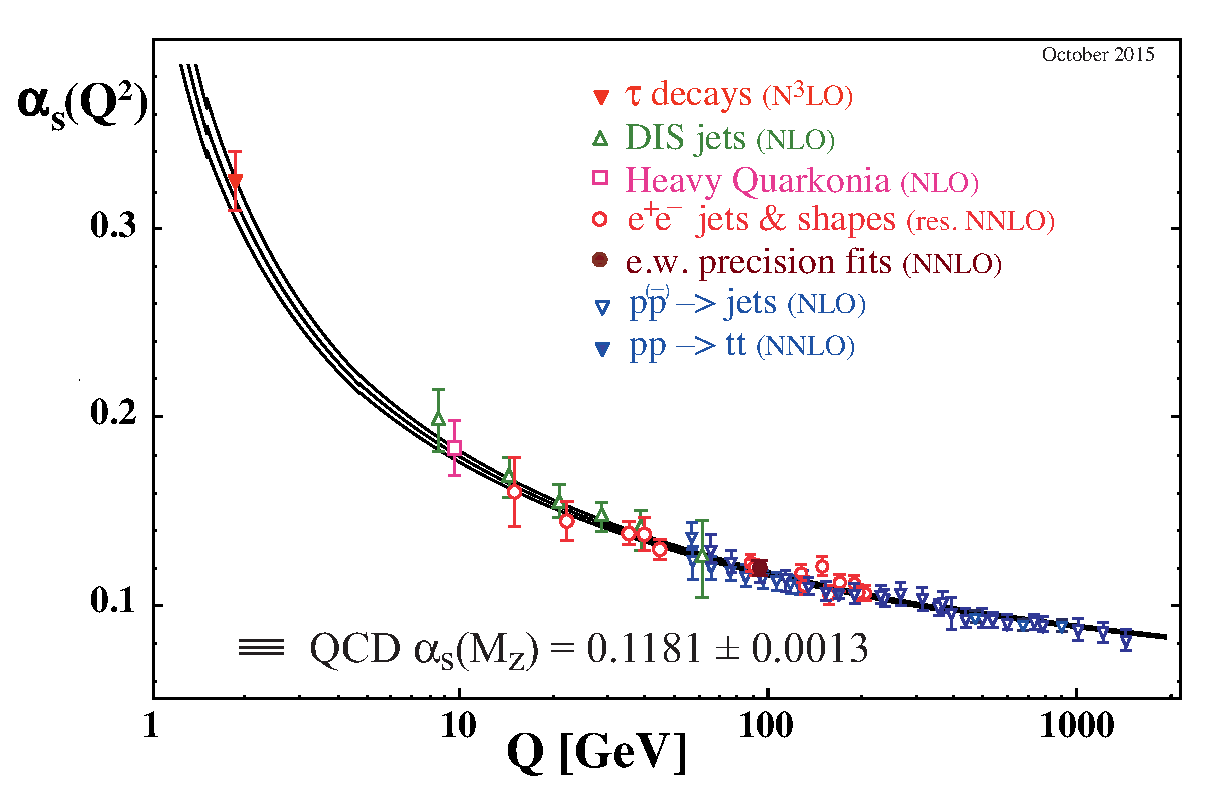
\includegraphics[width=0.6\textwidth]{figures/Theory/asq-2015.eps}
\captionsetup{width=0.85\textwidth} \caption{\small Evolution of the strong coupling constant $\alpha_s$ with energy scale $Q$, as probed by different measurements. From reference \cite{Bethke:2015etp}.}
\label{sec:theo:fig:alpha}
\efig


In the high-energy (i.e. short-distance) regime, $\alpha_{s}$ is sufficiently small that perturbation theory fully applies, and asymptotically quarks and gluons can be considered as free particles. This property is referred to as ``asymptotic freedom'' \cite{Politzer:1973fx,Gross:1973id}, and it is particularly important for the computability of cross sections at hadron colliders.
On the other hand, at lower energies (i.e. longer distances) $\alpha_{s}$ increases to the point of diverging; i.e. quarks and gluons cannot be found as free particles. This property is known as ``confinement'': when trying to separate two quarks, the potential energy increases enough that a quark-antiquark pair is created from the vacuum and colorless hadrons are eventually formed. Therefore, quarks and gluons produced as the result of interactions among particles at high energy will manifest themselves in the detector as collimated sprays of colorless hadrons called ``jets''.
At low energies ($Q<\Lambda_{\rm QCD}$), where the perturbative approximation is no longer valid, numerical (lattice QCD) or phenomenological (hadronisation models) approaches have to be used in order to describe this regime.

\subsection{Electroweak theory}

The gauge invariance of electromagnetism was already introduced in Maxwell's formulation of Electrodynamics \cite{maxwell1873treatise}. It was later extended to the invariance under a local phase transformation, which accommodated the explanation of the interaction in terms of Quantum ElectroDynamics (QED). The weak interaction was first identified by studying $\beta$-decays of atomic nuclei in the late 19th century. The experiments regarding these decays also lead to the postulation of neutrinos by Wolfgang Pauli \cite{Pauli:83286}, introduced to ensure the energy, momentum and spin conservation in these processes. After the parity violation of the weak processes was confirmed in the experiment conducted by C.-S. Wu \cite{Wu:1957my}, a new gauge theory formulation was constructed. The Wu experiment showed that the decay particles were travelling in a direction opposite to their spin, which suggested that the weak interaction had a form of a difference of a vector (representing the particle momentum) and an axial vector (representing the particle spin), i.e. a V-A form. The weak interaction is thus not the same for a particle and its mirror symmetric partner. This feature is referred to as the parity violation (P violation) of the weak interaction. It was shown later that the weak interaction violates as well the CP (charge conjugation and parity) symmetry \cite{Wolfenstein:1964ks} and the T (time reversal) \cite{Lees:2012uka}, but conserves CPT \cite{Lee:1965js}.\par
The electroweak theory describes the weak and the electromagnetic interactions, using a Lagrangian invariant under transformations of the symmetry group $SU(2)_{L} \otimes U(1)_{Y}$. The $SU(2)_{L}$ group introduces the weak isospin quantum number ($T$). The group is non-abelian and the commutation rules for the generators of the group are the following:
\be
\left [T_i , T_j \right ] = i \epsilon_{ijk} T_k,
\ee
\noindent where $\epsilon_{ijk}$ is the totally-antisymmetric Levi-Civita tensor and $T_i=\frac{\sigma_i}{2}$ $(i=1,2,3)$, where $\sigma_i$ are the Pauli matrices. Three bosons are introduced for $SU(2)_{L}$ according to the number of group generators. The fermions have different $SU(2)_{L}$ representation according to their chiral structure, defined as $f_{L,R}=\frac{1}{2}(1\mp \gamma_{5})f$, with $\gamma_{5}= i \gamma_{0}\gamma_{1}\gamma_{2}\gamma_{3}$. Left-handed fermions are weak-isospin doublets ($T_{3}=\pm1/2$) while right-handed fermions are singlets ($T_{3}=0$), where $T_{3}$ is the third component of the weak isospin. Only left-handed components participate in weak interaction, thus explaining the subscript in $SU(2)_{L}$. The abelian group $U(1)_{Y}$ introduces the hypercharge quantum number, $Y$, defined using the Gell-Mann-Nishijima formula:
\be
Q = T_{3}+\frac{Y}{2},
\ee

\noindent where $Q$ is the electric charge. \noindent Electric charge and hypercharge are quantities absolutely conserved.\\ Table \ref{chp:the:tab:particles} shows the multiplets of fermions fields and their $T$, $T_{3}$, $Y$ and $Q$ quantum numbers.

\begin{table}[t!]
\begin{center}
  \begin{tabular}{|c||c c c||c|c|c|c|}
  \hline
  & \multicolumn{3}{c}{Fermions multiplets}&$T$&$T_{3}$&$Y$&$Q$\\
     \hline \hline
    \multirow{2}{*}{Leptons}&$\begin{pmatrix} e\\ \nu_{e}\\ \end{pmatrix}_{L}$&$\begin{pmatrix} \mu\\ \nu_{\mu}\\ \end{pmatrix}_{L}$&$\begin{pmatrix} \tau\\ \nu_{\tau}\\ \end{pmatrix}_{L}$&$1/2$&$\begin{matrix}+1/2\\-1/2\\ \end{matrix}$&$-1$&$0$\\
    &$e_{R}$&$\mu_{R}$&$\tau_{R}$&0&0&$-2$&$-1$\\
\hline
 \multirow{3}{*}{Quarks}&$\begin{pmatrix} u\\ d^{\prime}\\ \end{pmatrix}_{L}$&$\begin{pmatrix} c \\ s^{\prime}\\ \end{pmatrix}_{L}$&$\begin{pmatrix} t \\ b^{\prime}\\ \end{pmatrix}_{L}$&$1/2$&$\begin{matrix}+1/2\\-1/2\\ \end{matrix}$&$+1/3$&$\begin{matrix}+2/3\\-1/3\\ \end{matrix}$\\
    &$u_{R}$&$c_{R}$&$t_{R}$&0&0&+4/3&+2/3\\
    &$d_{R}$&$s_{R}$&$b_{R}$&0&0&$-2/3$&$-1/3$\\
  \hline
\end{tabular}

\captionsetup{width=0.85\textwidth} \caption{\small Weak isospin multiplets. Here $d^{\prime}$, $s^{\prime}$, and $b^{\prime}$ denote flavour eigenstates, each of which can be expressed as a linear combination of the mass eigenstates ($d$, $s$, and $b$) weighted by CKM matrix elements \cite{cab,ckm}.}
\label{chp:the:tab:particles}
\end{center}
\end{table}


Under a local gauge transformation of the $SU(2)_{L} \otimes U(1)_{Y}$ group a fermionic field $\Psi(x)$ transforms as:
\be
\Psi(x) \to \Psi^{\prime}(x) = e^{\frac{i}{2}\vec{\sigma}\cdot \vec{\alpha}(x)}e^{i\frac{Y}{2}\beta(x)}\Psi(x).
\ee

\noindent To ensure local gauge invariance of the lagrangian the covariant derivative is introduced:
\be
D_{\mu}^{L}\equiv \partial_{\mu}+ig T_{i} W_{\mu}^{i}+ig^{\prime}\frac{Y}{2}B_{\mu}, \,\,\,\,\,\,\,\,
D_{\mu}^{R}\equiv \partial_{\mu}+ig^{\prime}\frac{Y}{2}B_{\mu} ,
\label{chp:theo:eq:EWderivative}
\ee
\noindent where $D_{\mu}^{L}$ acts on weak-isospin doublets and $D_{\mu}^{R}$, instead, on singlets. The coupling constants $g$ and $g^{\prime}$ are associated with the $SU(2)_{L}$ and $U(1)_{Y}$ gauge groups respectively, and $W_{\mu}^{i}$, $B_{\mu}$ denote the gauge fields of the respective gauge groups. The $SU(2)_{L}$ gauge fields transform as $\vec W_{\mu} \to \vec W_{\mu} -\frac{1}{g}\partial_{\mu} \vec \alpha - \vec \alpha\times \vec W_{\mu} $, while the $U(1)_{Y}$ gauge field transforms as  $B_{\mu}\to B_{\mu} -\frac{1}{g^{\prime}}\partial_{\mu}\beta$. \par
After introducing the covariant derivative and a kinetic term for the gauge fields, the EW Lagrangian is:
\be
\mathcal{L}_{\rm EW} = i \bar{f_{L}}\gamma^{\mu}D_{\mu}^{L}f_{L}+ i \bar{f_{R}}\gamma^{\mu}D_{\mu}^{R}f_{R} -\frac{1}{4} W_{\mu \nu}^{i} W^{\mu \nu}_{i} -\frac{1}{4} B_{\mu \nu} B^{\mu \nu},
\label{chp:the:eq:LEW}
\ee
\noindent where $i=1,2,3$, and $W_{\mu \nu}^{i}$ and $B_{\mu \nu}$ are the field tensors for $SU(2)_{L}$ and $U(1)_{Y}$ respectively, defined as:
\be
W_{\mu \nu}^{i}=  \partial_{\mu} W_{\nu}^{i}-\partial_{\nu} W_{\mu}^{i}-g\epsilon_{ijk} W_{\mu}^{j}W_{\nu}^{k}, \,\,\,\,\,\,\,\,
B_{\mu \nu}=  \partial_{\mu} B_{\nu}-\partial_{\nu} B_{\mu}.
\ee
The introduction of mass terms for gauge fields ($\frac{1}{2}M_{V}^{2}W_{\mu}W^{\mu}$) or fermion fields ($-mf_{L}f_{R}$) in equation \ref{chp:the:eq:LEW} would violate the local gauge invariance under $SU(2)_{L} \otimes U(1)_{Y}$, since those terms couple left- and right-handed components. 
Breaking gauge invariance would consequently break the renormalisability of the SM. Therefore, a mechanism for generating non-zero masses while preserving the renormalisability of the theory needs to be introduced to be consistent with the experimental observation of massive fermions and vector bosons.

\subsection{The Brout-Higgs-Englert mechanism}

The Brout-Higgs-Englert (BEH) mechanism \cite{HiggsOriginal2,HiggsOriginal,Higgs:1964ia,Guralnik:1964eu} solves the apparent contradiction between massive particles and the requirement of gauge invariance. This mechanism triggers a Spontaneous Symmetry Breaking (SSB), $SU(2)_{L} \otimes U(1)_{Y} \to U(1)_{\rm EM}$, where $U(1)_{\rm EM}$ denotes the gauge group describing electromagnetism. The SSB is triggered by introducing a complex scalar field. This field, referred to as ``Higgs field'', must have the form of a $SU(2)_{L} \otimes U(1)_{Y}$ multiplet in order to satisfy the SM gauge invariance. In the so called ``minimal'' Higgs sector, the Higgs field is an $SU(2)_{L} \otimes U(1)_{Y}$-isodoublet with isospin $T =1/2$ and the hypercharge $Y= 1$:

\be
\Phi=\begin{pmatrix} \phi^{+}\\ \phi^{0}\\ \end{pmatrix},
\ee

\noindent containing one positively-charged component $\phi^{+}$ and one neutral component $\phi^{0}$. \par
The dynamics of this field, which will be added to the $\mathcal{L}_{\rm EW}$, is given by the Lagrangian:

\be
\mathcal{L}_{\rm Higgs}=(D_{\mu}\Phi)^{\dagger}D^{\mu}\Phi -V(\Phi),
\ee

\noindent where $D_{\mu}$ is the covariant derivative (see equation \ref{chp:theo:eq:EWderivative}) and the potential $V(\Phi)$ is:

\be
 V(\Phi)=\mu^{2}\Phi^{\dagger}\Phi+\lambda(\Phi^{\dagger}\Phi)^{2}.
 \ee

In order for $V(\Phi)$ to have at least one stable minimum $\lambda$ is required to be positive. For $\lambda>0$, two possibilities arise: $\mu^{2}>0$ and $\mu^{2}<0$, which are illustrated in figure \ref{fig:theo:higgspotential}. 
\begin{figure}[h!]
\begin{subfigure}{0.5\textwidth}
  \centering
  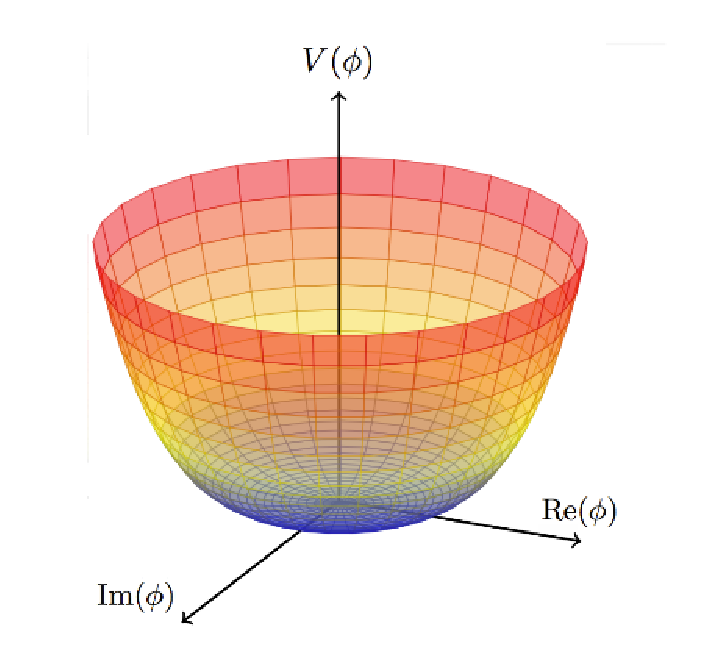
\includegraphics[width=0.9\textwidth]{figures/Theory/higgs1.eps}
  \caption{}
  \label{fig:theo:higgs1}
\end{subfigure}
\begin{subfigure}{0.5\textwidth}
  \centering
  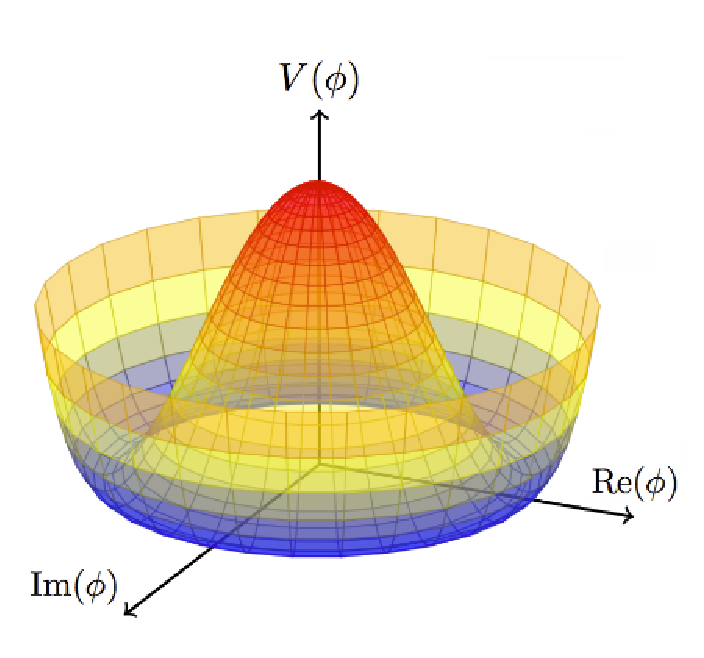
\includegraphics[width=0.9\textwidth]{figures/Theory/higgs2.eps}
  \caption{}
  \label{fig:theo:higgs2}
\end{subfigure}

\captionsetup{width=0.85\textwidth} \caption{\small Vacuum potential for $\lambda>0$ and (a) $\mu^{2}>0$ or (b) $\mu^{2}<0$, with the typical shape of a Mexican hat.}
\label{fig:theo:higgspotential}
\end{figure}
In the first case, $\mu^{2}>0$, there is a single solution to the minimisation which corresponds to $|\Phi|= 0$ and provides a vacuum expectation value (VEV), $\langle \Phi \rangle_{0}=\langle 0|\Phi|0 \rangle= 0$. If $\mu^{2}<0$, there is no unique minimum with a VEV, $\langle \Phi \rangle_{0}=\langle 0|\Phi|0 \rangle= v/\sqrt{2}$ and the potential $V(\Phi)$ presents a ``Mexican hat'' shape (figure \ref{fig:theo:higgs2}) with its minimum at:
\be
\Phi^{\dagger}\Phi=-\frac{\mu^{2}}{2\lambda}=\frac{v^{2}}{2},
\ee

\noindent where $v=\sqrt{-\mu^{2}/\lambda}$. In this case, the fundamental vacuum state is no longer invariant
under $SU(2)_{L} \otimes U(1)_{Y}$, meaning that these two symmetries are now broken. When a continuous symmetry is broken Goldstone bosons,  massless scalars, are present (Goldstone theorem \cite{PhysRev.127.965}) and they can be absorbed by a gauge field as a longitudinal polarisation component, resulting in the gauge field acquiring mass. Since the photon is the only electroweak boson known to be massless, the minimum of the potential is chosen so that the Higgs field that acquires a VEV is the one with zero electric charge in order to not break $U(1)_{\rm EM}$:

\be
\Phi_{0}=\frac{1}{\sqrt{2}}\begin{pmatrix} 0\\ v\\ \end{pmatrix}.
\ee

\noindent An infinitesimal $SU(2)_{L}$ transformation around the vacuum can then be expressed as:

\be
\Phi^{\prime}(x)=\frac{e^{i\vec \sigma\cdot \vec \theta(x)/v}}{\sqrt{2}}\begin{pmatrix} 0\\ v + H(x)\\ \end{pmatrix},
\ee

\noindent with $H(x)$ denoting a real scalar field associated to a physical degree of freedom, the Higgs-boson particle, and $\theta$ denoting the three fields which will be absorbed by the gauge fields.
With this choice of the vacuum and the gauge, the Lagrangian of the physical Higgs field reads:

\be
\mathcal{L}_{\rm Higgs}=(D_{\mu}H)^{\dagger}D^{\mu}H -\frac{1}{2}(-2\mu^{2})H^{2}-\lambda v H^{3}-\frac{1}{4}\lambda H^{4},
\ee

\noindent where the second term corresponds to the tree-level mass term of the $H(x)$ field, $m_{H}=\sqrt{-2\mu^{2}}=\sqrt{2\lambda}v$, and the last two terms describe interactions among Higgs fields. Since the value of $\lambda$  is unknown, $m_{H}$ is not predicted by the theory and must be determined experimentally.\par
Furthermore, this procedure has also generated the masses of the gauge bosons. This becomes obvious from the development of $|D_{\mu}\Phi^{\prime}|^{2}$, which provides terms of the form:

\begin{equation}
  \begin{split}
    & \left|\left(-ig\frac{\vec \sigma}{2}\vec{W}_\mu - i\frac{g'}{2}B_\mu \right)\Phi\right|^2 
    = \frac{1}{8} \left|\left(
    \begin{matrix}
      gW_\mu^3 + g'B_\mu & g(W_\mu^1 - iW_\mu^2) \\
      g(W_\mu^1 + iW_\mu^2) & -gW_\mu^3 + g'B_\mu 
    \end{matrix}
    \right)
    \left(
    \begin{matrix}
      0 \\%
      v   \
    \end{matrix}
    \right) \right|^2 \\
    &= \frac{1}{8} v^2 g^2 \left[(W_\mu^1)^2 + (W_\mu^2)^2\right] + \frac{1}{8} v^2 (g'B_\mu - gW_\mu^3)(g'B^\mu - gW^{3\mu}) \\
    &= \left(\frac{1}{2}vg\right)^2 W_\mu^{+} W^{-\mu} + \frac{1}{8} v^2 \left(W_\mu^3, B_\mu\right) 
    \left(
    \begin{matrix}
      g^2 & -gg' \\
      -gg' & g'^2
    \end{matrix}
    \right)
    \left(
    \begin{matrix}
      W_\mu^3 \\
      B_\mu
    \end{matrix}
    \right),
  \end{split}
  \label{eq:HiggsBosonMassDemonstration}
\end{equation}

\noindent defining the charged fields as $W^{\pm} = (W^1 \mp iW^2)/\sqrt{2}$. The mass eigenstates can be obtained diagonalizing the mass matrix, and expressed as a function of $W_\mu^3$ and $B_\mu$:

\begin{equation}
\begin{split}
    \frac{1}{8}v^2\left[g^2\left(W_\mu^3\right)^2 - 2gg'W_\mu^3 B^\mu + g'^2B_\mu^2\right] 
    =\ & \frac{1}{8}v^2\left[ gW_\mu^3 - g'B_\mu\right]^2           \\
    &+ 0 \left[g'W_\mu^3 + gB_\mu\right]^2 \\
    =\ & \frac{1}{2}\left(v\frac{\sqrt{g^2+g'^2}}2\right)^2 Z_\mu^2 \\
    &+ 0 \cdot A_\mu^2, 
\end{split}
  \label{eq:HiggsBosonMassDemonstration2}
\end{equation}

\noindent where $Z_\mu$ and $A_\mu$  can be defined as:

\begin{equation}
  Z_\mu = \frac{gW_\mu^3 - g'B_\mu}{\sqrt{g^2 + g'^2}}= \cos \theta_{W} W^{3}_{\mu}-\sin \theta_{W} B_\mu,
  \label{eq:HiggsZdefinition}
\end{equation}
\begin{equation}
  A_\mu = \frac{g'W_\mu^3 + gB_\mu}{\sqrt{g^2 + g'^2}}=\sin \theta_{W} W^{3}_{\mu}+\cos \theta_{W} B_\mu,
  \label{eq:HiggsAdefinition}
\end{equation}
\noindent representing the fields associated with the $Z$ boson and the photon respectively, and $\theta_{W}$ is the Weinberg angle, $\tan \theta_W = g^{\prime}/g$.
From equations \ref{eq:HiggsBosonMassDemonstration} and \ref{eq:HiggsBosonMassDemonstration2}, the tree level predictions for masses of the gauge bosons and the relation between the coupling constants can be derived:

\be
 m_W = \frac{vg}{2}=m_Z \cos \theta_{W}, 
\ee

\be
m_Z = v \frac{\sqrt{g^2 + g'^2}}{2},
\ee
\be
 m_\gamma = 0.
 \ee


The BEH mechanism can provide as well mass to the fermions, by postulating their coupling to the Higgs boson via a Yukawa interaction:

\be
\mathcal{L}_{\rm Yukawa}=\displaystyle\sum_{f=\ell,q}y_{f}\left[ \bar{f}_{L}\Phi f_{R}+\bar{f}_{R}\bar{\Phi} f_{L}\right],
\label{chp:theo:eq:yukawa}
\ee

\noindent where the matrices $y_{f}$ describe the Yukawa couplings between the Higgs doublet and the fermions. The Yukawa Lagrangian is gauge invariant since the combinations $\bar{f}_{L}\Phi f_{R}$ and $\bar{f}_{R}\bar{\Phi} f_{L}$ are $SU(2)_{L}$ singlets. The $y_{f}$ matrices can be diagonalised to obtain the eigenvalues of the Yukawa couplings using unitary transformations that will redefine the fermion fields. In the leptonic sector this transformation has no effect given the absence of right-handed neutrinos, while in the quark sector, the rotation to the mass eigenstate basis introduces a mixing among fermion families that is manifest in the weak interactions. The mixing between the weak eigenstates of the down-type quarks,\footnote{By convention, the mixing takes place between down-type quarks only, while the up-type mass matrix is diagonal.} $d^{\prime}$, $s^{\prime}$ and $b^{\prime}$, and the corresponding mass eigenstates $d$, $s$ and $b$, is described by the Cabibbo-Kobayashi-Maskawa (CKM) matrix \cite{ckm}. Off-diagonal elements of the CKM matrix have the result that $W$ bosons can couple to two quark belonging to two different families. The CKM matrix is fully specified by four parameters: three mixing angles controlling the mixing between each family pair and one complex phase responsible for CP-violating phenomena.\par
The tree-level predictions for the mass of the fermions are obtained introducing the expansion of the Higgs doublet in equation \ref{chp:theo:eq:yukawa}:

\be
m_{f}=\frac{y_{f}v}{\sqrt{2}}.
\ee

\noindent While the gauge-boson masses can be determined from the known values of the coupling constants $g$ and $g^{\prime}$, the fermion masses are free parameters, since their Yukawa couplings $y_{f}$ are not predicted by the SM. 


\subsection{Higgs boson production and decay in the Standard Model}

The most important production modes for the SM Higgs boson at the LHC are displayed in figure \ref{fig:theo:higgsprod}, with their cross sections shown in figure \ref{fig:theo:higgsxsec}.
The dominant production mechanism is gluon-gluon fusion (ggF) mediated by a virtual quark loop, where the main contribution is from the top quark, owing to its large Yukawa coupling.
The ggF production mode gives access to the top-quark Yukawa coupling under the assumption that no new particles are contributing to the loop. The vector-boson fusion (VBF) mode, whose cross section is about one order of magnitude smaller than for ggF, is an important Higgs-boson production mechanism due to the two forward jets that can be exploited to suppress backgrounds.
The associated production with a vector boson (VH) which, like VBF, allows to measure the Higgs boson couplings to weak gauge bosons, is suppressed compared to ggF and VBF since it needs an antiquark in the initial state.\footnote{VH was the second leading production mode at the Tevatron, after ggF.} The $b\bar{b}H$ and $t\bar{t}H$ production modes have the lowest cross sections but they can provide direct access to the third-generation quark Yukawa couplings in production mode.\par
The branching ratios for the different SM Higgs boson decay modes \cite{lhcxs} as function of its mass are shown in figure \ref{fig:theo:higgsbr}. For a mass of about 125 $\gev$ the $H \to b\bar{b}$ decay mode is dominant. The channels with the cleanest experimental signature are $H \to \gamma\gamma$ and $H\to ZZ^* \to 4\ell$ and, despite their small branching ratio, played a crucial role in the Higgs boson discovery.  

\begin{figure}[htb!]
  \centering
  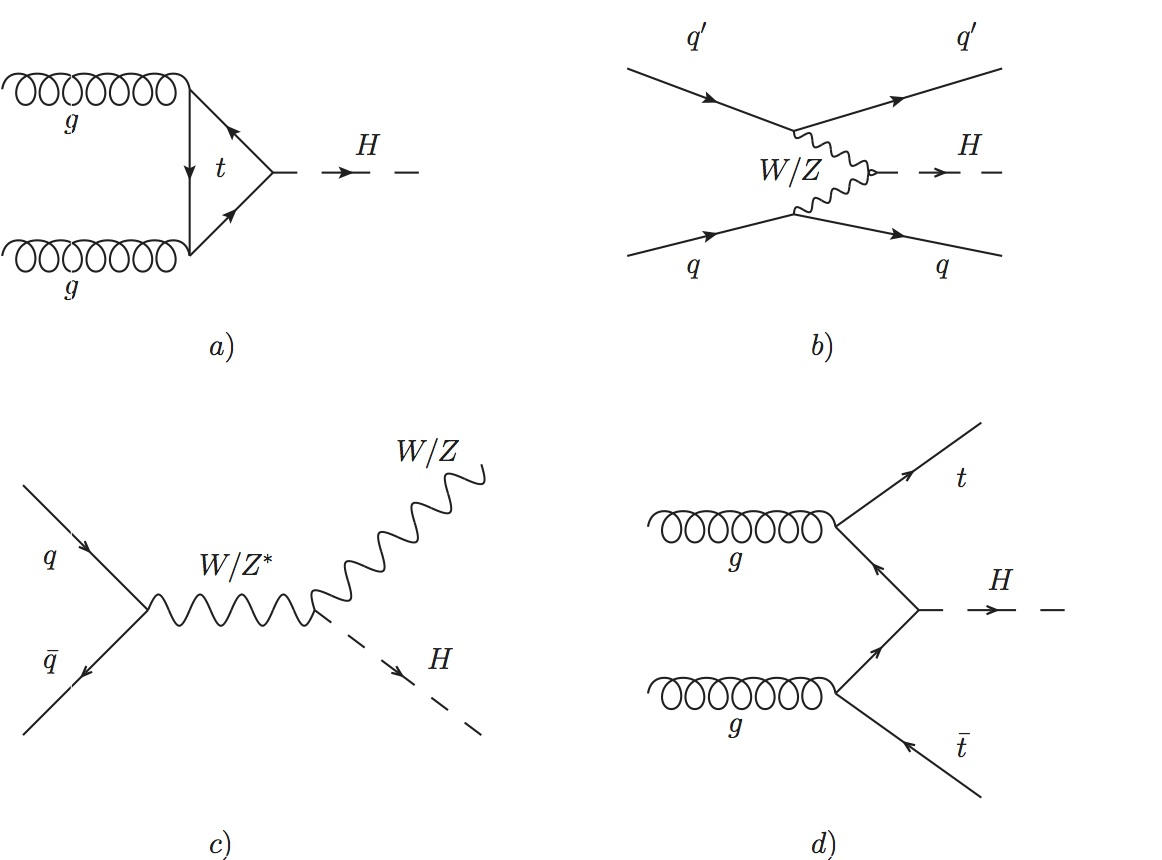
\includegraphics[width=0.7\textwidth]{figures/Theory/h-prod.png}
\captionsetup{width=0.85\textwidth} \caption{\small Representative Feynman diagrams for the most important production modes for the SM Higgs boson at the LHC (a) gluon-gluon fusion (b) vector-boson fusion (c) associated production with a vector boson and (d) $t\bar{t}H$ production. }
\label{fig:theo:higgsprod}
\end{figure}


\begin{figure}[htb!]
\begin{subfigure}{0.5\textwidth}
  \centering
  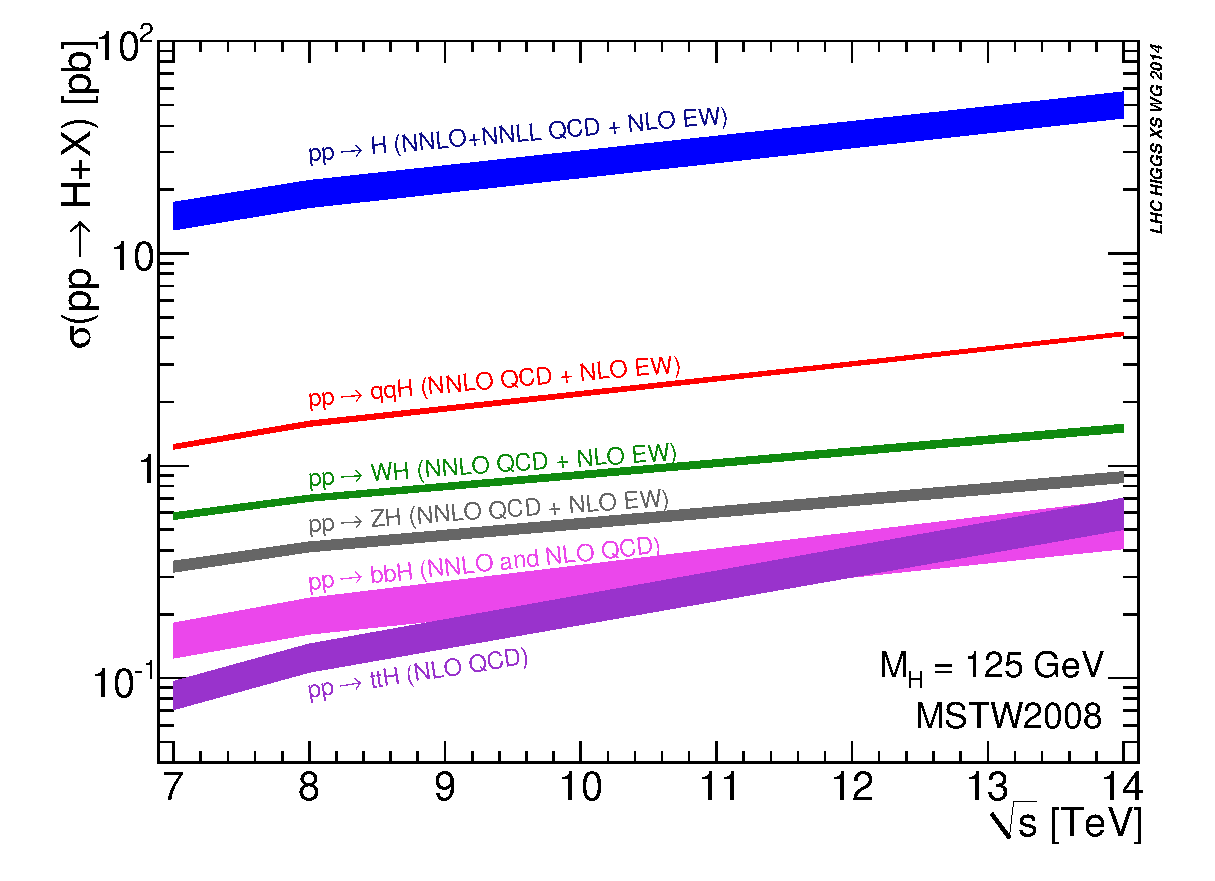
\includegraphics[width=0.9\textwidth]{figures/Theory/higgsxsec.eps}
  \caption{}
  \label{fig:theo:higgsxsec}
\end{subfigure}
\begin{subfigure}{0.5\textwidth}
  \centering
  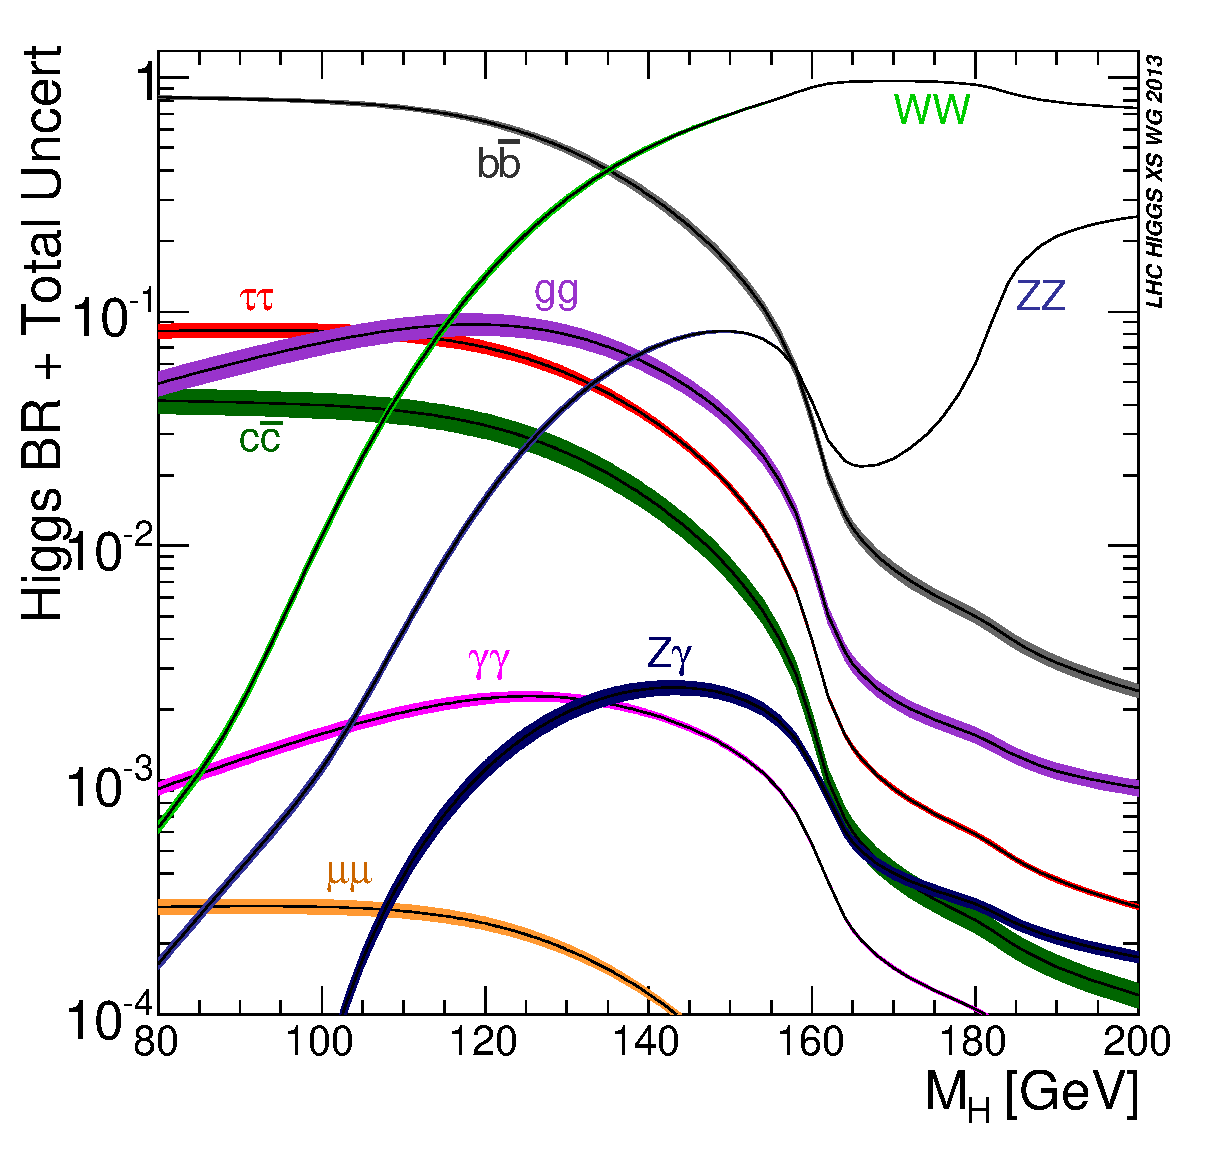
\includegraphics[width=0.7\textwidth]{figures/Theory/HiggsBR.eps}
  \caption{}
  \label{fig:theo:higgsbr}
\end{subfigure}

\captionsetup{width=0.85\textwidth} \caption{\small (a) Higgs-boson production cross sections  as a function of centre-of-mass energy and (b) branching ratios as a function of the Higgs-boson mass. The SM-like Higgs boson is assumed to have a mass of $m_{H}$=125 $\gev$. From reference \cite{lhcxs}.}
\label{fig:theo:higgsxsecbr}
\end{figure}


\subsection{Experimental tests and limitations of the Standard Model}

The SM has so far shown a remarkable success. It is a mathematically-consistent theory accommodating most experimental findings, with an excellent predictive power due to its renormalisability. During the 1970s and 1980s many discoveries set the scene for the success of the SM: the discovery of neutral current processes \cite{Hasert:1973ff}, the discovery of the charm \cite{PhysRevLett.33.1406,PhysRevLett.33.1404} and bottom \cite{Herb:1977ek} quarks, the $\tau$ lepton and its neutrino \cite{Perl:1975bf,Kodama:2000mp}, the discovery of the gauge bosons of the weak interaction $W$ and $Z$ \cite{Arnison:1983rp,Banner:1983jy,Arnison:1983mk,Bagnaia:1983zx}. In the 1990s the precision era of the electroweak sector started at CERN's Large Electron Positron (LEP) Collider. Many precision measurements of SM quantities were performed and, together with accurate theoretical calculations of radiative corrections, allowed to check the consistency of the model at permille level, which in turn allowed to derive indirect constraints on unknown parameters. In this context, the top-quark mass was precisely predicted from radiative corrections to the $W$-boson mass and the $Z\to b\bar{b}$ branching ratio, prior to the discovery of the top quark in 1995 by the CDF and D0 Collaborations \cite{topdisc_cdf,topdisc_d0} at Fermilab's Tevatron Collider. The discovery of the Higgs boson in July 2012 by the ATLAS and CMS Collaborations \cite{Aad:2012tfa,Chatrchyan:2012ufa} allowed to measure the last free parameter of the SM, the Higgs-boson mass of about 125 $\gev$ \cite{Aad:2015zhl}. Further measurements of the spin and CP of this particle confirmed that it is a scalar with positive CP eigenstate \cite{Aad:2013xqa,Khachatryan:2014kca}. As of today, the couplings to the SM particles \cite{Khachatryan:2016vau} have been found to be in agreement with those of the SM Higgs boson.\par
The validity of the SM can be tested performing a global electroweak fit using as input many precision measurements. The fit results, performed by the GFitter Collaboration \cite{Baak:2013ppa}, are shown in figure \ref{fig:theo:fit1}.
\begin{figure}[t!]
\begin{subfigure}{0.5\textwidth}
  \centering
  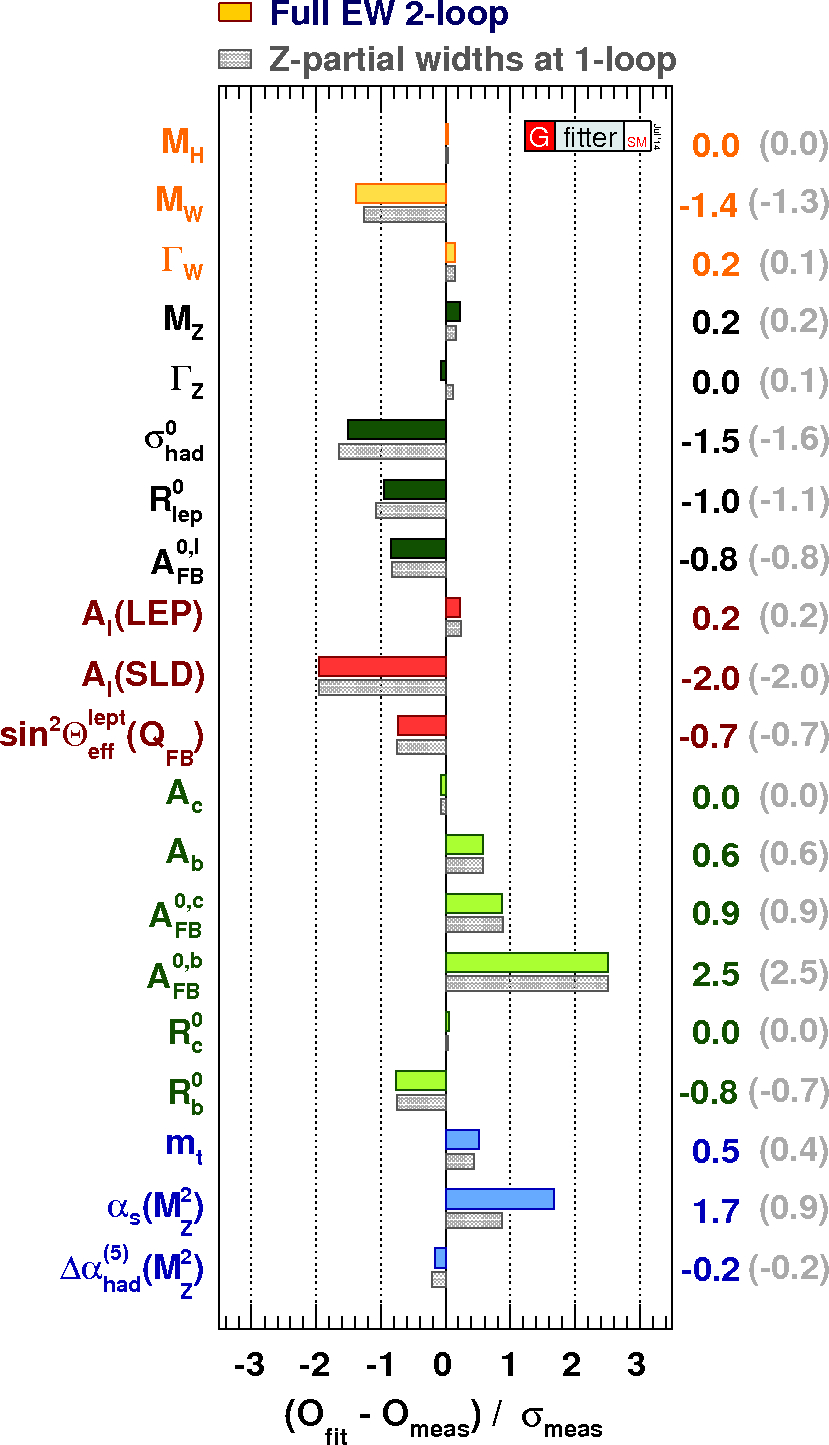
\includegraphics[width=0.5\textwidth]{figures/Theory/fit1.jpg}
  \caption{}
  \label{fig:theo:fit1}
\end{subfigure}
\begin{subfigure}{0.5\textwidth}
  \centering
  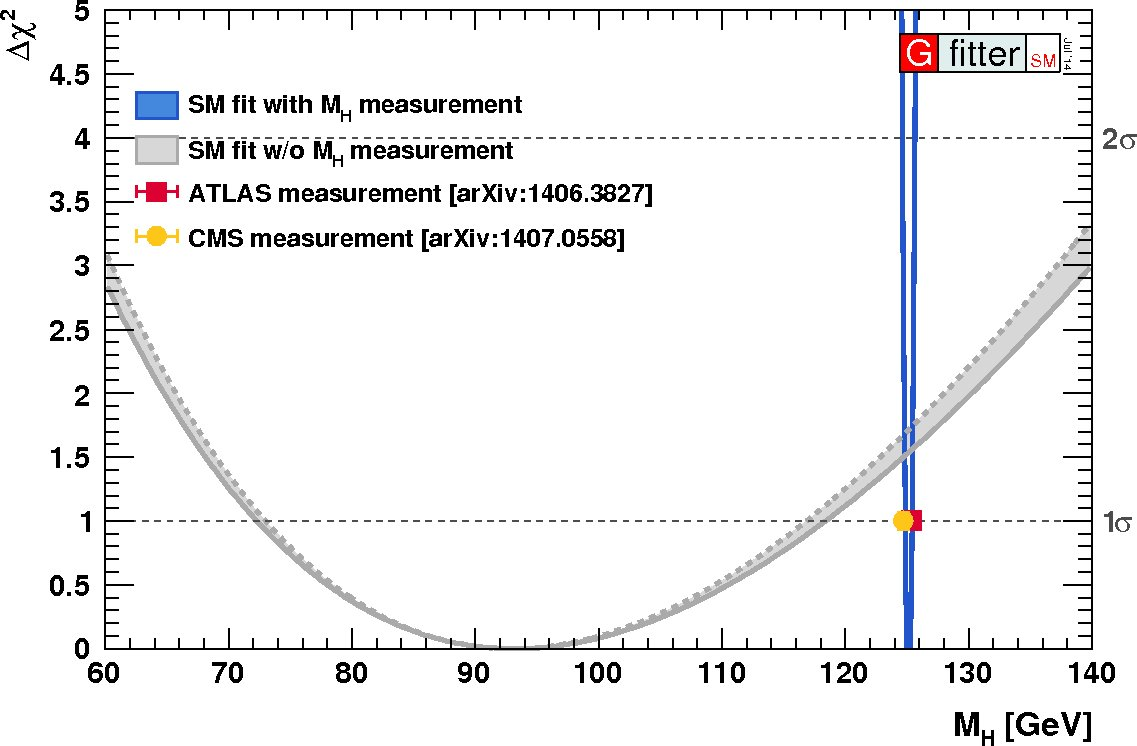
\includegraphics[width=0.9\textwidth]{figures/Theory/fit2.jpg}
  \caption{}
  \label{fig:theo:fit2}
\end{subfigure}

\captionsetup{width=0.85\textwidth} \caption{\small (a) Pull values for the SM fit, i.e. deviations between experimental measurements and theoretical calculations in units of the experimental uncertainty. (b) $\chi^{2}$ as a function of Higgs-boson mass $M_{H}$, with (blue band) and without the $M_{H}$ measurements (gray band). From reference \cite{Baak:2013ppa}.}
\label{fig:theo:ewfit}
\end{figure}
Good consistency between measured and expected quantities is found and none of the observed differences exceeds three standard deviations. From this fit, leaving the mass of the Higgs boson as free parameter, it was predicted to be $94.1^{+25}_{-22}$ $\gev$, within 1.5 standard deviations from the current measurement (see figure \ref{fig:theo:fit2}). 

Despite its tremendous success, a number of theoretical and experimental arguments suggest that the SM is not the ultimate theory of Nature, but more likely just a low-energy manifestation, i.e. an effective theory, of a more general theory.
Gravity is not accommodated in this model, since no renormalisable quantum gravity theory is available. The SM is not a complete unified theory, but rather describes three of the four forces present in Nature using a convolution of different symmetries and not as a single symmetry group. Grand Unified Theories (GUTs) try to unify these three symmetry groups in a single symmetry group $G$, $G\supset SU(3)_{C} \otimes SU(2)_{L} \otimes U(1)_{Y}$, while Theories of Everything try to add gravity as well.
An additional indication of the SM not being complete unified theory, besides the ones already discussed, is that the forces are expected to unify at high energy since their couplings depend on the energy scale but, as shown in figure \ref{sec:theo:fig:unification}, there is no convergence of the three couplings to a common value.

\bfig[t!]
\centering
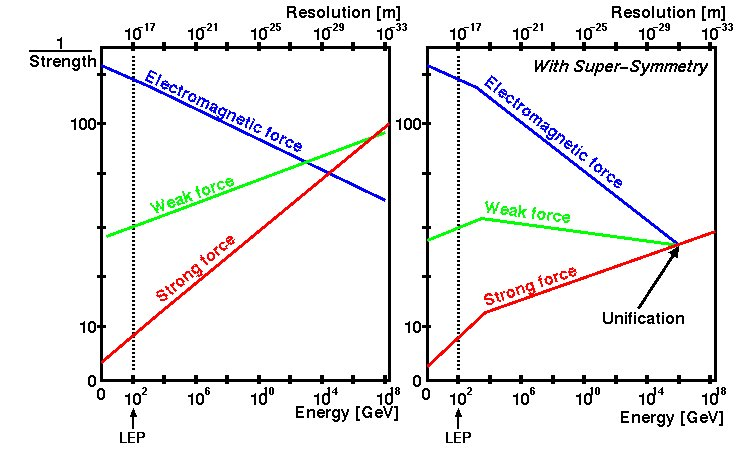
\includegraphics[width=0.7\textwidth]{figures/Theory/unification.jpg}
\captionsetup{width=0.85\textwidth} \caption{\small Running of couplings (a) in the SM and (b) in a hypothetical Supersymmetric Model as function of the energy scale.}
\label{sec:theo:fig:unification}
\efig


The SM provides no explanation for the baryon (i.e. matter-antimatter) asymmetry in the universe \cite{Sakharov:1967dj}, which is connected to CP violation, since the amount of CP violation predicted by the SM is not enough to explain such asymmetry. The energy density of the universe made by ordinary baryonic matter according to several astronomical observations, from rotation curves of galaxies \cite{Begeman:1991iy} to gravitational lensing \cite{Ade:2013zuv}, is only for a $\sim5\%$, the remaining component being dark matter ($\sim25\%$) and dark energy ($\sim70\%$). The SM does not provide a particle candidate to explain the large amount of dark matter in the universe. Also, it does not explain dark energy. The observation of neutrino oscillations and hence the fact that neutrinos are massive \cite{Fukuda:1998mi} cannot be explained in the SM. Extending the SM Lagrangian to accomodate massive neutrinos can be achieved by introducing right-handed neutrinos or by describing them as Majorana particles.
The SM has already 19 arbitrary parameters, out of them nine fermion masses, and it would have even more if neutrinos masses were added.
There is no explanation for why there are exactly three generations of chiral fermions and why their masses are so different, i.e. which mechanism generates their Yukawa couplings. The arbitrariety of parameters in the SM, and in particular of the fermion masses, introduces the naturalness problem \cite{Giudice:2008bi}. A ``natural'' theory is characterised by free parameters with values of the same order of magnitude. This does not happen in the SM, where some masses differ by several orders of magnitude. If the SM is assumed as the ``final theory'' valid up to the Planck scale, it exhibits an additional problem known as the ``hierarchy problem'' coming from the huge difference between the electroweak and the Planck scales ($M_{\rm Pl}/m_{W}\sim10^{17}$) and its effect on the Higgs boson mass. Unlike fermion and gauge boson masses, which are protected by chiral or gauge symmetries, the mass of an elementary scalar receives radiative corrections from vacuum polarisation diagrams (see figure \ref{fig:theo:higgsmasscorr}) of the order of the largest energy scale involved in the theory:

\be
m_{H}^{2}=(m_{H})_{0}^{2}+\delta m_{H}^{2}=(m_{H})_{0}^{2}-\frac{|y_{f}|^{2}}{16\pi^{2}}\left[ 2\Lambda^{2} +\mathcal{O}\left( m_{f}^{2}\ln\left(\frac{\Lambda}{m_{f}}\right) \right) \right],
\label{sec:theo:eq:higgcorr}
\ee  

\noindent where $(m_H)_0$ is the bare Higgs-boson mass, $y_{f}$ and $m_{f}$ are the Yukawa coupling and the mass, respectively, of the fermion $f$ involved in the loop, and $\Lambda$ is the energy scale up to which the SM is still valid. The top quark is responsible for the largest correction due to its large Yukawa coupling, $y_{t}\sim1$; thus the top quark might have a special role in the electroweak symmetry breaking mechanism and the mass hierarchy pattern. If $\Lambda$ is set to $M_{\rm Pl}$, the quantum corrections to the Higgs boson mass can be up to 30 orders of magnitude larger than the measured Higgs boson mass squared. To recover the measured mass, the value of the bare Higgs-boson mass and the corrections have to cancel with an incredible precision, referred to as ``fine tuning''. Although this lucky cancellation could in principle happen in Nature, it is considered highly ``unnatural'' and several extensions of the SM have been proposed to stabilise the Higgs boson mass.


\begin{figure}[htb!]
\begin{subfigure}{0.5\textwidth}
  \centering
  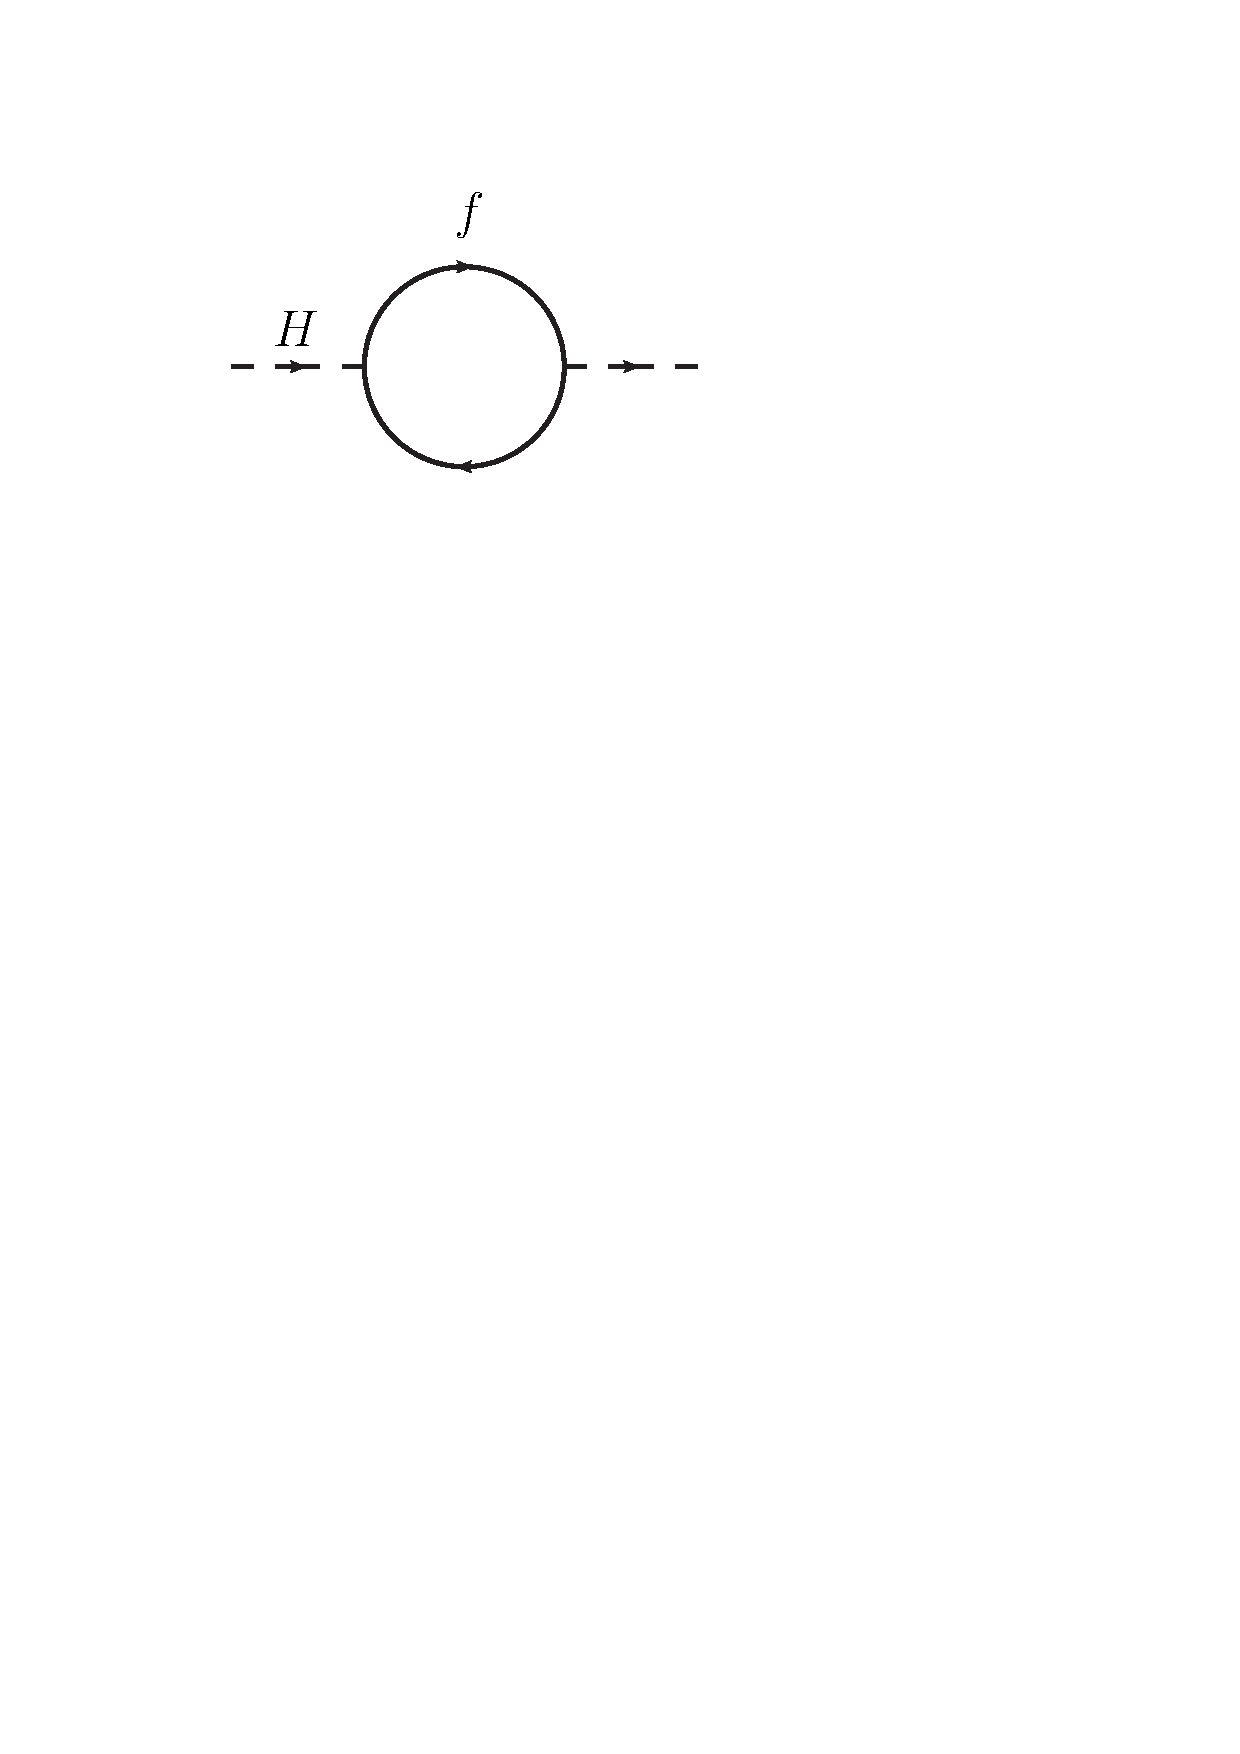
\includegraphics[width=0.5\textwidth]{figures/Theory/loopFermion.pdf}
  \caption{}
  \label{fig:theo:higgscorrectionloopfermion}
\end{subfigure}
\begin{subfigure}{0.5\textwidth}
  \centering
  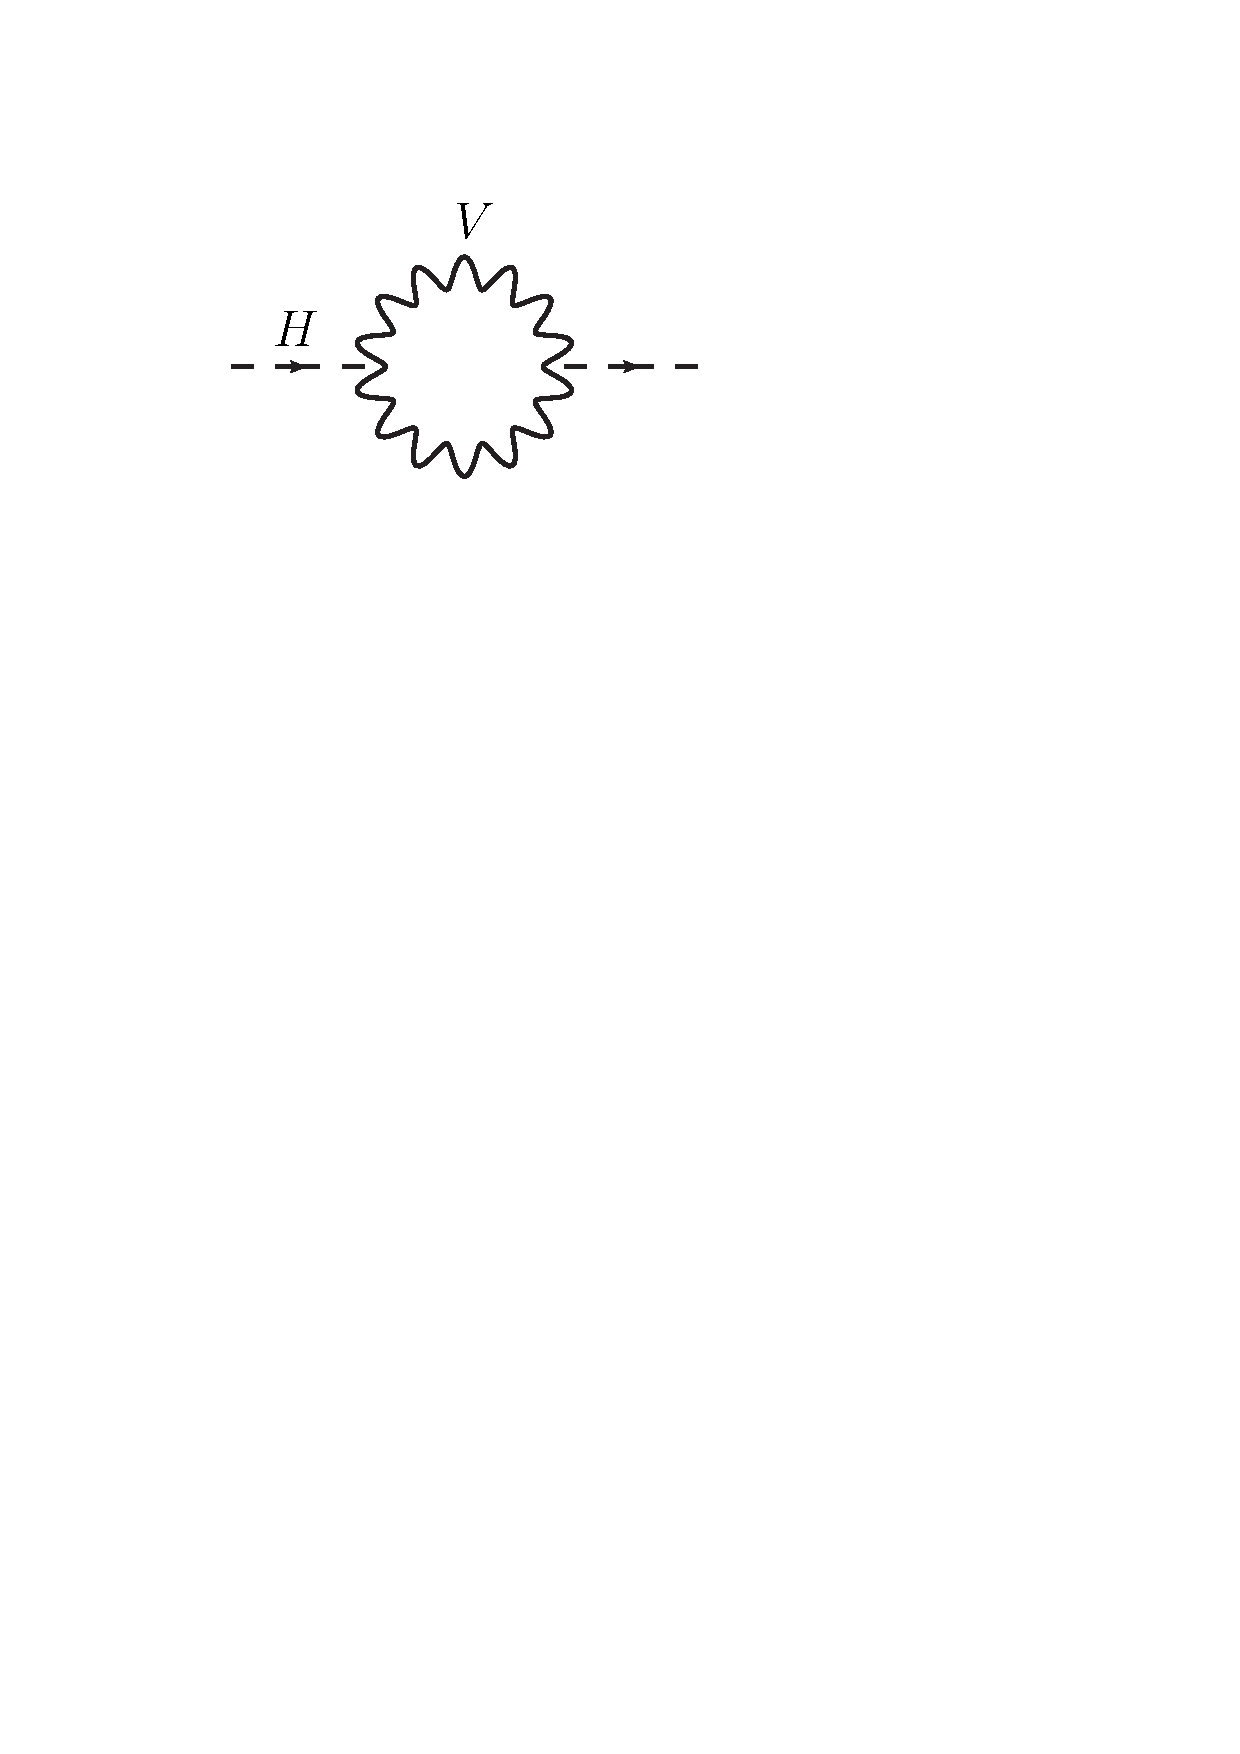
\includegraphics[width=0.5\textwidth]{figures/Theory/loopBoson.pdf}
  \caption{}
  \label{fig:theo:higgscorrectionloopboson}
\end{subfigure}

\captionsetup{width=0.85\textwidth} \caption{\small Examples of one-loop quantum corrections to the Higgs-boson mass due to (a) fermions and (b) vector bosons.}
\label{fig:theo:higgsmasscorr}
\end{figure}

\section{Beyond the Standard Model}
Over the years, many theories have been developed to solve one or more of the SM shortcomings, but so far none of these theories have found experimental support yet. In the following sections, some of these scenarios for physics beyond the SM are reviewed, with a focus on those predicting new phenomena of interest for this dissertation.

\subsection{Supersymmetry} 
Supersymmetric models introduce a new symmetry, referred to as ``supersymmetry'' (SUSY), which transforms a bosonic state into a fermionic state and viceversa, being the last possible extension of the Lorentz group \cite{Haag:1974qh,Drees:1996ca}. This symmetry introduces a superpartner for each SM particle. The existence of those partners can stabilise the Higgs-boson mass, solving the hierarchy problem. In fact, if a new boson $S$, which couples to the Higgs boson, is introduced for each fermion $f$ the correction to the Higgs-boson mass due to this boson will be:

\be
\delta m_{H}^{2}=\frac{y^{2}_{S}}{16\pi^{2}}\left[2\Lambda^{2}+\mathcal{O}\left( m_{S}^{2}\ln\left( \frac{\Lambda}{m_{S}}\right) \right) \right].
\ee  

\noindent Bose-Einstein statistics implies an opposite sign with respect to the fermion mass correction shown in equation \ref{sec:theo:eq:higgcorr}. Therefore, if $y_{S} = |y_{f}|$, each of the fermion terms have a counter term that naturally cancels the quadratic divergence introduced. The residual correction left, ignoring the logarithmic contribution, is proportional to the quadratic mass difference between the fermion and the boson:

\be
\delta m_{H}^{2}=\frac{y^{2}_{f}}{16\pi^{2}}|m_{S}^{2}-m_{f}^{2}|.
\ee

\noindent According to the the ``naturalness'' argument, these corrections must not be much greater than $m_{H}$ in order to avoid too much fine tuning. This argument, not strict but quite desirable, sets the scale of the SM validity around the $\tev$, where the supersymmetric theory would replace the SM up to the Plank scale. Supersymmetry naturally predicts superpartners with the  same mass as the SM particles but, since no supersymmetric particles have been observed yet, supersymmetry must be a broken symmetry at low energy \cite{Martin:1997ns,Witten:1981nf} and so the masses of the superpartners have to be beyond the reach of current experiments.\par
Supersymmetry is not a fixed model but rather a framework that allows many SM extensions depending on the number of generators in the symmetry group, as well as the composition and arrangement of the SM particles into supermultiplets. The Minimal Supersymmetric SM (MSSM) is a model that introduces the minimal number of new particles. It obeys to the same gauge symmetry of the SM, but it doubles the spectrum of particles, since for every partner of the SM, a superpartner is postulated, differing by half a unit of spin. Spin-0 superpartners of the fermions are denoted starting with an extra ``s'' (e.g. the selectron is the superpartner of the electron) while the spin-1/2 superpartners of the bosons are added the suffix ``ino'' (e.g. the gluino is the superpartner of the gluon). Table \ref{sec:theo:tab:MSSM_content} summarises the MSSM particle content. 

\begin{table}[!ht]
  \begin{center}
    \begin{small}
      %\setlength{\tabcolsep}{0.0pc}
      %\begin{tabular*}{\textwidth}{@{\extracolsep{\fill}}ccccc}
      \begin{tabular}{ccccc}
        \toprule
        \toprule
        \textbf{Names} & \textbf{Spin} & \textbf{\boldmath{$P_R$}} & \textbf{Gauge eigenstates}      & \textbf{Mass Eigenstates} \\
        \midrule
        Higgs bosons   & $0$           & $+1$                 & $H_u^0$ $H_d^0$ $H_u^+$ $H_d^-$ & $h^0$ $H^0$ $A^0$ $H^\pm$ \\
        \midrule
        \multirow{3}{*}{Squarks} & \multirow{3}{*}{$0$} & \multirow{3}{*}{$-1$} & $\tilde{u}_L$ $\tilde{u}_R$ $\tilde{d}_L$ $\tilde{d}_R$ & same \\
        &                      &                       & $\tilde{s}_L$ $\tilde{s}_R$ $\tilde{c}_L$ $\tilde{c}_R$ & same \\
        &                      &                       & $\tilde{t}_L$ $\tilde{t}_R$ $\tilde{b}_L$ $\tilde{b}_R$ & $\tilde{t}_1$ $\tilde{t}_2$ $\tilde{b}_1$ $\tilde{b}_2$ \\
        \midrule
        \multirow{3}{*}{Sleptons}& \multirow{3}{*}{$0$} & \multirow{3}{*}{$-1$} & $\tilde{e}_L$ $\tilde{e}_R$ $\tilde{\nu}_e$ & same \\
        &                      &                       & $\tilde{\mu}_L$ $\tilde{\mu}_R$ $\tilde{\nu}_\mu$ & same \\
        &                      &                       & $\tilde{\tau}_L$ $\tilde{\tau}_R$ $\tilde{\nu}_\tau$& $\tilde{\tau}_1$ $\tilde{\tau}_2$ $\tilde{\nu}_\tau$ \\
        \midrule
        Neutralinos    & $1/2$           & $-1$                 & $\tilde{B}^0$ $\tilde{W}^0$ $\tilde{H}_u^0$ $\tilde{H}_d^0$ & $\tilde{\chi}^{0}_{1}$ $\tilde{\chi}^{0}_{2}$ $\tilde{\chi}^{0}_{3}$ $\tilde{\chi}^{0}_{4}$ \\
        \midrule
        Charginos      & $1/2$           & $-1$                 & $\tilde{W}^\pm$ $\tilde{H}_u^+$ $\tilde{H}_d^-$ & $\tilde{\chi}^{\pm}_{1}$ $\tilde{\chi}^{\pm}_{2}$ \\
        \midrule
        Gluino         & $1/2$           & $-1$                 & $\tilde{g}$ & same \\
        \bottomrule
        \bottomrule
      \end{tabular}
    \end{small}
  \end{center}
  \caption[Predicted MSSM spectra.]{The predicted particle spectra in the MSSM (sfermion mixing for the first two families is assumed to be negligible).}
  \label{sec:theo:tab:MSSM_content}
\end{table}

The Higgs sector is enlarged in the MSSM with the introduction of an additional complex doublet, leading to five physical Higgs bosons after the SSB mechanism. Baryonic and leptonic number violating terms are included in the most general MSSM, but strong constraints on those terms come from the fact that no such violations have been observed. A new discrete symmetry, $R$-parity, is added to avoid such terms and the conserved quantum number is defined as:

\be
P_{R}=(-1)^{3(B-L)+2s},
\ee 

\noindent where $B$ and $L$ refer to the baryon and lepton quantum numbers respectively, and $s$ is the spin of the particle. This definition sets all the SM particles and the Higgs bosons to have $P_{R} = +1$, while their SUSY partners have $P_{R} =-1$. $R$-parity is not necessarily conserved but, when is imposed as a discrete symmetry, it has the consequence that SUSY particles are always produced in pairs. Furthermore, the lightest supersymmetric particle must be stable since, due to the conservation of $R-$parity, it cannot decay into ordinary particles, thus providing a good candidate for dark matter. The MSSM solves in an elegant way the hierarchy problem, provides a candidate for dark matter, can predict enough CP violation to explain baryon asymmetry and, finally, predicts the unification of the three SM gauge couplings. On the other hand, it introduces 105 new parameters, to be added to the 19 parameters of the SM. In order to reduce the number of parameters to be considered, several simplifications and assumptions are introduced in collider searches. Usually, only the sparticles that contribute to a particular final state are considered. The rest of the superpartners are considered heavy enough so that they can be completely decoupled. 

\subsubsection{The Two-Higgs-doublet model} 
\label{sec:theo:hdm}

In supersymmetric theories the scalars belong to chiral multiplets and their complex conjugates belong to multiplets of the opposite chirality; a single Higgs doublet is unable to give mass simultaneously to the charge $+2/3$ and charge $-1/3$ quarks  since multiplets of different chiralities cannot couple together in the Lagrangian. Thus, the MSSM contains two Higgs doublets.\par
A simple possible extension of the SM, without invoking the presence of supersymmetry, is the introduction of two complex Higgs doublets instead of one:

\be
\Phi_{1}=\begin{pmatrix} \phi^{+}_{1}\\ \phi^{0}_{1}\\ \end{pmatrix}, \,\,\,\,\,\,\,\,\, \Phi_{2}=\begin{pmatrix} \phi^{-}_{2}\\ \phi^{0}_{2}\\ \end{pmatrix},
\ee

\noindent where $\Phi_{1}$ and $\Phi_{2}$ have positive hypercharge like the SM doublet, and the superscripts $\pm$ and $0$ denote the electric charge of the scalar fields $\phi$. The class of models that include two Higgs doublets is referred to as Two-Higgs-Doublet Model (2HDM) \cite{Branco:2011iw}. These models can explain the baryon asymmetry in the universe due to the flexibility of their scalar mass spectrum \cite{Trodden:1998qg} and the existence of additional sources of CP violation \cite{Eriksson:2009ws}. Those models can as well rotate away the CP-violating term in the QCD Lagrangian. Assuming that CP is conserved in the Higgs sector and that discrete symmetries eliminate from the potential all quartic terms odd in either of the doublets, the most general scalar potential is:

\begin{equation}
\begin{split}
&V= m_{11}^{2}\Phi_{1}^{\dagger}\Phi_{1}+m_{22}^{2}\Phi_{2}^{\dagger}\Phi_{2}-m_{12}^{2}(\Phi_{1}^{\dagger}\Phi_{2}+\Phi_{2}^{\dagger}\Phi_{1})+\frac{\lambda_{1}}{2}(\Phi_{1}^{\dagger}\Phi_{1})^{2}+\\
&+\frac{\lambda_{2}}{2}(\Phi_{2}^{\dagger}\Phi_{2})^{2}+\lambda_{3}\Phi_{1}^{\dagger}\Phi_{1}\Phi_{2}^{\dagger}\Phi_{2}+\lambda_{4}\Phi_{1}^{\dagger}\Phi_{2}\Phi_{2}^{\dagger}\Phi_{1}+\frac{\lambda_{5}}{2}\left[(\Phi_{1}^{\dagger}\Phi_{2})^{2}+(\Phi_{2}^{\dagger}\Phi_{1})^{2} \right],
\end{split}
\end{equation}

\noindent where all parameters are real. The minimisation of the potential gives:
\be
\langle \Phi_{1} \rangle = \begin{pmatrix} 0\\ \frac{v_{1}}{\sqrt{2}}\\ \end{pmatrix}, \,\,\,\,\,\,\,\, \langle \Phi_{2} \rangle = \begin{pmatrix} 0\\ \frac{v_{2}}{\sqrt{2}}\\ \end{pmatrix},
\ee

\noindent and excitations of the different Higgs fields around their VEVs can be expressed as:
\be
\Phi_{1}=\begin{pmatrix} \phi^{+}_{1}\\ (v_1+\rho_1+i\eta_1)/\sqrt{2}\\ \end{pmatrix}, \,\,\,\,\,\,\,\,\, \Phi_{2}=\begin{pmatrix} \phi^{-}_{2}\\ (v_2+\rho_2+i\eta_2)/\sqrt{2} \\ \end{pmatrix},
\ee
\noindent with $\rho_{i}={\rm Re}(\phi_{i}^{0})-v_{i}$ and $\eta_i={\rm Im}(\phi_{i}^{0})$, $i=1,2$.
From these eight fields three of them are absorbed to generate the mass of the $W$ and $Z$ bosons and the remaining five correspond to physical Higgs fields: two CP-even scalars $h$ and $H$ with $m_h<m_H$, a pseudoscalar (CP-odd) $A$, and two charged scalars $H^{\pm}$.
The angles $\alpha$ and $\beta$ are the rotation angles that diagonalise the mass-squared matrix of the scalars, and the one of the charged scalars and of the pseudoscalars respectively. The single most important parameter of the 2HDM is:
\be
\tan\beta\equiv\frac{v_2}{v_1},
\ee 
\noindent the ratio of the VEVs of both Higgs doublets. The two parameters $\alpha$ and $\beta$ determine the interactions of the various Higgs fields with the vector bosons and with the fermions; they are thus crucial in discussing the phenomenology of a 2HDM. A feature of 2HDMs is the possibility of tree-level flavour-changing neutral currents (FCNC) \cite{Branco:2011iw}. It is possible to remove FCNCs from the theory by forcing (with the introduction of discrete symmetries) any given type of fermions to couple to not more than one doublet \cite{Glashow:1976nt}. Table \ref{chp:the:tab:2hdm} shows the possible combinations usually denoted as Type I to Type IV. 


\begin{table}[htb!]
\begin{center}
  \begin{tabular}{c c c c c}
  \hline  
  &Type I& Type II&Type III&Type IV\\
   \hline
   $q^{i}_{R_{u}}$ & $\phi_2$ & $\phi_2$ & $\phi_2$ & $\phi_2$\\
   $q^{i}_{R_{d}}$ & $\phi_2$ & $\phi_1$ & $\phi_2$ & $\phi_1$\\
   $\ell^{i}_{R}$ & $\phi_2$ & $\phi_1$ & $\phi_1$ & $\phi_2$\\
\hline
\end{tabular}

\captionsetup{width=0.85\textwidth} \caption{\small 2HDM Types defined using the fermions fields $q^{i}_{R_{u}}$, $q^{i}_{R_{d}}$ and $\ell^{i}_{R}$ and their coupling to the Higgs doublets $\Phi_1$ and $\Phi_2$.}
\label{chp:the:tab:2hdm}
\end{center}
\end{table}


\subsection{Extra dimensions} 

Several theories propose a spacetime with more than 3+1 dimensions to address some of the shortcomings of the SM. The idea is sketched in figure \ref{sec:theo:fig:extradim}: the vertical dimension stands for the 3+1 (infinitely large) dimensions and the fifth dimension is finite, being compactified on a circle of radius $R$. Our world would correspond to the surface of the cylinder, usually referred to as the ``brane''. These extra-dimensional models are built to be consistent with all aspects of the SM and the presence of the extra dimension can explain, for example, the apparent weakness of the gravitational force, making gravity diluted in the extra dimensions. The higher-dimensional space is usually referred to as the ``bulk'' and particles propagating in the compactified extra dimension manifest in a four-dimensional brane as an infinite number of Kaluza-Klein (KK) modes. Extra-dimensional models are classified according to the geometry of the extra dimension: flat or warped.


\bfig[h!]
\centering
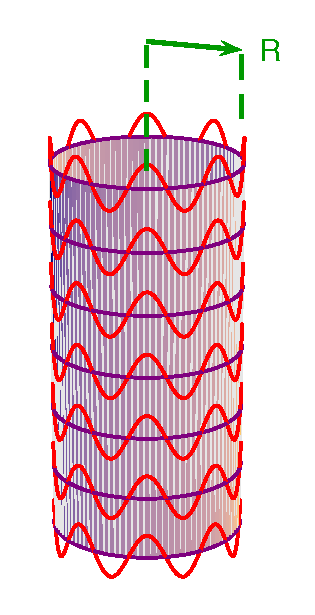
\includegraphics[width=0.2\textwidth]{figures/Theory/extradim.eps}
\captionsetup{width=0.85\textwidth} \caption{\small Representation of an extra spatial dimension with radius $R$. From reference \cite{Ponton:2012bi}.}
\label{sec:theo:fig:extradim}
\efig


\subsubsection{Flat-extra-dimensions models} 

In this category of models there are Arkani-Hamed-Dimopoulos-Dvali (ADD) models \cite{ArkaniHamed:1998rs} in which the extra dimension is accessible only to gravity; therefore, the only particle propagating in the bulk is the graviton. It requires two or more extra dimensions with a size $R$ that can range between $\sim1$ mm and $\sim1$ \tev$^{-1}$. The ``effective'' $4D$ Planck mass as a function of the $D$-dimensional parameters can be expressed as:
\be
M_{P}^{2}= M_{D}^{2+n}R^{n},
\ee
\noindent where $M_{D}$ is Planck scale in $D=4+n$ dimensions.  Fixing $M_{D}$ at around the electroweak scale to avoid introducing a new scale in the model, many options for the number and the size of the extra dimensions are possible. However, experimental lower bounds on the $M_{D}$ scale for ADD models are in the range of $4-6$ $\tev$ for $2-6$ extra dimensions \cite{Aaboud:2016tnv}, pushing $M_{D}$ away from the electroweak scale. \par
Allowing SM particles to propagate in the bulk is a feature of Universal Extra-Dimensional (UED) models \cite{Appelquist:2000nn}. The main challenge for these theories is recovering the SM behavior after compactification of the extra dimensions. One possibility is the existence of two extra dimensions, which are compactified under the real projective plane geometry (RPP) \cite{Burdman:2006gy,Cacciapaglia:2009pa}, referred to as 2UED/RPP model. In this case, new states can be produced only in pairs and the lightest KK state is stable, leading to a candidate for dark matter.

\subsubsection{Warped-extra-dimension models} 
\label{sec:theo:warped}

Randall and Sundrum (RS) \cite{Randall:1999vf,Contino:2006nn} models use a warped geometry in a five-dimensional Anti-de Sitter (AdS) spacetime with a compactification scale $\sim$\tev. The origin of the huge difference between the electroweak scale and the Planck scale is explained by the gravitational redshift factor present in the warped AdS metric. The ``warp'' factor determines how $4D$ scales change as a function of the position in the extra dimension:  energy scales for $4D$ fields localised on the infrared (IR) brane are red-shifted compared to the ones on the ultraviolet (UV) brane. Therefore, a natural solution to the hierarchy problem \cite{Randall:1999ee} can be achieved in this framework if the Higgs field is localised on the IR brane where the effective mass scales are of order \tev, while SM gauge bosons and fermions can propagate in the $5D$ bulk. In warped-extra-dimension models the Higgs boson appears as the fifth component of a $5D$ gauge boson and its mass is protected by the $5D$ gauge invariance.  In these models there is a light Higgs boson whose mass can be around 125 \gev, but it behaves as a composite pseudo-Nambu-Goldstone boson (see section \ref{sec:theo:compositeness}) with couplings that deviate from those of the SM Higgs boson.


\subsection{Compositeness}
\label{sec:theo:compositeness}

Several times a particle that was believed elementary revealed its composite nature when studied at higher energy scales, e.g. pions, protons and
even atoms were considered elementary at some point. Nowadays the idea that some of the SM particles may be composite is a fascinating  one, as the discovery of compositeness would radically redefine most of the fundamental questions in particle physics.\par
This idea developed starting from the not exact (i.e.~broken) chiral symmetry in QCD, which produces three Goldstone bosons with a mass, usually referred to as pseudo-Nambu-Goldstone Bosons (PNGB). The three PNGBs are the pions, which are not elementary particles and have a naturally low mass compared to other mesons. Before it was established as a meson, i.e. a quark-antiquark bound state of the strong interaction, the neutral pion was considered an elementary
particle, responsible for mediating the strong interaction. The low mass ($\sim$100 \mev) of the neutral pion could, however, not be explained without interpreting it as a meson. This in turn required new particles at the $\gev$ scale, which were indeed found thereafter. This is the result of strong dynamics that can be reinterpreted in terms of more fundamental degrees of freedom, the quarks.\par
Some new theories propose that the Higgs boson is a composite PNGB \cite{Agashe:2004rs,Kaplan1984187,Fukano:2013aea,Contino:2010rs}. In these theories, a new strongly-interacting sector with a new global symmetry is present at the compositeness scale, usually $\sim\tev$. A composite light Higgs boson emerges, much like the pion of QCD, as the PNGB of a global symmetry breaking of that sector. The explicit symmetry breaking is induced by interactions of the SM gauge bosons and fermions with the strong sector. Loops of SM fermions and gauge bosons generate a Higgs potential that eventually breaks the electroweak symmetry at scale $v$, generated dynamically and lower than the strong sector (compositeness) breaking scale. In this scenario the radiative corrections to the Higgs boson mass do not reach the Planck scale since the Higgs boson will reveal its composite nature at the energy scale of the new strong sector. Strongly-interacting theories usually are subject to stringent constraints from precision electroweak data, but weakly-coupled models such as the one in section \ref{sec:theo:warped} can satisfy such bounds. \par
Some other theories propose instead that the top quark is composite \cite{Pomarol:2008bh}, made of some new constituent particles (``preons'') bound together by a new confining force, or a condensed state. Most of those models \cite{Lillie:2007hd,Kumar:2009vs} focus on right-handed top quarks to avoid strong constraints from precision electroweak data.\\


\subsection{Vector-like quarks}
\label{sec:theo:vlq}

A fermion is vector-like if  left- and right-handed chiralities belong to the same representation of the symmetry group of the underlying theory.
Vector-like quarks (VLQs) are triplets under the $SU(3)_{C}$ gauge group, and so their left- and right-handed components carry the same colour and electroweak quantum numbers \cite{Aguilar-Saavedra:2013qpa,Okada:2012gy,Aguilar-Saavedra:2013wba,jaas}. VLQs have been introduced in many different BSM scenarios; in composite Higgs models VLQs are part of the condensate that drives the EW symmetry breaking, the excited partners of SM quarks in extra-dimensional models are also vector-like. The presence of VLQs can introduce new sources of CP violation to solve the baryon asymmetry \cite{delAguila:1997vn} and can also explain the observed $A^{b}_{FB}$ asymmetry through mixing with the bottom quark \cite{Choudhury:2001hs,Kumar:2010vx}. The introduction of VLQs also stabilises the Higgs boson mass since the quadratic divergences cancel and only a logarithmic divergence remains. The one-loop contributions to the Higgs boson mass are shown in figure \ref{fig:theo:VLQHiggsmass}. 

\begin{figure}[h!]
\begin{subfigure}{0.33\textwidth}
  \centering
  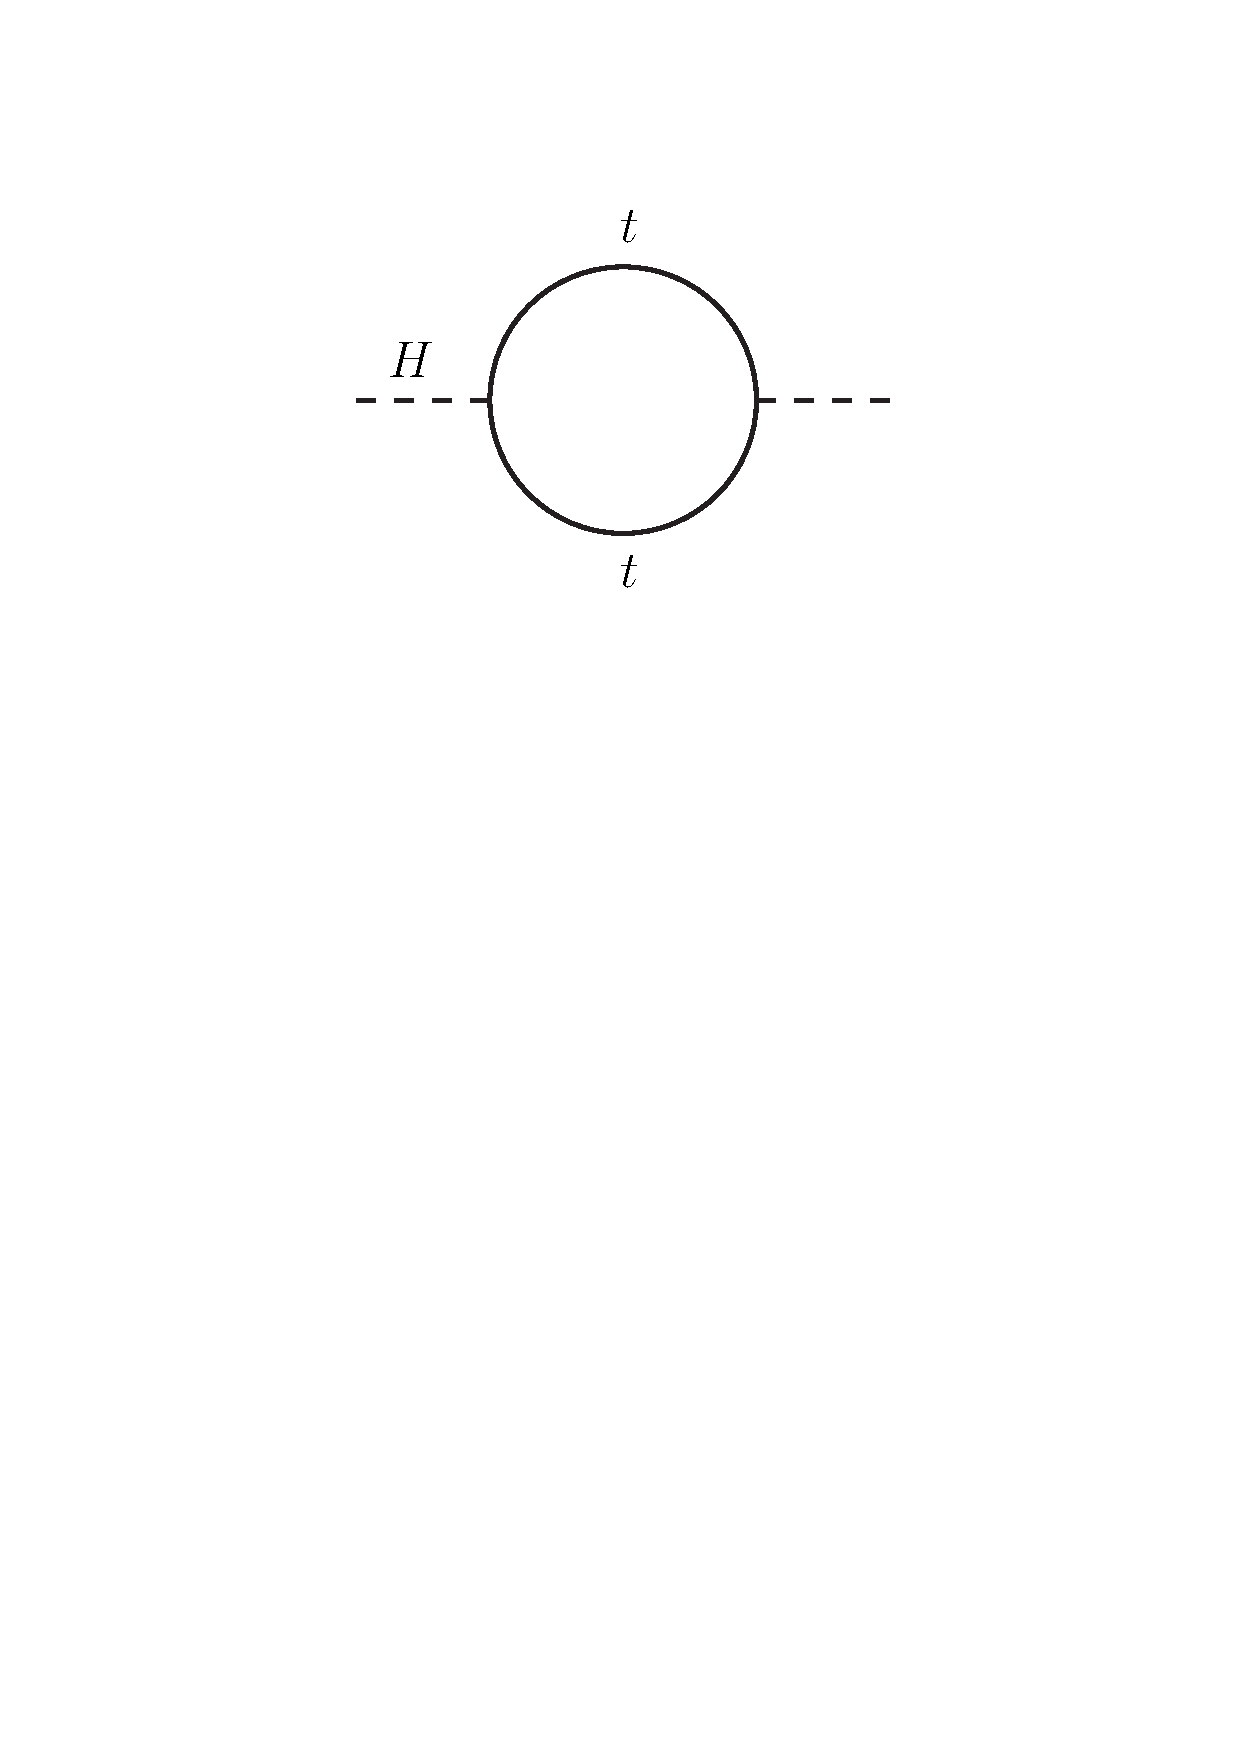
\includegraphics[width=0.9\textwidth]{figures/Theory/loop_toptop_good.pdf}
  \caption{}
  \label{}
\end{subfigure}
\begin{subfigure}{0.33\textwidth}
  \centering
  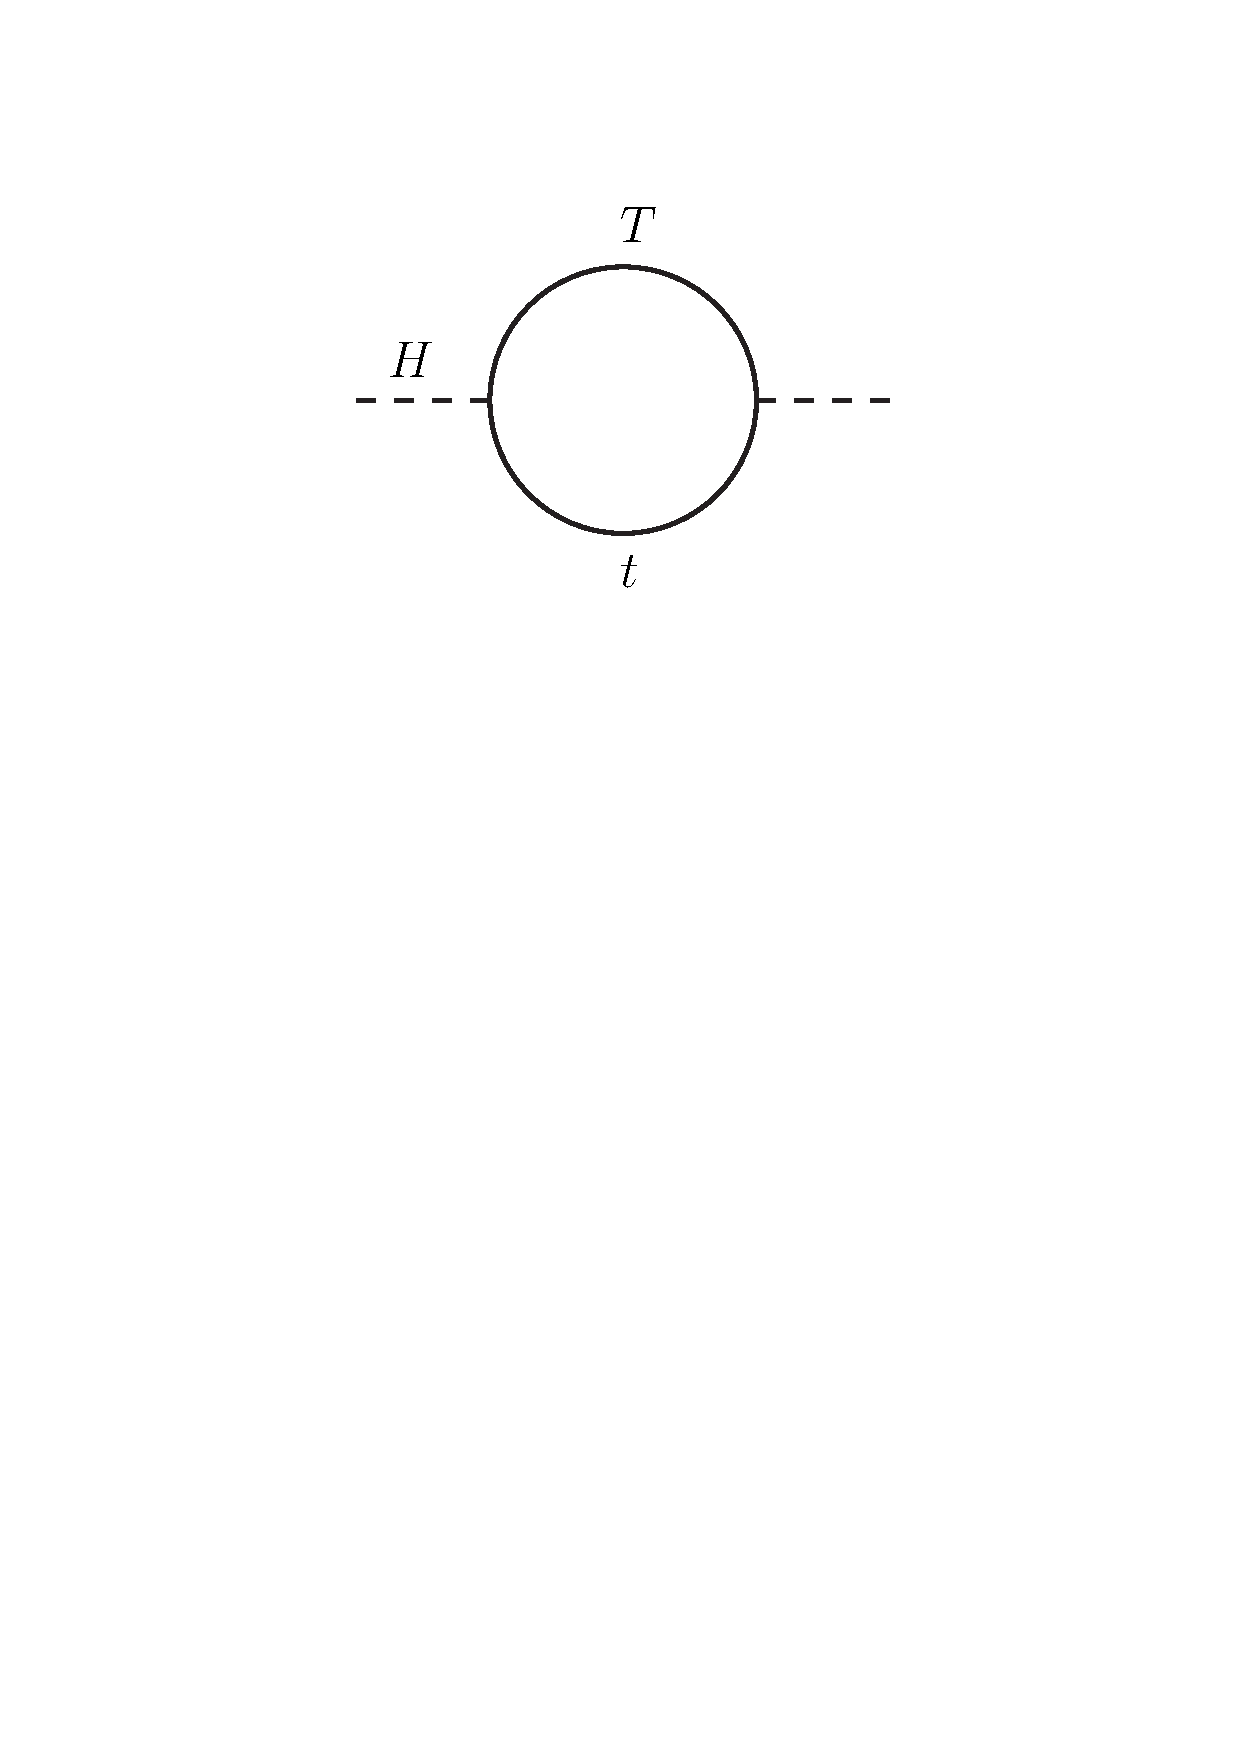
\includegraphics[width=0.9\textwidth]{figures/Theory/loop_topT_good.pdf}
  \caption{}
  \label{}
\end{subfigure}
\begin{subfigure}{0.33\textwidth}
  \centering
  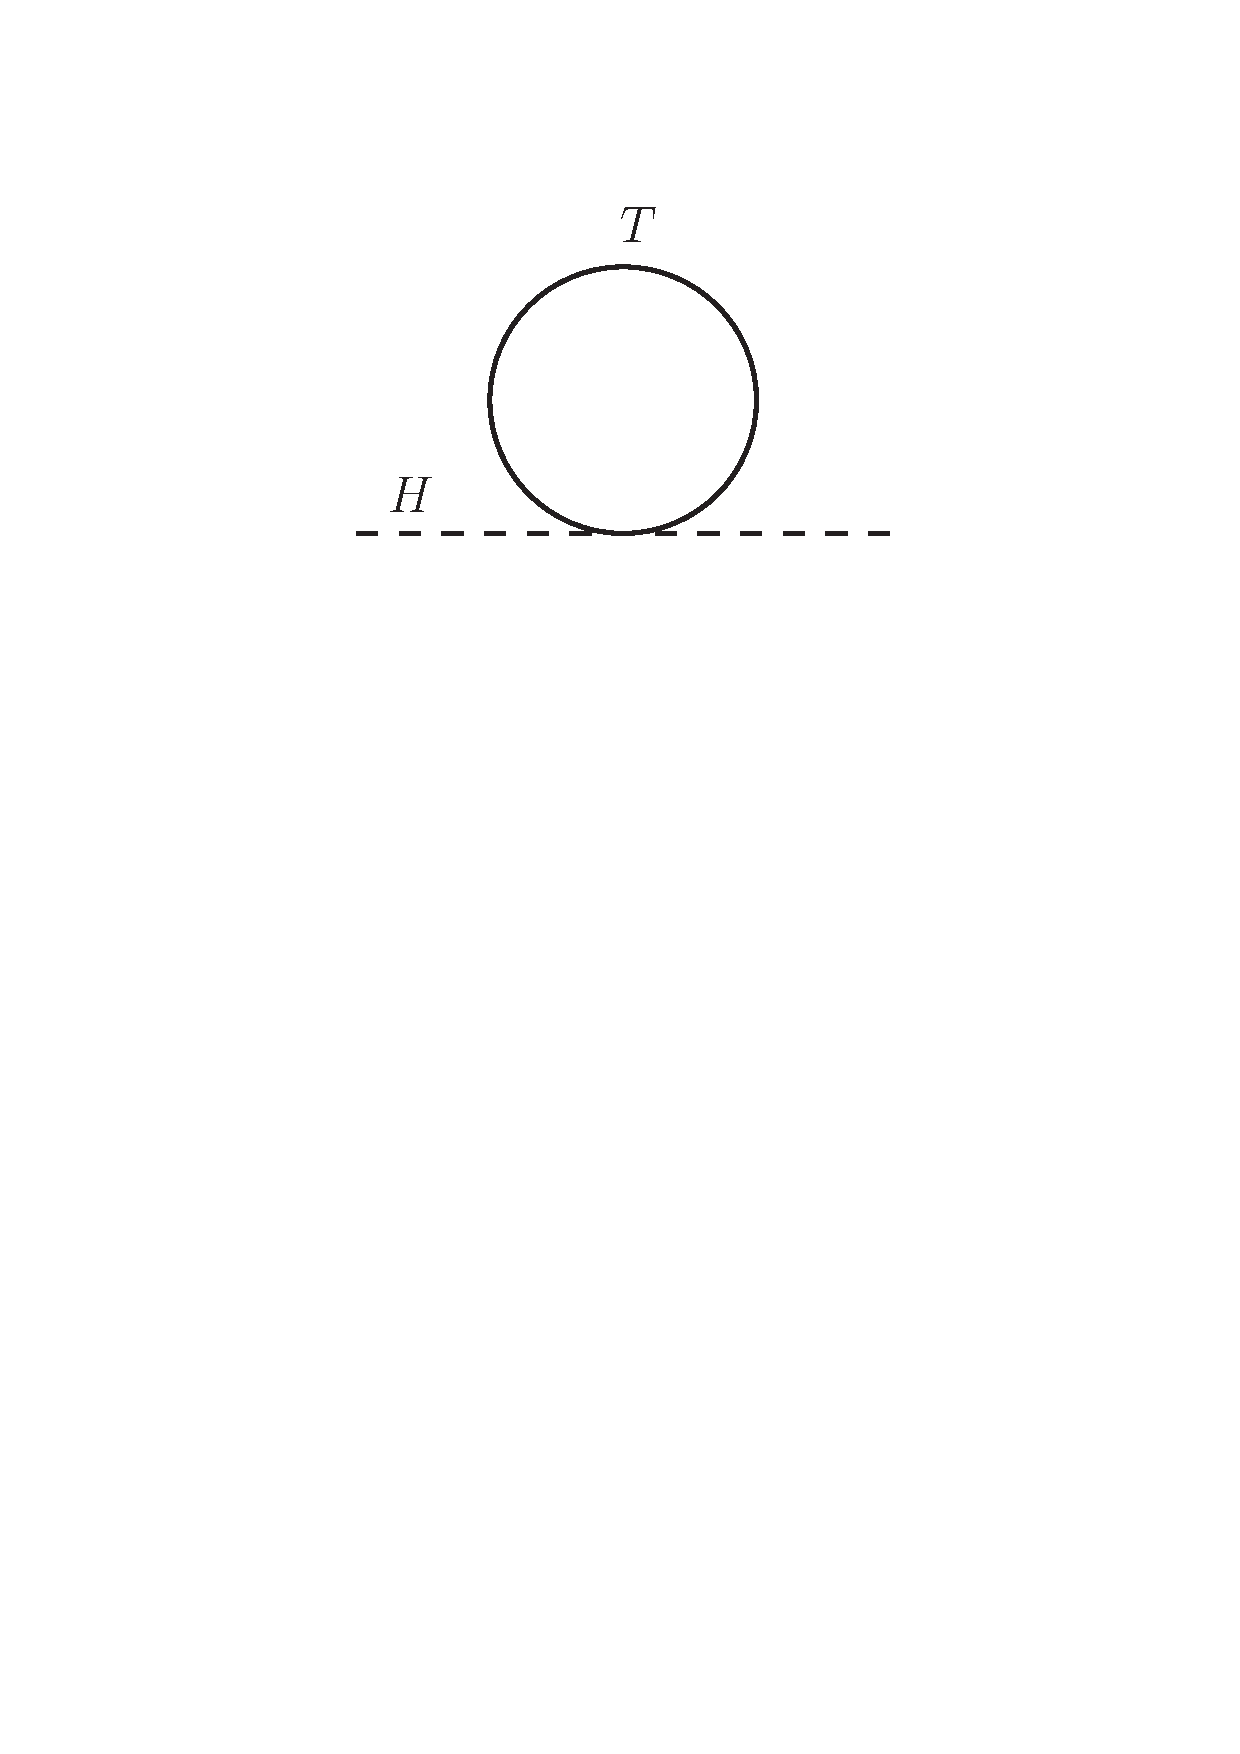
\includegraphics[width=0.9\textwidth]{figures/Theory/loop_T_good.pdf}
  \caption{}
  \label{}
\end{subfigure}

\captionsetup{width=0.85\textwidth} \caption{\small One-loop contributions to the Higgs boson mass term from (a) the top quark and (b, c) a vector-like top-quark partner $T$.}
\label{fig:theo:VLQHiggsmass}
\end{figure}

The mass term $m_{f}\bar{\Psi}_{f}\Psi_{f}$ of a VLQ $f$ is gauge invariant under $SU(2)_{L} \otimes U(1)_{Y}$, i.e. its mass is generated without the need for a Yukawa interaction with the Higgs boson. Therefore, there are no constraints on the existence of VLQs arising from the measured Higgs-boson production cross section, since the contribution to loop-induced Higgs-boson couplings, $ggH$ and $\gamma\gamma H$, is suppressed by the heavy quark mass.
Classifying VLQs in multiplets of $SU(2)_{L}$, it is possible to write gauge-invariant interaction terms only for singlets, doublets and triplet representations, shown in table \ref{sec:theo:vlqs}. 

\begin{table}[htb]
\begin{eqnarray*}
\setlength{\arraycolsep}{2pt}
\begin{array}{cccccccc}
&\multicolumn{2}{c}{\mbox{Singlets}}&\multicolumn{3}{c}{\mbox{Doublets}}&\multicolumn{2}{c}{\mbox{Triplets}}\\
& 
\begin{array}{c} ~ \\ (U) \\ ~ \\ ~ \end{array} &
\begin{array}{c} ~ \\ ~ \\ (D) \\ ~ \end{array} & 
\begin{array}{c} \left(\begin{array}{c} X \\ U \end{array}\right) \\ ~ \\ ~ \end{array} &
\begin{array}{c} ~ \\ \left(\begin{array}{c} U \\ D \end{array}\right) \\ ~ \end{array} &
\begin{array}{c} ~ \\ ~ \\ \left(\begin{array}{c} D \\ Y \end{array}\right) \end{array} & 
\begin{array}{c} \left(\begin{array}{c} X \\ U \\ D \end{array}\right) \\ ~ \end{array} &
\begin{array}{c} ~ \\ \left(\begin{array}{c} U \\ D \\ Y \end{array}\right) \end{array} \\
\midrule
Y/2  & 2/3 & -1/3 & 7/6 & 1/6 & -5/6 & 2/3 & -1/3 \\
\midrule
\mathcal{L}_{\rm Yukawa} &
\multicolumn{2}{c}{\begin{array}{c}-\lambda_u^i \bar q_L^i H^c U_R \\-\lambda_d^i \bar q_L^i H D_R \end{array}} &
\multicolumn{3}{c}{\begin{array}{c}-\lambda_u^i \psi_L H^{(c)} u_R^i \\-\lambda_d^i \psi_L H^{(c)} d_R^i \end{array}} &
\multicolumn{2}{c}{\begin{array}{c}-\lambda_i \bar q_L^i \tau^a H^{(c)} \psi_R^a \end{array}} \\
\midrule

\end{array} 
\end{eqnarray*}
\captionsetup{width=0.85\textwidth} \caption{\small VLQs in different $SU(2)_L$ representations with hypercharge quantum number and Yukawa mixing terms in the Lagrangian. Depending on the chosen representation, the Higgs boson may be $H$ or $H^c$; therefore, it has been noted as $H^{(c)}$ when necessary.}
\label{sec:theo:vlqs}
\end{table}


The mass eigenstates are labelled as $X$, $T$, $B$, and $Y$ with an electric charge of $+5/3$, $+2/3$, $-1/3$, $-4/3$ respectively.
The left-right symmetry of VLQs allows for tree-level flavour changing neutral currents, which are their distinctive feature.  In order to be consistent with precision electroweak data, a small mass splitting between VLQs belonging to the same $SU(2)_{L}$ multiplet is required \cite{Aguilar-Saavedra:2013qpa}, which forbids cascade decays such as $T \to WB$, and leaves direct decays into SM particles as the only possibility. VLQs interact with SM quarks and the Higgs boson through Yukawa couplings. VLQs can mix with the SM quarks; the mixing occurs in the left-handed sector for the singlet and triplet representations and in the right-handed sector for the doublet representation. The mixing of a VLQ and a SM quark is of the order $\sim m_{q}/M_{Q}$, where $M$ and $m$ are the masses of the VLQ and the SM quark respectively. Thus VLQs are expected to predominantly mix with the third SM generation, while mixing with lighter SM generations is mass suppressed. Under this assumption, the only possible decays for VLQs are into top / bottom quark plus a $W$, $Z$ or Higgs boson. For the quarks with exotic charges the only decay channels are $X \to W^{+}t$ and $Y\to W^{-}b$, while the heavy quarks  with charges $+2/3$ and $-1/3$ the possible channels are respectively:

\be
T\to W^{+}b,\, Zt,\, Ht \,\,\,\, \textrm{and} \,\,\,\, B\to W^{-}t,\, Zb,\, Hb.
\ee

\noindent The branching ratios for different channels have some dependence on the heavy quark masses and on the $SU(2)_{L}$ representation. For singlets all decay modes are possible, while for doublets the branching ratio depend on the relative size of the mixing factors $V_{Tb}$ and $V_{tB}$ of the extended CKM matrix. In this dissertation the scenario where $V_{Tb} \ll V_{tB}$ is assumed. Thus the mixing of the heavy quarks with the SM top quark is much stronger, and the $T\to Wb$ decay is suppressed, as well as $B\to Hb$ and $B\to Zb$. Table \ref{sec:theo:tab:VLQ_decay} summarises the possible decays modes for VLQs.
\begin{table}[htb!]
   \centering
   \begin{tabular}{ccc}
   \begin{tabular}{cc}
     \toprule
     \toprule
     Singlets & Decay modes \\
     \midrule
     & \\
     $X$ & $W^+t$ \\
     & \\
     $T$ & $W^+b,\, Ht,\, Zt$ \\
     & \\
     $B$ & $ W^-t,\, Hb,\, Zb$ \\
     & \\
     $Y$ & $W^-b$ \\
     & \\
     & \\%one empty line
     \bottomrule
     \bottomrule
   \end{tabular}

   & 

   \begin{tabular}{cc}
     \toprule
     \toprule
      Doublets & Decay modes\\
     \midrule
     &\\%one empty line
     \multirow{2}{*}{$\left(\begin{array}{c}X \\ T\end{array}\right)$} & $W^+t$\\
     & $Ht,\, Zt$\\
     &\\
     \multirow{2}{*}{$\left(\begin{array}{c}T \\ B\end{array}\right)$} & $ Ht,\, Zt$ \\%$W^+b,\, Ht,\, Zt$\\
     & $ W^-t$\\%$ W^-t,\, Hb,\, Zb$\\
     & \\
     \multirow{2}{*}{$\left(\begin{array}{c}B \\ Y\end{array}\right)$} & $Hb,\, Zb$\\
     & $W^-b$\\
     &\\%one empty line
     \bottomrule
     \bottomrule
   \end{tabular}
   & 

   \begin{tabular}{cc}
     \toprule
     \toprule
      Triplets & Decay modes\\
     \midrule
     &\\%one empty line
     \multirow{3}{*}{$\left(\begin{array}{c}X \\ T \\ B\end{array}\right)$} & $ W^+t$ \\
     & $W^+b,\, Ht,\ Zt$\\
     & $Hb,\, Zb$\\
     &\\%one empty line
     \multirow{3}{*}{$\left(\begin{array}{c}T \\ B \\ Y\end{array}\right)$} & $Ht,\, Zt$\\
     & $W^-t,\, Hb,\, Zb$\\
     & $W^-b$\\
     &\\%one empty line
     &\\%one empty line
     \bottomrule
     \bottomrule
   \end{tabular}
   \end{tabular}
   \captionsetup{width=0.85\textwidth} \caption{\small Allowed decay modes for vector-like singlets, doublets and triplets.}
     \label{sec:theo:tab:VLQ_decay}
   \end{table}
Figure \ref{fig:theo:VLQBRs} shows the decay branching ratios of the vector-like top and bottom partners for singlets and doublets as a function of the heavy-quark mass.
  
\begin{figure}[t!]
\begin{subfigure}{0.5\textwidth}
  \centering
  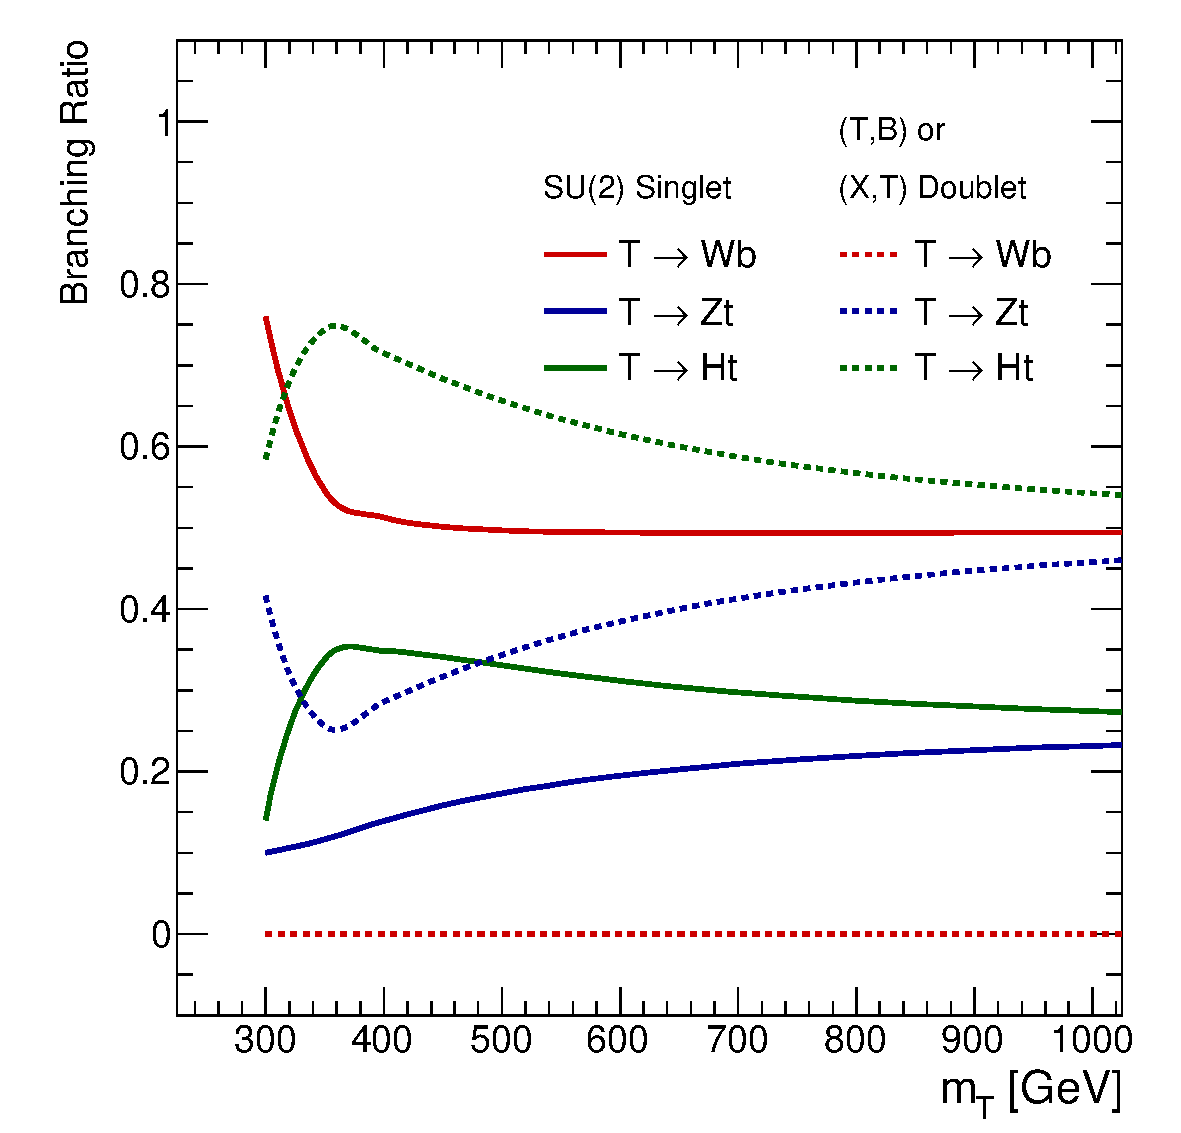
\includegraphics[width=0.9\textwidth]{figures/Theory/fig_02a.png}
  \caption{}
  \label{}
\end{subfigure}
\begin{subfigure}{0.5\textwidth}
  \centering
  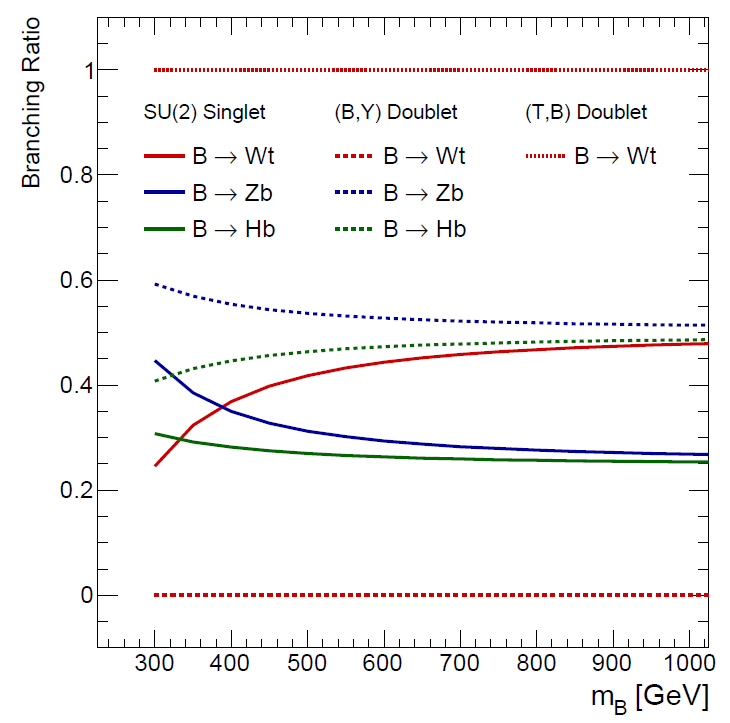
\includegraphics[width=0.9\textwidth]{figures/Theory/fig_02b.png}
  \caption{}
  \label{}
\end{subfigure}

\captionsetup{width=0.85\textwidth} \caption{\small Branching ratios for vector-like (a) top and (b) bottom partners as function of the heavy-quark mass $m_{T}$ and $m_{B}$ respectively for singlets and doublets. From reference \cite{Aguilar-Saavedra:2013qpa}.}
\label{fig:theo:VLQBRs}
\end{figure}

VLQs can be produced either in pairs through the strong interaction or as single quarks in association with SM quarks or bosons through the weak interaction \cite{Buchkremer:2013bha}.
Pair production is model independent since it just depends on the VLQ mass, while single production depends on the strength of VLQ coupling to SM quarks, and thus is model dependent. However, pair production suffers from a larger phase-space suppression with respect to single production, and if the VLQ mass is large enough ($\sim \tev$), single production may dominate over pair production. Example Feynman diagrams for pair and single production of a vector-like $T$-quark are shown in figure \ref{fig:theo:VLQprod}. Figure \ref{sec:theo:fig:vlqxsec} shows the cross section for pair production and single production in the $t$-channel as a function of VLQ mass.
\begin{figure}[h!]
\begin{subfigure}{0.5\textwidth}
  \centering
  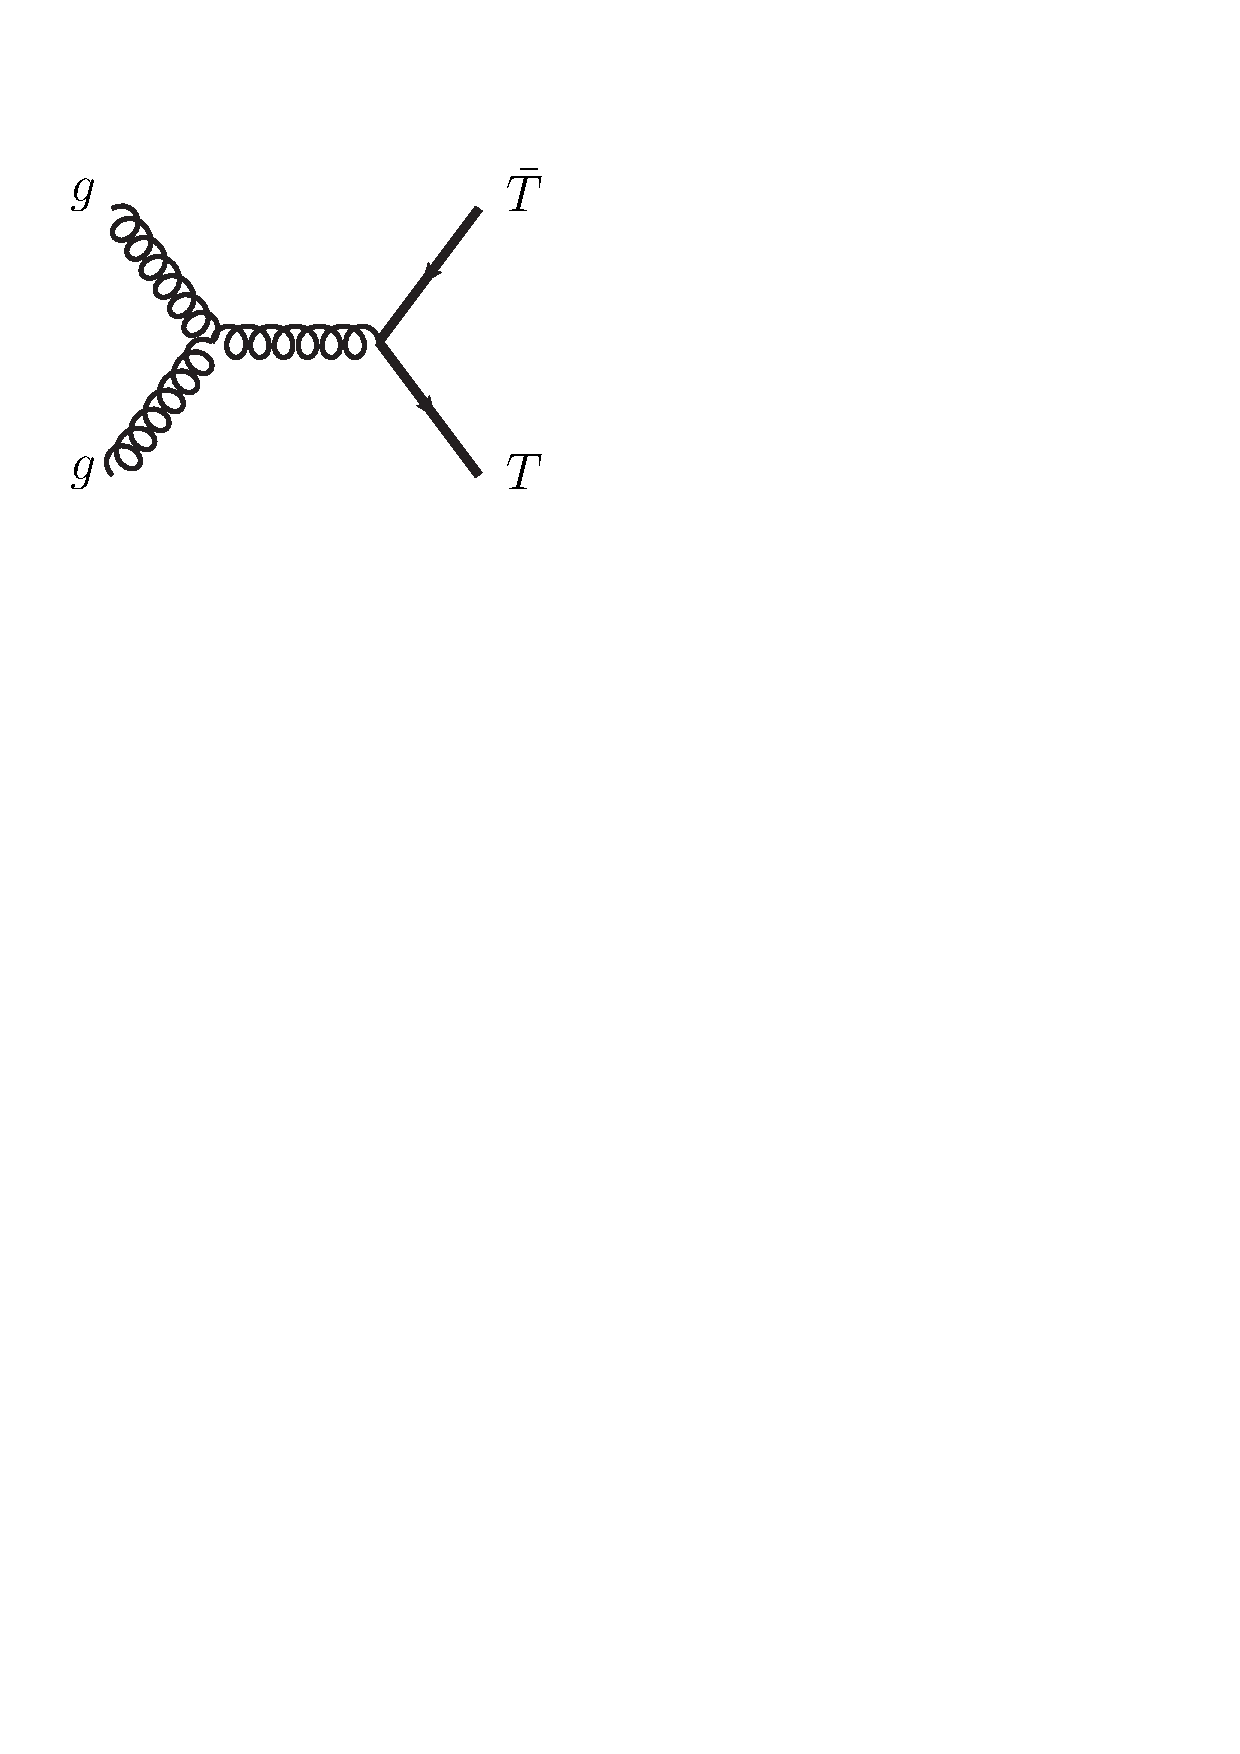
\includegraphics[width=0.6\textwidth]{figures/Theory/T_pairProd_good.pdf}
  \caption{}
  \label{}
\end{subfigure}
\begin{subfigure}{0.5\textwidth}
  \centering
  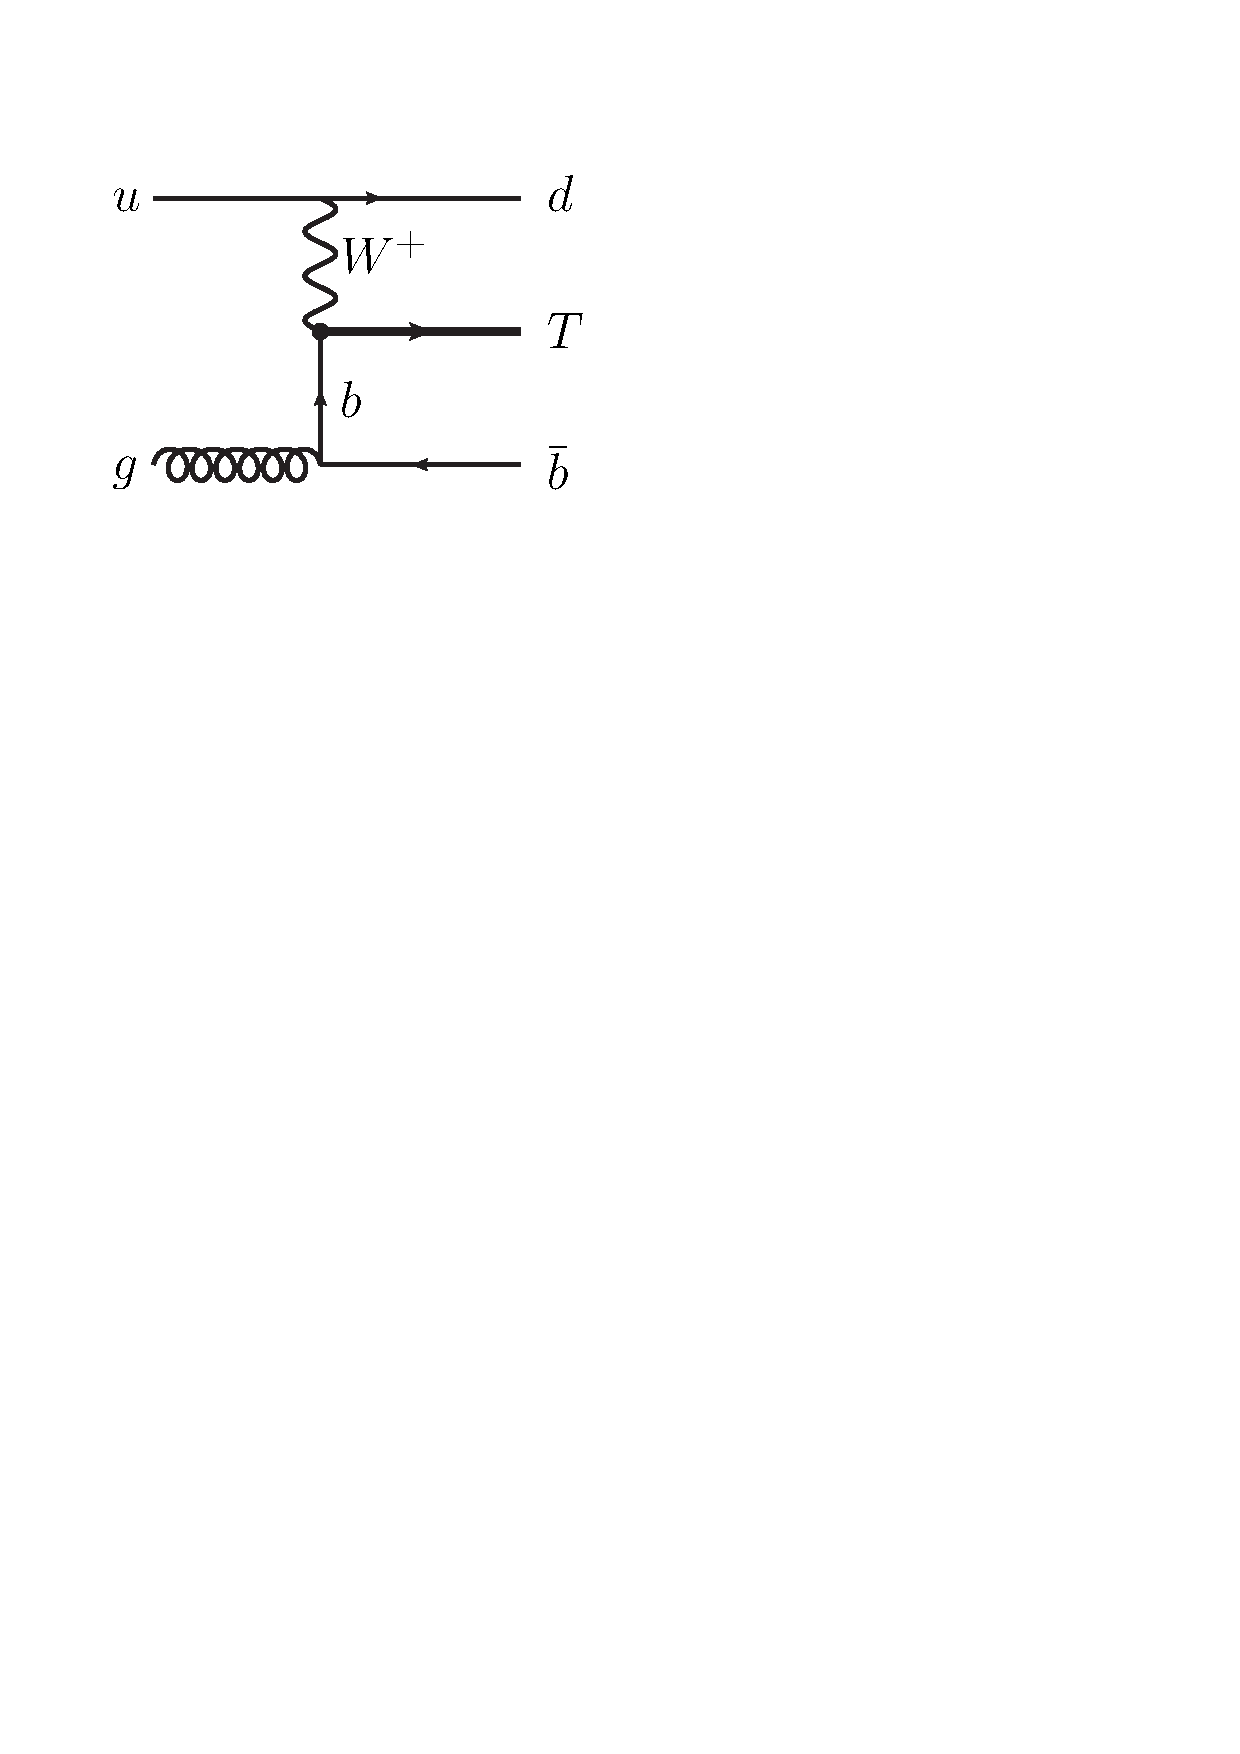
\includegraphics[width=0.6\textwidth]{figures/Theory/T_singleProd_good.pdf}
  \caption{}
  \label{}
\end{subfigure}

\captionsetup{width=0.85\textwidth} \caption{\small Representative leading-order Feynman diagrams for vector-like top (a) pair-production and (b) single-production modes.}
\label{fig:theo:VLQprod}
\end{figure}


\bfig[h!]
\centering
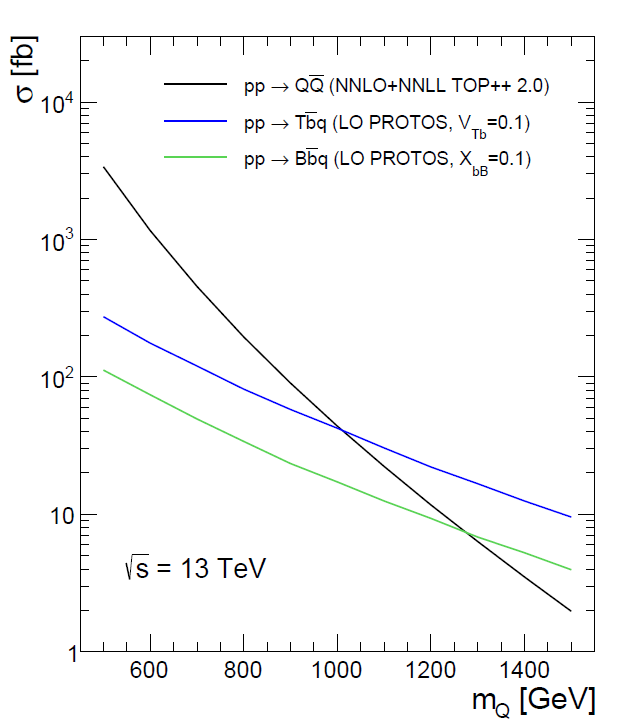
\includegraphics[width=0.4\textwidth]{figures/Theory/VLQxsec.png}
\captionsetup{width=0.85\textwidth} \caption{\small Production cross sections for pair and single production of VLQs in $pp$ collisions at $\sqrt{s}=$13 \tev. Pair production is computed at NNLO+NNLL order in QCD using {\sc Top++} 2.0 while single production is computed at LO in QCD with {\sc Protos} assuming $V_{Tb}=0.1$ and $X_{bB}=0.1$.}
\label{sec:theo:fig:vlqxsec}
\efig


\subsection{Anomalous four-top-quark production}
\label{sec:theo:fourtops}

The cross section of four-top-quark events predicted by the SM (see figure \ref{fig:theo:fourtopSM}) is extremely small, $\sigma_{t\bar{t}t\bar{t}}=9.2$ fb at $\sqrt{s} = 13$ $\tev$ \cite{Barger:1991vn}. 
However, in many BSM models, the four-top-quark production is enhanced, usually through the pair production of a new particle decaying to a top-antitop pair.\par
For example, a possible source of enhancement of the $t\bar{t}t\bar{t}$ cross-section appears in extra-dimensional models. In this framework the four-top-quark signal is an important probe for low-scale warped extra dimensions \cite{Jung:2010ms}; the enhancement comes from a heavy gluon that can be pair produced and decay into $\ttbar$ or via associate production of the heavy gluon with $t\bar{t}$. In flat-extra-dimensions models, such as 2UED/RPP, the enhancement is caused by the lightest particle of the tier (1,1), i.e. the vector photon $A_{\mu}^{(1,1)}$. In these models, to each SM fields corresponds a tower of massive resonances organised in tiers, labelled by two integers ($\ell$, $k$) that correspond to the discretised momenta along the extra dimensions. At leading order, all the states in each tier are degenerate with mass determined by the two integers:
\be
m^{2}=\frac{\ell^{2}}{R^{2}_{5}}+\frac{k^{2}}{R^{2}_{6}},
\ee 
\noindent where $R_{5}$ and $R_{6}$ are respectively the size of the two extra dimensions. For tier (1,1) its mass is given by $M^{(1,1)}=\sqrt{1/R^{2}_{5}+1/R^{2}_{5}}\sim \sqrt{2}M_{KK}$; assuming the two extra dimensions have the same size, and where $M_{KK}=M^{(0,1)}=M^{(1,0)}$.
The production of any heavy state of tier (1,1) contributes to the production of vector photons since it will undergo chain decays until the lightest state\footnote{The SM particles radiated in the chain decay are soft due to the typically small mass differences between states in the tier, and therefore will easily escape detection.} (see figure \ref{fig:theo:fourtopUED}). Therefore, the production cross section of vector photons can be sizeable even though their couplings to quarks and gluons are small.
The branching ratios of $A_{\mu}^{(1,1)}$ into SM particles are not predicted by the model, although the decay into $t\bar{t}$ is expected to be dominant \cite{Cacciapaglia:2011kz}.\par It is also possible to parametrise new physics, maybe not accessible at LHC, leading to four-top-quark production using the language of effective field theory with higher-dimensional operators.  This approach is used by composite top quark scenarios or RS models, in which, below the new physics scale, phenomena are described by an effective field theory containing the bound states of the new sector.
A dimension-six Lorentz-invariant operator with a four-point interaction (see figure \ref{fig:theo:fourtopEFT}) that involves only right-handed top quarks, $t_{R}$, can be considered:

\be
\mathcal{L}_{4t}=\frac{C_{4t}}{\Lambda^{2}}(\bar{t_{R}}\gamma_{\mu}t_{R})(\bar{t_{R}}\gamma_{\mu}t_{R}),
\ee 

\noindent where $\Lambda$ is the scale where new physics will manifest, and $C_{4t}$ is the effective coupling. The effective field theory approach is valid for $|C_{4t}|<16\pi^{2}$. In this framework right-handed top quarks are chosen because of the strong constraints coming from precision electroweak data on operators involving left-handed top quarks. 

\begin{figure}[t!]
\begin{subfigure}{0.33\textwidth}
  \centering
  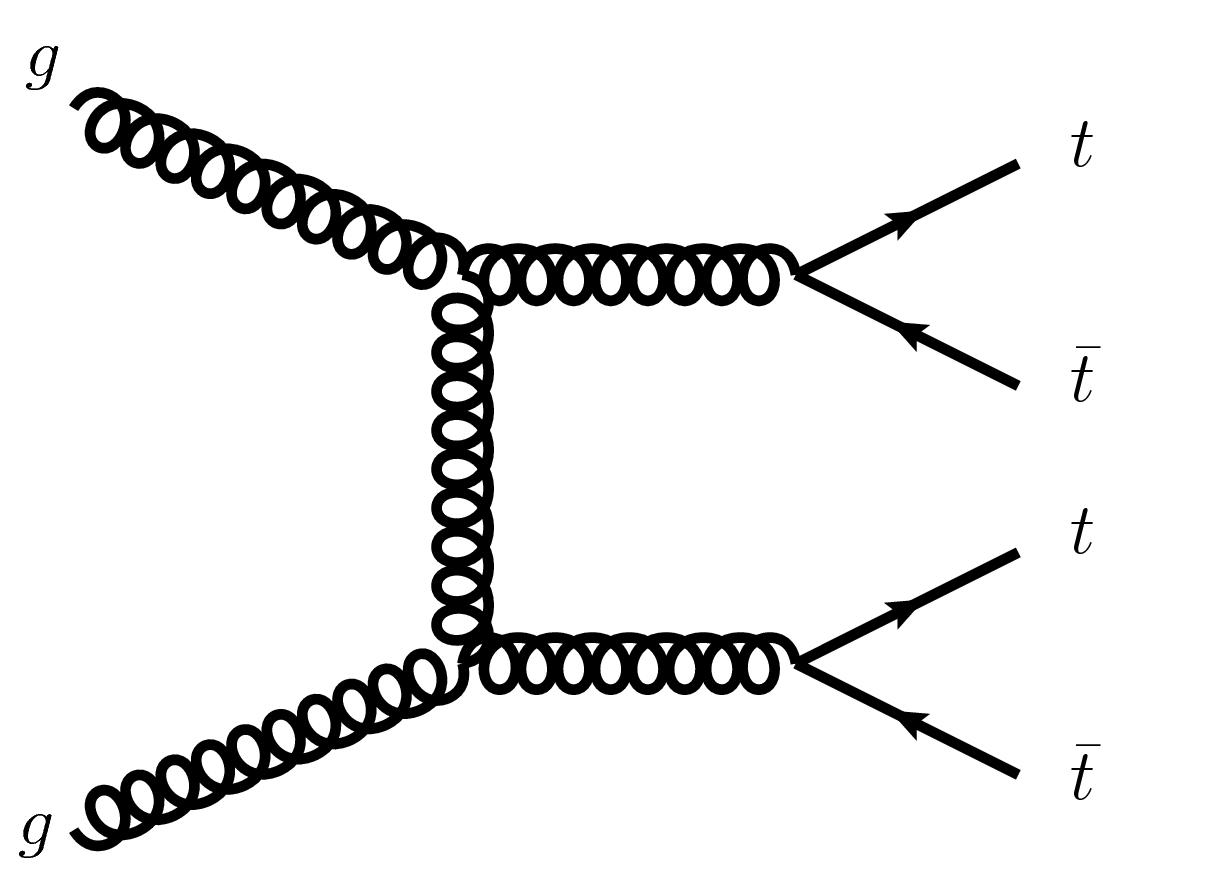
\includegraphics[width=0.8\textwidth]{figures/Theory/fig_03a.png}
  \caption{}
  \label{fig:theo:fourtopSM}
\end{subfigure}
\begin{subfigure}{0.33\textwidth}
  \centering
  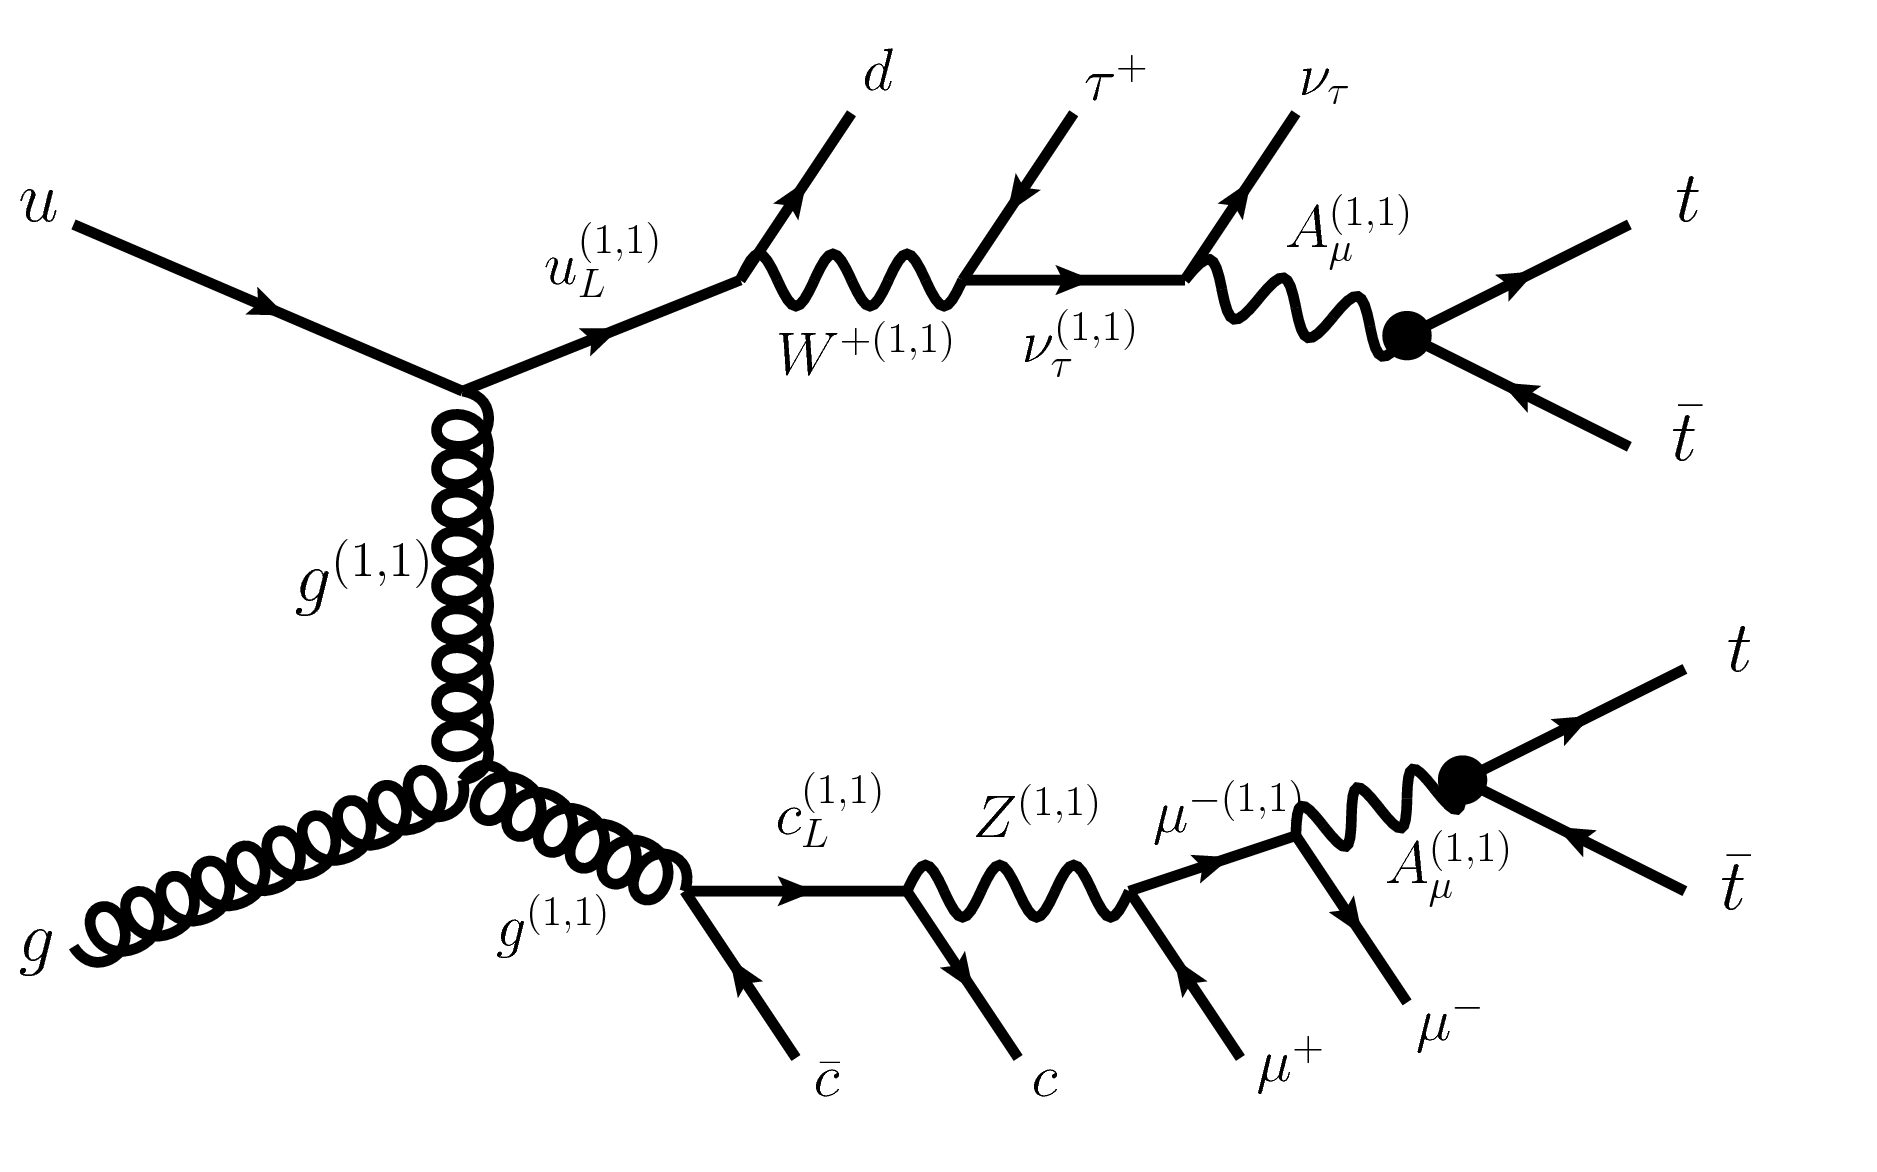
\includegraphics[width=1.15\textwidth]{figures/Theory/fig_03c.png}
  \caption{}
  \label{fig:theo:fourtopUED}
\end{subfigure}
\begin{subfigure}{0.33\textwidth}
  \centering
  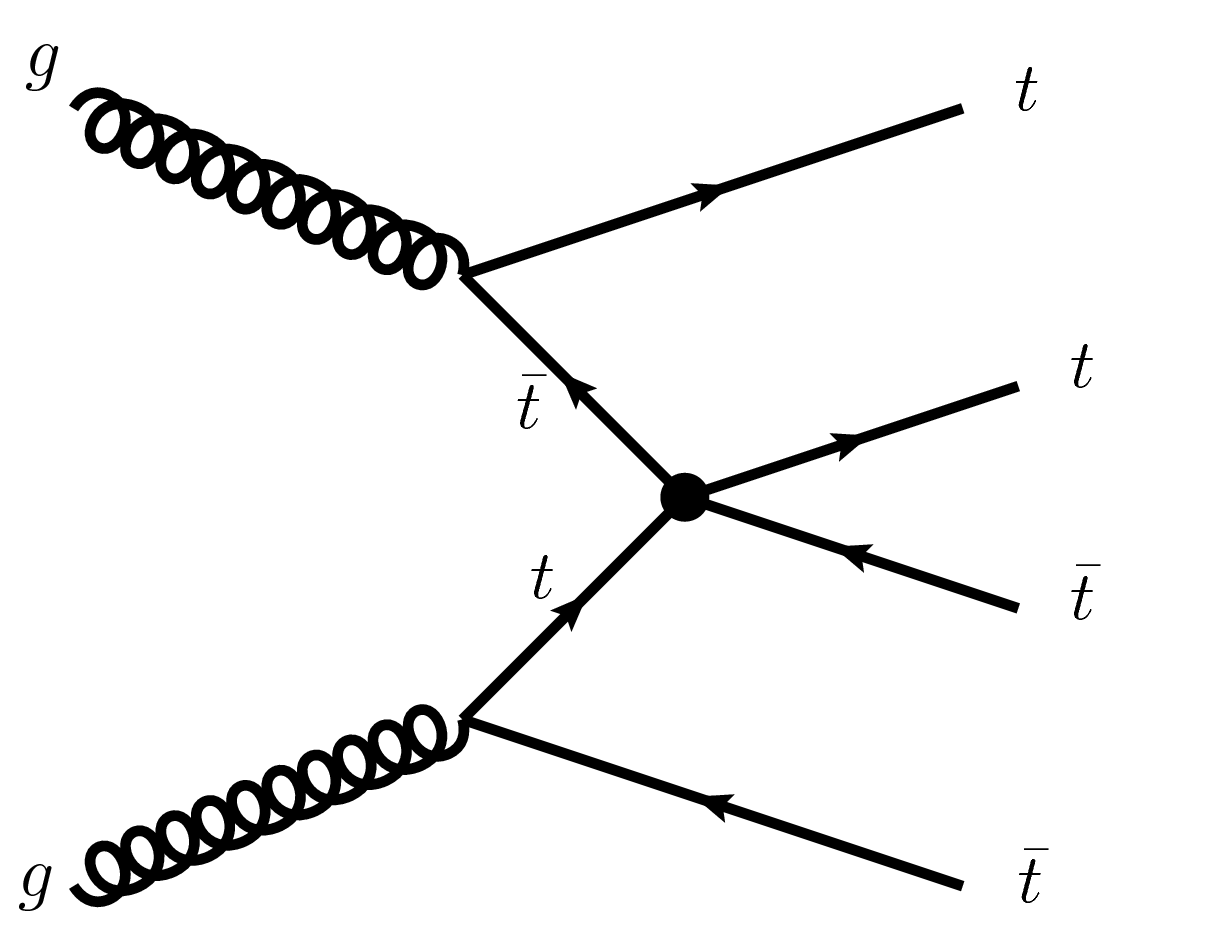
\includegraphics[width=0.75\textwidth]{figures/Theory/fig_03b.png}
  \caption{}
  \label{fig:theo:fourtopEFT}
\end{subfigure}


\captionsetup{width=0.85\textwidth} \caption{\small Representative leading-order Feynman diagrams for four-top-quark production within (a) the SM and several BSM scenarios: (b) via cascade decays from Kaluza-Klein excitations in a universal extra dimensions model with two extra dimensions compactified using the geometry of the real projective plane, and (c) via an effective four-top-quark interaction in an effective field theory model.}
\label{fig:theo:fourtop}
\end{figure}

	
	\chapter{The ATLAS experiment at the Large Hadron Collider}
\label{chp:det}

\begin{flushright}
\begin{small}
\emph{Nos esse quasi nanos gigantium humeris insidentes}.\\Bernardus Carnotensis
\end{small}
\end{flushright}

\minitoc

\label{chp:det:intro}
Exploring the $\tev$ energy scale requires particle accelerators and the corresponding experiments to be designed and built for this purpose. The first part of this chapter describes the world's largest and most powerful particle accelerator, the Large Hadron Collider (LHC), with a particular emphasis on the evolution of the running parameters over the past years of operation. The second part of this chapter is focused on the ATLAS detector, one of the four large experiments studying the high-energy collisions produced by the LHC. An overview of its subdetector components and their performance is also provided.\\
 

\section{The Large Hadron Collider}
\label{chp:det:LHC}

The LHC \cite{Evans:2008zzb} is a circular proton-proton collider located at the European Council for Nuclear Research (CERN). The machine is hosted in a 27 km circumference tunnel built between 50 m and 170 m underneath the French-Swiss countryside outside Geneva. Not only it is the world's largest collider but, with the current operation at a beam energy of 6.5 $\tev$ and its expected upgrade to the design energy of 7 $\tev$, it is also the most powerful.  It was designed to extend the reach of previous accelerators in the study of SM processes and searches for new phenomena.\par
The centre-of-mass energy increased by about a factor of seven with respect to the Tevatron collider at Fermilab \cite{fermilab}, while the high instantaneous luminosity (up to $10^{34}$ cm$^{-2}$s$^{-1}$) allows access to very rare processes and precision measurements. These considerations ultimately motivated the choice of a proton-proton collider. For protons the energy loss in a curved trajectory due to synchrotron radiation\footnote{The energy emission per turn is proportional to $(E/m)^{4}$, where $E$ and $m$ are the energy and mass of the particle respectively.}  is considerably smaller than for electrons and this allows accelerating protons more efficiently in a circular machine. At the same time, a hadron collider probes multiple energy scales simultaneously due to the momentum distribution of partons inside the protons.  A proton-antiproton collider alternative was rejected due to the difficulties of producing and operating high-intensity antiproton beams, which would have resulted in a lower peak luminosity. The LHC is also able to accelerate and collide lead ions at the nominal energy of 2.76 $\tev$/nucleon, for a total centre-of-mass energy of 1.15 $\pev$.

\subsection{CERN accelerator complex}

As for any other large particle collider, the energy of the colliding particles is gradually increased by subsequent acceleration steps; this solution has high flexibility and allows for a more efficient beam production. At the same time, intermediate accelerator machines provide beams that are used in other lower-energy experiments. A sequence of accelerators, shown in figure \ref{sec:det:fig:acccomplex}, is involved in the preacceleration of the protons before they are injected into the LHC ring \cite{Benedikt:2004wm}.

\bfig[h!]
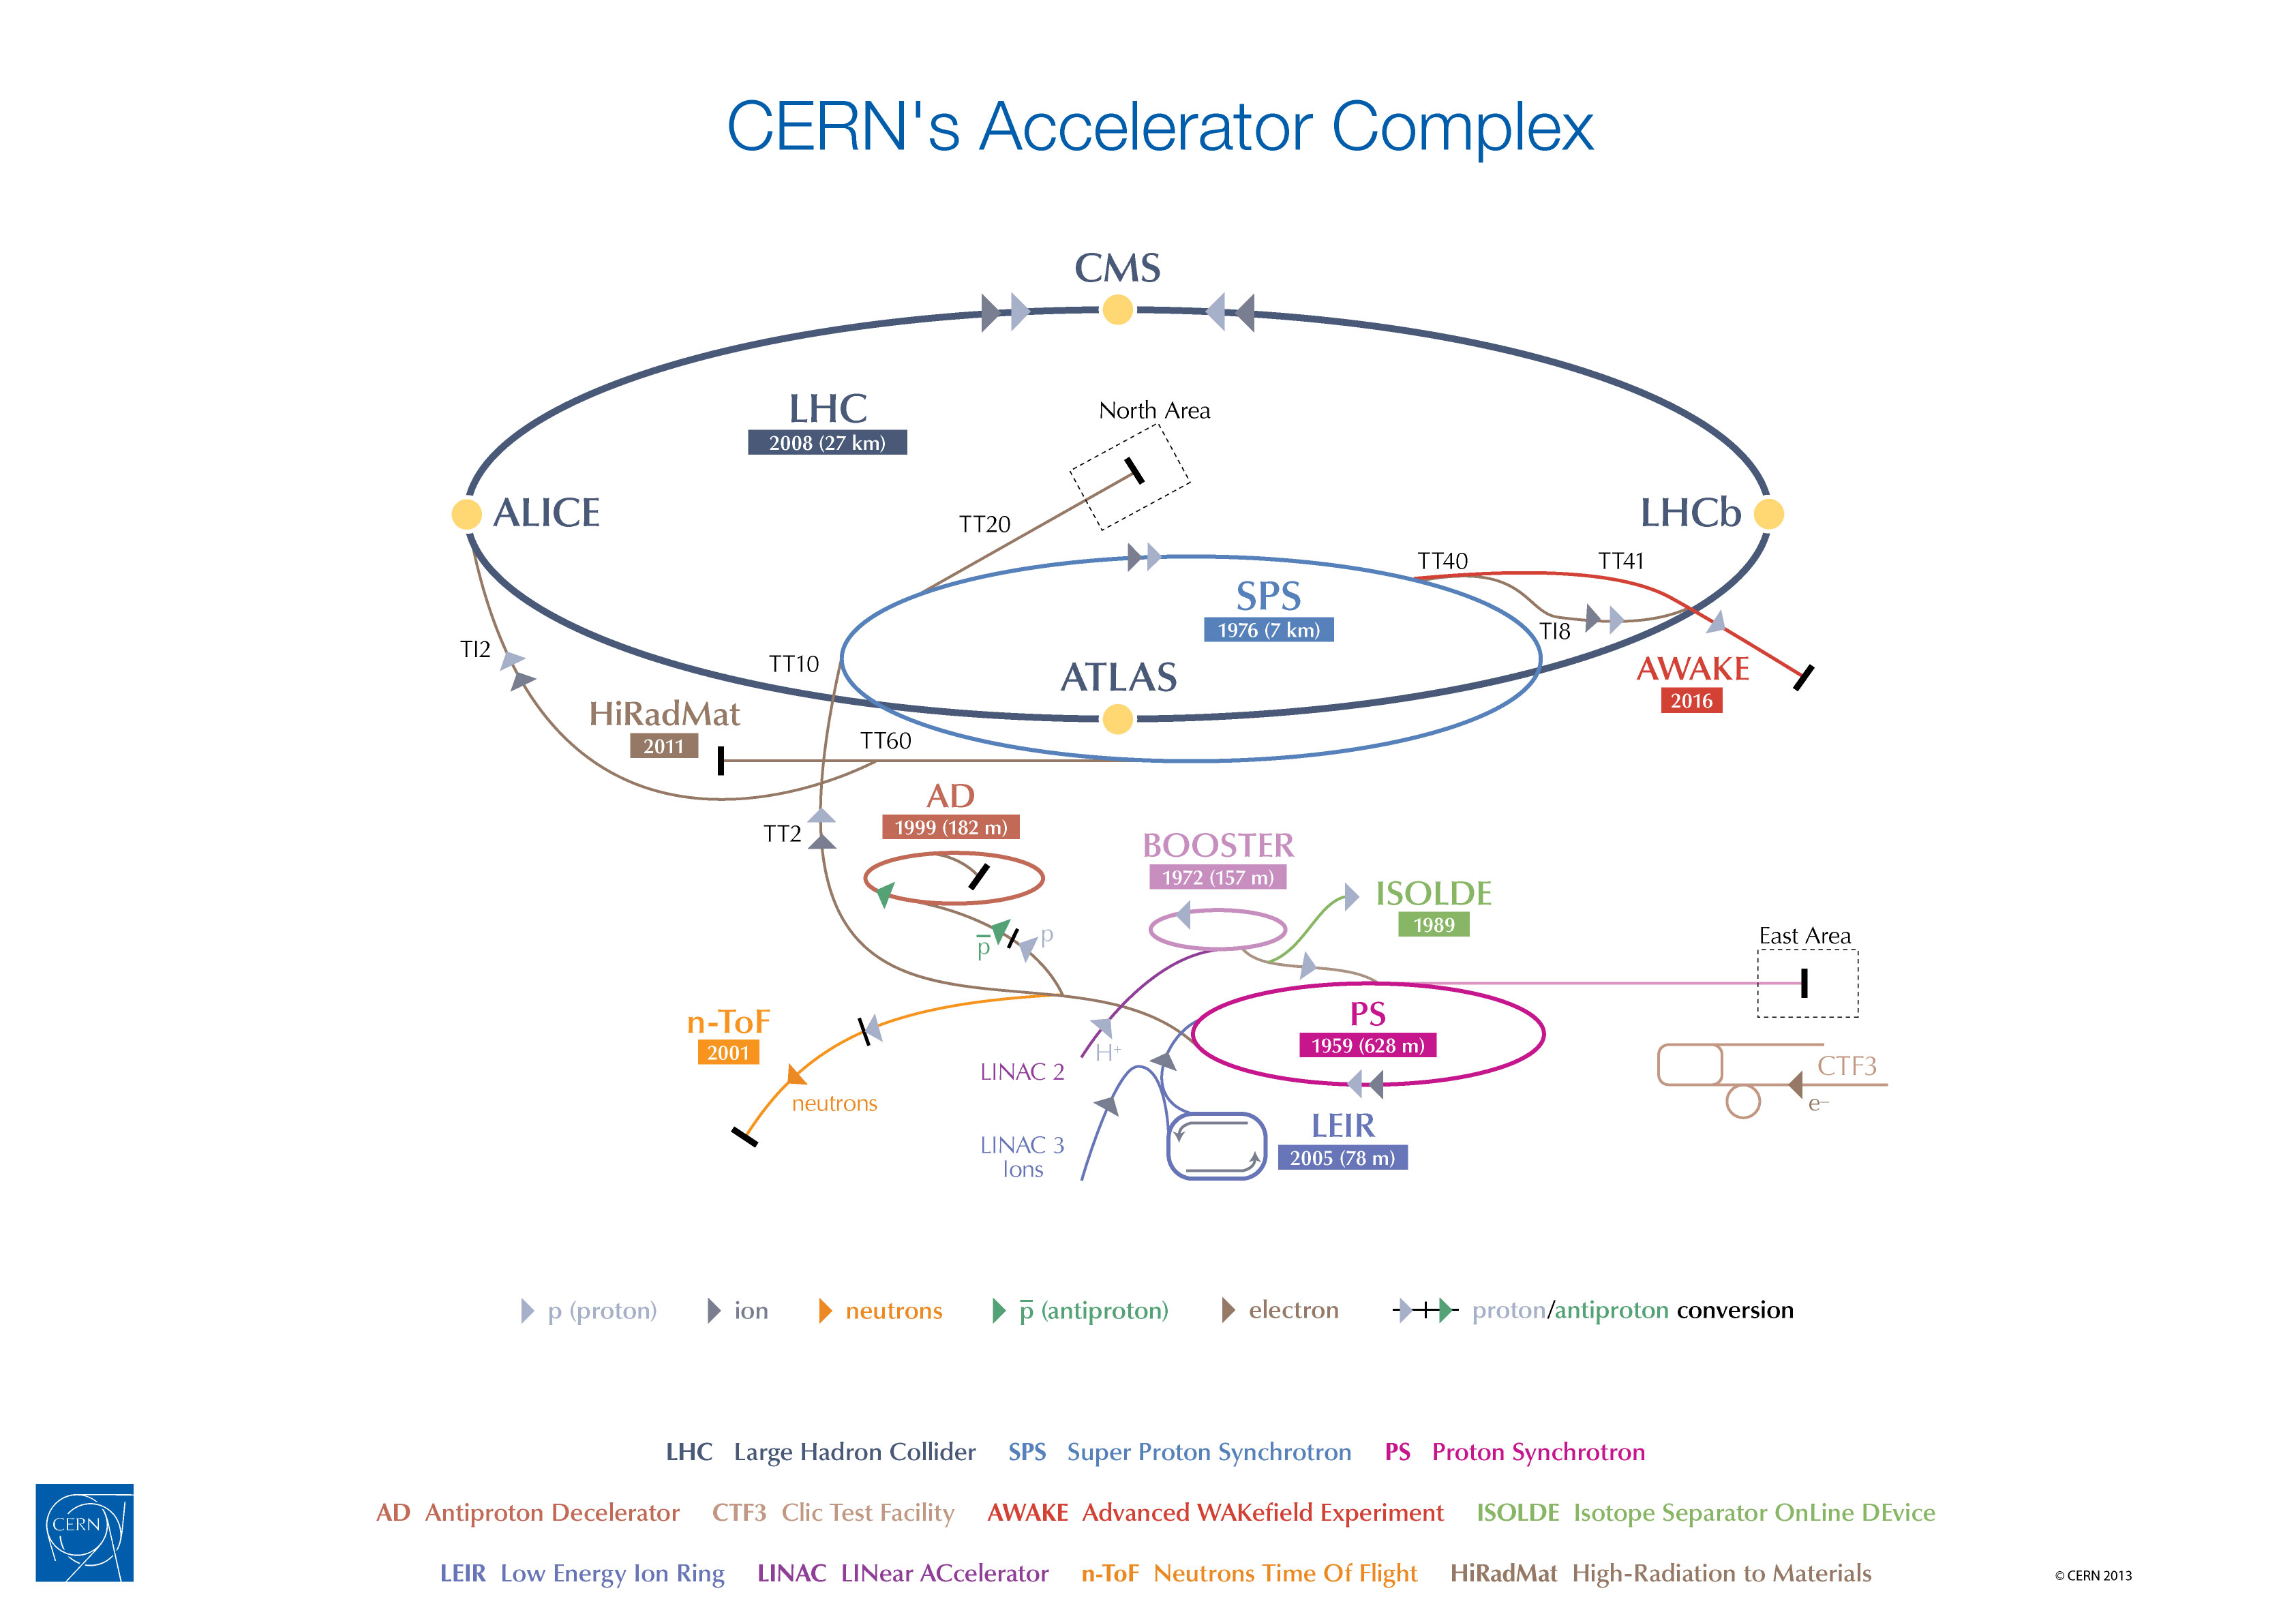
\includegraphics[width=\textwidth]{figures/Detector/CERNaccelerator}
\captionsetup{width=0.85\textwidth} \caption{\small Schematic view of the CERN accelerator complex. The four main LHC experiments are shown at the interaction points.}
\label{sec:det:fig:acccomplex}
\efig

Protons are obtained from hydrogen gas by breaking the molecules and stripping the electrons from hydrogen atoms. Protons are accelerated in the Linear Accelerator 2 (LINAC2) to 50 MeV and grouped into bunches. They are then transferred to the 157 m long Proton Synchrotron Booster (PSB), where they reach an energy of 1.4 $\gev$. After the PSB, protons are injected into the 628 m long Proton Synchrotron (PS), where their energy is ramped up to 25 $\gev$. In both the PSB and the PS protons are squeezed in very tight bunches that are the base bunch structure of the LHC. The last stage of preacceleration is done in the 7 km long Super Proton Synchrotron (SPS), where the protons are brought to an energy of 450 $\gev$ before injection into the LHC ring in two opposite directions. The connection between the LHC and the SPS is done through two 2.5 km long transfer lines.

\subsection{LHC design and machine parameters}
\label{chp:det:LHC:design}

One of the main contraints to reduce the cost of the LHC construction was the need to reuse the tunnel previously hosting the Large Electron Positron Collider (LEP).  The technological challenge of the LHC was the mass production of magnets necessary to maintain 7 $\tev$ protons in a circular trajectory with a radius of 4.3 km. A total of 1232 dipole magnets have been assembled in the LHC. Each magnet produces a bending field of up to 8.33 T thanks to superconducting coils made of niobium-titanium (NbTi) kept at a temperature of 1.9 K by superfluid helium. This makes the LHC the largest cryogenic system in the world. Each dipole contains two vacuum chambers in one single cryostat with magnetic fluxes that go in opposite directions, which allows the acceleration of two proton beams in opposite directions. This structure was needed to reduce the size of the cryostat and the cost of the cryogenic system.  The main acceleration from 450 $\gev$ to a maximum of 7 $\tev$  happens in the LHC with eight resonant Radio-Frequency (RF) cavities per beam. The electric field of those RF cavities oscillates at 400 MHz and increases the beam energy by 0.5 $\mev$/ turn. The field intensity at the maximum energy is around 5.5 MV/m.\\ \indent One of the important aspects in the design of an accelerator is the overall interaction rate that the LHC, in our case, can provide to the experiments.
The cross section, $\sigma$, describes the likelihood for a certain reaction -- the effective area that one particle presents to another particle for that reaction to occur. The instantaneous luminosity, $\lag(t)$, describes how frequently particles encounter each other, per unit of area and time. The overall interaction rate is equal to  $\sigma \times \lag(t)$. The total number of interactions for a certain process in a time interval [$t_{1}$,$t_{2}$], is given by:

\be
N_{\rm proc} = \int_{t_{1}}^{t_{2}} \sigma_{\rm proc} \times \lag(t) dt = \sigma_{\rm proc} \times \lag_{\rm int}(t_{1}, t_{2}),
\label{sec:det:eq:Nint}
\ee

\noindent where it is assumed that the cross section $\sigma_{\rm proc}$ does not depend on time and where $\lag_{\rm int}(t_{1}, t_{2})$ is the integrated luminosity for the time interval [$t_{1}$,$t_{2}$]. The requirement of high statistical accuracy of the data is translated into a requirement of high integrated luminosity of the accelerator. The instantaneous luminosity of the LHC at any Interaction Point (IP) depends on the beam bunch structure, the beam parameters and how well they can be controlled. For beams with equal parameters and approximately Gaussian spatial distributions, the instantaneous luminosity can be expressed as:

\be
\lag = N_{b} \cdot F\frac{n^{2}f_{\rm rev}}{4\pi \sigma_{xy}}, \,\, \sigma_{xy} = \sqrt{\frac{\epsilon\beta^{*}}{\gamma}},
\label{sec:det:eq:lumi}
\ee

\noindent where $N_{b}$ is the number of bunches present in each beam, $n$ is the number of protons in each bunch, $\sigma_{xy}$ is the transverse beam size at the IP, $f_{\rm rev}$ is the revolution frequencies of the bunches, $\gamma$ is the Lorentz factor, $\beta^{*}$ is the betatron function at the collision point, $\epsilon$ the normalised beam emittance, and $F$ is a geometric luminosity reduction factor that takes into account the beam crossing angle at the IP. 
The LHC beam parameters have been optimised to maximise the instantaneous luminosity at each IP taking into account various performance limitations and machine boundary conditions.\par
Due to the high frequency of collisions and the high density of the bunches necessary to achieve high luminosity, there is a non-zero probability that several events, originating from different $pp$ collisions, may occur simultaneously. These events are referred to as ``pileup'' and are categorised as in-time or out-of-time pileup. In-time pileup events are caused by additional $pp$ interactions in the same bunch crossing. The out-of-time pileup occurs when traces from an event in a different bunch crossing are recorded. The mean number of interactions per bunch crossing $\langle\mu\rangle$, which is taken as measure of the pileup activity, is shown in figure \ref{sec:det:fig:pileup}. The instantaneous luminosity is not constant over time, slowly degrading due to the bunch collisions, multiple Coulomb scattering within each bunch, and the scattering of protons against residual gas atoms inside the beam pipe. Therefore, the integrated luminosity depends on the luminosity lifetime, defined as the time that the beams are left orbiting in the LHC, and the beam turn-around time, defined as the time that passes between the beams being dumped and the beams being stable and ready for collisions again. More details about the LHC performance can be found in reference \cite{Bruning:2004ej}.

\bfig[h!]
\centering
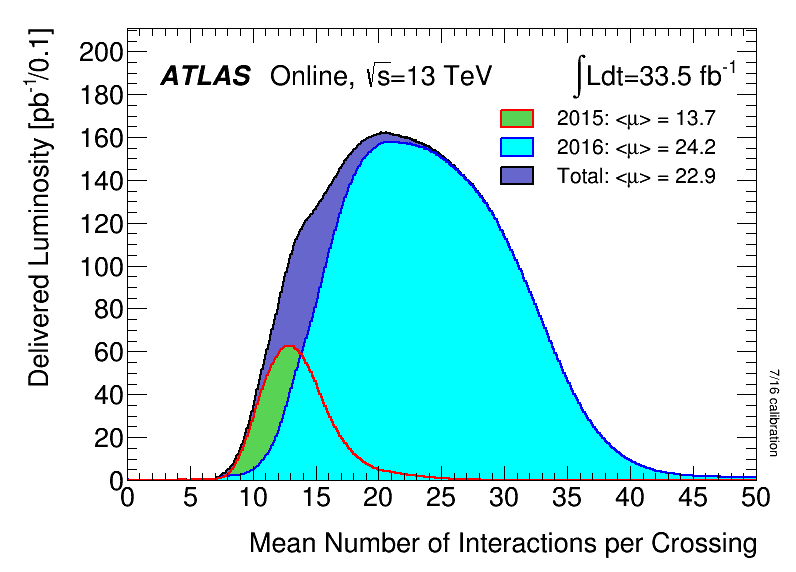
\includegraphics[width=0.5\textwidth]{figures/Detector/mu_2015_2016_LHCC.png}
\captionsetup{width=0.85\textwidth} \caption{\small Average number of interactions per beam crossing during the 2015 and 2016 LHC runs.}
\label{sec:det:fig:pileup}
\efig

\subsection{LHC experiments}

The LHC beams cross in four IPs, in each of which a particle detector is installed to record the collisions.  Earlier infrastructures, with some modifications to accommodate the LHC, were reused in order to further reduce the costs. Two of them are hosted in sites where before there were LEP experiments, while for the other two IPs new sites were needed. ATLAS \cite{ATLASjinst} and CMS \cite{CMS} are general-purpose experiments located at opposite IPs in the LHC ring. The independent design of the two experiments is of primary importance since it allows for cross-confirmation of measurements and possible new discoveries. LHCb \cite{LHCb} is a single-arm spectrometer designed to cover the forward region to perform dedicated studies of CP violation in $B$-meson decays and other studies of flavour physics, while ALICE \cite{ALICE} is designed to explore the formation of quark-gluon plasma in collisions of heavy ions. In addition to these four large experiments, three smaller experiments, LHCf \cite{LHCf}, TOTEM \cite{TOTEM} and MoEDAL \cite{MoEDAL}, are placed in the LHC ring. The LHCf experiment has been designed to study neutral hadrons emitted at low angles with respect to the beam pipe and it has been installed in the vicinity of ATLAS. CMS hosts TOTEM, which measures the total cross section through elastic and diffractive scattering of protons. The MoEDAL experiment is placed near LHCb and its purpose is the search for massive long-lived particles and magnetic monopoles.

\subsection{From first beam to world's record energy and luminosity}

After almost 15 years of prototyping the required technologies and an additional eight years of installation and commissioning of collider components, the LHC was officially completed and ready to start on the 10th of September 2008. Unfortunately, a serious accident occurred on the 19th of September, and the LHC operation had to be postponed and rescheduled. A faulty electrical connection
between two magnets ceased to be superconducting, causing mechanical failure of the cryogenic vessel followed by the leakage of around six tonnes of liquid helium. A total of 53 magnets were damaged and vacuum conditions in the beam pipe were lost. A total of 20 dipoles were replaced with spares, and new techniques to prevent a similar incident were developed. In December 2009 the LHC delivered first beams at a new world's record energy of 1.18 $\tev$. The new plan established that the LHC should provide proton beams of 3.5 $\tev$ during its initial operation from 2010 until 2012, and that it would be prepared to operate with proton beams of 7 $\tev$ only after a long shut-down period in 2013 and 2014.\par
In March 2010, Run 1 of the LHC started with the first collisions at a beam energy of 3.5 $\tev$, setting a new record for the energy achieved at a particle collider. The centre-of-mass energy was kept at 7 $\tev$ also during all of 2011. For the 2012 data taking the beam energy was increased to 4 $\tev$, for a center-of-mass energy of 8 $\tev$. In early 2010 the peak luminosity reached $2\times10^{32}$ cm$^{-2}$s$^{-1}$ obtained with $348$ colliding bunches of approximately $0.9 \times10^{11}$ protons each with a bunch spacing of 150 ns. In 2011 the peak luminosity reached $3.7\times 10^{33}$ cm$^{-2}$s$^{-1}$, increasing the number of bunches to 1380 with a minimum separation of 50 ns and the number of protons per bunch to $1.45 \times 10^{11}$. A further increase in luminosity was achieved by reducing the beam transverse size at the IP in order to increase the probability of $pp$ collisions per crossing. In 2012  a further reduction of the beam transverse size and an increase to the bunch intensity to 1.3 times the designed value allowed to reach a peak luminosity of $7.7\times10^{33}$ cm$^{-2}$s$^{-1}$. During the long shutdown (LS1), started on the 16th of February 2013, all electrical connections between superconducting magnets were consolidated allowing the LHC to reach higher energy and luminosity during Run 2. In figure \ref{sec:det:fig:consolidations} a summary of the LHC maintenance carried out during LS1 is shown.\par
In June 2015 LHC Run 2 started recording the first collisions at a beam energy of 6.5 $\tev$, setting a new record. During the year the number of bunches was increased up to 2244 with a minimum separation of 25 ns. For 2016 data taking the LHC achieved the current luminosity record for a hadron machine of $1.4 \times 10^{34}$ cm$^{-2}$s$^{-1}$  by further reducing the beam transverse size. Table \ref{sec:det:tab:LHCparam} shows the values of the beam parameters for the design operation, as well as those used during Run 1 and early Run 2 data taking.

\bfig[t!]
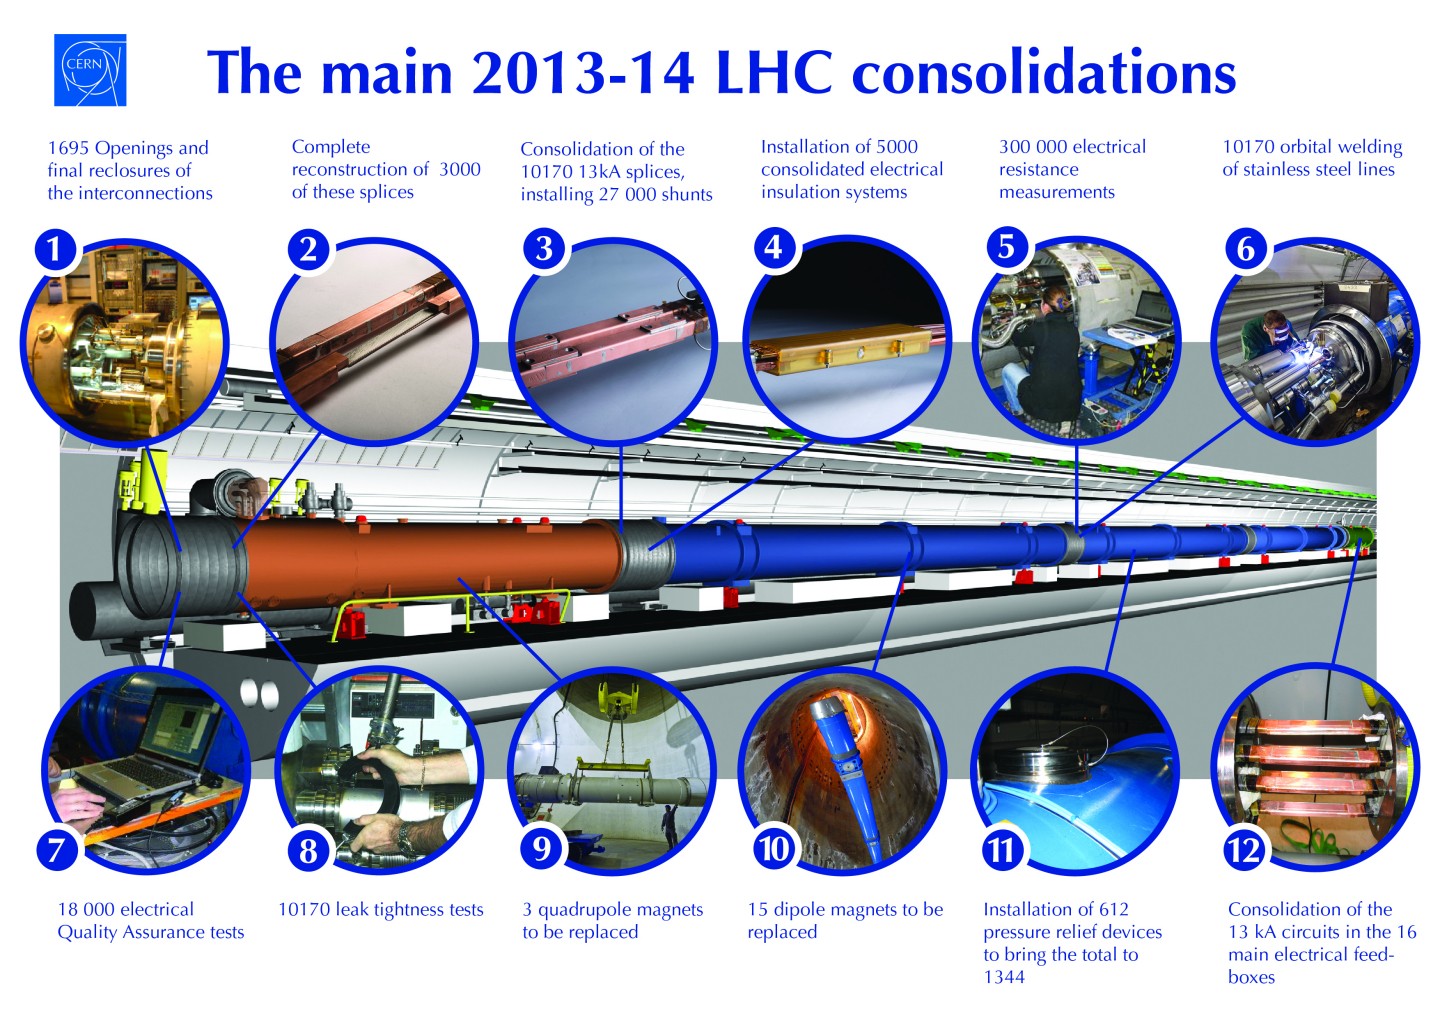
\includegraphics[width=\textwidth]{figures/Detector/LHCconsolidationsEng.jpg}
\captionsetup{width=0.85\textwidth} \caption{\small The main LHC consolidations during LS1.}
\label{sec:det:fig:consolidations}
\efig


\begin{table}
\footnotesize
\begin{center}
\begin{tabular}{c|c|c|c|c}
  \hline \hline
  Parameter & Design value & Run 1 & 2015 & 2016 \\
  \hline
  Beam energy ($\tev$) & 7 & 3.5--4 & 6.5 & 6.5 \\
  Beta function $\beta^{*}$ (m) & 0.55 & 1.5--0.6 & 0.8 & 0.4 \\
  Maximum num. bunches/beam & 2808 & 1380 & 2244 & 2220 \\
  Max. num. protons/bunch & $1.15\times10^{11}$ & $(1.45--1.7)\times10^{11}$ & $1.15\times10^{11}$ & $1.3\times10^{11}$\\ 
  Bunch spacing (ns) & 25 & 75--50 & 50--25 & 25 \\
  Peak luminosity (cm$^{-2}$s$^{-1}$ ) & $1\times10^{34}$  & $7.7\times10^{33}$  & $6\times10^{33}$  & $1.4\times10^{34}$  \\
  Emittance $\epsilon_{n} (\mu {\rm rad})$ & 3.75 & 2.5 & 2.5& 2.5 \\
 Max. $\langle\mu\rangle$ & 19 & 37 & 30 & 50 \\
  \hline\hline

\end{tabular}
\captionsetup{width=0.85\textwidth} \caption{\small Overview of the LHC beam parameters comparing the design values with their time evolution during Run 1 and early Run 2 operations.}
\label{sec:det:tab:LHCparam}
\end{center}
\end{table}


\section{The ATLAS experiment}
\label{chp:det:ATLAS}

ATLAS (A Toroidal LHC ApparatuS) \cite{ATLASjinst}, is a multi purpose detector designed to measure particles produced in $pp$ collisions at unprecedented energies and instantaneous luminosities. The guidelines in the detector construction and specifications were driven by the goals of maximising the discovery potential for new phenomena while keeping the ability to perform precise measurements of known processes \cite{ATLASTDR1}. Among the priorities of the experiment was the search for the Higgs boson (and the measurement of its properties) as well as the search for new exotic (e.g. supersymmetric) particles that might be part of possible extensions of the SM. Furthermore the luminosity delivered by the LHC allows to collect a very large sample of vector bosons ($W$ and $Z$), $B$-mesons and top quarks, which gives the possibility to perform detailed studies on QCD, CP violation and top quark properties. At the same time, the possibility to observe unexpected phenomena demanded a very flexible design, not excessively tied to a specific physics model. For this reason, the detector is required to identify and measure the kinematic properties of a large spectrum of particles that are produced in $pp$ collisions over a wide energy range (from few $\gev$ to $\tev$). This includes charged leptons (electrons, muons, taus), photons, jets produced by the hadronisation of quarks and gluons, as well as particles that escape ``direct'' detection like neutrinos and other new weakly-interacting particles. These latter are identified through the measurement of transverse-momentum imbalance in the event, the missing transverse energy (\MET).\par
A schema of the ATLAS detector is shown in figure \ref{sec:det:fig:ATLAScoordinates} . It measures 44 m in length and 25 m in diameter for a total weight of 7000 tons. Like most collider detectors, ATLAS has a cylindric geometry to cover the full solid angle around the interaction point with the various subdetectors arranged in concentric layers. Starting from the centre, the Inner Detector (ID) is designed to reconstruct the trajectories of charged particles (tracks) and measure their momenta from the radius of curvature in a solenoidal magnetic field. The Inner Detector is surrounded by an electromagnetic and a hadronic calorimeter that measure the energies of electrons/photons and hadrons by detecting the showers produced by the particles' interactions with their absorber materials. Muons are the only directly-detectable particles that pass through the thick calorimeter. They are detected with a spectrometer embedded in a toroidal magnetic field.\\ The following specifications have been taken into account in the construction of the detector:
\bi
\ib efficient track reconstruction and good track momentum resolution;
\ib precise measurement of track quantities and secondary vertices for the identification of jets produced by $b$-/$c$-quarks and $\tau$-leptons;
\ib an electromagnetic calorimeter with excellent angular and energy resolution for the measurements of electrons and photons;
\ib a hermetic hadronic calorimeter with large angular coverage for the measurement of jets and missing transverse energy;
\ib good muon identification and momentum reconstruction up to highest luminosity with the possibility to determine the charge of high-\pT muons;
\ib large acceptance in pseudorapidity ($\eta$) with almost full azimuthal angle ($\phi$) coverage;
\ib a flexible trigger system capable of maintaining high selection efficiency and sufficient background rejection even for low-/medium-\pT objects.
\ei

In addition to these requirements, specific conditions from the LHC operation pose additional constraints on the detector design. Due to the high interaction rate of 40 MHz, fast electronics is employed in the readout of all sub detectors, while the large
number of interactions per crossing and the consequent large particle flux requires sensors resistant to high-radiation doses. At the same time, highly-granular detectors are required to reduce the impact of overlapping interactions.

\bfig[t!]
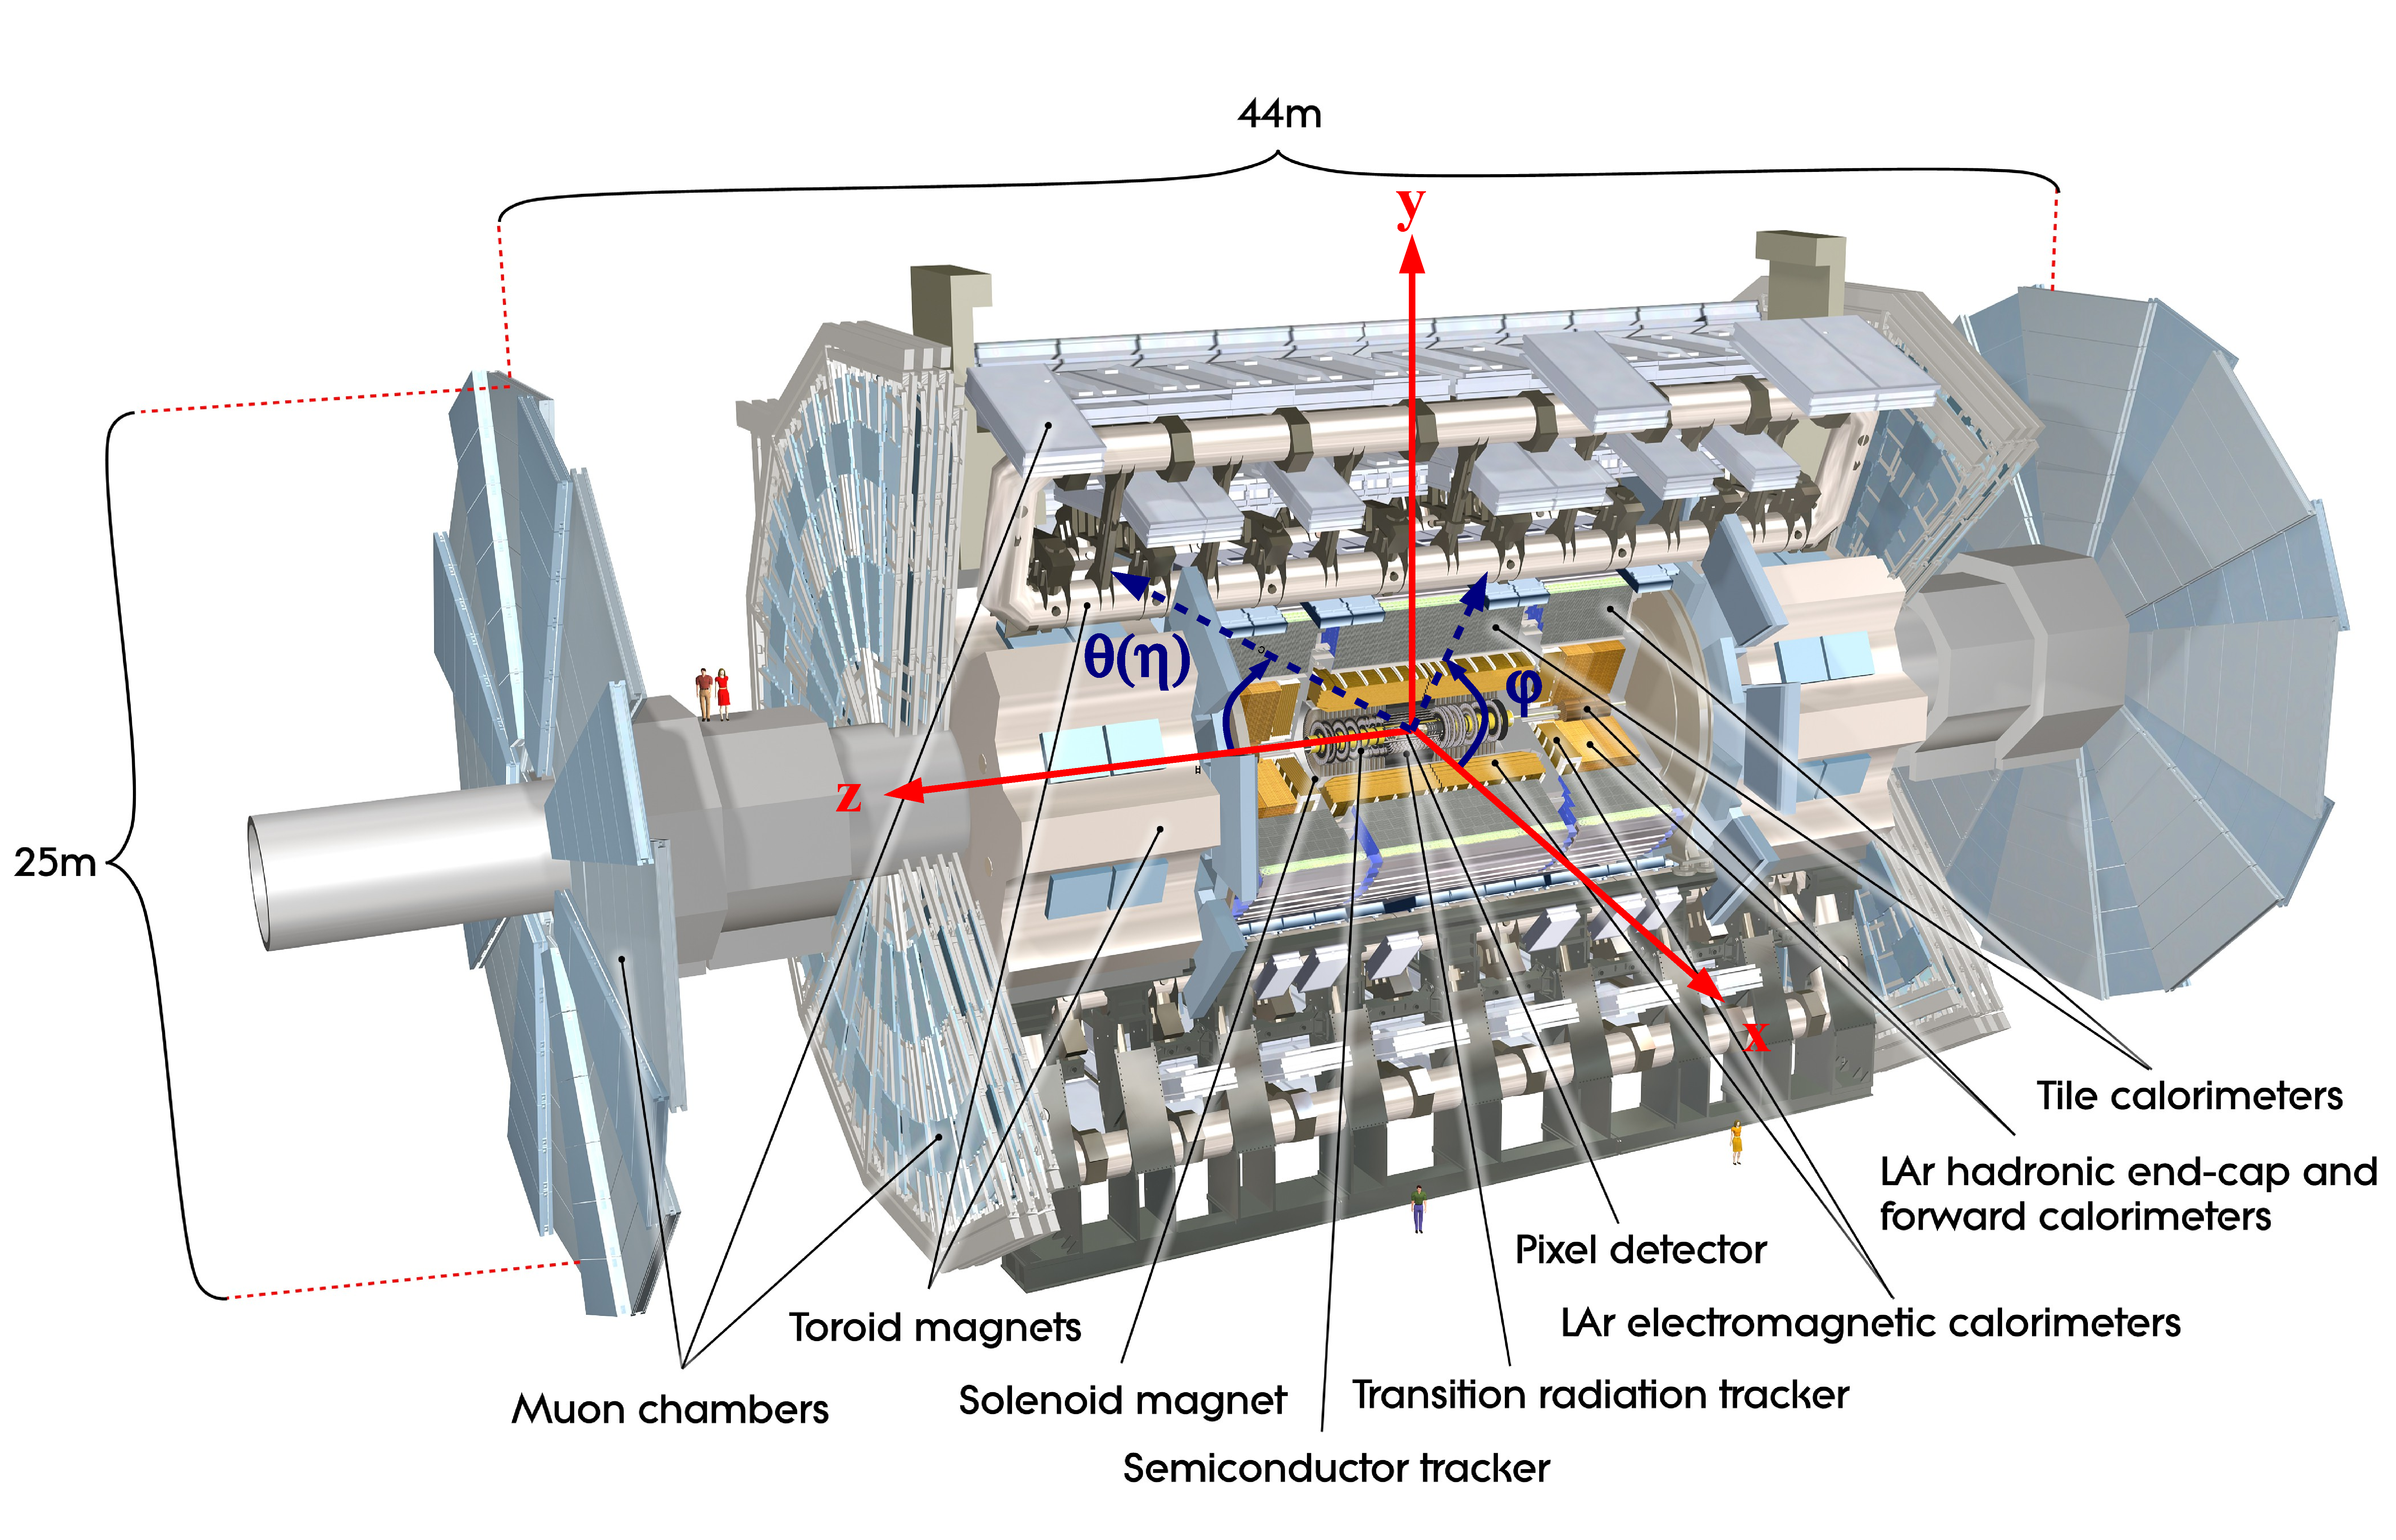
\includegraphics[width=1.1\textwidth]{figures/Detector/atlas_coordinates.png}
\captionsetup{width=0.85\textwidth} \caption{\small View of the ATLAS detector along with the coordinate system.}
\label{sec:det:fig:ATLAScoordinates}
\efig

\subsection{Coordinate system}
The ATLAS coordinate system is right-handed in which $x$-axis points to LHC's center, the $z$-axis follows the beam direction and the $y$-axis points upwards away from the centre of the Earth. The origin of the coordinate system is defined by the nominal interaction point of the beams. The region delimited by positive values of the $z$ coordinate, is referred to as ``A side'', while the region with negative values is referred to as ``C side''. At hadron colliders spherical coordinates are commonly used. The azimuthal angle $\phi$ is measured around the beam axis, ranging between $-\pi$ and $+\pi$ with respect to the $x$-axis. The polar angle $\theta$ is measured with respect to the $z$-axis and ranges between 0 and $\pi$. Since the momentum of the colliding partons along the $z$-axis is unknown, it is useful to define the transverse component of variables of interest, like energy and momentum, defined as the projection on the $xy$ plane, which are boost-invariant along the $z$-axis:
\be
\pt = \sqrt{p_{x}^{2}+p_{y}^{2}}=|\vec p|\sin\theta, \,  E_{T} = E\sin\theta.
\label{sec:det:eq:ptdefinition}
\ee

\noindent Another angular quantity, used at hadron colliders to describe the polar distribution and preferred\footnote{The advantage over $\theta$ is that rapidity differences $\Delta y$ are boost-invariant along the $z$-axis.} to the simple polar angle $\theta$ is the rapidity $y$:

\be
y = \frac{1}{2}\ln\left(\frac{E+p_{\rm z}}{E-p_{\rm z}}\right),
\label{sec:det:eq:rapidity}
\ee

\noindent which, for vanishing particle mass, is equal to the pseudorapidity $\eta$:

\be
\eta = -\ln\left(\tan\frac{\theta}{2}\right).
\label{sec:det:eq:pseudorapidity}
\ee

\noindent The angular separation in the $\eta$-$\phi$ plane between particles is defined as:

\be
\Delta R = \sqrt{(\Delta \eta)^{2}+(\Delta \phi)^{2}}.
\label{sec:det:eq:deltaRdefinition}
\ee



\subsection{Magnet system}
The magnet system \cite{ATLASTDR1} represents a particular characteristic of the ATLAS experiment that has a peculiar design compared to other high-energy physics experiments. It is composed of four large superconducting magnets, cooled with liquid helium at 4.5 K, designed to provide a field mostly orthogonal to the particle trajectory. It consists of a central solenoid and three open-air toroids, as shown in figure \ref{sec:det:fig:ATLASmagnets}. This hybrid solution has the advantage of extending the pseudorapidity coverage ($|\eta|<3$), and having no magnetic field inside the calorimeters in order not to degrade their performances. Furthermore, the open-air design for the toroids reduces the impact of multiple scattering on the momentum resolution and improves the muon reconstruction without relying on the Inner Detector.\par
\bfig[htb!]
\centering
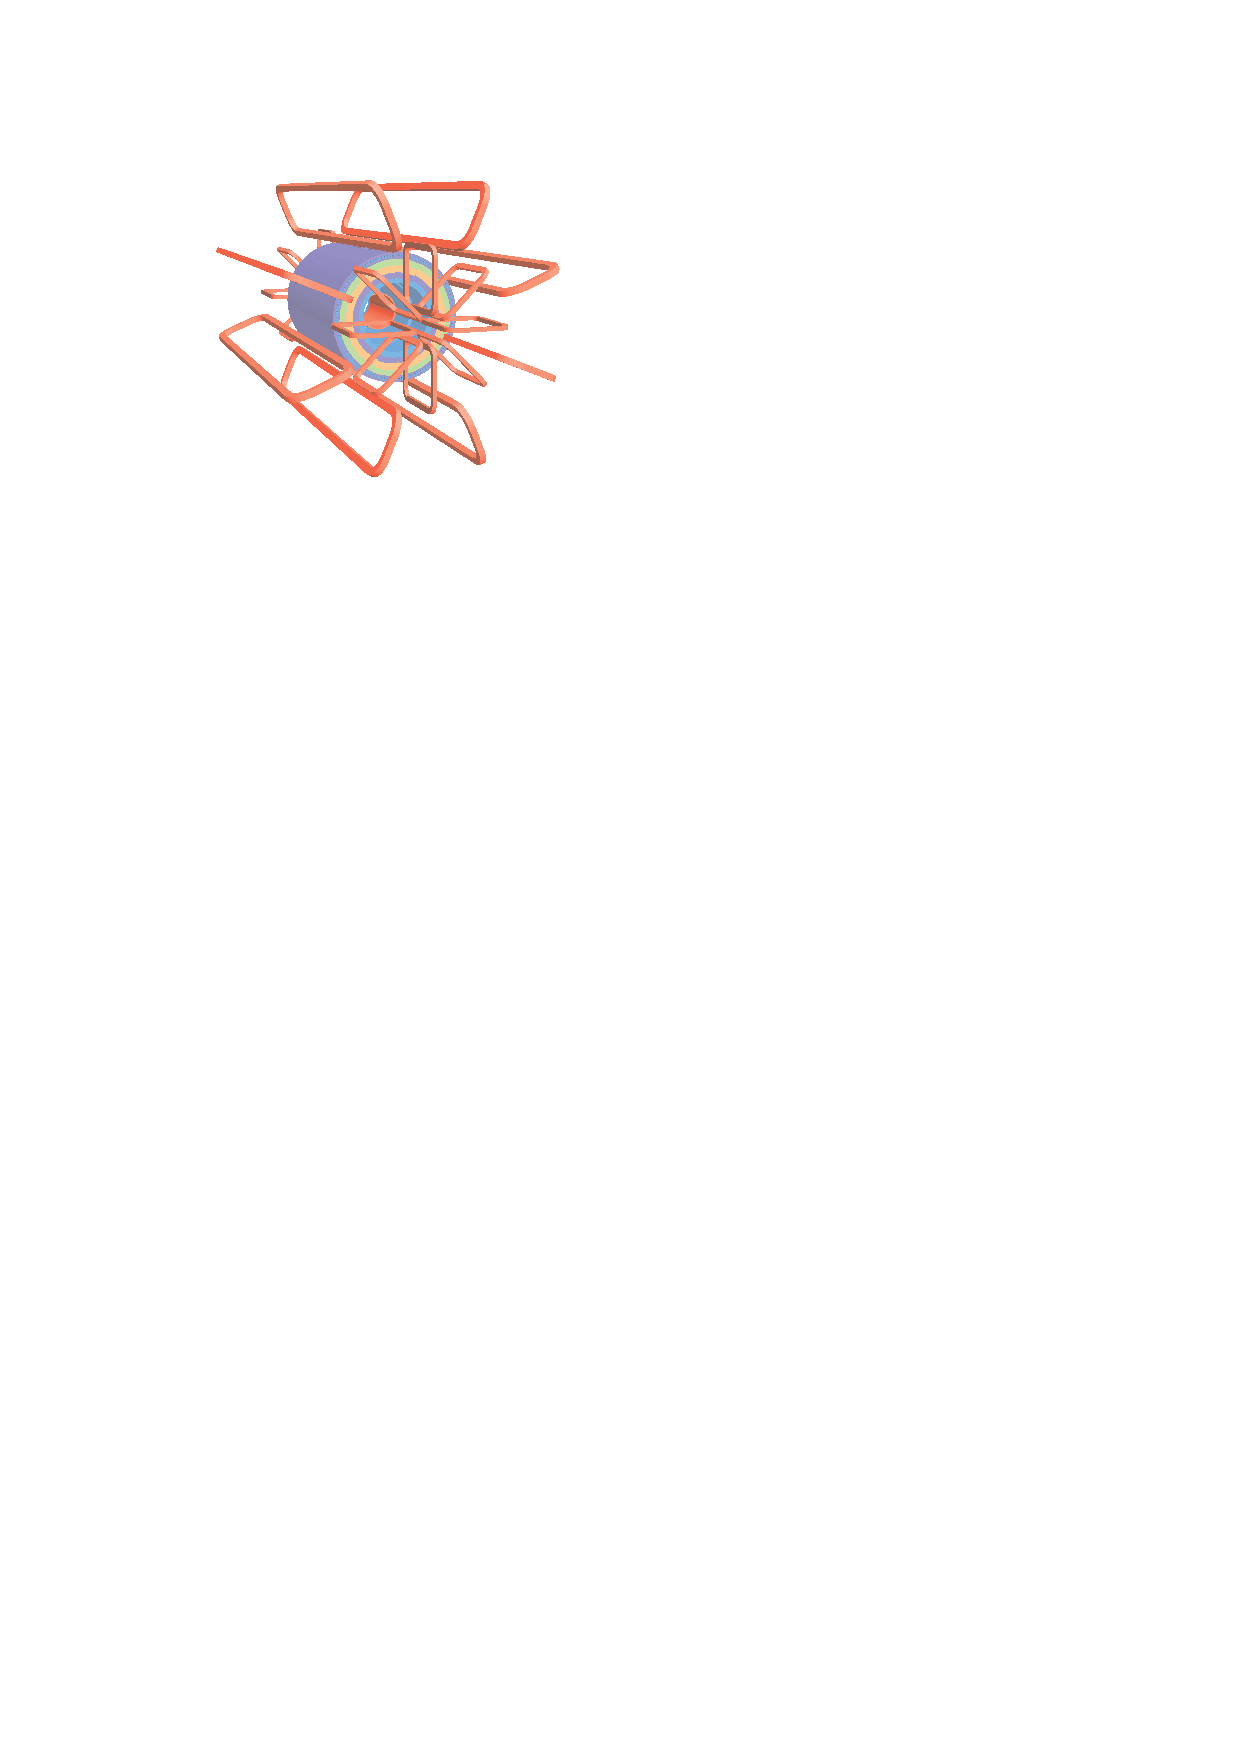
\includegraphics[width=0.5\textwidth]{figures/Detector/magnets.png}
\captionsetup{width=0.85\textwidth} \caption{\small The ATLAS magnet system. The eight coils of the barrel and end-cap toroids are visible. The solenoid is inside the calorimeter and it is shown as four layers with different magnetic properties.}
\label{sec:det:fig:ATLASmagnets}
\efig
The central solenoid (CS) provides a magnetic field to the Inner Detector parallel to the beam axis bending particles in the $\phi$ direction. The CS is 5.3 m long and it has a radius of 2.5 m.  The coil of the CS was designed to be the thinnest possible to limit the amount of material in front of the calorimeters, but still thick enough to ensure safety and reliability during operation. Also to minimise the amount of material in front of the calorimeter, one cooling cryostat is shared between the CS and the Liquid Argon Calorimeter. The magnetic field is 2 T with a peak of 2.6 T on the superconductor. As the distance from the interaction point increases in the $z$ direction, the field strength decreases as result of the finite size of the solenoid.\par
The toroidal system generates the field necessary to bend particles in the muon spectrometer. The system is composed by two End-Cap Toroids (ECT) at the extremities of the detector and a Barrel Toroid (BT) centrally located around the calorimeters. The ECT are 5 m long and have an external diameter of 10.7 m, while the BT is 26 m long with a diameter of 20 m. Each toroid is composed of eight rectangular coils arranged in the radial direction from the beam axis. The ECT are rotated by $22.5^{\circ}$ with respect to the BT in order to generate a radial overlap for a higher magnetic field uniformity and to optimise the bending power in the transition regions. Each coil of the BT has its own cryostat, while for the end-cap toroids all the coils are in the same cryostat that is shared with the forward calorimeter. The magnetic fields generated by the BT and ECT are 3.9 T and 4.1 T respectively. 


\subsection{Inner detector}

The ATLAS Inner Detector (ID) \cite{ATLASTDR1} is designed to provide efficient pattern recognition and good momentum resolution for charged particles in the range $|\eta|<2.5$ from $\pt$ as low as 0.4 $\gev$ up to a few $\tev$. At the same time, its capability of precisely reconstructing primary and secondary vertices and measuring the track parameters is of primary importance for identifying the decays of short-lived particles. A precise measurement of the particle curvature in the solenoidal magnetic field requires a good spatial resolution. In presence of a high density of particles emerging from the interaction point, this can be achieved only with high granularity. The chosen configuration results from a compromise between high performance, economical budget and amount of material used in the tracker. A large amount of material can in fact degrade the intrinsic momentum resolution due to multiple scattering, as well as the performance of the calorimeter. The overall thickness of the ID is about 0.4 radiation lengths ($X_{0}$) and increases up to 1.5 $X_{0}$ in the forward region due to the presence of services (e.g. cables for the electronic boards and the cooling system). The structure of the ID is shown is figure \ref{sec:det:fig:ATLASID}.
 \bfig[tb!]
\centering
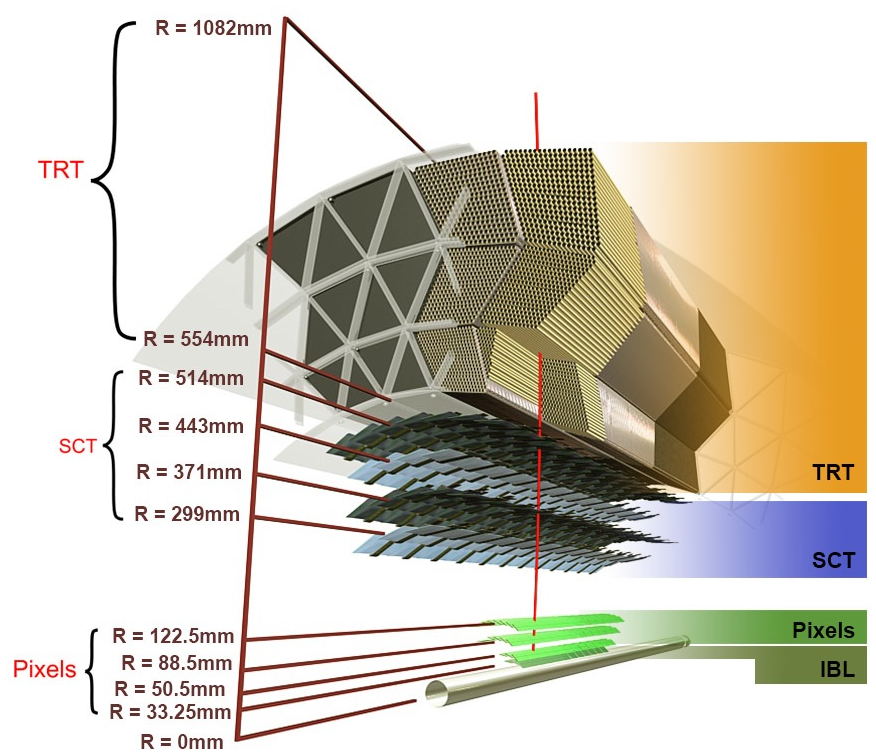
\includegraphics[width=0.7\textwidth]{figures/Detector/fig_01.png}
\captionsetup{width=0.85\textwidth} \caption{\small Representation of the structure of the Inner Detector and its three subdetectors.}
\label{sec:det:fig:ATLASID}
\efig
It combines three different technologies reflecting the different track densities that can be found when increasing the distance from the interaction point. High-resolution detectors are located in the innermost region using semiconductor technology. At larger distance from the interaction point, a detector with lower intrinsic resolution, a transition radiation detector based on drift tubes, allows to collect a larger number of measurements working in a continuous tracking mode.
The three components are:
\bi
\ib Pixel Detector,
\ib SemiConductor Tracker (SCT), and
\ib Transition Radiation Tracker (TRT).
\ei
 
In the barrel the layers of each subdetector are composed of concentric cylinders oriented in the direction of the beam axis while in the forward region are composed of disks/wheels arranged orthogonally to the beam direction. The ID is 7 m long and it has an external radius of 1.15 m, fully contained in the CS. The relative precision of the three subdetectors is comparable so that no single measurements dominates the momentum resolution. This redundancy also guarantees high efficiency even in case a part of one of the subdetectors is malfunctioning. Combining the information from the three subdetectors, the ID reaches a designed resolution of the track momentum of:

\be
\frac{\sigma_{\pt}}{\pt} = 0.05 \% \times \pt(\gev) \oplus 0.1 \%.
\label{sec:det:eq:IDresolution}
\ee



\subsubsection{Pixel detector}

The silicon pixel technology is the only solution that guarantees good pattern recognition performance in a very dense track environment such as the one close to the LHC interaction point. The ATLAS Pixel detector has been designed to provide at least four precise hits for the track reconstruction in the proximity of the interaction point;
 the precise reconstruction of the primary vertex makes use as well of those hits. The pixel detector with its design and location is also important for measurement of the track impact parameter, which is defined as the minimum distance of the track to the primary vertex. This is one of the main quantities used in the identification of $b$/$c$-hadrons and $\tau$-leptons. The resolution on the track impact parameter is completely dominated by the performance of the pixel detector.\par  The detector is organised in a barrel and two end-caps. The barrel is composed of four cylinders: the layer closest to the beam pipe is 62 cm long and has a radius of 3.325 cm (Insertable B-Layer or IBL) \cite{IBLTDR}, installed during the LS1, and the three outer cylinders are 80 cm long and have radii of 5.05 cm (B-Layer), 8.85 cm (Layer 1) and 12.25 cm (Layer 2). Each end-cap contains three disks with a radius of 34 cm placed at distances of $|z|$ = 49.5, 58.0 and 65.0 cm from the centre of the detector. To obtain high granularity the silicon chips are segmented in a matrix of pixels allowing simultaneous measurements of the two spatial coordinates. The dimensions of a single pixel are $50\times250$ $\mu $m$^{2}$ and $50\times400$ $\mu $m$^{2}$ respectively for the IBL and the other layers. The shortest dimension of the sensor is aligned in the direction of the bending plane of the particle in order to achieve the best performance. The average position resolution is equal to 10 $\mu$m in the direction of the short pixel pitch and 65 $\mu$m (115 $\mu$m) in the direction of the long pixel pitch for the IBL (three outer layers). The basic unit of the detector is the module, which contains the silicon sensor and the required electronics. The matrix in each module has $80\time336$ pixels and $144\times328$ pixels respectively in the IBL and the other layers. In total $\sim2500$ modules were assembled in the barrel and endcap for a total of 92 million channels. The pixel detector needs high thermal stability to keep good performance and a low temperature to minimise radiation damage. The IBL temperature during 2015 and 2016 was kept between $-15\,^{\circ}\mathrm{C}$ and $5\,^{\circ}\mathrm{C}$. The other layers are kept at temperature between $-10\,^{\circ}\mathrm{C}$ and $-15\,^{\circ}\mathrm{C}$.

\subsubsection{Semiconductor tracker}

The SCT has been designed to provide at least eight precise points per track. Thanks to its high granularity, it contributes to the track reconstruction and momentum measurement. The detector is organised in a barrel with four cylinders and two end-caps with nine disks. The cylinders have a structure in carbon fibre with radii of 30.0, 37.3, 44.7 and 52.0 cm, on which several longitudinal staves are mounted and equipped with the semiconductor modules. In the end-caps the disks have the modules arranged in the radial direction. The basic unit of the detector is the module and contains two single-sided silicon microstrip sensors mounted back-to-back. Each sensor has an active area of $6.36\times6.40$ cm$^{2}$ and contains 768 microstrips with 80 $\mu$m width. In the barrel the $R-\phi$ coordinate of the hit is determined by the strip position, while a precise measurement of the $z$ coordinate is obtained exploiting the stereoscopic effect: the back-to-back sensors are mounted with a 40 mrad ``tilt'' angle, so the crossing point of the strips on both sensors on each module is used to determine the space-point position. In the end-cap, the $\phi$ coordinate of the track is determined using the strip position and the $R$-coordinate with the ``stereo'' effect. The spatial resolution achieved is 17 $\mu$m in the direction of the strip pitch, and 580 $\mu$m in the direction determined by the strip crossing. For the same reasons as in the Pixel Detector, the SCT is kept at a temperature between $-5\,^{\circ}\mathrm{C}$ and $-15\,^{\circ}\mathrm{C}$.

\subsubsection{Transition radiation tracker}
The TRT, the outermost part of the three tracking subsystems of the ID, is a straw-tube tracker particularly well suited to LHC conditions due to its resistance to radiation. The barrel region contains 52544 straw tubes with a length of 1.5 m arranged parallel to the beam axis. Barrel tubes have the central wires electrically split and read out at both ends of the straw. Each end-cap contains 122880 straw tubes with a length of 0.4 m arranged perpendicularly to the beam axis, and read out at their outer end. Each drift tube has a diameter of 4 mm that is made from wound Kapton and carbon fibre; in the centre of each tube there is a gold-plated tungsten wire of 31 $\mu$m diameter and the tube is filled with a gas mixture. Most of the TRT is filled with a mixture of $70\,\%$ Xe, $27\,\%$ CO$_{2}$, and $3\,\%$ O$_{2}$. Due to large irreparable gas leaks that developed in the gas system, part of the TRT detector is now flushed with a gas mixture composed primarily of much cheaper argon, $80\,\%$ Ar and $20\,\%$ CO$_{2}$ (see figure \ref{sec:det:fig:trfgas}).

\begin{figure}[tb!]
  \begin{subfigure}{0.5\textwidth}
  \centering
  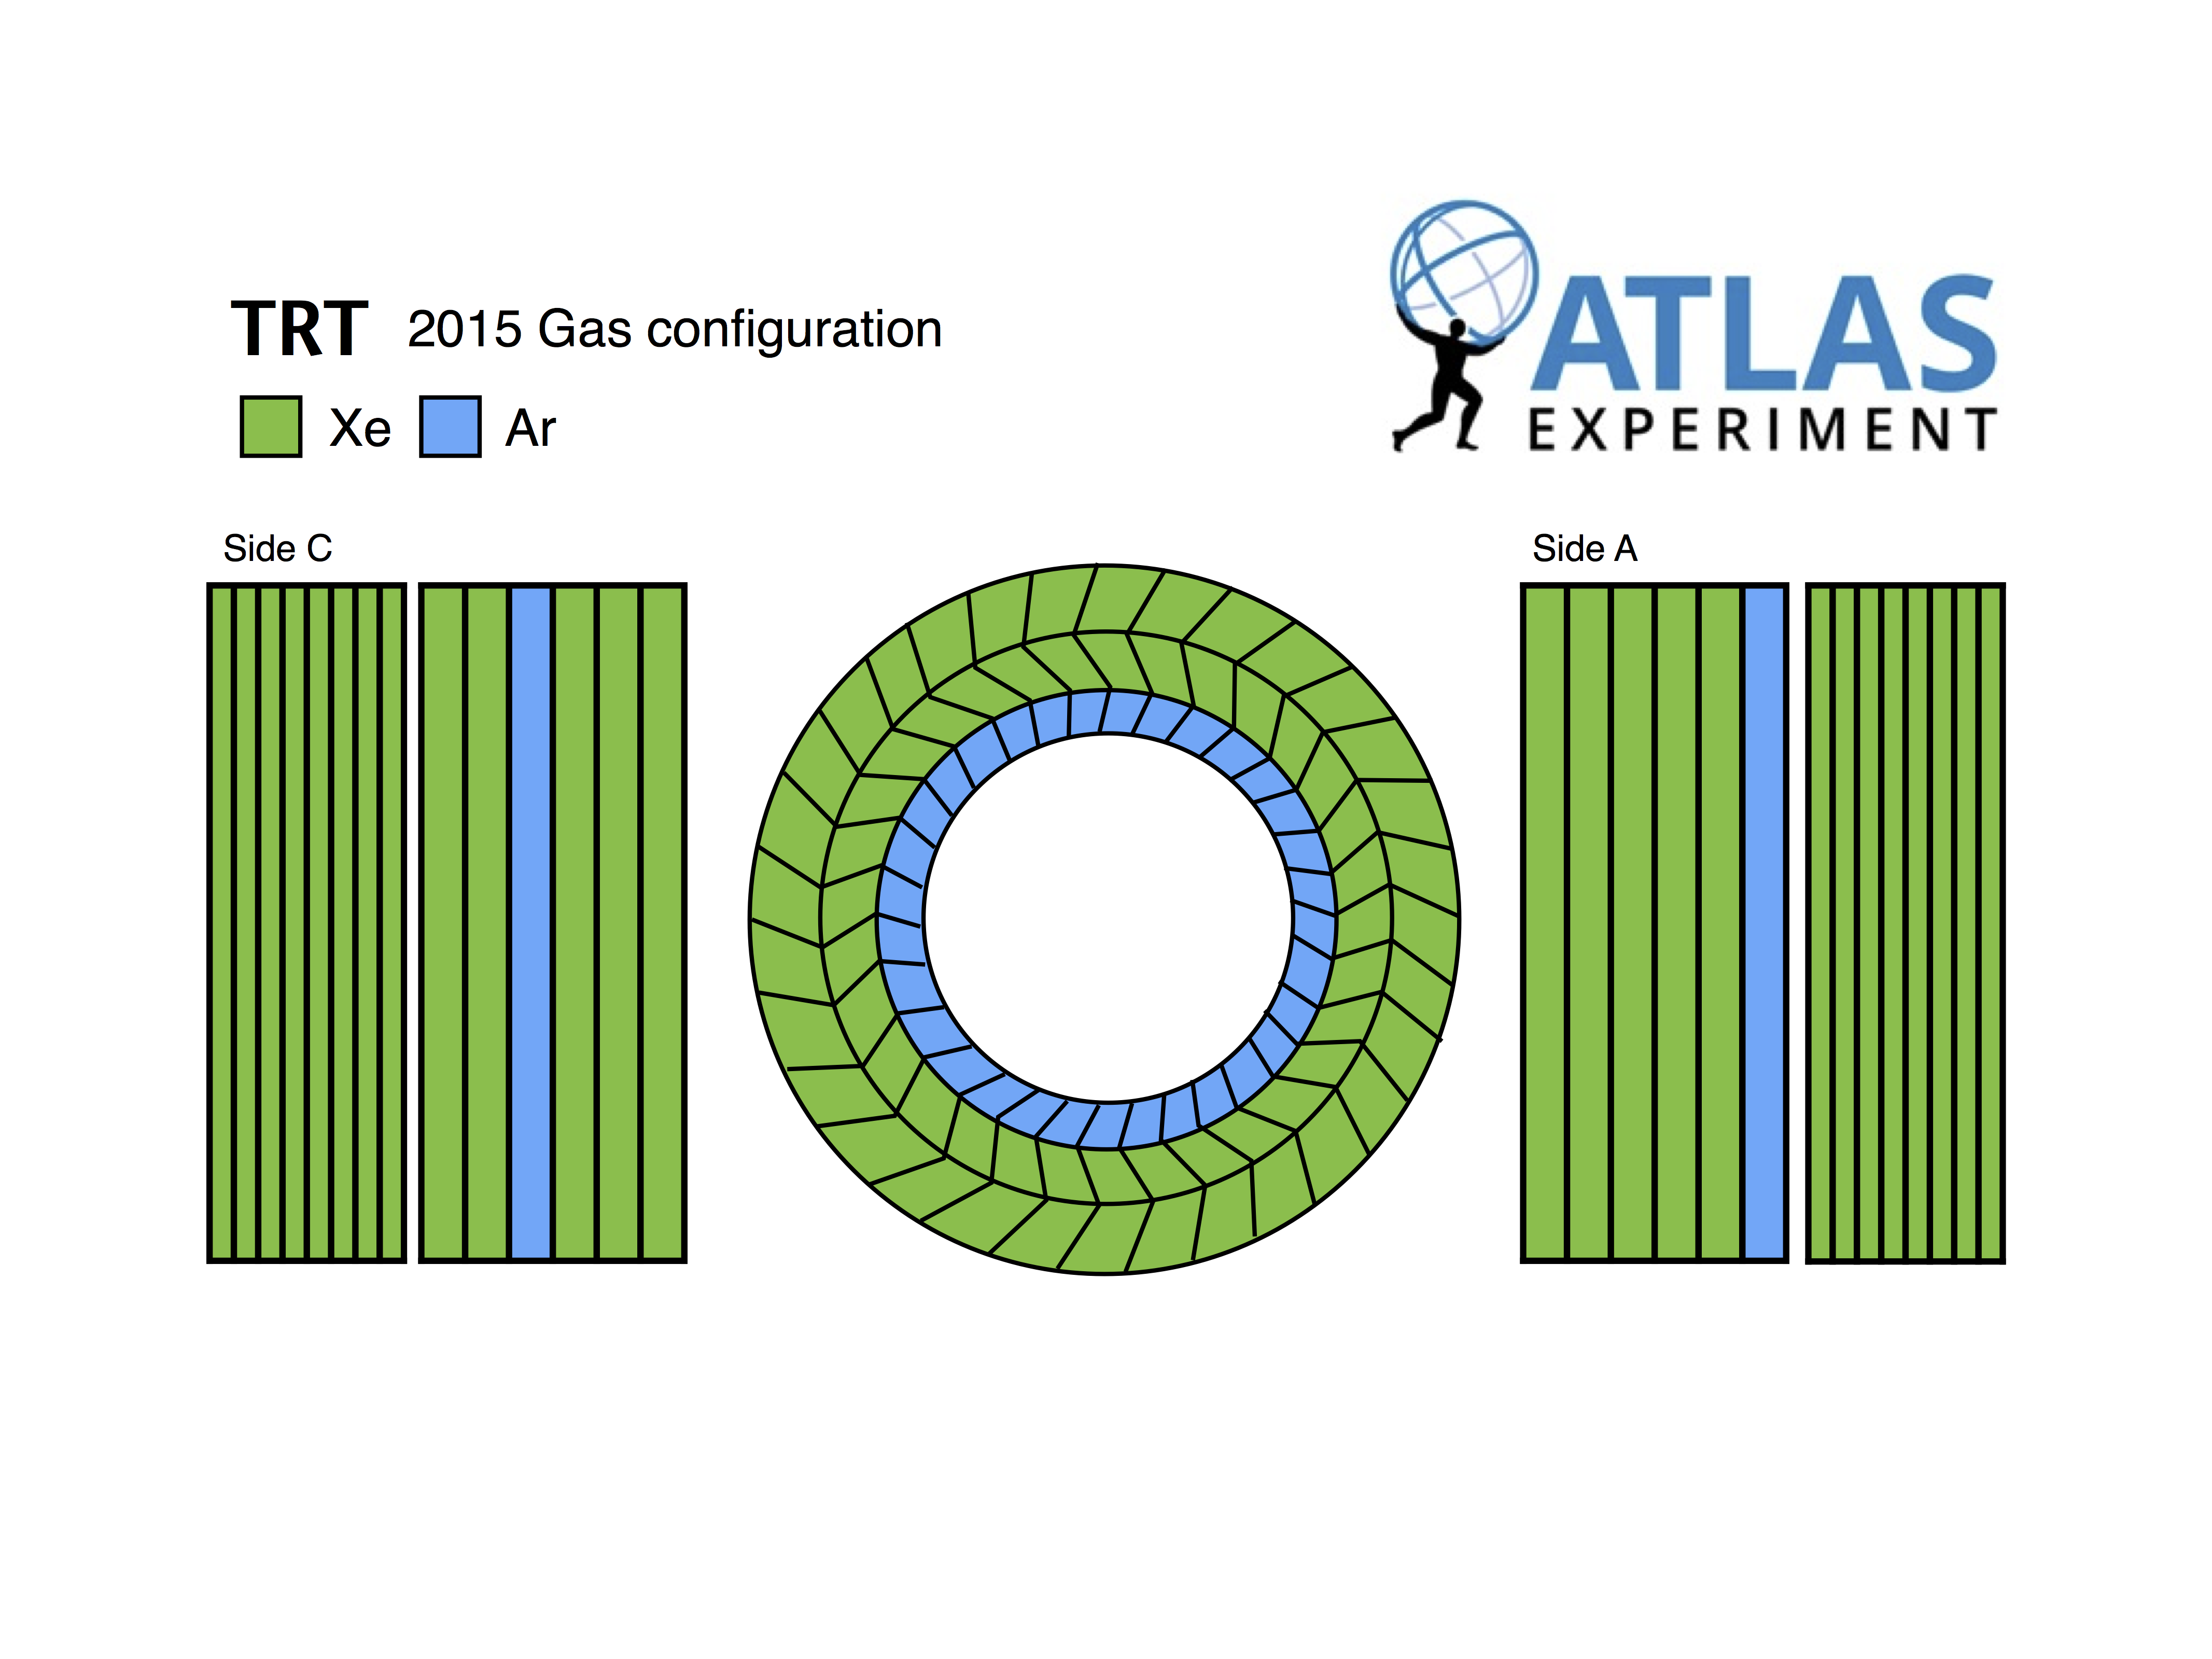
\includegraphics[width=0.9\textwidth]{figures/Detector/trtfig_01.png}
  \caption{}
  \label{chp:det:atlas:trt2015}
\end{subfigure}
\begin{subfigure}{0.5\textwidth}
  \centering
  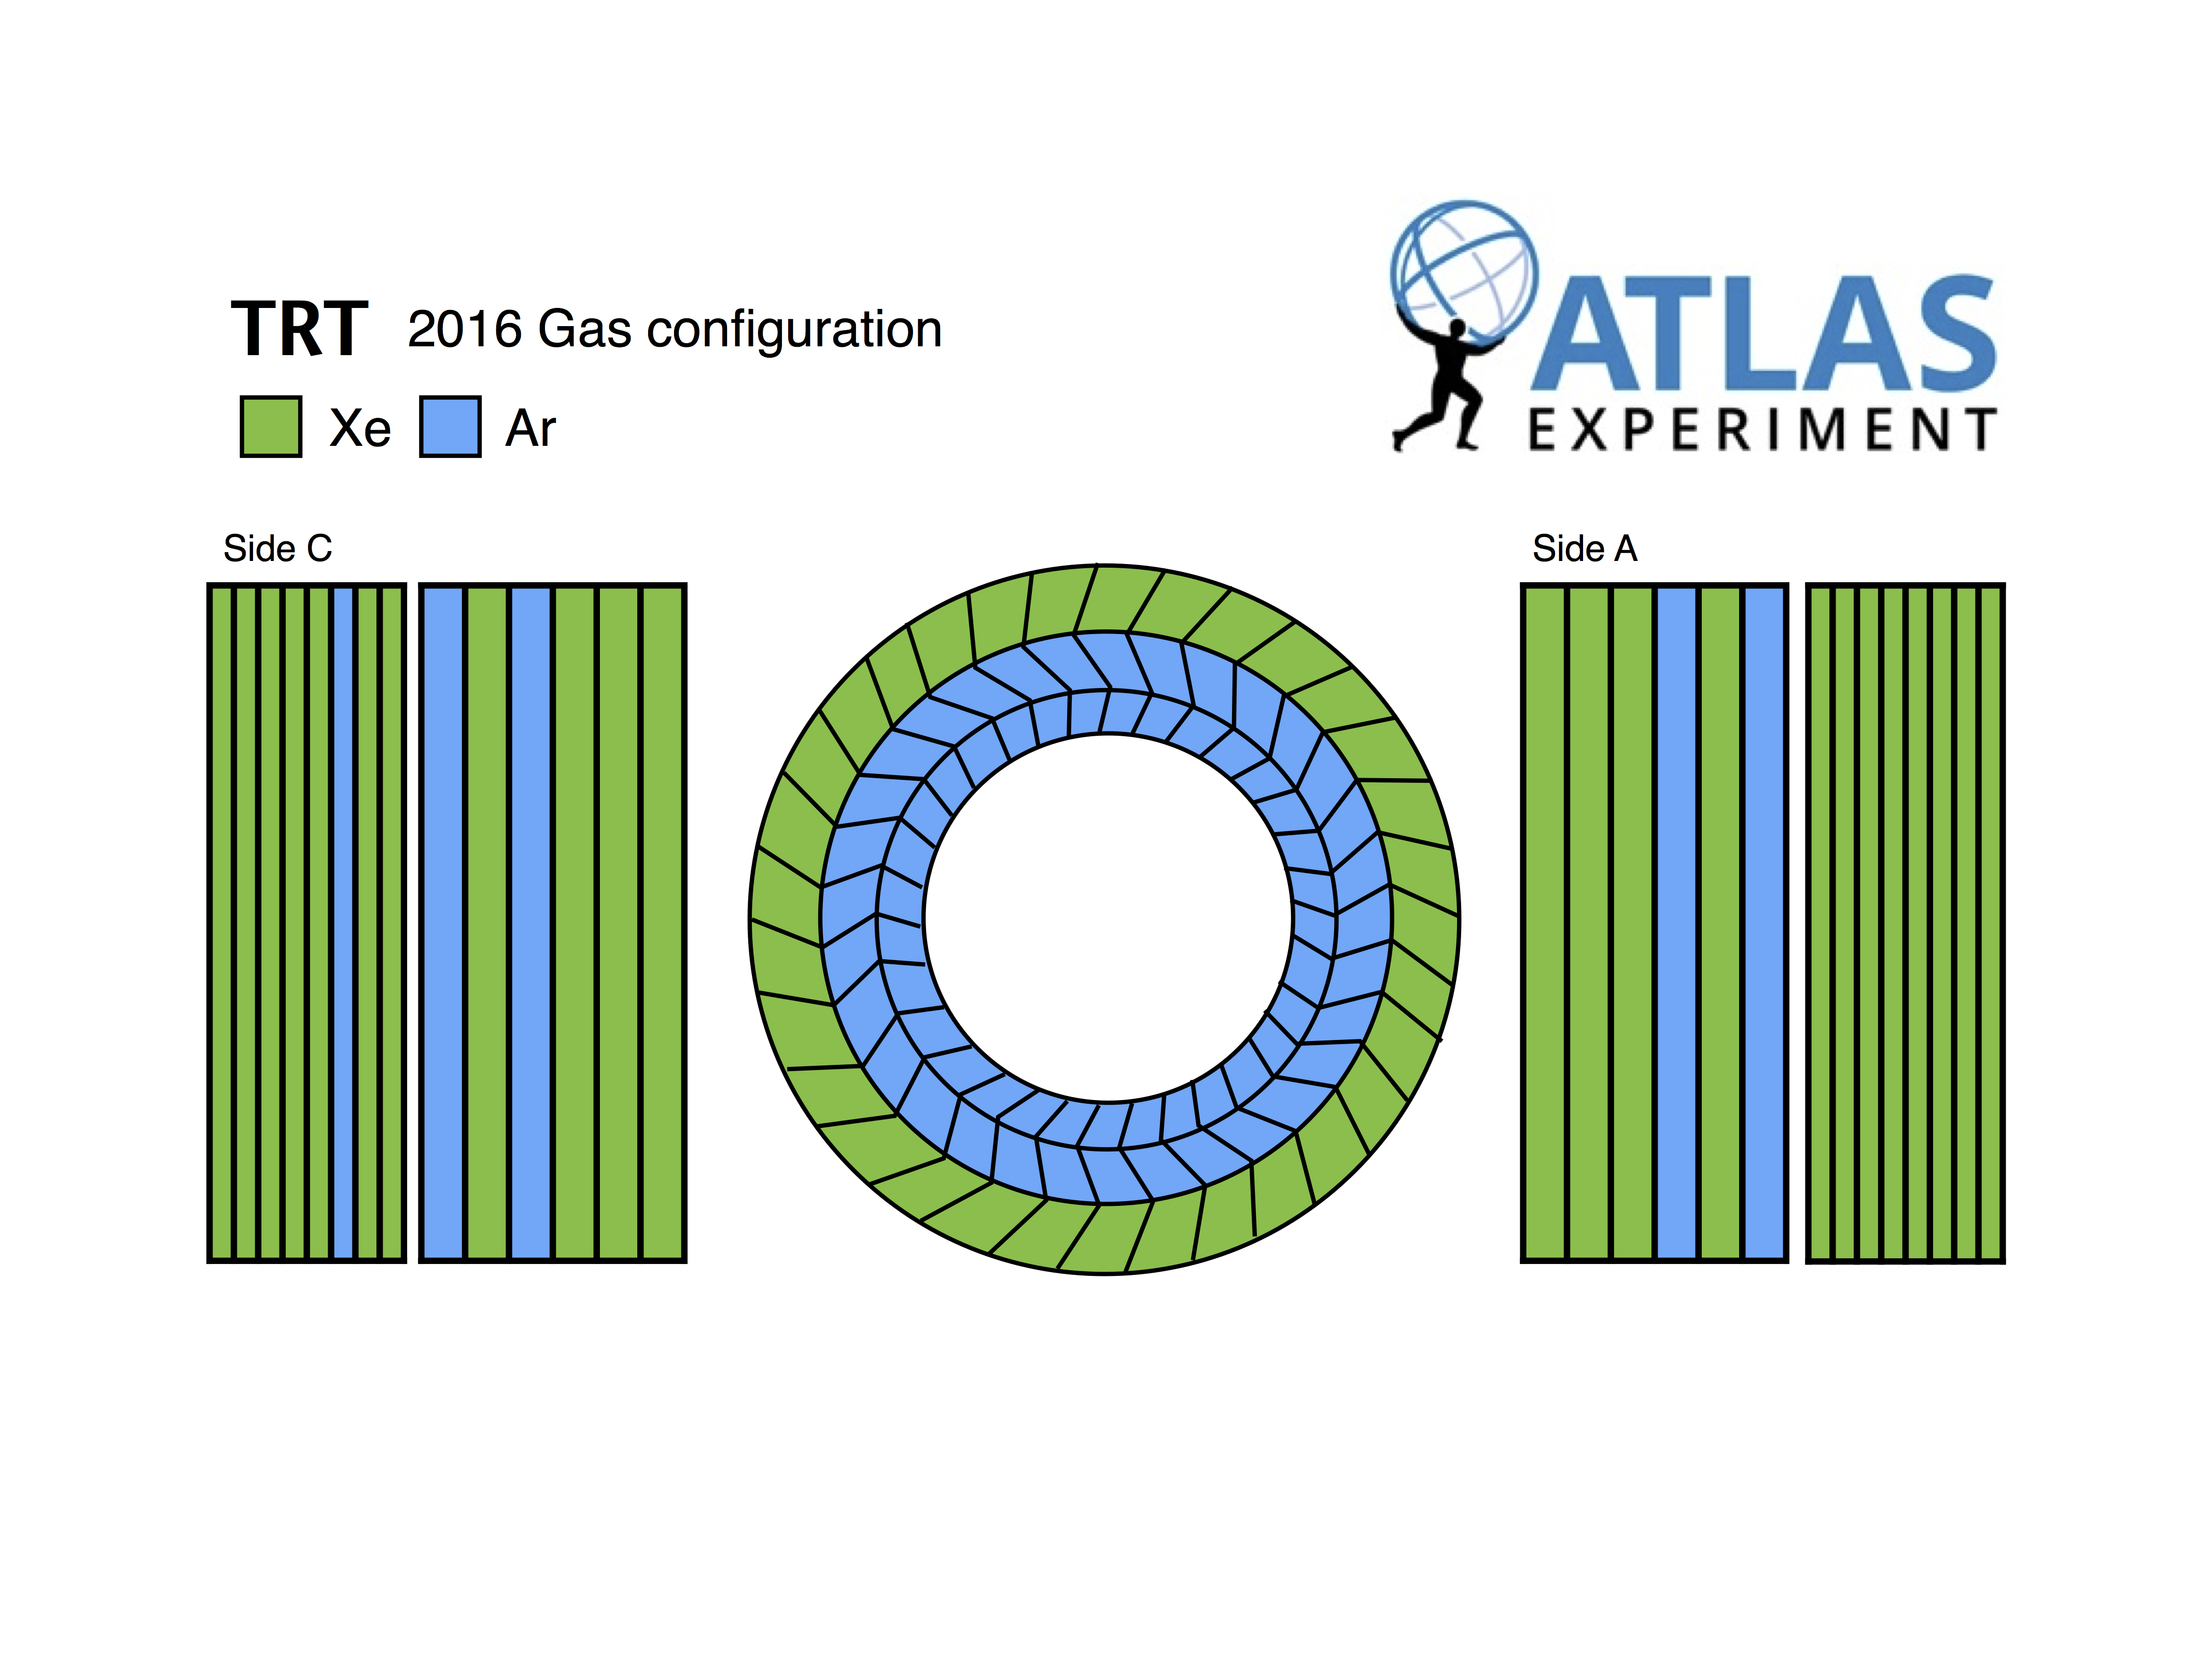
\includegraphics[width=0.9\textwidth]{figures/Detector/trtfig_02.png}
  \caption{}
  \label{chp:det:atlas:trt2016}
\end{subfigure}

\captionsetup{width=0.85\textwidth} \caption{\small TRT gas configuration used in the year (a) 2015 and (b) 2016.}
\label{sec:det:fig:trfgas}
\end{figure}


The spaces between the straws are filled with polymer fibres (barrel) and foils (end-caps) to create transition radiation, which is emitted by highly-relativistic charged particles as they
traverse a material boundary. This effect depends on the Lorentz boost $\gamma$ $(E/m)$ and is strongest for electrons, which means it can be used for particle identification. X-rays coming from the transition radiation process can be absorbed by the noble gas, resulting into additional energy being deposited into the gas. This design  makes the TRT complementary to  the silicon-based tracking devices. Each channel, through the tube drift time measurement, has an intrinsic single-point resolution of $120$ $\mu$m, larger than that of the silicon trackers, but this is compensated by the large number of hits per track (typically more than 30) and the long lever arm.  Furthermore, the high sampling frequency of the wire signals enables the TRT to provide timing information at the nanosecond level.

\subsection{Calorimeters}
The ATLAS calorimeter system \cite{ATLASTDR1} surrounds the ID and it consists of an inner electromagnetic calorimeter and an outer hadronic calorimeter. It was designed to provide full coverage in $\phi$ and to measure a wide range of energy deposits over the entire pseudorapidity coverage of $|\eta|<4.9$ from both neutral and charged particles. The structure of the ATLAS calorimeter is shown in figure \ref{sec:det:fig:ATLASCALO}. In the acceptance region covered by the ID, the granularity of the EM calorimeter is finer in the $\eta$ and $\phi$ directions in order to provide precision measurements of electrons and photons. The rest of the calorimeter system has coarser granularity, yet appropriate for a precise measurement of jet kinematics, and provides sufficient longitudinal containment of the showers  in order to calculate the missing transverse energy.
All of the ATLAS calorimeters are sampling calorimeters; they consist of absorber sheets, which initiate particle showers, alternated with layers of active
medium material to perform energy measurements. When a particle reaches the calorimeter, it produces showers in stages, loosing more and more energy until the shower is completely absorbed. The energy of the initial particle is then obtained by summing up all energy deposits within the active material of the calorimeter. The calorimeter is designed to fully absorb the particle energy to avoid losses caused by escaping particles. It also reduces possible punch-through to the muon chambers by energetic hadrons.

\bfig[t!]
\centering
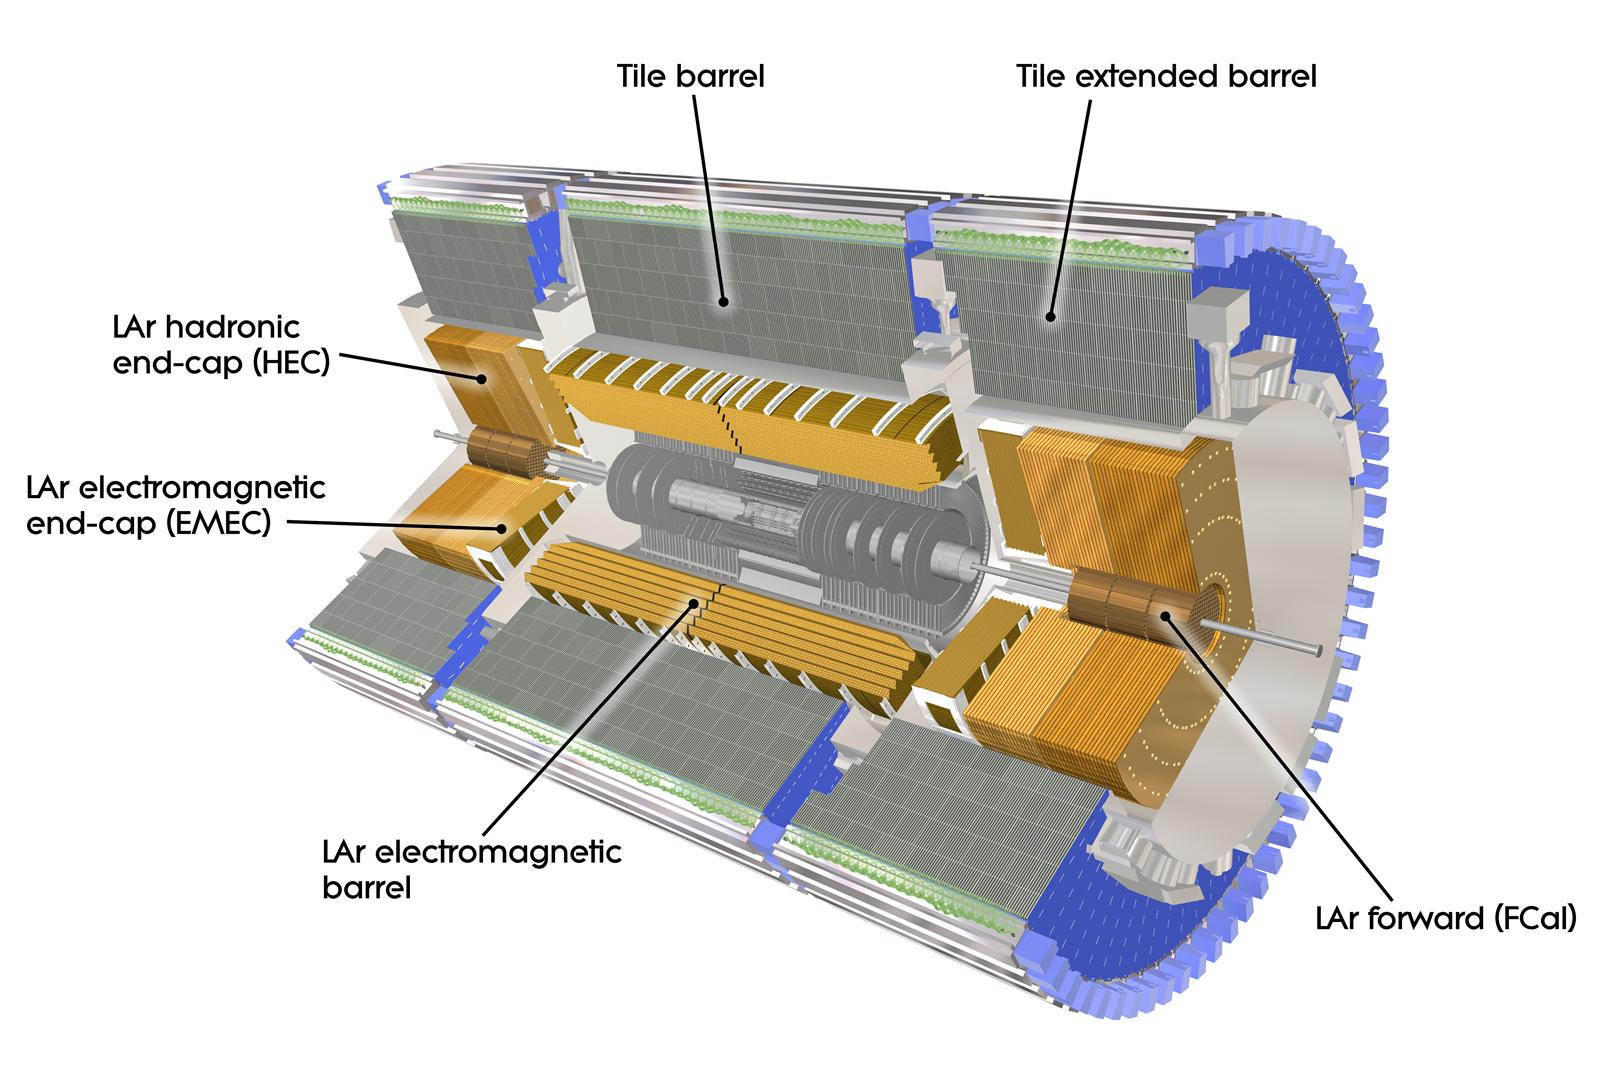
\includegraphics[width=0.8\textwidth]{figures/Detector/calo_all}
\captionsetup{width=0.85\textwidth} \caption{\small Schematic view of the ATLAS calorimeter system.}
\label{sec:det:fig:ATLASCALO}
\efig

\subsubsection{Electromagnetic calorimeter}

The  Electromagnetic CALorimeter (ECAL) is  divided  into  a  barrel  part  ($|\eta|< 1.475$)  and  two  end-caps ($1.375 <|\eta|< 3.2$). The barrel calorimeter consists of two identical half-barrels, separated by a small gap (6 mm) at $z=0$. Each end-cap calorimeter is mechanically divided into two coaxial wheels: an outer wheel covering the region $1.375 <|\eta|< 2.5$, and an inner wheel covering the region $2.5 <|\eta|< 3.2$.
The ECAL uses liquid argon (LAr) as active material with accordion-shaped Kapton electrodes and lead absorber plates over its full coverage. The LAr solution was adopted for its intrinsic linear behaviour, high ionisation yield and stability. The LAr gas is constantly flowing and does not suffer from radiation damage; LAr is therefore preferable in the region close to the interaction point, as well as in the very forward regions. The accordion geometry provides complete $\phi$ symmetry without  azimuthal  cracks.  The  lead  thickness  in  the  absorber  plates  has  been  optimised  as  a function of $\eta$ in terms of EM energy resolution. High voltage is applied between absorber plates to collect ionisation electrons  from the interaction with the LAr as well as to produce signal amplification.
The total thickness of the ECAL is >24~$X_{0}$ in the barrel and >26~$X_{0}$ in the end-caps. This ensures the absorption of electron and photon showers up to few $\tev$ of energy and around 2/3 of typical hadronic showers. Over the region devoted to precision physics ($|\eta|< 2.5$), the ECAL is segmented into three longitudinal sections with different cell structure in the $\eta-\phi$ plane. 
The first layer, which has a constant thickness of $\sim6\,X_{0}$ (upstream material included) as a function of $\eta$, is equipped with narrow readout strips of $\Delta \eta \times \Delta \phi =  0.0031 \times 0.098$.  This  section  acts  as  a  ``preshower''  detector,  enhancing  particle  identification ($\gamma/\pi^{0}, e/\pi$ separation, etc) and providing a precise position measurement in $\eta$. The second layer is  transversally  segmented  into  square  towers  of size $\Delta \eta \times \Delta \phi =  0.025 \times 0.025$  ($\sim 4\times$4 cm$^{2}$ at $\eta=0$). 
The total calorimeter thickness up to the end of the second section is $\sim24$ $X_{0}$, tapered with increasing rapidity (this includes also the upstream material). Combining the information from the first two layers provides a precise measurement of a photon's production vertex. The third layer has a granularity of 0.05 in $\eta$ and a thickness varying between 2 $X_{0}$  and 12 $X_{0}$. For $|\eta|> 2.5$, i.e. for the end-cap inner wheel, the calorimeter is segmented in two longitudinal sections and has a coarser lateral granularity than for the rest of the acceptance. The calorimeter cells point towards the interaction region over the complete eta coverage.  In the region where the amount of material exceeds $\sim2$ $X_{0}$ (as is the case for $|\eta|< 1.8$), a presampler is used to correct for the energy lost by electrons and photons upstream of the calorimeter. The presampler consists of an active LAr layer of thickness 1.1 cm (0.5 cm) in the barrel (end-cap) region. In figure \ref{chp:det:atlas:ATLASECAL} the structure of the ECAL is shown. The total number of channels for the entire ECAL is $\sim$190 000. 
The design energy resolution is:

\be
\frac{\sigma_{E}}{E} = \frac{9\%}{\sqrt{E\,(\gev)}} \oplus 0.3 \%, 
\label{sec:det:eq:ECALresolution}
\ee

\noindent while the angular resolution is $\sigma_\theta \sim 50$ mrad/$\sqrt{E(\gev)}$.


\begin{figure}[t!]
\begin{subfigure}{0.5\textwidth}
  \centering
  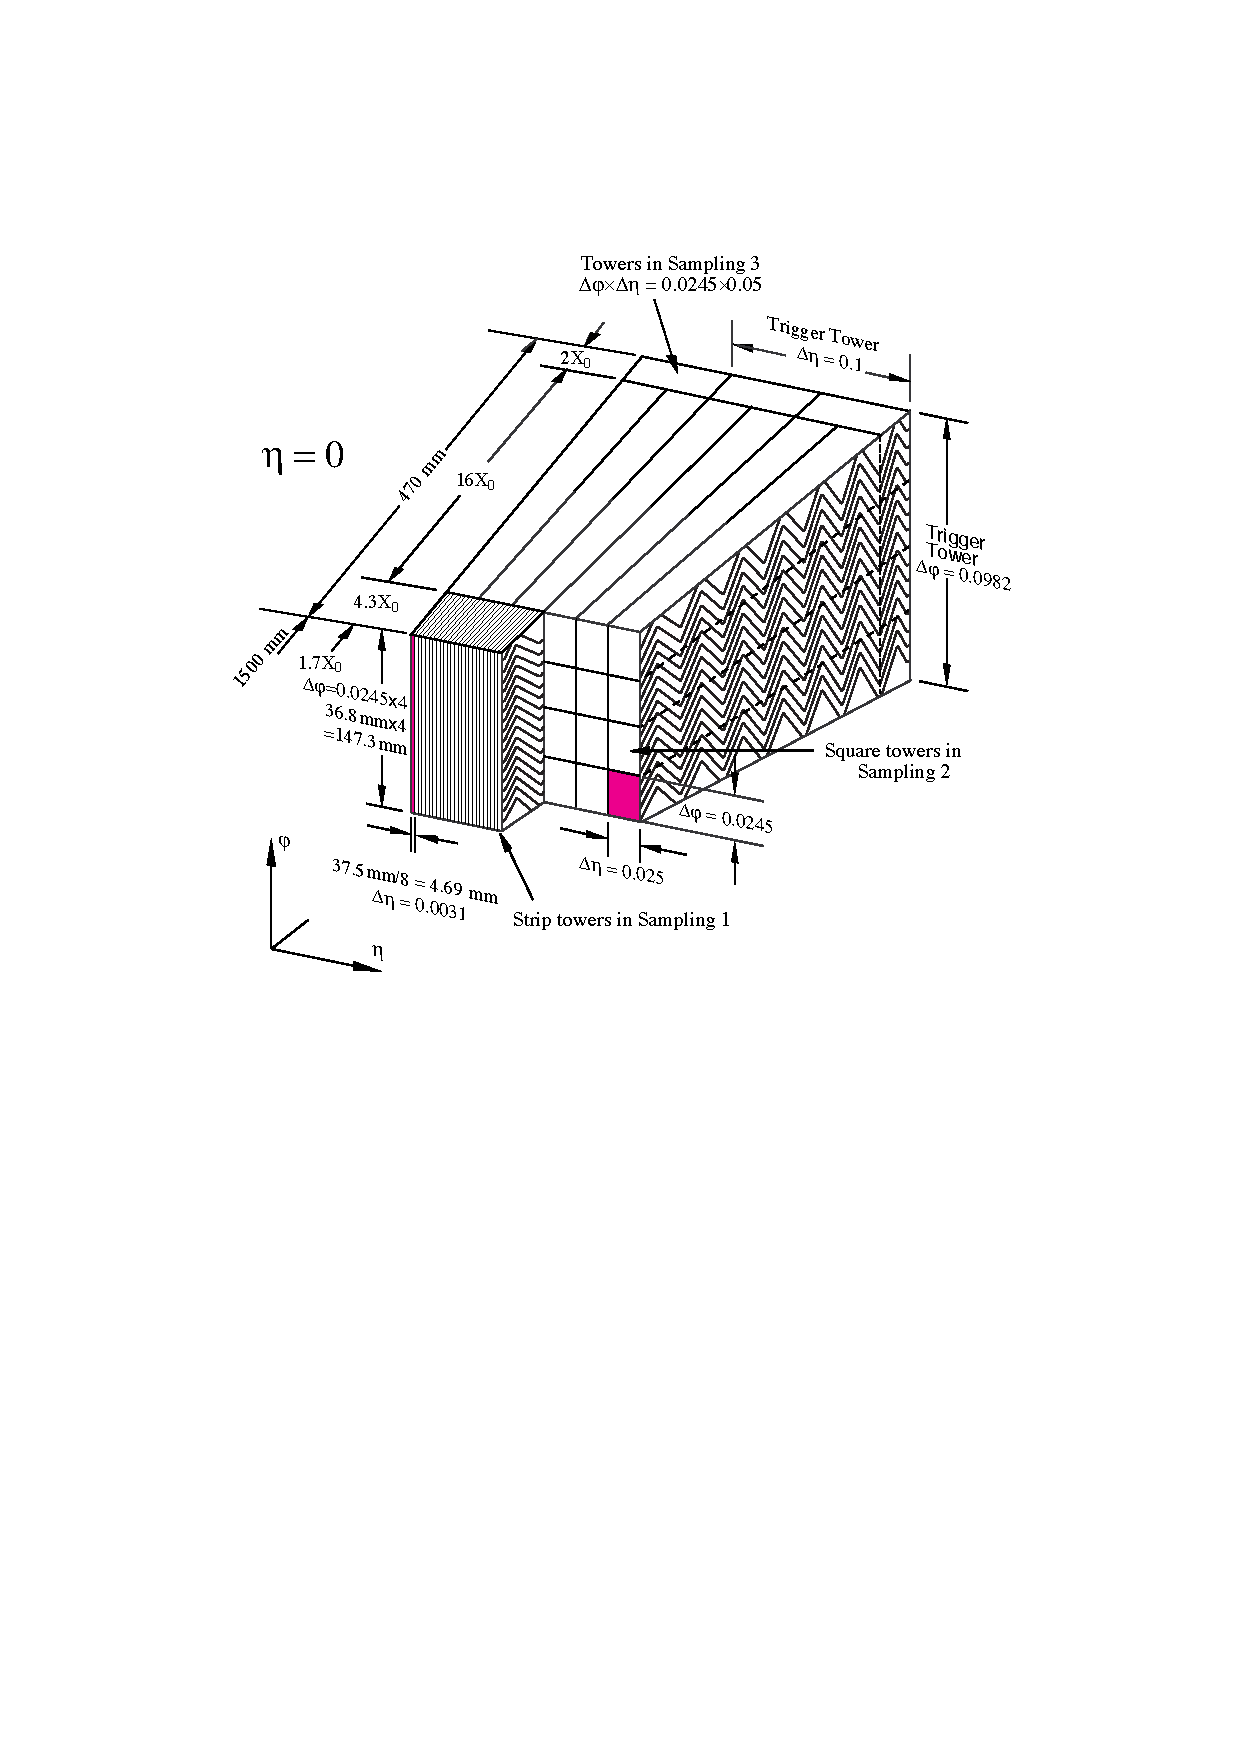
\includegraphics[width=0.9\textwidth]{figures/Detector/larg_module.png}
  \caption{}
  \label{chp:det:atlas:ATLASECAL}
\end{subfigure}
\begin{subfigure}{0.5\textwidth}
  \centering
  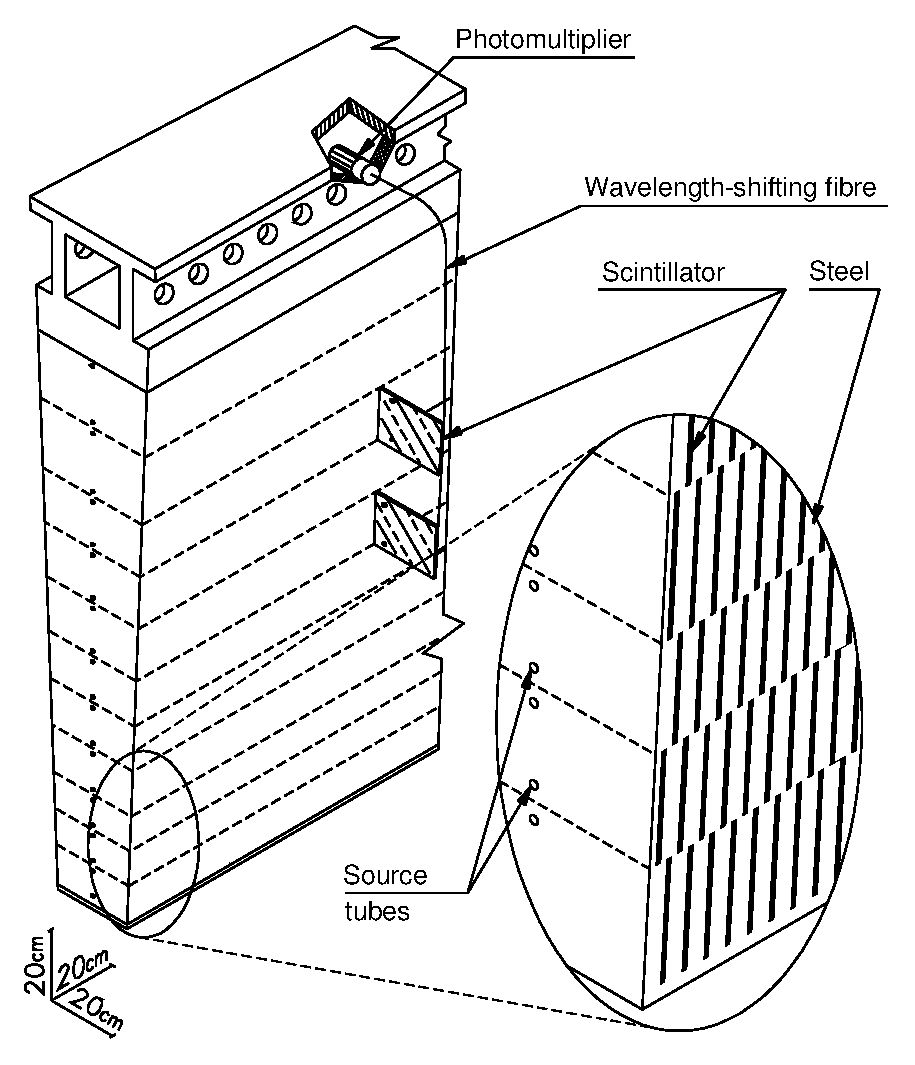
\includegraphics[width=0.8\textwidth]{figures/Detector/TileCal_Module.eps}
  \caption{}
  \label{chp:det:atlas:ATLASTILECAL}
\end{subfigure}

\caption{Schema of different modules of the ATLAS calorimeters: (a) electromagnetic
calorimeter and (b) hadronic calorimeter.}
\label{chp:det:atlas:cal}
\end{figure}



\subsubsection{Hadronic calorimeter}
The ATLAS hadronic calorimeters cover the range $|\eta|< 4.9$ using different techniques best suited for the widely-varying requirements and radiation environment over the large $\eta$ range. An important parameter in the design of the hadronic calorimeter is its thickness: it has to provide good containment for hadronic showers and reduce punch-through into the muon system to a minimum. The total thickness is 11 interaction lengths ($\lambda$) at $\eta = 0$, including about 1.5 $\lambda$ from the outer support, which has been shown both by measurements and simulation to be sufficient to reduce the punch-through well below the irreducible level of prompt or decay muons. Close to 10 $\lambda$ of active calorimeter are adequate to provide good energy resolution for high-energy jets. Together with the large $\eta$ coverage, this also guarantees a good \MET  measurement.
In the central region the Tile calorimeter covers the range $0 < |\eta| < 1.7$ (11.4 m long cylinder with an inner radius 2.28 m and an outer radius of 4.25 m). The Tile calorimeter is composed of one barrel and two extended barrels. It consists of a sampling calorimeter that uses scintillating tiles as the active material and steel as the absorber arranged in three layers. Scintillator tiles, approximately 3 mm in thickness, are arranged radially along the beam pipe with the tile face along the $z$-axis, with steel absorbers sandwiched between the tiles in this orientation. The scintillation light induced in a tile upon the passage of radiation is read out by optical fibres and sent into two separate photomultiplier tubes. Azimuthally, the barrel and extended barrels are divided into 64 modules. In $\eta$, the readout cells, built by grouping fibres into PMTs, are ``pseudo-projective'' towards the interaction region. The resulting granularity is $\Delta \eta \times \Delta \phi =  0.01 \times 0.01$ ($0.2\times0.1$ in the last layer).
The region $1.5< |\eta| < 3.2$ is covered by the Hadronic End-cap Calorimeter (HEC), which uses copper plates as absorbers and LAr as active material for its superior radiation resistance. It  consists of two independent wheels with an outer radius of 2.03 m. Each wheel is built out of 32 identical modules, assembled with fixtures at the periphery, and a central ring. As for the electromagnetic calorimeter, the electric signal produced in the LAr is collected by cathodes on the plates. 
Finally, in the most forward part ($3.1< |\eta| <4.9$) a Forward Calorimeter (FCAL) is present. It is assembled with tungsten rod absorbers embedded in a copper matrix. Between the two, a thin gap filled with LAr provides the active material. The radial depth of the hadronic calorimeter is approximately 7.4 $\lambda$ with minimal variation across the $\eta$ range.  The resolution achieved in this configuration is:
\be
\frac{\sigma_{E}}{E} = \frac{50\%}{\sqrt{E\,\gev}} \oplus 3 \% \text{ for Tile and HEC, and}
\label{sec:det:eq:TILEresolution}
\ee
\be
\frac{\sigma_{E}}{E} = \frac{100\%}{\sqrt{E\,\gev}} \oplus 10 \% \text{ for FCAL.}
\label{sec:det:eq:FCALresolution}
\ee

\subsection{Muon spectrometer}

The ATLAS Muon Spectrometer (MS) \cite{ATLASTDR1} was designed to provide a high-resolution measurement of the muon momentum up to very high energy (few $\tev$) in the pseudorapidity range $|\eta|<2.7$. The muon momentum measurement is based on the muon deflection in the toroidal magnet. The MS can perform measurements in stand-alone mode being independent from other subdetectors; this feature is important for fast event triggering as well as for the redundancy of the pattern recognition. The MS employs four different technologies in order to fulfil the different needs of the detector: two different precision tracking chambers for precise momentum measurements and two different triggering chambers (with fast response time <25 ns) used to provide a trigger signal and timing calibration to the event. Different technologies have been also adopted in order to keep similar performance in terms of radiation hardness, low occupancy and detector efficiency since the particle flux from the interaction point has a large variation according to the position of the muon chambers. In the barrel region, chambers are arranged in three cylindrical layers around the beam axis, one layer being inside the magnet. In the end-caps these three layers are placed on four wheels perpendicularly to the beam axis. The conceptual layout of the MS is shown in figure \ref{sec:det:fig:ATLASMuon}. The total number of channels for the entire MS is $\sim$1 million. 

\bfig[htb!]
\centering
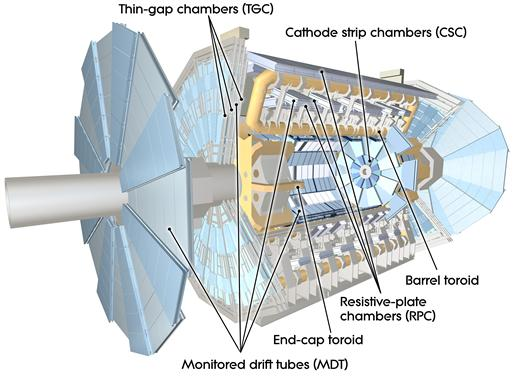
\includegraphics[width=0.8\textwidth]{figures/Detector/muons}
\captionsetup{width=0.85\textwidth} \caption{\small Schematic view of the ATLAS muon spectrometer.}
\label{sec:det:fig:ATLASMuon}
\efig

\subsubsection{Tracking chambers}

\bi
\ib \textbf{MDT} (Monitored Drift-Tube Chambers): MDTs are proportional chambers based on the drift tube technology. The tubes of 30 mm diameter are made of aluminium with a 50 $\mu$m diameter central W-Re wire. The tubes are operated with a non-flammable mixture of $93\,\%$ Ar and $7\,\%$ CO$_{2}$ at 3 bar absolute pressure; the chosen working point provides for a non-linear space-time relation with a maximum drift time of 700 ns, a small Lorentz angle, and excellent ageing properties. To improve the resolution of a chamber beyond the single-wire limit (80 $\mu$m) and to achieve adequate redundancy for pattern recognition, the MDT chambers are constructed from $2\times4$ monolayers of drift tubes for the inner station, and $2\times3$ monolayers for the middle and outer stations. The tubes are arranged in multilayer pairs of three or four monolayers, respectively, on opposite sides of a rigid support structure and placed transverse to the beam axis. A chamber provides a resolution of 40 $\mu$m, while the resolution for three layers of MDTs is 30 $\mu$m. Due to their reliability, mechanical robustness and simpler operation, MDT chambers are employed to cover the larger area of the spectrometer ($|\eta|$<2.7, 2.0 for the innermost layer).

\ib \textbf{CSC} (Cathode Strip Chambers): CSCs are multiwire proportional chambers  with cathode strip readout and with a symmetric cell in which the anode-cathode spacing is equal to the anode wire pitch. The precision coordinate is obtained by measuring the charge induced on the segmented cathode by the avalanche formed on the anode wire. The spatial resolution is $\sim40$ $\mu$m in the bending plane and $\sim$5 mm in the non-bending one. The maximum drift time for signal collection is 40 ns compared to the 700 ns of the MDTs; this gives the possibility to achieve higher acquisition rates. Due to this capability, together with the high radiation resistance, CSCs are used in the range $2.0< |\eta| <2.7$. The baseline CSC gas is a non-flammable mixture of $30\,\%$ Ar, $50\,\%$ CO$_{2}$, and $20\,\%$ CF$_{4}$; the fact that this gas contains no hydrogen  explains the low sensitivity to neutron backgrounds.
\ei


\subsubsection{Triggering chambers}

\bi

\ib\textbf{RPC} (Resistive Plate Chambers): RPCs are gaseous detectors providing a space-time resolution of 1 cm$\times$1 ns allowing single bunch-crossing discrimination. The basic RPC unit is a narrow gas gap filled with a gas mixture ($94.7\,\%$ C$_{2}$H$_{2}$F$_{4}$, $5\,\%$ Iso-C$_{4}$H$_{10}$, and $0.3\,\%$ SF$_{6}$) and formed by two parallel resistive bakelite plates.  The signal is read out via capacitive coupling by metal strips on both sides of the detector. A trigger chamber is made from two rectangular detector layers, each one read out by two orthogonal series of pick-up strips, one parallel to MDT wires and the other orthogonal to the MDT wires. RPCs provide also the $\phi$ coordinate for the tracks in the final analysis since MDTs only give the $\eta$ coordinate.

\ib\textbf{TGC} (Thin Gap Chambers): TGCs are similar to multiwire chambers with the only difference being that the anode wire pitch is larger than the cathode-anode distance. The chambers operate with a highly-quenching gas mixture of $55\,\%$ CO$_{2}$ and $45\,\%$ n-pentane (n-C$_{5}$H$_{12}$) and with wires  arranged parallel to the MDT wires provide the trigger information. They are assembled in the end-cap wheels, covering the region $1.05<|\eta|<2.7$ ($1.05<|\eta|<2.4$ for triggering). The timing resolution is comparable to the RPC's one while the spatial resolution is in the range of 2-7 mm for both coordinates.

\ei

In the barrel region, muon tracks are measured with MDT chambers and RPCs assembled on three cylindrical layers: the coordinate in the bending plane is provided by the MDT chambers, while the coordinate in the non-bending plane is provided by the RPCs (together with timing information). In the end-cap region, MDT and CSC provide the coordinate in the bending plane while the non-bending coordinate is provided by the TGCs. The muon spectrometer is designed to measure in standalone mode muons with \pt\ down to 3 $\gev$ (softer muons are stopped) and up to a few $\tev$. The momentum resolution achieved is $\sim10\%$ at $p_{T}= 1$ $\tev$. At lower energies the resolution is improved substantially by combining the track reconstructed in the muon spectrometer with a track reconstructed in the ID.
During LS1 the MS was improved targeting an increased muon acceptance. Completion of the spectrometer acceptance was already foreseen for this shutdown period, with new resistive plate chambers (RPC) placed in the barrel holes due to the toroid feet and elevators ($+2.8\%$ acceptance) and extra end-cap chambers.

\subsection{Luminosity detectors}

A good determination of the integrated luminosity is of particular importance to reach the ultimate precision in measurement of processes of interest. The luminosity in a $pp$ collider, $\lag$, defined in equation \ref{sec:det:eq:lumi}, can be expressed as well as:

\be
\lag = \frac{\mu_{\rm vis}n_{b}f_{\rm rev}}{\sigma_{\rm vis}},
\label{sec:det:eq:lumidect}
\ee

\noindent where $f_{\rm rev}$ is the collider revolution frequency, $n_{b}$ is the number of colliding bunches, and $\sigma_{\rm vis}$ is the visible inelastic cross section (total inelastic cross section times the detector acceptance and efficiency). The visible interaction rate per bunch crossing is denoted by $\mu_{\rm vis}$. It is extracted primarily from the signals coming from specific luminosity detectors. The simplest algorithm consists in simple counting of ``bunch crossings'' where detectors reported a signal, but more refined algorithms are used, in particular when the pileup contamination is no longer negligible. In order to use the measured $\mu_{\rm vis}$ for luminosity determination, each detector and algorithm must be calibrated by determining its visible cross section $\sigma_{\rm vis}$. Van der Meer scans allow to determine the effective beam size as well as the maximum achievable collision rate. These are special low-intensity LHC runs where the beam separation in the transverse planes is varied (scanned) in order to determine the beams' overlap profile.

The main detectors for luminosity measurement are listed below:
\bi

\ib \textbf{LUCID-2} (LUminosity measurements using Cherenkov Integrating Detector): It consists of 16+16 10 mm diameter Cerenkov detectors for luminosity measurements. LUCID-2 uses the thin quartz windows of photomultipliers as Cherenkov medium. To monitor the gain stability of  the photomultipliers, small sources of radioactive Bi-207 are deposited on to the quartz windows. The luminosity is measured  by not only counting hits (signals over threshold) in the detectors but also by integrating the signals. LUCID-2 is the only detector in ATLAS that can measure luminosity for individual bunches by charge integration.

\ib \textbf{BCM} (Beam Conditions Monitor): It consists of 1 cm$^{2}$ diamond detectors located at $z = 184$ cm around the beam pipe. Their fast readout and good time resolution (0.7 ps) allow them to provide luminosity information for each bunch crossing. At the same time, they are also employed to trigger on beam losses and induce the dump of the beam, thus protecting the silicon detectors from damage that might result from an uncontrolled beam.

\ib \textbf{ALFA} (Absolute Luminosity For ATLAS): It consists of eight scintillating fibers detectors placed at 240 m from the interaction point inside roman pots, above and below the beam pipe. It is a subdetector that is only activated during special runs.

\ei
In addition, cross-checks of the luminosity measurement have been performed using information from other standard subdetectors: counting of primary vertices reconstructed by the ID, and integrated signals from the Tile and forward calorimeters. The precision achieved is of a few $\%$ depending on the data-taking year.

\subsection{Trigger and data acquisition system}

Due to technical and practical limitations, not every LHC collision can be recorded by the ATLAS detector. The goal of the ATLAS trigger and data acquisition (DAQ) system is to select in real time and to record efficiently events with interesting characteristics for physics analyses. The implementation results in a multi-level system optimised to cope with the very high interaction rate and short bunch spacing of the LHC. The ATLAS trigger system is shown schematically in figure \ref{sec:det:fig:ATLASTrigger}.\par
The trigger system consists of a hardware Level 1 (L1) and a single software-based high-level trigger (HLT). This two-stage system will reduce the event rate from the bunch-crossing rate of 40 MHz to 100 kHz at L1 and to an average recording rate of 1 kHz at the HLT. During Run 1, this was a three-stage system with two stages in the HLT. In Run 2 the Event Builder and Event Filter farms are merged into a unique HLT farm for simplification and dynamic resource sharing \cite{DAQTDR}.  At L1, fast custom-made electronics find regions of interest (RoI) using the calorimeter and muon data with coarse information within a latency of 2.5 $\mu$s and keeps the information in pipeline memories. High-$\pt$ muons are identified using only the trigger chambers, RPCs in the barrel, and TGCs in the end-caps. The calorimeter selections  are  based  on  reduced-granularity  information  from  all  the  calorimeters. 
The L1 system in Run 2 consists of the L1 calorimeter trigger system (L1Calo), the L1 muon trigger system (L1Muon), new L1 topological trigger modules (L1Topo) that allow to select events on topological quantities between L1 objects within the L1 latency, and the Central Trigger Processors (CTP). 
At the HLT, fast algorithms accessing data from an RoI, or offline-like algorithms using the full-event information, run on a unique PC farm within a processing time of 0.2 s on average. At the end of 2016, a hardware track finder (FTK) is planned to be fully integrated and will provide tracks to the HLT at the L1 rates. 

\bfig[h!]
\centering
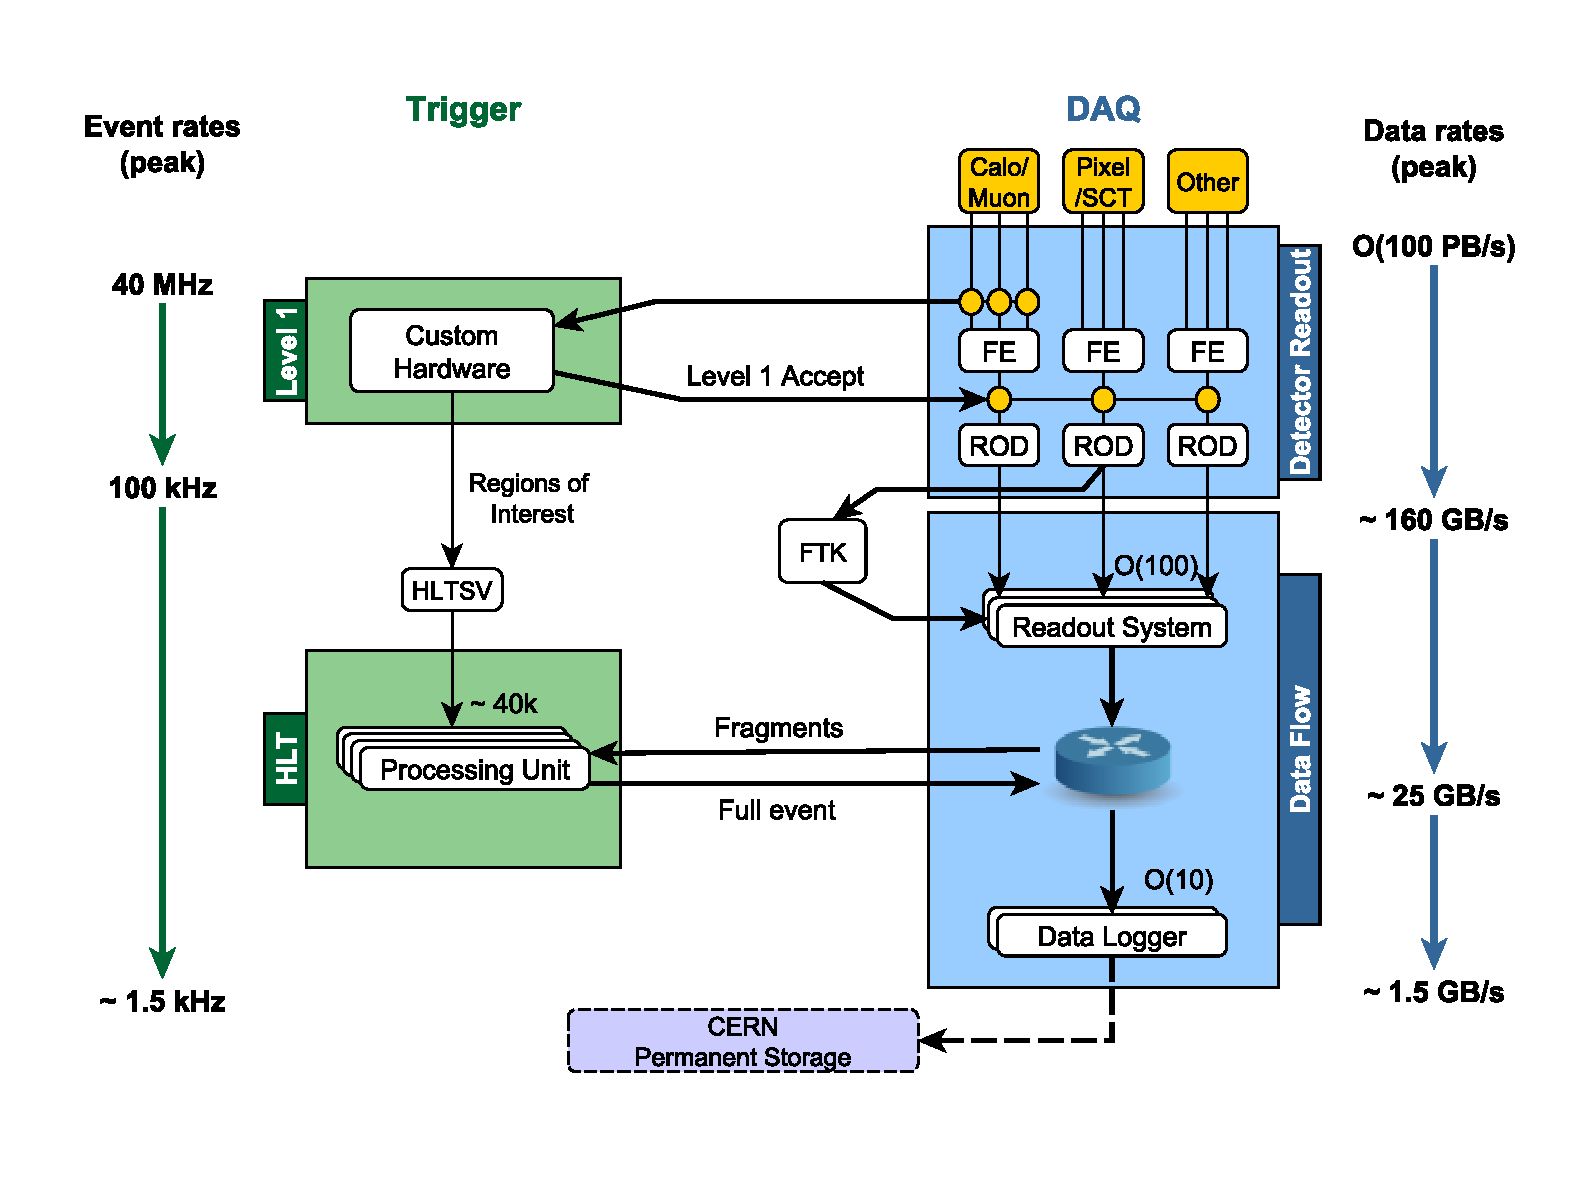
\includegraphics[width=0.82\textwidth]{figures/Detector/tdaqFullNew2016.pdf}
\captionsetup{width=0.85\textwidth} \caption{\small Schematic view of the ATLAS trigger system showing output rates in Run 2.}
\label{sec:det:fig:ATLASTrigger}
\efig


Most of the trigger chains used for physics are unscaled, meaning that all the events passing the selection are kept. Other trigger chains that contain either too many events or events considered not physically interesting are prescaled. These are characterised by a prescaling value, $P$, meaning that of all the events that activated the trigger, only 1/$P$ are accepted. These trigger chains are usually used for checks or calibration rather than physics analysis.
The term trigger chain refers to the sequence of selections that define a certain trigger object. The naming convention is:

\be
\textrm{[LEVEL][N][TYPE(S)][THRESHOLD][ISOLATION][QUALITY]},
\label{sec:det:eq:trig}
\ee


\noindent where the components, from left to right, are: the trigger level used, the multiplicity of the type, the object candidate, the threshold applied to the transverse momentum or energy of the object candidate, the object isolation, and the severity of the final algorithm requirements. Trigger chains define a trigger menu, where they are associated to their prescale value, and which is chosen based on the physics program of the data-taking period and depending on the LHC instantaneous luminosity.

\subsection{ATLAS operation}
\label{sec:det:sub:op}

The integrated luminosity for each of the two years of Run 2 is reported in figure \ref{sec:det:fig:ATLASLumi}.
The luminosity delivered by the LHC machine is shown in green while the amount of luminosity collected by the ATLAS detector is reported in yellow. The inefficiency in the data taking arises partly from the so-called ``warm start'' procedure, which consists in ramping up the voltages for the silicon detector only after the LHC has declared stable beam, or due to transient problems in the trigger and detector data acquisition. The ATLAS data-taking efficiency was above $90\%$ in both years. \par The fraction of good data delivered by each subdetector is shown in figure \ref{sec:det:fig:ATLASDQ} for both data-taking years in Run 2 so far. The fraction is $\sim90\%$ in each year; table \ref{sec:det:tab:atlum} summarises the integrated luminosity collected by ATLAS and  flagged as ``good quality data'' from all the subdetectors. For the measurements presented in this dissertation, all ATLAS subdetectors are needed, as the physics objects used in the analyses are reconstructed using the information from the full detector. The fraction of data considered was collected in the full 2015 and until July 2016, giving a total integrated luminosity of 13.2 fb$^{-1}$ at $\sqrt{s}=13$ $\tev$ satisfying data-quality requirements.

\begin{figure}[t!]
  \begin{subfigure}{0.5\textwidth}
  \centering
  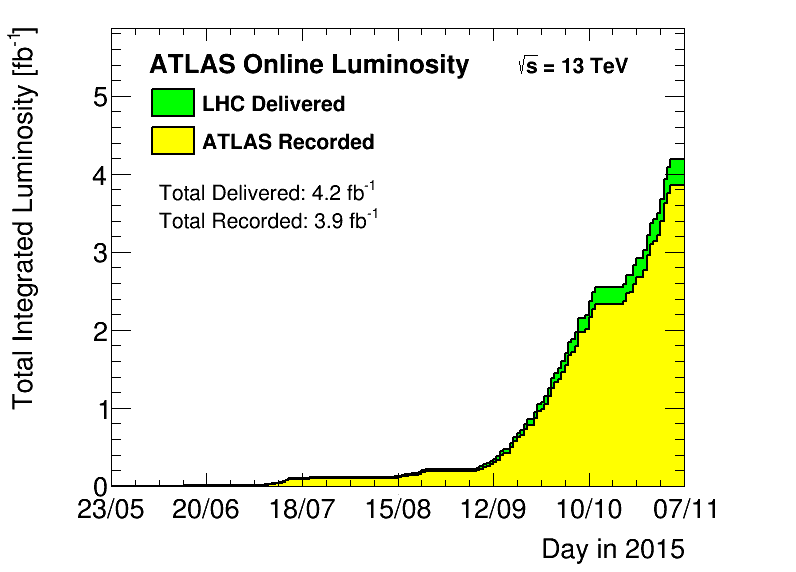
\includegraphics[width=0.9\textwidth]{figures/Detector/Lumi2015.png}
  \captionsetup{width=0.85\textwidth} \caption{\small }
  \label{sec:det:fig:lumi15}
\end{subfigure}
\begin{subfigure}{0.5\textwidth}
  \centering
  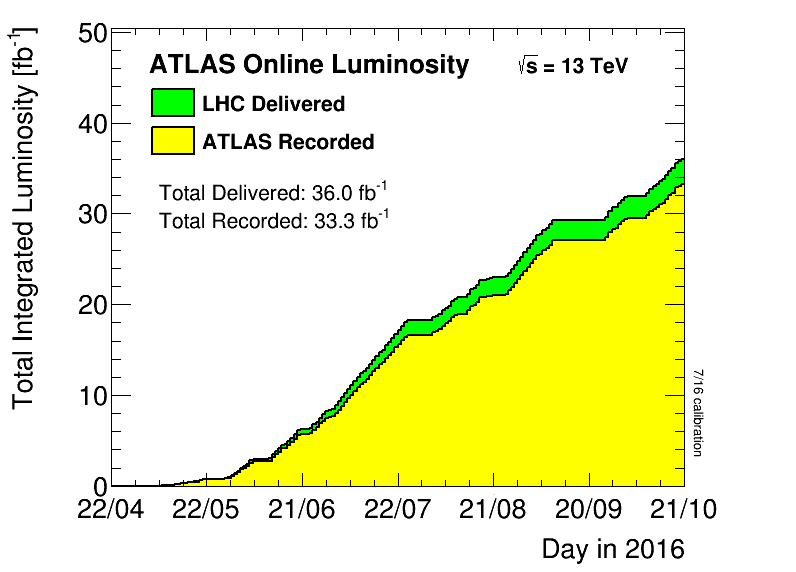
\includegraphics[width=0.9\textwidth]{figures/Detector/Lumi2016.png}
  \captionsetup{width=0.85\textwidth} \caption{\small }
  \label{sec:det:fig:lumi16}
\end{subfigure}

\captionsetup{width=0.85\textwidth} \caption{\small Integrated luminosity delivered by the LHC in the years (a) 2015 and (b) 2016 as a function of time. Also shown is the integrated luminosity recorded by ATLAS.}
\label{sec:det:fig:ATLASLumi}
\end{figure}


\bfig[b!]
\centering
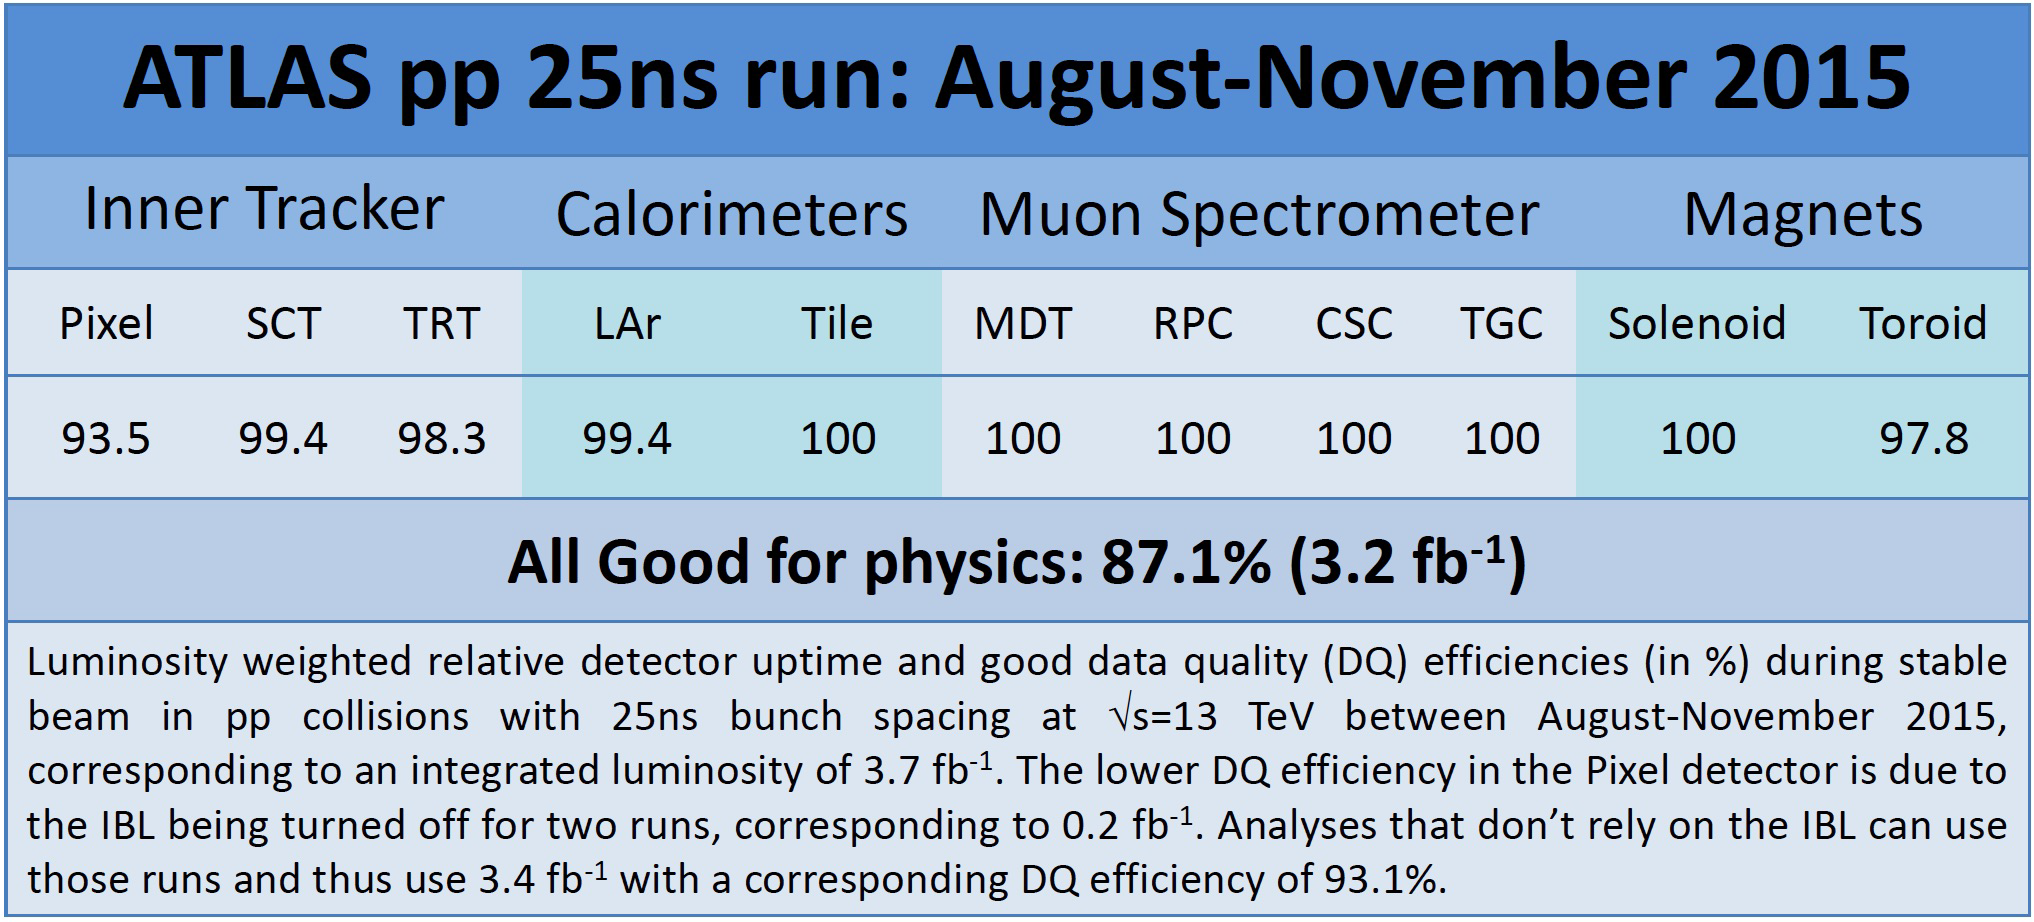
\includegraphics[width=0.85\textwidth]{figures/Detector/DQ2015.png}
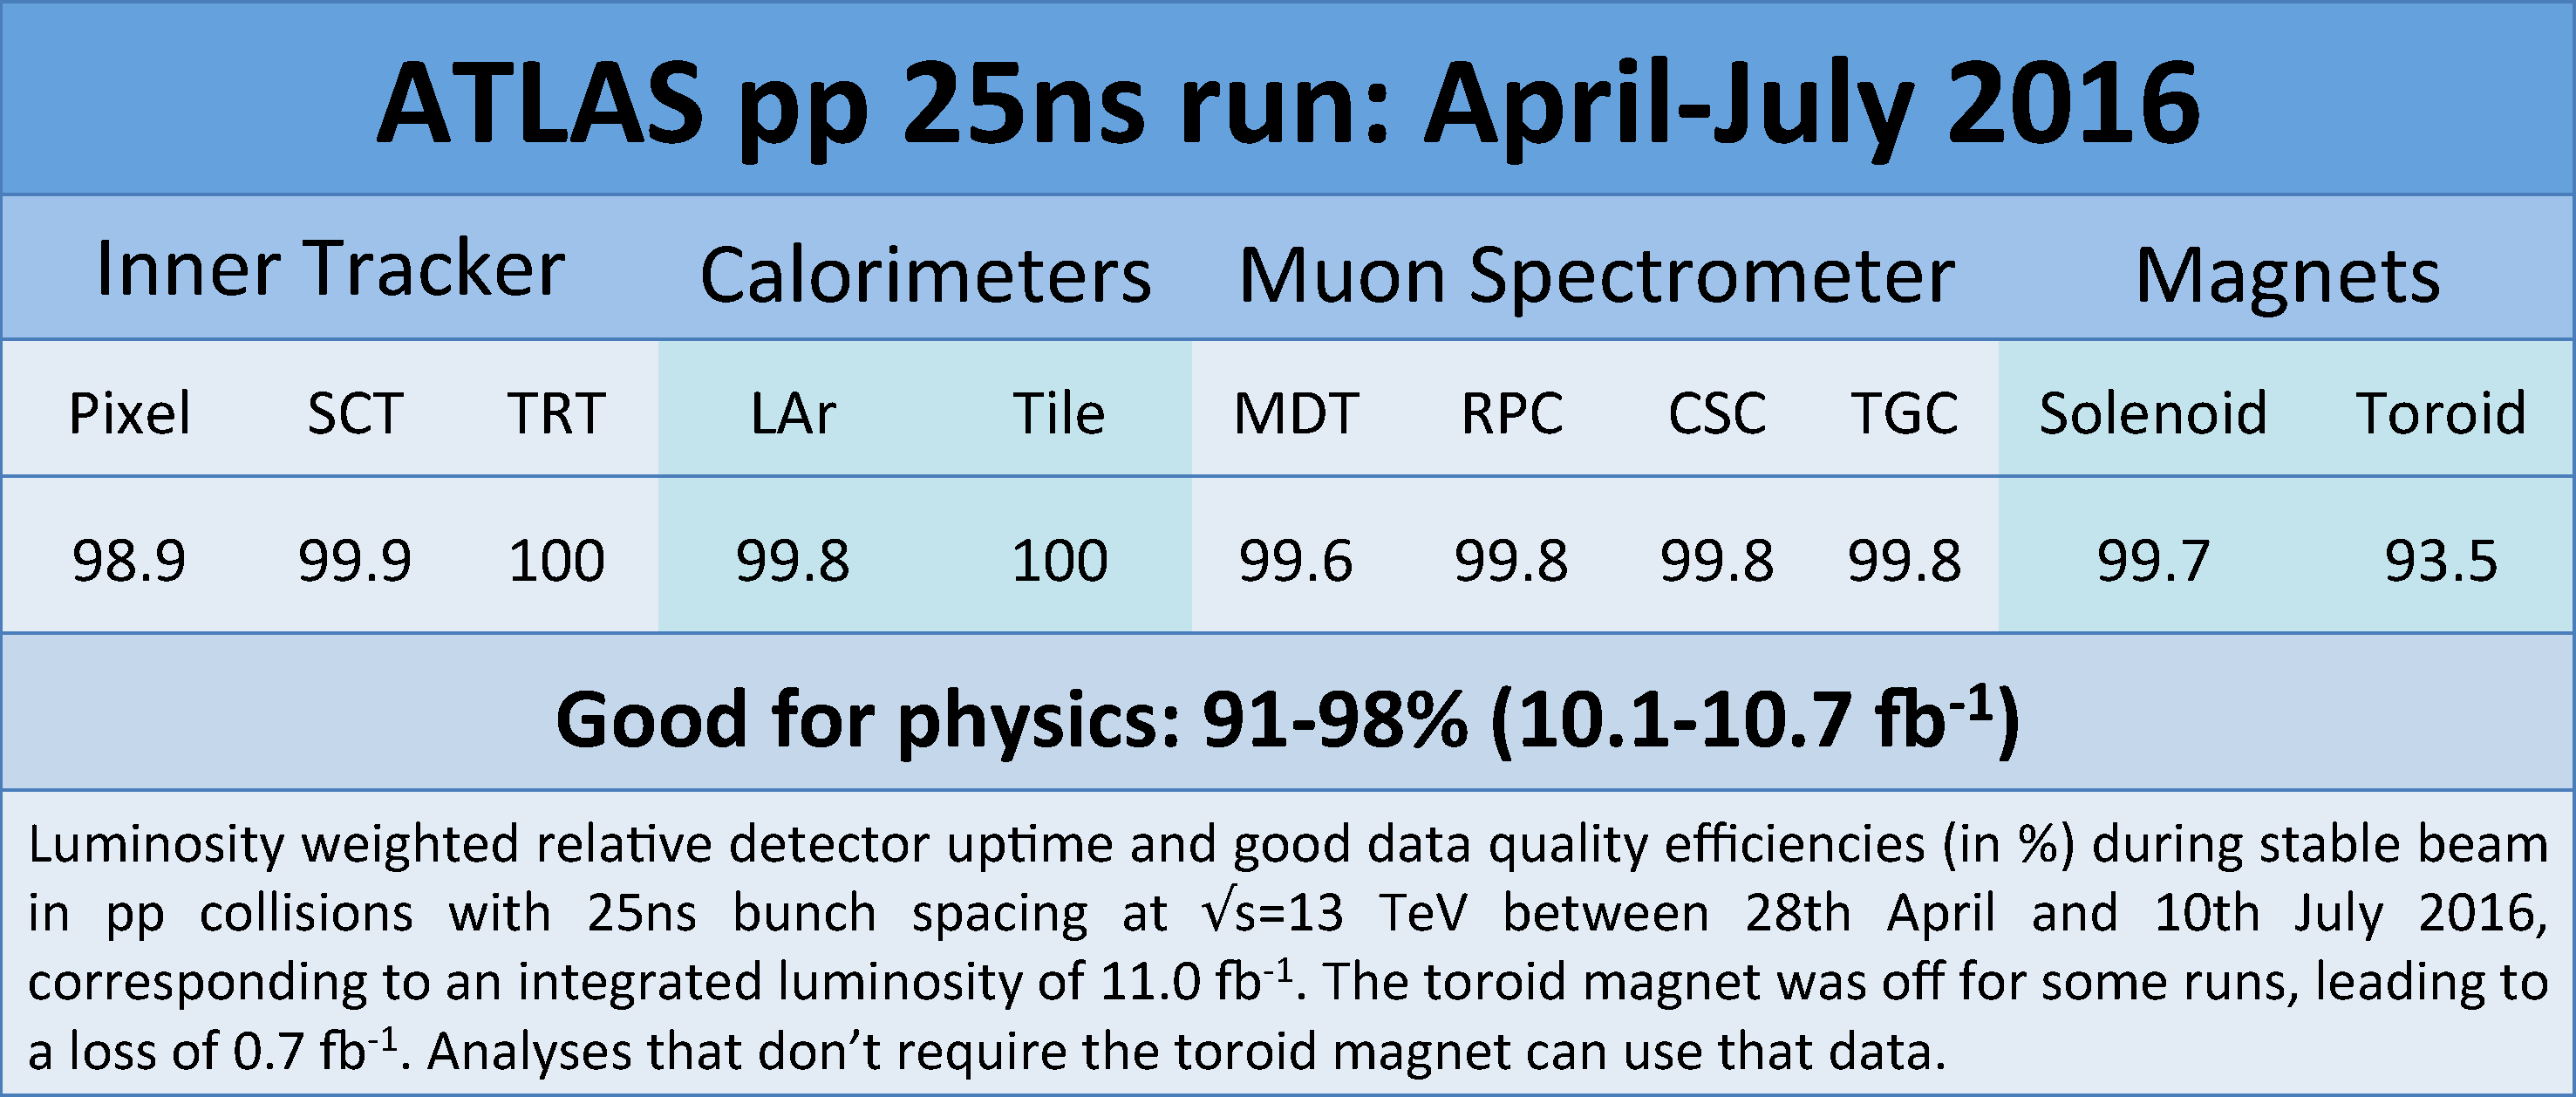
\includegraphics[width=0.85\textwidth]{figures/Detector/DQ2016.png}
\captionsetup{width=0.85\textwidth} \caption{\small Fraction of good data delivered by each subdetector during the year 2015 (top) and 2016 (bottom).}
\label{sec:det:fig:ATLASDQ}
\efig



\begin{table}
\begin{center}
\begin{tabular}{c|c|c|c}
  \hline \hline
  year & LHC delivered & ATLAS recorded & ATLAS good quality \\
  \hline
 2015 & 4.2 fb$^{-1}$ & 3.9 fb$^{-1}$ & 3.2 fb$^{-1}$ \\
 2016 & 38.9 fb$^{-1}$ & 35.9 fb$^{-1}$ & 33.2 fb$^{-1}$ \\
  
  \hline\hline

\end{tabular}
\captionsetup{width=0.85\textwidth} \caption{\small Integrated luminosity per year during Run 2. Columns correspond to LHC delivered luminosity, luminosity recorded by ATLAS, and luminosity with good data quality flag from all subdetectors.}
\label{sec:det:tab:atlum}
\end{center}
\end{table}



\subsection{Future ATLAS upgrades}

In the next years, the LHC will undergo a  series  of  upgrades  leading  ultimately  to  a five-fold  increase  of  the  instantaneous  luminosity  with  leveling according to the High-Luminosity LHC (HL-LHC) project \cite{BejarAlonso:2069130}.  The goal is to extend the dataset from about 300 fb$^{-1}$, expected to be collected by the end of the LHC run (in 2022), to 3000 fb$^{-1}$ by 2035. The foreseen higher  luminosity  at  the  HL-LHC  represents  a  great  challenge  for  ATLAS.\par
A  second  shutdown  (LS2)  is  being  planned  in  2018  to  integrate  the  Linac4  into  the  injector  complex,  to increase the energy of the PS Booster, to reduce the beam emittance, and to upgrade the collider collimation system.  When data taking resumes in 2020, the peak luminosity is expected to reach $\sim 2-3 \times 10^{34}$ cm$^{-2}$s$^{-1}$, corresponding  to  55  to  80  interactions  per  crossing  with  25  ns  bunch  spacing,  well  beyond  the initial  design  goals.
Therefore, to  face the increased event rates, ATLAS will undergo to several upgrades during this long shutdown, referred to as Phase-I upgrade:
\bi
\ib A  replacement  of  the   first  endcap  station  of the  MS,  the  New  Small  Wheel  (NSW) \cite{NSW},  is  proposed.   The  NSW  must  ensure  efficient tracking at high particle rate (up to $5 \times 10^{30}$ cm$^{-2}$s$^{-1}$) and larger $|\eta|$, with position resolution of $<100$ $\mu$m. Furthermore, unlike the present layer, the NSW will be integrated into the Level-1 trigger, thus helping in rejecting background by selecting tracks coming from the primary interaction and matched with the most external layers of the muon spectrometer.
\ib The calorimeter trigger \cite{CALORUP} will also have a an upgrade in Phase I, with the goal of providing higher-granularity,  higher-resolution and longitudinal shower information from the calorimeter to the Level-1 trigger processors.
\ib The Fast TracKer (FTK) \cite{FTK} Trigger will perform the track  finding and  fitting on-line using dedicated massive parallel processing.  FTK will then provide the track parameters with resolution close to that of offline tracks shortly after the start of the Level-2 processing, thus releasing extra resources for more advanced selection algorithms, which ultimately could improve the performance of tracking-based  filter algorithms such as $b$-tagging and $\tau$ identification. While the full geometrical coverage for full Phase-I pileup in foreseen after the 2018 shutdown, a progressive coverage and commissioning already started in 2015.\\
\ei
\noindent The  Phase-I  upgrades  are  designed  to  be  fully  forward-compatible  with  the  physics  programme  of  the  high luminosity HL-LHC (Phase II), when the instantaneous luminosity should reach $\sim 5-7 \times 10^{34}$ cm$^{-2}$ s$^{-1}$, giving 200 interactions per crossing and a total integrated luminosity of 3000 fb$^{-1}$.\par
A third 36-months long shutdown (LS3) in 2023-25 will be necessary to upgrade the accelerator to this ultimate operation mode. ATLAS is being planning major updates in all its subsystems and trigger architecture. The present ATLAS Inner tracker will have several limitations in Phase II, when up to 200 pileup events per bunch crossing are expected.  The entire Inner Detector will be replaced with a new, all-silicon Inner Tracker (ITk) \cite{ITK} with pixel sensors at the inner radii surrounded by microstrip sensors.  A new trigger architecture is being developed that is compatible with the constraints imposed by the detector and provides a  flexible trigger with the potential to deliver the required performance. As currently envisaged, the baseline design for the Phase-II Trigger foresees a split Level-0/Level-1 hardware trigger with a total L1 accept rate of 200 kHz and total latency of 20 $\mu s$.







	
	\chapter{Event simulation}
\label{chp:evtsim}

\begin{flushright}

\begin{small}
\emph{
Nature isn't classical, dammit, and if you want\\ 
to make a simulation of nature, you'd better make it quantum mechanical,\\ 
and by golly it's a wonderful problem, because it doesn't look so easy.\\}
Richard Feynman
\end{small}
\end{flushright}

\minitoc


\label{chp:evtsim:intro}

A key point to test the SM or any possible extension of it is to quantify the consistency of the observed data with the theoretical prediction. 
An accurate simulation, including  the state-of-the-art understanding of the \emph{pp} collision physics and the experimental setup, is necessary to model physics processes and kinematic distributions.
Event simulation is a complex procedure divided into two major steps:
\bi
\ib Event generation: Simulation of the physics process of interest including the modelling of the partonic structure of the incoming protons, their collision and the subsequent event development up to the decays into stable particles. As the physics processes occurring in $pp$ collisions are probabilistic in nature, event generation involves pseudo-random numbers, which are generated using Monte Carlo (MC) techniques.
\ib Detector simulation and digitisation: MC techniques are used to simulate the geometry of the detector, the interaction of particles with the detector materials, and the corresponding detector response, including the digitisation of the detector electronics.
\ei

This chapter presents an overview of the simulation of $pp$ collisions, followed by a description of the MC generators used for the analyses in this dissertation, and the ATLAS detector simulation. It also includes a summary of the procedure followed in ATLAS to validate MC samples, which the author has participated in.\\

\section{Event generation}
\label{chp:evtsim:evtgen}

The modelling of a $pp$ collision requires a detailed understanding of the dynamics of a deep-inelastic interaction at high energy (perturbative QCD), as well as the structure of a relativistic proton and the evolution of partons into stable hadrons at very low energy (non-perturbative QCD). The complication of collisions involving protons is that protons are composite particles, thus a precise understanding of the partonic structure of the proton is needed to calculate the process cross section. A proton is a bound state composed of point-like quarks and gluons interacting among themselves via the constant exchange of soft virtual gluons. According to the uncertainty principle, the time scale of a virtual gluon interaction is inversely proportional to its virtuality $q$, i.e. t $\sim1/q$, so that gluons with higher virtuality usually are absorbed by the same quark by which they were radiated. A hard probe interacts within a much shorter timescale $1/Q \ll 1/q$ during which the partonic fluctuations in the struck proton appear almost frozen. The hard probe effectively takes a snapshot of the proton structure, at a characteristic resolution given by $\sim1/Q$. The independence of long-wavelength (soft) structure on the nature of the hard (short-distance) process, a key aspect in the simulation of $pp$ collision, gives the possibility of factorizing the different processes happening at different energy scales (factorisation theorem).
Since the interaction cross section of such collisions decreases as the momentum exchange $Q$ between the colliding particles increases, a $pp$ collision typically consists of one so-called hard scattering/process with a high momentum exchange $Q$ computed at a fixed order (e.g. next-to-leading order, NLO) in perturbation theory, which is sometimes accompanied by further soft collisions, so-called multi-parton interactions that are instead described via phenomenological models.

\bfig[h!]
\centering
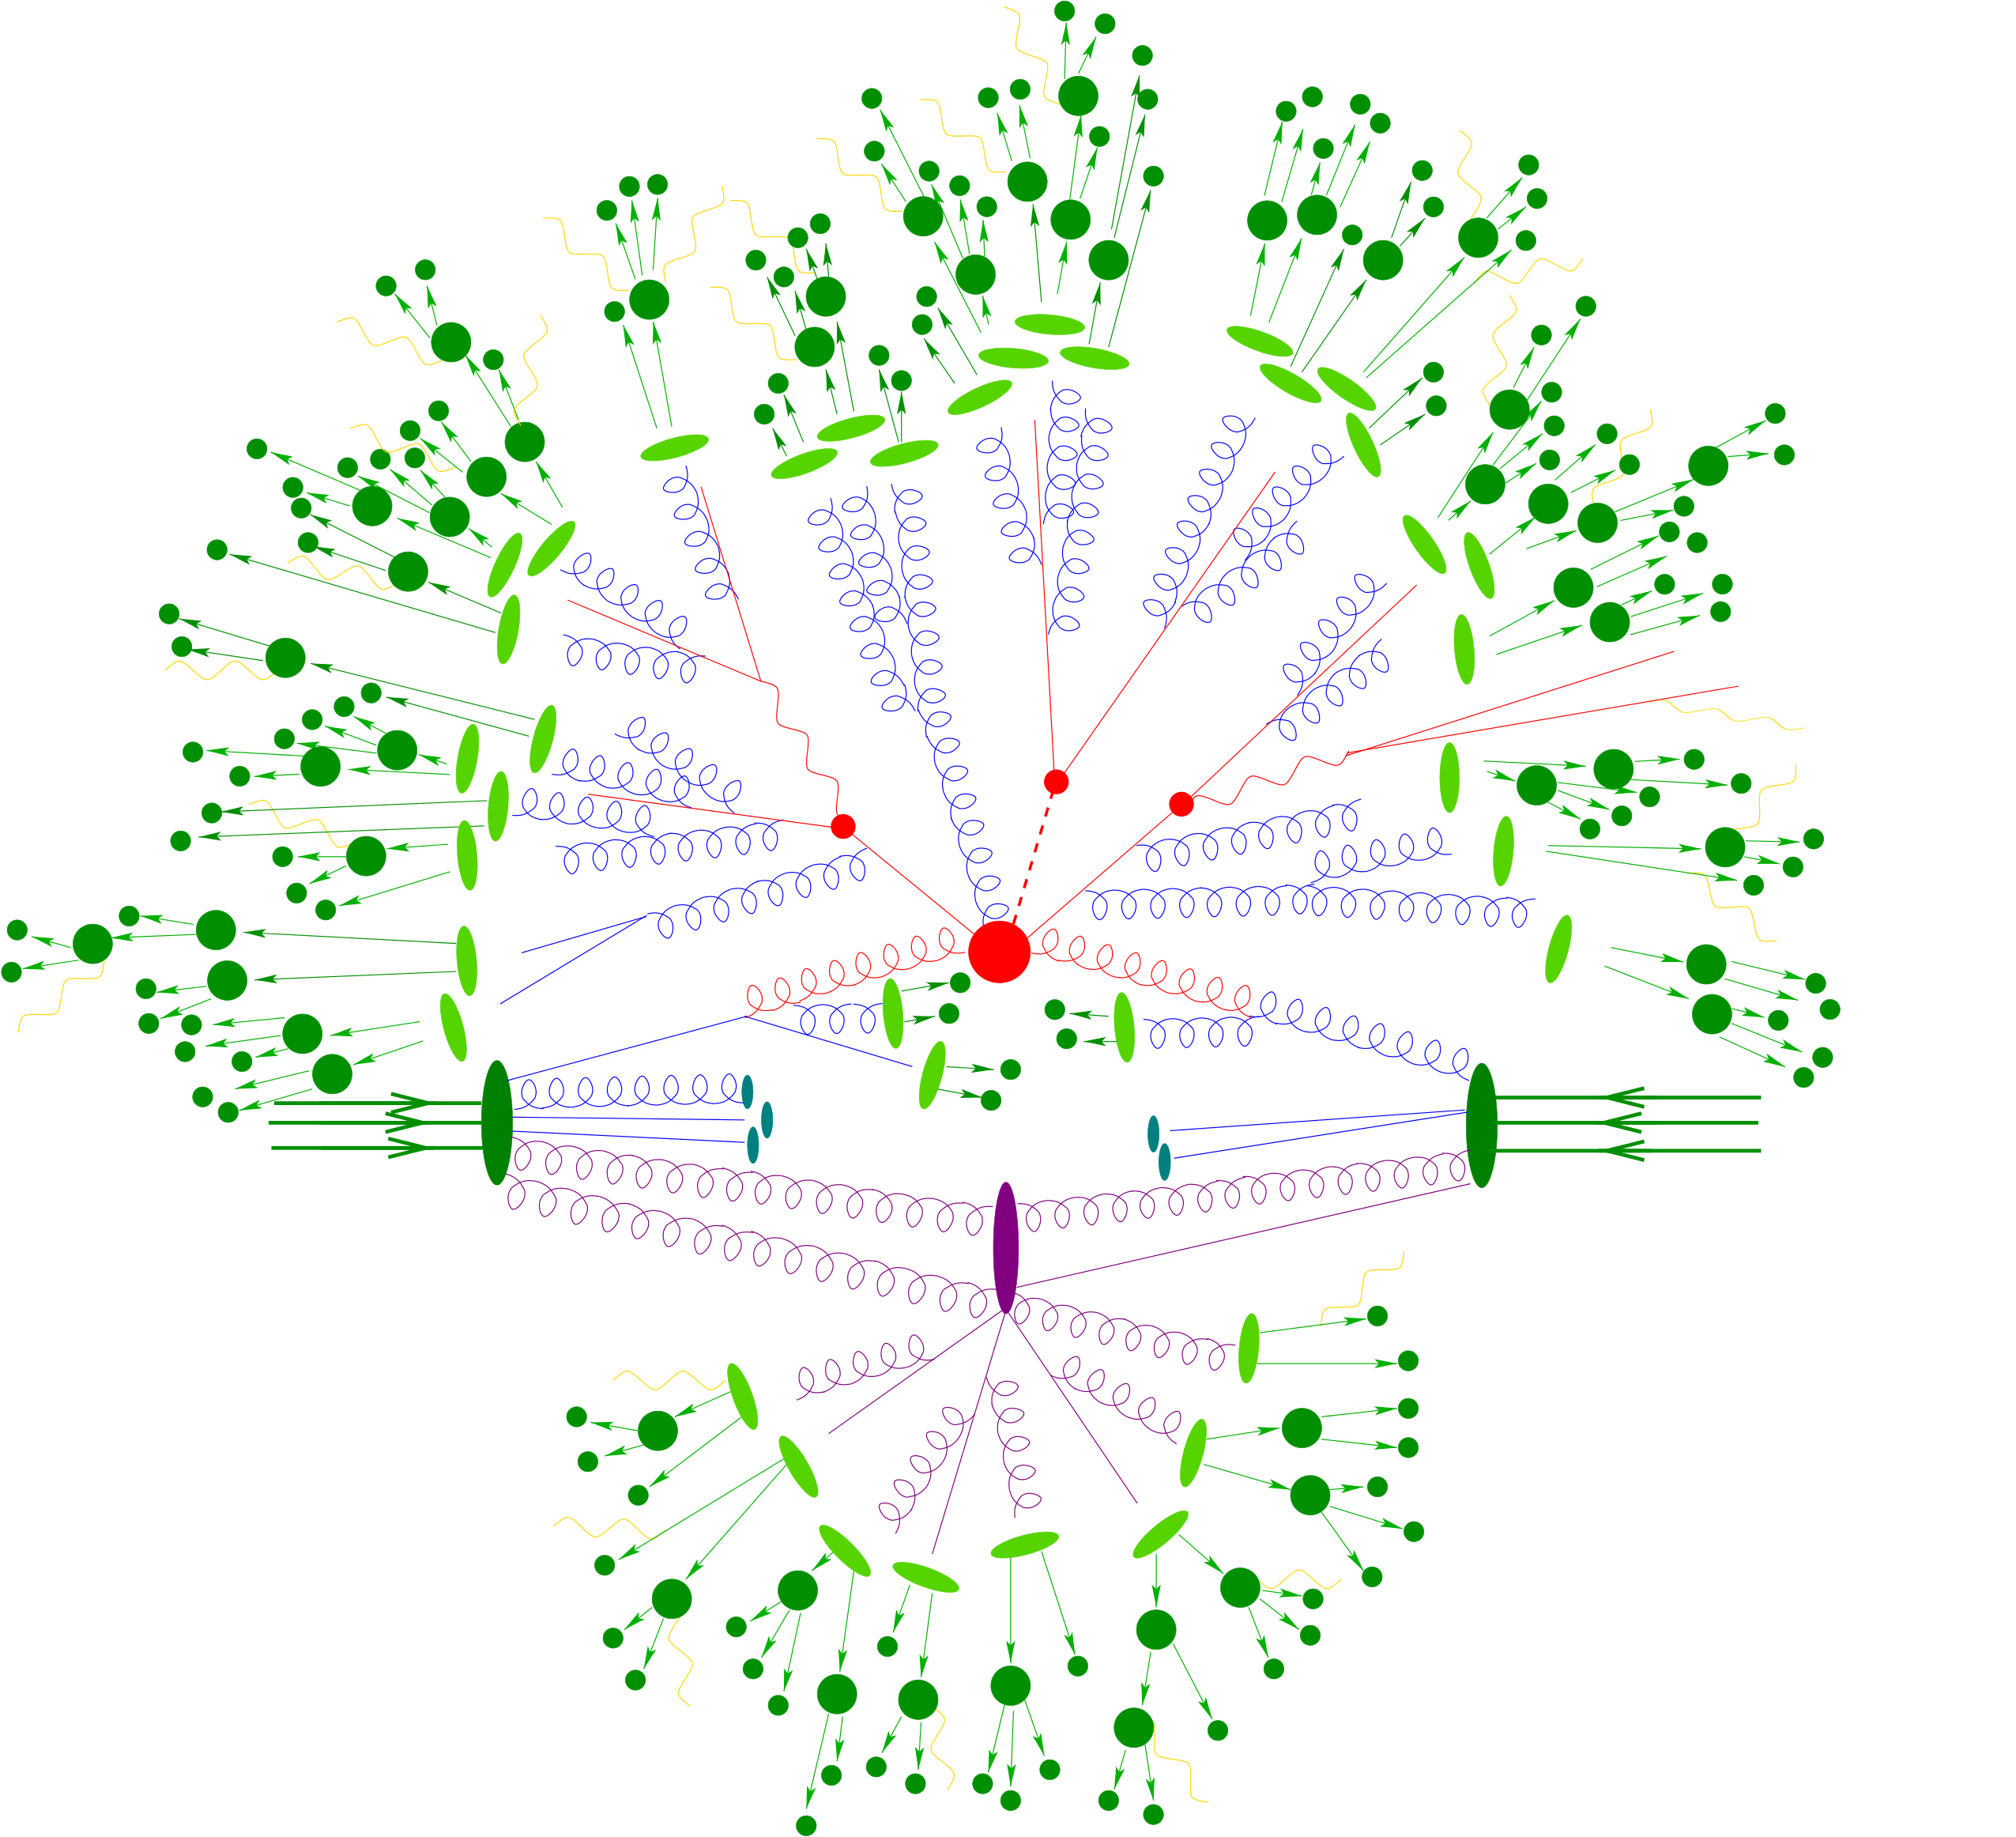
\includegraphics[width=0.8\textwidth]{figures/EvtGen/event}
\captionsetup{width=0.85\textwidth} \caption{\small Illustration of a $pp$ collision. Two partons from the incoming protons (large green ellipses) undergo initial state radiation and interact in the hard process (big red blob). A parton shower (red) emerges from the products of the hard interaction. The resulting partons hadronise into colourless states (light green blobs) that subsequently decay into stable particles (green circles). A secondary interaction between proton remnants is shown as a purple blob, again creating a parton shower (purple), which hadronises, followed by decays into stable particles. This is part of the underlying event, together with the beam remnants (light blue blobs). Electromagnetic radiation (yellow) can be emitted by charged particles at any stage. From reference \cite{Siegert:2010cru}.}
\label{sec:evtgen:fig:evt}
\efig

\subsection{Factorisation theorem}
\label{chp:evtsim:evtgen:hp}

The event simulation begins with the collision, with large momentum transfer, between two partons within the protons. At high energy, the partons behave as asymptotically free, and a perturbative description is applied. The cross section for a generic process $pp \to X$ is defined in terms of the cross section for the partonic processes, according to the factorisation theorem \cite{Collins:1989gx}, as

\be
\sigma_{pp \to X}= \displaystyle\sum_{a,b} \int dx_{a}dx_{b} f_{a}(x_{a},\mu_{F}^{2}) f_{b}(x_{b},\mu_{F}^{2}) \hat{\sigma}_{ab\to X}(x_{a}p_{a},x_{b}p_{b},\mu_{R}^{2},\mu_{F}^{2}),
\ee

\noindent where the sum runs over all possible combinations of the partons $a$ and $b$ able to produce $X$. The parton density function (PDF), $f_{i}(x_{i},\mu_{F}^{2})$, represents the effective density of partons of type/flavor $i$, as a function of the momentum fraction $x_{i}$, when a hadron is probed at a scale $\mu_{F}$. The factorisation scale $\mu_{F}$ represents the estimated limit between the perturbative and non-perturbative QCD regimes, i.e. the energy at which the running $\alpha_{s}$ becomes too large for achieving a desired convergence of the perturbation series. In addition, the cross section calculation depends on the choice of the renormalisation scale $\mu_{R}$ of QCD, at which $\alpha_{s}$ is evaluated. As the factorisation and renormalisation scales describe the not precisely known boundaries between two physics domains, their values are usually related to some quantities characteristic of the modelled process (e.g. the mass of the particle produced, or the sum of the momenta of outgoing particles). The uncertainties arising from such a convention are typically estimated by comparing the cross section values $\sigma_{pp\to X}$ evaluated varying the nominal scale choice for $\mu_{F}$ or $\mu_{R}$ by a factor of two up and down. The cross section for the partonic process $\hat{\sigma}_{ab\to X}(x_{a}p_{a},x_{b}p_{b},\mu_{R}^{2},\mu_{F}^{2})$  is computed explicitly at a fixed order in perturbation theory. This step is also referred to as Matrix Element (ME) calculation, because it involves the calculation of the scattering matrix relating the initial and final state particles of the process.

\bfig[h!]
\centering
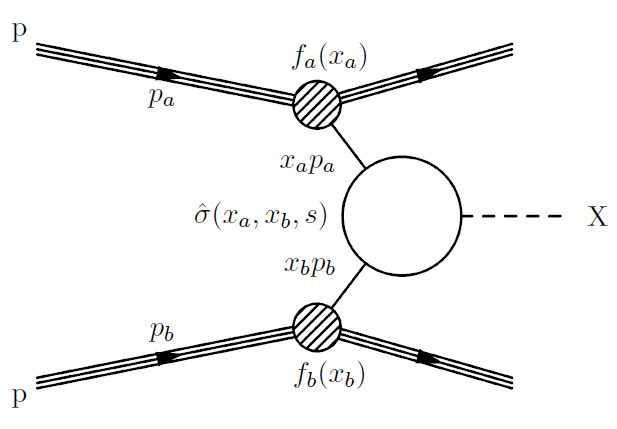
\includegraphics[width=0.6\textwidth]{figures/EvtGen/hs.png}
\captionsetup{width=0.85\textwidth} \caption{\small Illustration of a hard scattering. A parton with four-momentum $x_{a}p_{a}$, originating from a proton with a four-momentum $p_{a}$, undergoes a hard collision with a parton carrying a four-momentum  $x_{b}p_{b}$, coming from a proton with a four-momentum $p_{b}$. The spectator partons do not influence the hard interaction and continue their trajectory with slightly distorted directions.
}
\label{sec:evtgen:fig:hs}
\efig


\subsection{Parton density functions}
\label{chp:evtsim:evtgen:pdf}
QCD does not predict the structure of the proton and therefore the PDFs cannot be calculated, but have to be measured from experimental data. Historically, most of the information came from Deep-Inelastic Scattering (DIS) in fixed-target lepton-nucleon scattering experiments and from the HERA electron-proton collider at DESY. The energy dependence of the PDFs is given by the DGLAP evolution equations \cite{DGLAP1,DGLAP2,DGLAP3}:


\begin{equation}
\frac{\partial q_{i}(x,Q^{2})}{\partial \log Q^{2}}=\frac{\alpha_{s}}{2\pi} \int_x^1 \frac{dz}{z} \left \{ P_{q_{i}q_{j}}(z,\alpha_{s})q_{j}(\frac{x}{z},Q^{2}) + P_{q_{i}g}(z,\alpha_{s})g(\frac{x}{z},Q^{2})\right\},
\end{equation}
\begin{equation}
\frac{\partial g(x,Q^{2})}{\partial \log Q^{2}}=\frac{\alpha_{s}}{2\pi} \int_x^1 \frac{dz}{z} \left \{ P_{gq_{j}}(z,\alpha_{s})q_{j}(\frac{x}{z},Q^{2}) + P_{gg}(z,\alpha_{s})g(\frac{x}{z},Q^{2})\right\}.
\end{equation}

In the above expressions, $g(x,Q^{2})$ is the gluon PDF, $q_{i}(x,Q2)$ is the quark PDF, and $P_{ab}(z, Q^{2})$ are the splitting functions. 
For the evolution in $x$, there are no such equations, but it has to be obtained from fits to experimental data. Several collaborations continuously work to improve the PDF fits with the most recent data. PDF sets  from the groups CTEQ \cite{ct10}, NNPDF \cite{Ball:2012cx} and MSTW \cite{mstw1} are extensively used at the LHC.

\bfig[h!]
\centering
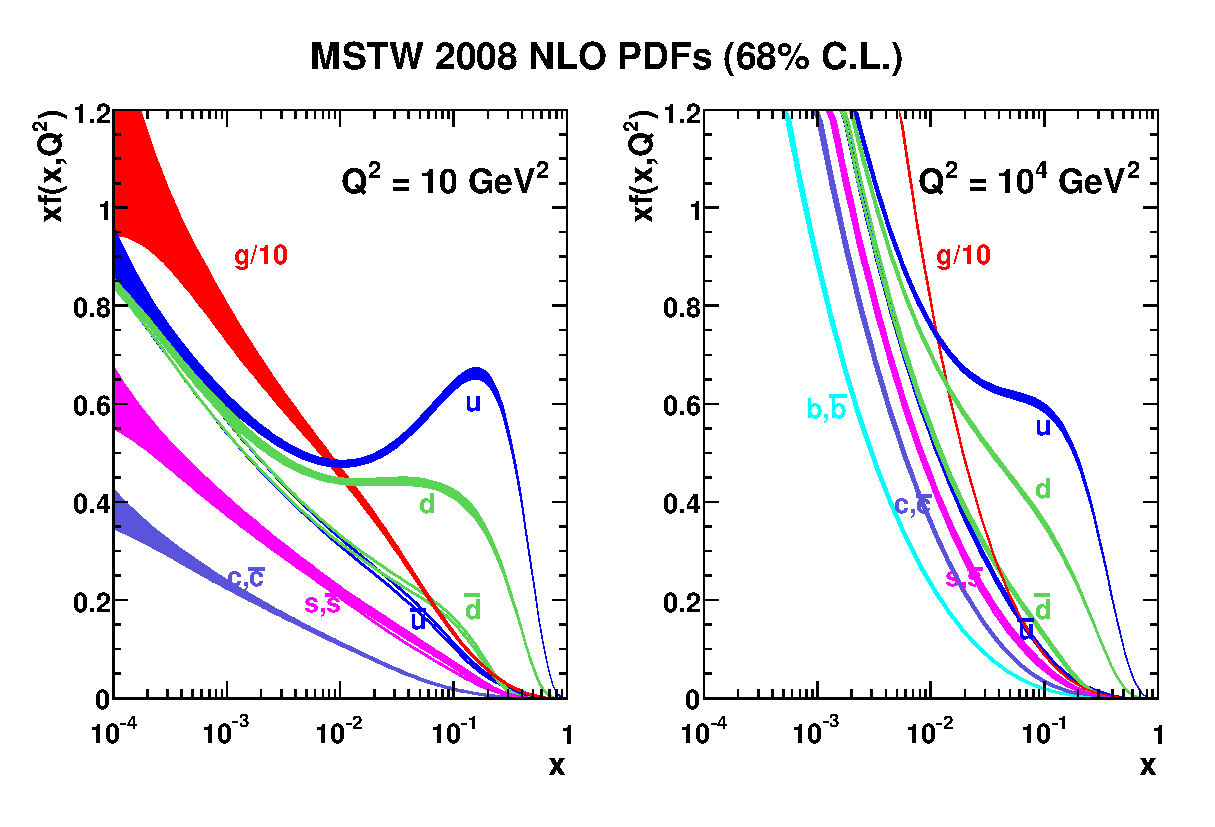
\includegraphics[width=0.7\textwidth]{figures/EvtGen/PDFplot.eps}
\captionsetup{width=0.85\textwidth} \caption{\small Parton luminosities for MSTW 2008 NLO PDF set as function of $x$ with the uncertainty band. On the left (right) panel for $Q^{2}=10$ $(10^{4})$ $\gev^{2}$. From reference \cite{mstw1}.}
\label{sec:evtgen:fig:pdf}
\efig


\subsection{Matrix element}

The production of an arbitrary final state, $ab \to X$, from a hadron collision can be expressed to all-orders in perturbation theory as:

\be
\hat{\sigma}_{ab\to X}= \underbrace{\displaystyle\sum_{k=0}^{\infty}\int d\Phi_{X+k}}_{\sum \rm legs}\underbrace{|\displaystyle\sum_{\ell=0}^{\infty}\mathcal{M}_{X+k}^{(\ell)}|^{2}}_{\sum \rm loops},
\ee

\noindent where $\mathcal{M}_{X+k}^{(\ell)}$ is the amplitude for producing $X$ in association with $k$ additional final-state partons (real emission corrections, or ``legs'')  and with $\ell$ additional virtual correction loops. The phase space of the configuration with $k$ legs is represented by $d\Phi_{X+k}$.  Specific values of $k+\ell$ will return the fixed-order calculations of perturbative QCD:
\bi
\ib $k=0$, $\ell=0$ $\implies$ LO (usually tree-level) for $X$ production;
\ib $k=n$, $\ell=0$ $\implies$ LO for $X$+$n$ jets;
\ib $k+\ell$ $\le$ n $\implies$ $N^{n}$LO for $X$ (includes $N^{n-1}$LO for $X$+1 jet, $N^{n-2}$LO for $X$+2 jets, and so on up to LO for $X+n$ jets ).
\ei


According to the KLN theorem \cite{KLN1,KLN2}, the infrared (IR) singularities coming from integrating over collinear and soft real-emission configurations should cancel, order by order, with those coming from the IR-divergent loop integrals.
However, in a fixed-order calculation, e.g. leading order, in the situation for which $k\ge1$, $\ell=0$, the integration over the full momentum phase space will include configurations in which one or more of the $k$ partons become collinear or soft. Such configurations leads to IR singularities in the integration region, which must be regulated cutting away the problematic regions of the phase space. The remaining part of the phase space is then considered by parton-shower generators.


\subsection{Parton shower}

Partons involved in a hard-scatter process normally have a very high energy ($Q>1$ $\gev$) for which $\alpha_{s}$ is small ($\ll$1). At such energies, quarks and gluons are likely to radiate off a gluon, carrying a portion of the energy of its mother particle and a colour connection to it. These gluons can then decay into further gluons or quark-antiquark pairs, leading to the formation of parton showers. This process continues as long as the particles produced have sufficient energy ($Q>1$ $\gev$) to reach a distance from the initial particle at which the colour field breaks up into a quark-antiquark pair.
Parton Showers (PS) populate regions of the phase space where emissions are collinear or soft (IR divergent) providing an all-orders resummation using an approximation scheme with a leading-logarithmic (``leading-log'') accuracy. The parton shower contribution to the hard process cross section is thus estimated by including only the dominant contribution to each order.
Starting from a differential cross section for $n$ particles $d\sigma_{n}$, a differential cross section for $n+1$ particles is calculated parametrising the probability that the new particle $j$ carries a fraction $z$ of the energy of its mother particle $i$ emitted at a virtuality scale or invariant mass $q^2$ using the splitting function $P_{ij}(z,q^{2})$:

\be
d\sigma_{n+1}\approx d\sigma_{n}\frac{\alpha_{s}}{2\pi}\frac{dq^{2}}{q^{2}}dz P_{ij}(z,q^{2}).
\label{eq:evtsim:evtgen:nplusone}
\ee

The simulation algorithm develops the shower by applying equation \ref{eq:evtsim:evtgen:nplusone} iteratively, for each parton involved in the hard interaction. The splitting functions obviously play a crucial role driving the emission probabilities. In MC simulations the formulation of parton shower uses a more convenient expression using the so-called Sudakov form factors:

\be
\Delta_{i}(q_{1}^{2},q_{2}^{2})=\exp\left( - \displaystyle\sum_{j \in q,g } \int_{q_{2}^{2}}^{q_{1}^{2}} \frac{dq^{2}}{q^{2}} \int_{z_{\rm min}}^{z_{\rm max}} \frac{\alpha_{s}}{4\pi} dz P_{ij}(z,q^{2})\right),
\label{eq:evtsim:evtgen:sudakov}
\ee

\noindent which represent the unconditional survival probability for a parton not to undergo a resolvable emission process between the two energy scales $q_{1}^{2}$ and $q_{2}^{2}$. The algorithm implemented in MC simulations goes through the following steps:
\bi
\ib Given the initial scale $Q^2$, referred to as resummation scale, it produces an emission at scale $q_{2}^{2}$ using equation \ref {eq:evtsim:evtgen:sudakov}.
\ib If the value of $q_{2}^{2}$ is lower than the hadronisation scale, $q_{2}^{2} \ll Q_{0}^{2} \approx 1$ $\gev^{2}$ no further emission occurs, thus the shower developments stops and hadronisation takes place.
\ib Otherwise, further emissions will occur and the process is repeated for each new parton using $q_{2}^{2}$ as initial scale.
\ei


Final-state radiation (FSR), i.e. a gluon radiated off a final-state parton is generated through the above parton shower procedure. For the initial-state radiation (ISR), however, this procedure is not suitable, as the momenta of the partons initiating the hard process need to be precisely adjusted to produce the hard process (e.g. a gluon decaying into a $t\bar{t}$ pair). Thus, the longitudinal momentum fractions $x_{1}$ and $x_{2}$ of the incoming partons need to be simulated first, and the momentum and angle of the ISR is found by backwards evolution, which involves a PDF-dependent correction to the Sudakov form factors. Due to the existing colour connections, the direction of the ISR tends to be aligned with that of mother parton.

\subsection{Matrix element and parton shower matching}

To improve the leading-log (LL) description given by the parton shower, it is often necessary to go beyond the approximations made in that step. One possibility is to replace the parton-shower approximation at given orders in the strong coupling expansion by exact perturbative QCD results. The left panel of the figure \ref{sec:evtgen:fig:dc} describes the LO cross section computation for some process $X$ and interfacing the parton shower to it.
\bfig[t!]
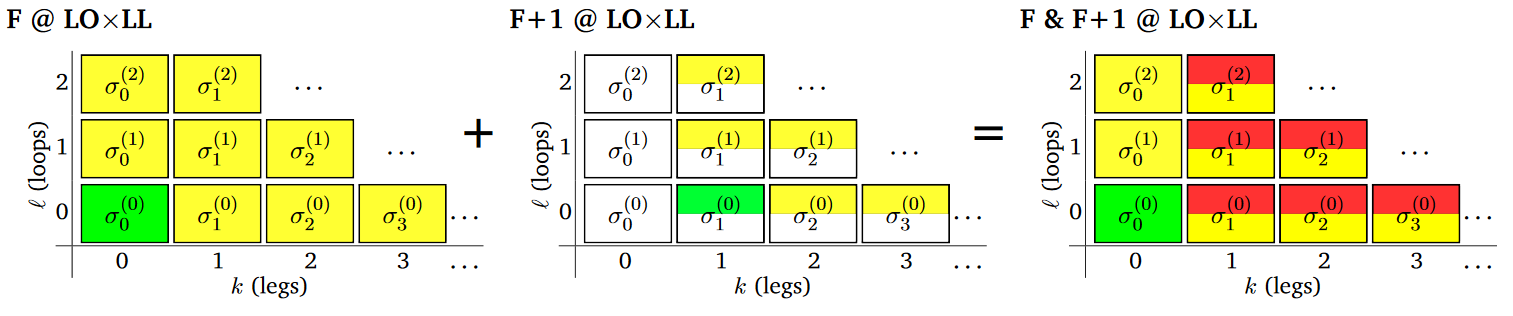
\includegraphics[width=\textwidth]{figures/EvtGen/doublecounting.png}
\captionsetup{width=0.85\textwidth} \caption{\small The double-counting problem caused by adding cross sections involving matrix elements with different numbers of legs when interfaced to parton showers. From reference \cite{Skands:2012ts}.}
\label{sec:evtgen:fig:dc}
\efig
This only gives a LL description of $X+1$ parton. To improve this precision LO matrix element for $X+1$ parton is added with an infrared cut-off to prevent divergences from soft and collinear emissions (see central panel of the figure \ref{sec:evtgen:fig:dc}).  By doing so, final states with one additional emission are generated as both the matrix-element term for $X + 1$ parton, and in the first radiation of the parton shower starting from the $X + 0$ parton.  Furthermore, final states with more than one parton are generated twice by the parton shower (see right panel of the figure \ref{sec:evtgen:fig:dc}). This
double-counting problem becomes worse as matrix elements with more legs are added. The double-counting problem can be avoided by separating the phase space to be covered by the parton shower and the matrix element (ME-PS matching). However, such a separation may produce discontinuities in observable spectra because the matrix element includes non-divergent components that are ignored in the parton shower. These procedures are based on the matching of the coefficients calculated by the two parts of the full calculation, parton showers and matrix elements, for each order in perturbation theory, so that the nesting of inclusive and exclusive cross sections is respected without double counting. The  parton-shower  expression  at  fixed  order  is  computed  and  subtracted  from  the  higher-order calculation to remove double counting.  The subtracted result is processed by the parton shower.\par
These merging schemes typically separate the phase space for emissions into hard and soft/collinear regions by means of a jet criterion, and use the parton shower to fill soft/collinear emissions while using the fixed-order calculation to provide hard/large-angle emissions. Several solutions to this problem have been proposed and implemented in event generators: the CKKW method \cite{Catani:2001cc}, the MLM prescription \cite{Mangano:2006rw}, and the POWHEG method \cite{powbox1}. Among them, multi-jet ($\ge2$ jets) matrix elements can be included by the CKKW method and the MLM prescription only, both based on the suppression method in which multijet events coming from matrix elements are suppressed by reinterpreting them in the picture of a parton shower. Generalisations of the CKKW and MLM methods to perform merging of multileg NLO matrix elements with parton shower are available at NLO; the MLM prescription is known at NLO as the FxFx method \cite{Frederix:2012ps}.\\
The CKKW algorithm is as follows:
\bi
\ib Construct a shower history by applying the $k_{\rm T}$ algorithm to the state from the matrix element.
\ib Reweight the event with the product of the Sudakov form factors calculated for each branching and the running coupling weight calculated in each branching vertex.
\ib Set the starting scale of each parton to the scale associated with the node in the shower history where it was produced. Invoke the shower and veto any emission which would give a $k_{\rm T}$ measure above a certain threshold.
\ei

\noindent The MLM algorithm proceeds through the following steps:
\bi
\ib Select a merging scale $Q_{\rm MS}$ and a matrix element cutoff $Q_{\rm cut}$ such that $Q_{\rm cut}<Q_{\rm MS}$, where the scales are defined using a jet algorithm.
\ib Cluster the partons from the matrix element using the $k_{T}$ algorithm and use the clustering scales as in input to $\alpha_s$ and reweight the event.
\ib Cluster the partons to jets using the algorithm from the first step with a clustering scale set to $Q_{\rm MS}$. Go through the list of partons, in order of decreasing energy, and match them to the clustered jets. This is done by finding the jet with the smallest distance to the parton defined using some measure based on the jet clustering scheme. If not all partons match or there are extra jets, reject the event.
\ei



\subsection{Hadronisation}

The development of the parton shower stops when the partons generated have a virtuality below the hadronisation scale, a regime in which  the strong coupling constant $\alpha_{s}$ becomes large and causes their confinement into colourless hadrons. This process is known as hadronisation. It occurs in the non-perturbative regime of QCD and thus relies on phenomenological models. The most widely used hadronisation models are the Lund String Model \cite{Andersson:1983ia,Sjostrand:1984ic} and the Cluster Model \cite{Webber:1983if,Marchesini:1987cf}.\par
The Lund String Model is based on the observation that the quark-antiquark  potential  rises  linearly  with  the  distance  between  quarks  in  a  meson  system. It is translated into a narrow flux tube stretched between the two quarks. Thus, this field is described as a string stretching between the quark and
the antiquark. Gluons produced in the parton shower give rise to kinks on the string. When the string energy overcomes the mass threshold of a given quark-antiquark pair, it can break forming an antiquark to match the original quark, and a quark to match the original antiquark, and leaving three shorter strings with lower potential energy. This procedure continues until the energy of the particles drops below the point at which they can no longer escape the confinement. At that point they combine forming the final-state hadrons. This model has some problems describing baryon production. In the simplest scheme for baryon production, diquark pairs are produced instead of quark pairs.  A more advanced model is the popcorn approach, where baryons appear from multiple production of quark pairs. The string model of jet fragmentation is infrared and collinear safe, because a soft or collinear gluon induces a vanishingly small kink on the color string.\par
The Cluster Model is based on the pre-confinement property of QCD. This means that at each point the parton shower forms color-singlet combinations of partons, called clusters, which have an asymptotically universal invariant mass distribution.
Thereby, all remaining gluons in the shower are forced to split into quark-antiquark pairs, which participate in the formation of clusters.
Once  primary  clusters  are  formed,  the  ones  with  mass  below  $3-4$  $\gev$  are  transformed  into  hadrons through a two-body decay according to phase space.  Heavier clusters may  first undergo non-perturbative splitting  processes,  and  decay  into  two  lighter  clusters,  or  a  lighter  cluster  and  a  hadron,  before the cluster-to-hadron transition is resumed.  This process is repeated until all clusters have been transformed into hadrons. However, this model has problems dealing with the decay of very massive clusters, and inadequately suppressing baryon and heavy-quark production.

\begin{figure}[h!]
\begin{subfigure}{0.5\textwidth}
  \centering
  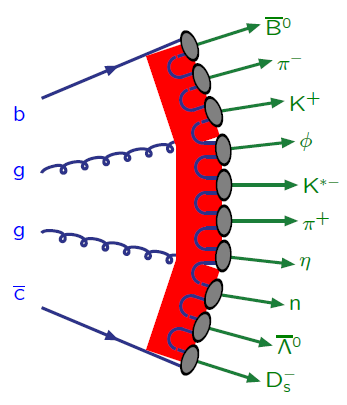
\includegraphics[width=0.6\textwidth]{figures/EvtGen/string.png}
  \captionsetup{width=0.85\textwidth} \caption{}
  \label{sec:evtgen:fig:cluster}
\end{subfigure}
\begin{subfigure}{0.5\textwidth}
  \centering
  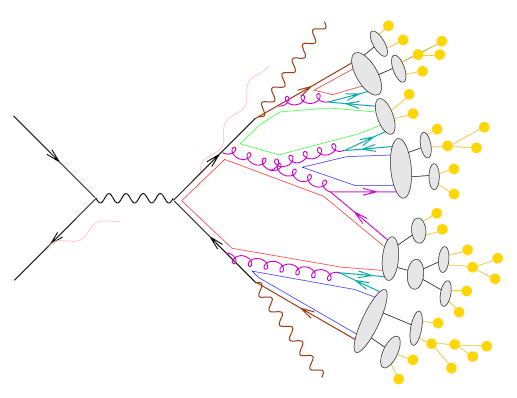
\includegraphics[width=0.9\textwidth]{figures/EvtGen/cluster.png}
  \captionsetup{width=0.85\textwidth} \caption{}
  \label{sec:evtgen:fig:string}
\end{subfigure}

\captionsetup{width=0.85\textwidth} \caption{\small The models of (a) string fragmentation and (b) cluster hadronisation.}
\label{sec:evtgen:fig:hadro}
\end{figure}

\subsection{Underlying event}

The processes discussed so far, i.e. the hard process, its higher-order corrections (parton shower) and development (hadronisation), are initiated by one parton from each incoming proton, neglecting  any effects of rescattering and the exchange of multiple partons between the initial-state protons. However, the event development receives a contribution from additional soft or moderately-hard processes, jointly referred to as ``underlying event'' (UE). The description of the UE employs phenomenological models, because of the non-perturbative nature of the processes involved. The  UE is considered to be composed of thee dominant components: multiparton interactions, beam remnants and pileup.\par
Multiparton interactions (MPI) correspond to moderately-hard interactions of the spectator partons among the incoming protons, i.e. those partons not participating in the hard process. The first detailed MC model for perturbative MPI was proposed in \cite{Sjostrand:1987su}. In this model, the crucial observation is that the t-channel propagators go on shell at low $p_{\bot}$, causing the differential cross sections to become very large. At the LHC  this parton-parton cross section becomes larger than the total hadron-hadron cross section at $p_{\bot}$ scales of order $4-5$ \gev (see figure \ref{sec:evtgen:fig:mpi}). In the context of MPI models, this is interpreted to mean that each hadron-hadron collision contains several few-$\gev$ parton-parton collisions. MPI interaction typically results in a pair of low-$\pt$ back-to-back jets that are colour connected with the rest of the event.

\bfig[h!]
\centering
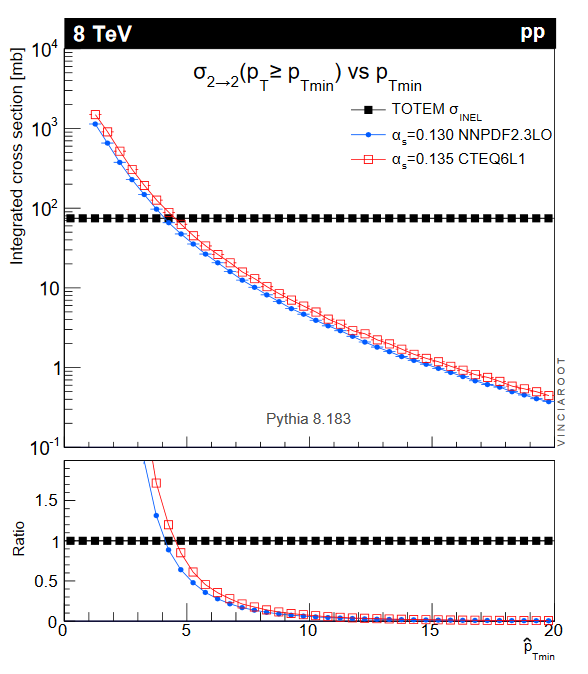
\includegraphics[width=0.5\textwidth]{figures/EvtGen/mpi.png}
\captionsetup{width=0.85\textwidth} \caption{\small Comparison of the total inelastic proton-proton cross section at $\sqrt{s}=8$ $\tev$ as measured by TOTEM, with the parton-parton cross section at LO in QCD as a function of the minimum parton $p_T$ ($\hat{p}_{{\rm T}{\rm min}}$). The fact that the curves cross at a scale of $\sim5$ $\gev$ is interpreted to mean that this is a characteristic scale relevant for MPI. From reference \cite{Skands:2012ts}.}
\label{sec:evtgen:fig:mpi}
\efig

Incoming beam particles may leave beam remnants that have not undergone any inelastic scattering. These remnants represent the soft QCD activity and need to be put together and colour connected with the rest of the event. What is left in the beam remnant is then a number of partons, with flavours given by the remaining valence content plus the number of sea quarks required for overall flavour conservation. Gluons in the remnant are not explicitly accounted for but are implicit as confinement clouds around the quarks.  Beam remnants are modelled by conserving the colour connection and momentum within the event.\par
Pileup, as discussed in section \ref{chp:det:LHC:design}, refers to the presence of additional inelastic $pp$ collisions in the event originating within the same bunch crossing (in-time) or from an event in a different bunch-crossing (out-of-time). Pileup represents a serious challenge to the reconstruction of the hard process as the products of pileup events largely overlap with those of the hard process (although in the case of in-time pileup typically originating from a vertex displaced with respect to that of the hard scattering). In-time pileup consist of soft QCD interactions and are modelled in a similar way as the UE. Out-of-time pileup is modeled with the same physics process, but considering interactions in past bunch crossings and simulating the time response of the readout electronics. In chapter \ref{chp:obj} several techniques to mitigate impact of pileup on reconstructed objects will be discussed.


\subsection{Event generators}

Event generators are tools that simulate collision events and their development, using the MC method. Generators can be either general-purpose, performing all steps in the event development, or specialised for a particular step of the event generation. Commonly used generators differ in the approach to various elements of event generation. While some use only a LO matrix-element calculation, others include higher-order corrections, as well as various parton-shower or hadronisation models. In this section, the general features of the generators used in the studies documented in this dissertation are briefly summarised.

\subsubsection{General-purpose Monte Carlo generators}

\bi
\ib {\sc Pythia} \cite{Sjostrand:2006za,Pythia8} is a MC generator using LO calculations for $2\to n$ $(n\leq3)$ processes, it can simulate collisions at high energies between elementary particles such as $e^{+}$, $e^{-}$, $p$ and $\bar{p}$ in various combinations. It contains theory and models for a number of physics aspects, including hard and soft interactions, parton distributions, initial- and final-state parton showers (emissions ordered in transverse momentum), multiparton interactions, fragmentation (Lund string model) and decay.
\ib {\sc Herwig} \cite{herwigpp} has the same capabilities as {\sc Pythia} with few small differences. It computes $2\to2$ processes using LO matrix elements. The parton-shower approach includes colour-coherence effects, with special emphasis on the correct description of radiation from heavy particles, and features emissions ordered in opening angle. The formation of hadrons from the quarks and gluons produced in the parton shower is described using the cluster hadronisation model. {\sc Herwig} is typically interfaced with the standalone software {\sc Jimmy} \cite{jimmy} that simulates the UE.
\ib {\sc Sherpa} \cite{Gleisberg:2008ta} is a multi-purpose MC generator that can provide multileg NLO/LO calculations (ME-PS matching uses CKKW method both at NLO and LO) It can simulate collisions between $e^{+}$, $e^{-}$, $p$ and $\bar{p}$ in various combinations. It contains theory and models for a number of physics aspects including BSM processes. It contains its own parton shower algorithm based on the Catani-Seymour dipole formalism \cite{Schumann:2007mg} and its own UE modelling. It can be interfaced with {\sc OpenLoops} \cite{Cascioli:2011va} to compute loop amplitudes and {\sc Comix} \cite{Gleisberg:2008fv} to generate matrix element amplitudes. 
\ei

\subsubsection{Matrix Element Monte Carlo generators}
\bi
\ib {\sc Powheg-Box} \cite{powheg} is an NLO parton-level generator using the {\sc Powheg} method  \cite{powbox1}. It generates the hardest radiation in the event using the exact NLO matrix element and is normally interfaced with another parton-shower MC generator (usually {\sc Pythia} or {\sc Herwig}) for showering, hadronisation and UE modelling.
\ib {\sc MadGraph5$\_$aMC@NLO} \cite{Alwall:2014hca} is an automated MC generator of LO/NLO matrix elements. The NLO calculation implements the {\sc MC@NLO} method \cite{mcatnlo_1}. It is normally interfaced with another parton-shower MC generator (usually {\sc Pythia} or {\sc Herwig}) for showering, hadronisation and UE modelling. It can perform ME-PS merging LO using the MLM prescription and at NLO using the FxFx method. It contains theory models and new ones can easily be added using UFO models \cite{Degrande:2011ua}.  
\ib {\sc Protos} \cite{protos}  is a LO ME generator for some BSM processes involving the top quark.  It can be  interfaced with {\sc Pythia} for showering and hadronisation.
\ei

\subsubsection{Specialised Monte Carlo generators}
\bi
\ib {\sc Photos} \cite{PhotosPaper} is a MC generator used to model bremsstrahlung in particles decay. It runs after parton shower ({\sc Pythia} or {\sc Herwig}) on the HepMC event record.
\ib {\sc Tauola} \cite{TauolaPaper}  is MC event generator that simulates tau decays for both leptonic and hadronic  decays  modes. It runs after parton shower ({\sc Pythia} or {\sc Herwig}) on the HepMC event record.
\ib {\sc EvtGen} \cite{Lange:2001uf} is  a MC that implements a detailed description of the physics of $b$-hadrons. In particular, it includes detailed models for semileptonic decays, CP-violating decays, and produces accurate results for angular distributions in sequential decays, including all correlations. It runs after parton shower ({\sc Pythia} or {\sc Herwig}).
\ei




\section{Detector simulation}
\label{chp:evtsim:detsim}


MC generators produce a list of four-vectors of all stable particles produced in the event, after hadronisation and decay of the intermediate unstable particles. This is usually referred to as particle level. In order to compare it with the collider data, the MC events have to be processed through the ATLAS detector simulation to model the interactions of the resulting stable particles with the sensitive and dead material of the detector (reconstruction level). The most significant interactions  with  the  detector are simulated with {\sc Geant4} framework \cite{geant}. The resulting energy deposits are converted into simulated electronic signals taking into account the geometry, detector response and readout system of the ATLAS detector. A faster simulation (AF2) \cite{AFII} was developed to reduce the CPU time necessary to process the event by applying a parameterised description of the particle showers in the calorimeters.
Figure \ref{sec:evtgen:fig:ATLASsim}  shows the ATLAS simulation data flow with the different steps for the MC and data processing.


\bfig[h!]
\includegraphics[width=\textwidth]{figures/EvtGen/atlassimul.png}
\captionsetup{width=0.85\textwidth} \caption{\small The flow of the ATLAS simulation software, from event generators (top left) through reconstruction (top right). The red path leads to particle level physics objects, the blue path to reconstructed level physics objects, while the green path shows the real data flow to physics objects. SDO stands for Simulated Data Object, ROD for Read Out Driver.}
\label{sec:evtgen:fig:ATLASsim}
\efig

\section{Monte Carlo corrections}
\label{chp:evtsim:mccorr}


The simulated event samples are normalised using the higher-order (typically at NLO in QCD) available cross section calculation for that process. Events are normalised to the integrated luminosity in order to compare the distributions with observed data. In addition, events are reweighted in order to match the expected number of interactions per bunch crossing $\langle\mu\rangle$ in real data-taking conditions.
To ensure an accurate modeling of the detector effects, reconstruction and selection effciencies $\epsilon$ are corrected with multiplicative scale factors (SF) defined as
\be
{\rm SF} = \frac{\epsilon_{\rm data}}{\epsilon_{\rm MC}},
\ee

\noindent where $\epsilon_{\rm data}$ and $\epsilon_{\rm MC}$ are measured in dedicated data calibration samples and in the equivalent MC simulation, respectively. Analogously, energy scale and resolution of the different physics objects in the simulation are corrected to match the corresponding measurements in data.



\section{Monte Carlo validation procedure}
\label{chp:evtsim:valid}


Most MC generators are programs written and maintained by authors external to the ATLAS Collaboration. Moreover, the validation of official ATLAS MC generator configurations in the ATLAS simulation infrastructure and production samples for physics analyses is critically important. To accomplish this task, an automated and central MC event generator validation procedure has been developed in ATLAS. The functionality and performance of the event simulation infrastructure, as well as constant validation of the revisions and updates of the MC generators and/or the ATLAS interface packages are carefully monitored. The validation is designed to be as uniform as possible to reduce the risk of using in physics analyses MC samples affected by problems. Comparisons  of the shapes of numerous observables across different MC generators helps in identifying a variety of problems, ranging from simple mistakes in the MC generator user-defined settings to subtle-but-intentional changes in physics modelling. To ensure that the validated quantities are relevant to physical measurements, generator-independent observables defined in a theoretically-safe and unambiguous way are monitored. In some cases, technical MC generator quantities are verified (technical validation), which helps to identify MC generator internal changes. Validation includes also matrix element, particle-level and Rivet \cite{Buckley:2010ar} validation of the process being tested. The framework used is HepMCAnalysis \cite{hepmcanalysis} that contains a collection of generator-independent validation tools based on the HepMC event record \cite{Dobbs:2001ck}. It provides  broad information about final-state objects kinematics, particle content and properties ), as well as PDF information about the event. The Job Execution Monitor (JEM) \cite{Ehses:2008zz} is a Web interface used to configure and display the predefined sets of monitored and reference samples. The results of the validation tests are quickly available and presented in a flexible website (see figures \ref{sec:evtgen:fig:jemss} and \ref{sec:evtgen:fig:jem}). The agreement between the resulting pairs of histograms is quantified with several statistical tests, which include Kolmogorov-Smirnov, Pearson's $\chi^{2}$ and a bin-by-bin methods. If no outstanding issues are found, the monitored sample is marked as ``validated'' and further distributed for large-scale MC production and use in physics analyses.


\bfig[t!]
\centering
\includegraphics[width=0.8\textwidth]{figures/EvtGen/jem1.png}
\captionsetup{width=0.85\textwidth} \caption{\small A snapshot of the JEM graphical summary table with the colour-coded statistical tests output. In this example,
JEM has highlighted in red the particle content (PartCont) validation as having a large number of histograms failing the regression tests. Roughly 200 histograms produced by the HepMCAnalysis tool are validated per sample.}
\label{sec:evtgen:fig:jemss}
\efig



\bfig[h!]
\centering
\includegraphics[width=0.5\textwidth]{figures/EvtGen/jem2.png}
\captionsetup{width=0.85\textwidth} \caption{\small Example of a distribution used for MC validation after an upgrade of the ATLAS simulation infrastruture: $\Delta R$ between the two leading $\pt$ jet in a dijet MC sample. The reference (monited) sample is displayed as a blue (red) histogram.}
\label{sec:evtgen:fig:jem}
\efig

           \chapter{Event reconstruction}
\label{chp:obj}

\begin{flushright}
\begin{small}
\emph{If I could remember the names of\\
all these particles I'd be a botanist.\\}
Enrico Fermi
\end{small}
\end{flushright}

\minitoc


The ATLAS detector records events as raw data, which correspond to bits of electric signal collected when particles interact with the detectors. The output information from all subdetectors is combined to form basic quantities such as tracks and calorimeter clusters. Finally, a particle identification step is performed, where the information from the relevant subdetectors is combined to reconstruct as accurately as possible a candidate physics object. In this chapter the techniques used to reconstruct, identify and calibrate the physics objects used in the analyses presented in this dissertation are described. These objects include: tracks and vertices, electrons, muons, jets, and missing transverse momentum. A brief description of the systematic uncertainties associated with these physics objects is also provided.

\section{Tracks}
\label{chp:obj:trk}

The solenoidal magnetic field of the ID bends charged particles in the transverse plane along an helicoidal trajectory with a radius of inversely proportional to its momentum. When charged particles traverse sensitive detector elements of the ID, they deposit energy through ionisation. These energy deposits are read out as hits, which are used to form space points. Each Pixel hit corresponds to one space point, while SCT space points are formed from pairs of SCT hits from each side of a module.
Tracks are the reconstruction of these trajectories from the space points. Therefore, tracks enter at multiple levels in the definition of the physics objects used for physics analyses: from the reconstruction of electrons and muons, to the calculation of lepton isolation and the pileup suppression in jets, as well as reconstruction of decays of long-lived particles such as $b$-hadrons.
In a nutshell, track reconstruction can be divided into the procedure of finding track candidates, the pattern recognition, and the estimation of the parameters that describe the particle trajectory, the track fit \cite{Cornelissen:1020106}.\par
The reconstruction of tracks in the ID involves several algorithms. The main sequence is referred to as ``inside-out'' track finding, which consists of the following steps:

\bi
\ib  Track finding starts with the formation of space point triplets (seeds).
\ib  Seeds that pass the initial requirements are then input to a track-finding algorithm that attempts to complete the track candidates within the silicon detector combining space points.
\ib Ambiguities in track candidates are solved eliminating track candidates from random hit combinations or track duplicates. 
\ib Track candidates passing the previous stage are extended outward to the TRT if they are within the TRT coverage.
\ei

\noindent For signals in the TRT that are not associated to any track candidate by the inside-out reconstruction, a second algorithm, referred to as ``outside-in'', is applied in order to reconstruct tracks from secondary charged particles. The algorithm uses as seeds hits in the TRT and extrapolates to the silicon detector.
Several optimisations of the track reconstruction were added for Run 2, from improvements to the seed purity, to an update of the ambiguity-solving method in dense environments \cite{ATL-PHYS-PUB-2015-006}.\par
A reconstructed track is characterised by the following set of parameters (see figure \ref{sec:trk:fig:par}): $(d_{0},z_{0}, \phi, \theta, q/p )$, where
$d_{0}$ and $z_{0}$ stand for the track impact parameters in the transverse and longitudinal planes respectively, $\phi$ and $\theta$ denote the azimuthal and polar angle respectively, and $q/p$ represents the charge over momentum. The impact parameters are often expressed with respect to the reconstructed hard-scatter primary vertex in the event.

\bfig[htb!]
\centering
\includegraphics[width=0.4\textwidth]{figures/Objects/trackparameters.png}
\captionsetup{width=0.85\textwidth} \caption{\small Illustration of the geometric definition of the track parameters.}
\label{sec:trk:fig:par}
\efig

The track reconstruction efficiency $\epsilon_{\rm trk}$, determined from the simulation, is parametrised in two-dimensional bins of $\pt$ and $\eta$ and
is defined as:

\be
\epsilon_{\rm trk}(\pt,\eta)=\frac{N_{\rm rec}^{\rm matched}(\pt,\eta)}{N_{\rm gen}(\pt,\eta)},
\ee

\noindent where $N_{\rm rec}^{\rm matched}(\pt,\eta)$  is the number of reconstructed tracks matched to a generated primary charged particle and $N_{\rm gen}(\pt,\eta)$ is the number of generated primary charged particles in that bin. A track is matched to a generated particle if the weighted fraction of hits on the track that originate from that particle exceeds $50\%$.
Figure \ref{sec:obj:fig:efftrk} presents the track reconstruction efficiency estimated in simulated events with at least one charged particle with $\pt >500$ $\mev$ and $|\eta|<2.5$. The efficiency raises with $\pt$  and it flattens out, reaching a value as high as $\approx 90\%$ for tracks with $\pt>5$ GeV. As a function of $\eta$, the efficiency averaged over $\pt$ reaches $\approx 90\%$ in the central region and drops below $75\%$ in the forward region. 

\begin{figure}[h!]
\begin{subfigure}{0.5\textwidth}
  \centering
  \includegraphics[width=0.9\textwidth]{figures/Objects/efftrkpt.png}
  \caption{}
  \label{sec:obj:fig:efftrkpt}
\end{subfigure}
\begin{subfigure}{0.5\textwidth}
  \centering
  \includegraphics[width=0.9\textwidth]{figures/Objects/efftrketa.png}
  \caption{}
  \label{sec:obj:fig:efftrketa}
\end{subfigure}

\captionsetup{width=0.85\textwidth} \caption{\small The track reconstruction efficiency as a function of (a) $\pt$ and (b) $\eta$ as estimated in simulated minimum bias events. The statistical uncertainties are shown as black vertical bars, the combination of statistical and systematic uncertainties as green shaded areas. From reference \cite{Aad:2016mok}.}
\label{sec:obj:fig:efftrk}
\end{figure}





\section{Primary vertices}
\label{chp:obj:PVs}

The reconstruction of the interaction points, referred to as Primary Vertices (PV), is essential to identify which one corresponds to the hard-scattering process and reconstruct the physics objects accordingly.
At the high-luminosity regime in which LHC operates, multiple $pp$ interactions occur per beam crossing, resulting in multiple PV candidates per event. The number of PVs in an event is used to measure the in-time pileup.
PVs are reconstructed as points from which fitted tracks originate. The reconstruction proceeds in two steps: the primary-vertex finding, in which reconstructed tracks are associated to the vertex candidates, and the vertex fitting, in which the vertex position and the corresponding uncertainties are estimated.
The vertex finding is an iterative procedure that runs over the set of tracks passing certain quality criteria in terms of a $\pt$ threshold, the number of hits in the silicon detectors, as well as the longitudinal and transverse impact parameters and their resolutions.
An adaptive vertex algorithm \cite{ATLAS-CONF-2010-069} fits the vertex position and associates tracks to it. Tracks incompatible with the fitted vertex are returned to the vertex finding for the next iteration. 
In order to improve the resolution on the vertex spatial position, only vertices that have at least two tracks with $\pt > 400\,\mev$ associated with them are considered.
Among the reconstructed PV candidates consistent with the beam-collision region (beamspot), the hard-scatter PV is chosen to be that with the highest sum of the squared transverse momenta of the tracks associated to it. The rest of the PVs are considered pileup interactions. Vertices incompatible with the beamspot are considered secondary vertices, also referred to as displaced vertices. The reconstruction of secondary vertices is useful to identify $b$- and $c$-hadrons, as will be described in section \ref{sec:obj:jets:btagging}.



\section{Leptons}
\label{chp:obj:lep}

The reconstruction and identification of electrons and muons is discussed. In this dissertation $\tau$-leptons are not explicitly used, thus $\tau$-lepton reconstruction techniques are not described. Although no attempt is made to identify $\tau$-leptons, they would be identified either as isolated electrons or muons, or as (narrow) jets according to their decay.


\subsection{Electrons}
\label{chp:obj:sec:ele}
The reconstruction of electrons in the central region of the ATLAS detector ($|\eta| < 2.47$) starts from energy deposit (clusters) in the EM calorimeter, which are then associated to reconstructed tracks in the ID. A sliding-window algorithm \cite{ATLAS-CONF-2016-024} is used to search for electron clusters. Seed clusters are established as longitudinal towers consisting of $3\times5$ calorimeter segments ($\Delta \eta \times \Delta \phi = 0.025 \times 0.025$, the granularity of the calorimeter middle layer)  with transverse energy $E_{\rm T}> 2.5 \, \gev$. Electron candidates are formed as seed clusters matched to at least one ID track. The standard pattern recognition for track reconstruction uses the pion hypothesis for energy loss at material surfaces. A modified pattern-recognition algorithm for the electron hypothesis allows at most $30\%$ energy loss at each material surface to account for possible bremsstrahlung. Thus, track candidates are fitted either with the pion hypothesis or the electron hypothesis. Tracks, extrapolated in the calorimeter middle layer, are then matched with relaxed criteria to EM clusters. Matched tracks are refitted with stricter conditions to build electron candidates. The track associated with the electron has to be compatible with the hard-scatter PV in order to reduce the background from conversions and secondary particles. The following requirements are made: $|d_{0}|/\sigma_{d_{0}}< 5$ and $|z_{0} \sin \theta| < 0.5$ mm, where $d_{0}$, $z_{0}$ and $\theta$ are defined in section \ref{chp:obj:trk}. The electron cluster is then rebuilt using $3\times7$ ($5\times5$) longitudinal towers of cells in the barrel (endcaps) of the EM calorimeter. The energy of the clusters is calibrated to the original electron energy using multivariate techniques \cite{ATL-PHYS-PUB-2016-015} based on simulated MC samples.
The calibrated cluster energy is determined as a sum of the measured energy deposit in the cluster and the estimated energy deposits in the material in front of the EM calorimeter, in the neighbouring EM segments (lateral leakage) and beyond the EM calorimeter (longitudinal leakage). The momentum of the matched track is also used in the calculation. The $\eta$ and $\phi$ directions of an electron are those of the corresponding track, unless the track contains only TRT hits, in which case the $\eta$ is determined from the cluster pointing ($\eta_{\rm cl}$) due to the insufficient resolution of the TRT.

\bfig[t!]
\centering
\includegraphics[width=0.8\textwidth]{figures/Objects/eleillustration.png}
\captionsetup{width=0.85\textwidth}  \caption{\small Illustration of the electron reconstruction and identification.}
\label{sec:obj:fig:elerec}
\efig


Electron identification algorithms \cite{ATLAS-CONF-2016-024} use quantities related to the electron cluster and track measurements including calorimeter shower shapes, information from the TRT, track-cluster matching-related quantities, track properties, and variables measuring bremsstrahlung effects used to distinguish electrons from background mimicking them (e.g. hadronic jets or converted photons). The shower development is narrower for electrons than for hadrons, and the hadronic leakage is smaller. Track-quality requirements reduce the impact of accidental track association with photons, energetic $\pi^{0}$ or $\eta$ mesons with electromagnetic decays reconstructed as a single energy cluster. The baseline identification algorithm exploits several properties of the electron candidate, combined using a likelihood-based (LH) method.\footnote{The LH method uses the signal and background probability density functions (PDFs) of the discriminating variables. Based on these PDFs, an overall probability, defined as the product of the individual PDFs, is calculated for the object to be signal or background.} The list of the discriminating variables used in the electron LH can be found in table \ref{tab:obj:lep:elevar}.
\begin{table}\footnotesize
\begin{center}
\begin{tabular}{|c|c|c|}
  \hline \hline
   Type & Name & Description \\
  \hline
 Hadronic leakage & $R_{\rm had1}$ &  Ratio of $\eT$ in the first layer of the hadronic calorimeter to $\eT$ \\
 & &  of the EM cluster (used over the range $|\eta|< 0.8$ or $|\eta|> 1.7$)\\
 \cline{2-3}
 & $R_{\rm had}$ &  Ratio of $\eT$ in the hadronic calorimeter to $\eT$\\
 & &  of the EM cluster (used over the range $0.8<|\eta|< 1.7$)\\
 \hline
 Back layer of & $f_{3}$ & Ratio of the energy in the back layer to the total energy\\
 EM calorimeter & & in the EM accordion calorimeter (used <100 \gev )\\
 \hline
 Middle layer of & $w_{\eta2}$ &Lateral shower width, $\sqrt{(\sum E_{i}\eta_{i}^{2})/(\sum E_{i})-((\sum E_{i}\eta_{i})/(\sum E_{i}))^{2}}$,\\
 EM calorimeter & & where $E_{i}$ is the energy and $\eta_{i}$ is the pseudorapidity of cell $i$ and\\
 & &  the sum is calculated within a windows of $3\times 5$ cells\\
  \cline{2-3}
  & $R_{\Phi}$ & Ratio of the energy in $3\times3$ cells over the energy in $3\times7$ cells\\
  & & centered at the electron cluster position\\
   \cline{2-3}
   & $R_{\eta}$ & Ratio of the energy in $3\times7$ cells over the energy in $7\times7$ cells\\
   & & centered at the electron cluster position\\
   \hline
   Strip layer of& $w_{\rm stot}$ & Shower width, $\sqrt{(\sum E_{i}(i-i_{\rm max})^{2})/(\sum E_{i})}$, where $i$ runs over all\\
   EM calorimeter& & strips in a window of $\Delta \eta \times \Delta \phi \approx 0.0625 \times 0.02$, corresponding typically \\
   & &  to 20 strips in $\eta$, and $i_{\rm max}$ is the index of the highest-energy strip\\
   \cline{2-3}
   &$E_{\rm ratio}$&Ratio of the energy difference between the largest and second\\
   && largest energy deposits in the cluster over the sum of these energies\\
   \cline{2-3}
   &$f_{1}$&Ratio of the energy in the strip layer to the total energy\\
   &&in the EM accordion calorimeter\\
   \hline
   Track conditions & $n_{\rm Blayer}$ & Number of hits in the innermost pixel layer (IBL)\\
   \cline{2-3}
   & $n_{\rm Pixel}$ & Number of hits in the pixel detector\\
   \cline{2-3}
   & $n_{\rm Si}$ & Number of total hits in the pixel and SCT detectors\\
   \cline{2-3}
   & $d_{0}$ & Transverse impact parameter with respect to the beam-line\\
   \cline{2-3}
   &$d_{0}/\sigma_{d_{0}}$& Significance of transverse impact parameter defined as\\
   & & the ratio of $d_{0}$ and its uncertainty\\
   \cline{2-3}
   &$\Delta p /p$&Momentum lost by the track between the perigee and the last\\
   &&measurement point divided by the original momentum\\
   \hline
   TRT& eProbabilityHT& Likelihood probability based on transition radiation in the TRT\\
   \hline
   Track-cluster&$\Delta \eta_{1}$&$\Delta \eta$ between the cluster position in the strip layer\\
   matching&&and the extrapolated track\\
    \cline{2-3}
    &$\Delta \phi_{2}$&$\Delta \phi$ between the cluster position in the middle layer and\\
    && the track extrapolated from the perigee\\
     \cline{2-3}
     &$\Delta \phi_{\rm res}$&Defined as $\Delta \phi_{2}$, but the track momentum\\
     && is rescaled to the cluster energy before extrapolating the track from \\
     &&the perigee to the middle layer of the calorimeter\\
     \cline{2-3}
     & E/p& Ratio of the cluster energy to the track momentum\\     
 \hline\hline
  

\end{tabular}
\captionsetup{width=0.85\textwidth}  \caption{\small Discriminating variables used in the electron LH.}
\label{tab:obj:lep:elevar}
\end{center}
\end{table}
\noindent Several changes to the input variables have been introduced for Run 2. The number of hits in the innermost pixel layer discriminates electrons against converted photons and, with the installation of the IBL, this variable was redefined. Furthermore, a LH based on the TRT high-threshold hits (eProbabilityHT) is introduced to compensate for the lower transition radiation absorption probability, due to the change of the gas (Ar). \par
Three operating points for electron identification, with increasing background rejection, are defined: {\sl Loose}, {\sl Medium} and {\sl Tight}. Operating points are defined such that the samples selected by them are subsets of one another (e.g. electrons satisfying the {\sl Medium} criteria also satisfy the {\sl Loose} criteria). Since the distributions of electron shower shapes depend on the amount of material traversed by electrons and on the number of pileup collisions per bunch crossing, the ID operating points were optimised in several bins of $|\eta|$ and $\eT$ and as a function of the number of primary vertices, in order to ensure efficient identification at high pileup. The electron identification efficiency is measured in $Z\to e^{+}e^{-}$ events in data and MC using the tag-and-probe method, as illustrated in figure \ref{sec:obj:fig:eleeff}.

\begin{figure}[h!]
\begin{subfigure}{0.5\textwidth}
  \centering
  \includegraphics[width=0.9\textwidth]{figures/Objects/effeleet.png}
  \caption{}
  \label{sec:obj:fig:eleeffet}
\end{subfigure}
\begin{subfigure}{0.5\textwidth}
  \centering
  \includegraphics[width=0.9\textwidth]{figures/Objects/eleeffeta.png}
  \caption{}
  \label{sec:obj:fig:eleeffeta}
\end{subfigure}
\begin{center}
\begin{subfigure}{0.5\textwidth}
  \centering
  \includegraphics[width=0.9\textwidth]{figures/Objects/eleeffnpv.png}
  \caption{}
  \label{sec:obj:fig:eleeffnpv}
\end{subfigure}
\end{center}
\captionsetup{width=0.85\textwidth}  \caption{\small Electron identification efficiencies for the different operating points obtained using the tag-and-probe method in $Z \to e^+e^-$ events, as a function of (a) transverse energy $\eT$, (b) pseudorapidity $\eta$ and (c) number of reconstructed primary vertices. From reference \cite{ATLAS-CONF-2016-024}.}
\label{sec:obj:fig:eleeff}
\end{figure}

To further disentangle prompt electrons from electrons or photons produced in hadron decays, an additional requirements on the total transverse momentum within a cone around the electron direction are imposed. The selection exploits both track-based and calorimeter-based isolation. The track isolation variable $\pt^{\rm varcone0.2}$ is the sum of the transverse momenta of all the tracks within a cone of size $\Delta R = \min(0.2,10\,\gev/\eT)$ around the electron direction. Only tracks with $\pt > 1 \,\gev$ and compatible with originating from the hard-scatter PV are considered, with the exception of the track used to build the electron candidate. The  cone size is chosen to be $\pt$-dependent to improve performance for electrons produced in the decay of particles with large transverse momentum. The calorimetric isolation variable $\eT^{\rm cone0.2}$ represents the sum of the transverse energy of the calorimetric cells in a cone of size $\Delta R=0.2$ around the electron, after subtraction of the energy deposits associated with the electron itself and pileup contributions. A variety of operating points are provided with different requirements on $\eT^{\rm cone0.2}/\eT$ and $\pt^{\rm varcone0.2}/\pt$. The isolation efficiency corresponding to these operating points can be either constant or a function of $\eT$. The isolation efficiency for the various operating points estimated for electrons from simulated $Z\to e^{+}e^{-}$ events is summarised in table \ref{tab:obj:lep:eleiso}. 

\begin{table}\footnotesize
\begin{center}
\begin{tabular}{|c|c|c|c|}
  \hline \hline
   Electron isolation OP & Calorimeter isolation efficiency & Track isolation efficiency & Total efficiency \\
  \hline
  {\sl LooseTrackOnly} & - & 99$\%$ &99$\%$\\
 {\sl Loose} & 99$\%$& 99$\%$ &$\sim98\%$\\
   {\sl Tight} & 96$\%$& 99$\%$ &$\sim95\%$\\
   {\sl Gradient}&$0.1143\%\times \eT + 92.14\%$& $0.1143\%\times \eT + 92.14\%$&90/99$\%$ at $E_{\rm T}=$25/60 \gev\\
{\sl GradientLoose}&$0.057\%\times \eT + 95.57\%$& $0.057\%\times \eT + 95.57\%$&95/99$\%$ at $E_{\rm T}=$25/60 \gev\\
 \hline \hline
\end{tabular}
\captionsetup{width=0.85\textwidth} \caption{\small Electron isolation efficiency operating points (OP).}
\label{tab:obj:lep:eleiso}
\end{center}
\end{table}


Reconstruction, identification, isolation, and trigger efficiencies are the different components of the total efficiency $\epsilon_{\rm total}$ to find and select an electron in the ATLAS detector:

\be
\epsilon_{\rm total}=\epsilon_{\rm reconstruction}\times \epsilon_{\rm identification}\times \epsilon_{\rm isolation}\times \epsilon_{\rm trigger},
\ee

\noindent with the various components measured relative to the previous requirement. To measure those efficiencies the tag-and-probe method is used.
The method employs events containing well-known resonance decays to electrons ($Z\to e^{+}e^{-}$ and $J/\Psi\to e^{+}e^{-}$) with strict selection criteria on the event selection and on one of the electron (``tag''). The ``probe'' electron is used for the measurement of the reconstruction, identification, isolation
and trigger efficiencies, after accounting for the residual background contamination. The low-$E_T$ range (from 7 to 20 \gev) is covered by $J/\Psi\to e^{+}e^{-}$ events, while $Z\to e^{+}e^{-}$ events are used for measurements above 15 \gev. The efficiencies are estimated both in data and in simulation and their ratio is used as a scale factor to correct the simulation. These scale factors, derived as a function of electron $E_T$ and $\eta$, typically deviate from unity by only a few percent. The combined uncertainties on the reconstruction, identification, isolation and trigger requirement scale factors are at the level of few percent at low $E_T$ and below 1$\%$ at high $E_T$.\par
The electron energy scale has been measured in data using $Z\to e^{+}e^{-}$ event. Correction factors as a function of the electron $\eta$ are derived to match the known value of the $Z$-boson mass. The total uncertainty on the electron in-situ calibration is < 1$\%$ in the central region \cite{ATLAS-CONF-2016-024}. The main way to probe the electron energy resolution is provided by the study of the $Z$ resonance width. It is found that the resolution in data is slightly worse than that in simulation, and appropriate corrections are derived and applied to the simulation to match the data.\par
The analyses presented in this dissertation use the {\sl Tight} electron definition since it requires the largest possible rejection of misidentified electrons. Electrons are required to be central ($|\eta|$ < 2.47) and to be outside the transition region between the barrel and end-cap EM calorimeter ($1.37 <|\eta| < 1.52$), since this region shows worse reconstruction and energy resolution performances. Finally, electron isolation (\emph{Gradient} OP) is required to reject electrons from semileptonic hadron decays. A different electron definition, with looser selection criteria, is also be used to estimate the contribution of multijet events where a jet is reconstructed as an electron. This looser definition uses \emph{Medium} as identification criteria and no isolation requirement. The use of this looser electron set will be described in detail in section \ref{chp:sec:sigbkg:qcd}.


\subsection{Muons}
\label{chp:obj:sec:muon}
Muons are reconstructed using four different strategies \cite{Aad:2016jkr}, depending on which subdetectors are used in the reconstruction. Muons used in this dissertation are \emph{combined muons}, which exploit measurements from the ID and the MS. A pattern recognition algorithm forms segments in the MS starting from hits in the different subsystems. Muon track candidates in the MS are seeded by segments in the middle layers of the MS. The fitting procedure uses a combinatorial search to combine segments in the track candidate, taking into account the muon energy loss in the calorimeter. Once track candidates are built, an overlap removal procedure is applied to remove shared segments and the track is refitted with a stricter selection criteria. For combined muons, a global fit of ID and MS tracks is performed. Most muons are reconstructed following an outside-in algorithm, in which the muons are first reconstructed in the MS and then extrapolated inward and matched to an ID track. An inside-out combined reconstruction is used as a complementary approach. In Run 2, muon reconstruction algorithms have been improved providing a better background rejection in the pattern recognition and an improved calculation of the energy loss in the calorimeter \cite{Aad:2016jkr}.\par
Muon  identification  is performed  by  applying  quality  requirements  that  suppress  background,  mainly from pion and kaon decays, while selecting prompt muons with high efficiency and ensuring a robust momentum measurement. The variables used in the muon identification are listed below:

\bi
\ib $q/p$ significance, defined as the absolute value of the difference between the ratio of the charge and momentum of the muons measured in the ID and MS, divided by the sum in quadrature of the corresponding uncertainties;
\ib $\rho^{\prime}$, defined as the absolute value of the difference between the transverse momentum measurements in the ID and MS, divided by the $\pt$ of the combined track;
\ib normalised $\chi^{2}$ of the combined track fit;
\ib $\ge 1$ pixel hit;
\ib $\ge 5$ SCT hits;
\ib $<3$ Pixel or SCT holes;\footnote{A hole is defined as an active sensor traversed by the track but containing no hits.}
\ib at least 10$\%$ of the TRT hits originally assigned to the track are included in the final fit (in the $0.1< |\eta| <1.9$ range).
\ei

Four operating points for muon identification are defined: {\sl Loose}, {\sl Medium}, {\sl Tight} and {\sl High-$\pt$}. In this dissertation {\sl Medium} muons are used. The {\sl Medium} the identification criteria provides the default selection for muons in ATLAS, minimizing the systematic uncertainties associated with muon reconstruction and calibration. {\sl Medium} identification applies the following additional requirements on the muon:

\bi
\ib $\ge 3$ hits in at least two MDT layers except for tracks in the $|\eta|$ < 0.1 region, where tracks with at least one MDT layer but no more than one MDT hole layer are allowed;
\ib $q/p$ significance < 7.
\ei

Similarly to electrons, to further disentangle prompt muons from heavy-flavour hadron semileptonic decays, additional requirements on the total transverse energy and momentum within the corresponding cones around the muon direction are imposed. The selection exploits both track-based and calorimeter-based isolation. The track isolation variable $\pt^{\rm varcone30}$ is the sum of the transverse momenta of the tracks with $\pt > 1 \,\gev$ within a cone of size $\Delta R = \min(0.3,10\,\gev/\pt^{\mu})$ around the muon direction, excluding the muon track itself. The cone size is chosen to be $\pt$-dependent for the same reason as for electrons. The calorimeter isolation variable $\eT^{\rm topocone20}$ represents the sum of the transverse energy of the topological clusters (see section \ref{sec:obj:jets:topoclusters}) in a cone of size $\Delta R=0.2$ around the muon, after subtraction of the energy deposits associated with the muon itself and pileup contributions. 
Seven operating points with different requirements on $\eT^{\rm topocone20}/\pt^{\mu}$ and $\pt^{\rm varcone30}/\pt^{\mu}$ are defined. The isolation efficiency provided by these operating points can be either constant or a function of $\pt^{\mu}$. The isolation efficiency for the various operating points estimated for muons from simulated $Z\to \mu^{+}\mu^{-}$ events is summarised in table \ref{tab:obj:lep:muiso}. 

\begin{table}\footnotesize
\begin{center}
\begin{tabular}{|c|c|c|}
  \hline \hline
   Muon isolation OP &Discriminating variable &  Definition \\
  \hline
  {\sl LooseTrackOnly} & $\pt^{\rm varcone30}/\pt^{\mu}$ &99$\%$ efficiency constant in $\eta$ and $\pt$\\
  \hline
  {\sl Loose} & $\pt^{\rm varcone30}/\pt^{\mu}$, $\eT^{\rm topocone20}/\pt^{\mu}$&99$\%$ efficiency constant in $\eta$ and $\pt$\\
  \hline
  {\sl Tight} & $\pt^{\rm varcone30}/\pt^{\mu}$, $\eT^{\rm topocone20}/\pt^{\mu}$&96$\%$ efficiency constant in $\eta$ and $\pt$\\
  \hline
  {\sl Gradient} & $\pt^{\rm varcone30}/\pt^{\mu}$, $\eT^{\rm topocone20}/\pt^{\mu}$&$\ge$90(99)$\%$ efficiency at $\pt$=25(60) $\gev$\\
  \hline
  {\sl GradientLoose} & $\pt^{\rm varcone30}/\pt^{\mu}$, $\eT^{\rm topocone20}/\pt^{\mu}$&$\ge$95(99)$\%$ efficiency at $\pt$=25(60) $\gev$\\
  \hline
  {\sl FixedCutTightTrackOnly}& $\pt^{\rm varcone30}/\pt^{\mu}$&$\pt^{\rm varcone30}/\pt^{\mu}$<0.06\\
  \hline
{\sl FixedCutLoose}& $\pt^{\rm varcone30}/\pt^{\mu}$, $\eT^{\rm topocone20}/\pt^{\mu}$&$\pt^{\rm varcone30}/\pt^{\mu}$<0.15, $\eT^{\rm topocone20}/\pt^{\mu}$<0.30\\
 \hline \hline
\end{tabular}
\captionsetup{width=0.85\textwidth} \caption{\small Muon isolation efficiency operating points (OP).}
\label{tab:obj:lep:muiso}
\end{center}
\end{table}

Like for the electrons, reconstruction/identification and isolation efficiencies are measured in data and simulation with the tag-and-probe method using $Z\to \mu^{+}\mu^{-}$ events (for $\pt^{\mu}$>15 \gev) and $J/\Psi \to \mu^{+} \mu^{-}$ events (for 5<$\pt^{\mu}$<15 \gev). Muon reconstruction efficiencies are shown in figure \ref{sec:obj:fig:muoneff}. The total uncertainty on the SFs for medium muons is $<2\%$ at low $\pt^{\mu}$ (<15 \gev) and at the per-mille level at higher $\pt^{\mu}$.

\begin{figure}[h!]
\begin{subfigure}{0.5\textwidth}
  \centering
  \includegraphics[width=0.9\textwidth]{figures/Objects/muoneffpt.png}
  \caption{}
  \label{sec:obj:fig:muoneffpt}
\end{subfigure}
\begin{subfigure}{0.5\textwidth}
  \centering
  \includegraphics[width=0.675\textwidth]{figures/Objects/muoneffeta.png}
  \caption{}
  \label{sec:obj:fig:muoneffeta}
\end{subfigure}

\captionsetup{width=0.85\textwidth} \caption{\small Muon reconstruction efficiencies for the different operating points obtained using the tag-and-probe method in $Z\to \mu^{+}\mu^{-}$ and $J/\Psi \to \mu^{+}\mu{-}$ events, as a function of  (a) transverse momentum $\pt$ and (b) pseudorapidity $\eta$. From reference \cite{Aad:2016jkr}.}
\label{sec:obj:fig:muoneff}
\end{figure}

The muon momentum scale has been measured in data using $Z\to \mu^{+}\mu^{-}$ and $J/\Psi \to \mu^{+} \mu^{-}$ events. Correction factors as a function of the muon $\pt$ in different regions of $\eta$ are derived to match the known value of the $Z$-boson mass. The total uncertainty on the muon momentum scale varies from a minimum of < 0.05$\%$ in the barrel region to a maximum of 0.3$\%$ for $|\eta|\sim 2.5$ \cite{Aad:2016jkr}. The main way to probe the muon momentum resolution is provided by the study of the $Z$ and $J/\Psi$ resonance width. It is found that the resolution in data is slightly worse than that in simulation, and appropriate corrections are derived and applied to simulation to match the data.\par
As briefly discussed above, the analyses presented in this dissertation use the medium combined muons and {\sl Gradient} muon isolation is required to reject muons from semileptonic hadron decays. A different muon definition, with no isolation requirement, will also be used to estimate the contribution of multijet events as described in section \ref{chp:sec:sigbkg:qcd}.

\section{Jets}
\label{sec:obj:jets}
Color confinement is the reason why quarks and gluons produced in the hard interactions can not be found free. Jets are spray of collimated particles produced by the hadronisation of quarks and gluons. The jet definition aims at grouping this set of particles in order to obtain a physics object whose characteristics are as close as possible to those of the initial parton. Different types of jets can be defined depending on the input objects and algorithms employed to group them into a jet. Jets reconstructed from truth stable particles in MC samples are denoted as particle jets. Jets built from reconstructed tracks in the detector are called track jets. Jets built from energy deposits in the calorimeter are usually referred to as reconstructed jets or simply jets. Jets built from other reconstructed jets are denoted as reclustered jets.

\subsection{Topoclusters}
\label{sec:obj:jets:topoclusters}
Calorimeter cells with energy deposits are grouped in three dimensional objects referred to as topoclusters \cite{Lampl:2008zz}. A topocluster is designed to follow the shower development of a single particle interacting with the calorimeter, taking advantage of the calorimeters' granularity. Topoclusters are formed through an iterative procedure that identifies the most significant energy deposits $E_{\rm cell}$ with respect to their noise (electronic and from pileup) level $\sigma_{\rm noise}$, referred to as ``seed cells'', and then clusters neighbouring cells into a single topocluster.
Seed cells are first identified as the calorimeter cells with an energy significantly above a predefined noise threshold, $|E_{\rm cell}|/\sigma_{\rm noise}$> 4. The seed cell forms a protocluster and neighbouring cells are iteratively added to it if they satisfy $|E_{\rm cell}|/\sigma_{\rm noise}$> 2. Once the iterative process ends and a stable protocluster is formed, all cells adjacent to the protocluster are added, independent of the magnitude of their signal. Through this method a topocluster is formed by a core of cells with significant energy surrounded by an envelope of cells containing any residual or leaked energy (see figure \ref{fig:obj:jet:cluster}). Topoclusters are calibrated at the EM scale, which correctly measures the energy in the calorimeter deposited by particles produced in an electromagnetic shower.

\bfig[t!]
\centering
\includegraphics[width=0.65\textwidth]{figures/Objects/clusters.png}
\captionsetup{width=0.85\textwidth} \caption{\small Illlustration of the formation of a topocluster in the three hadronic layers in the barrel. The grid represents calorimeter cells.}
\label{fig:obj:jet:cluster}
\efig


\subsection{Jet finding}
Jet-finding algorithms attempt to group inputs into individual jets. To be theoretically well defined at all orders in perturbation theory, jet-finding algorithms need to be infrared-safe\footnote{If the set of inputs is modified by a soft emission, the sets of hard jets found should remain unchanged.} and collinear-safe\footnote{If the set of inputs is modified by a collinear splitting, the sets of hard jets found should remain unchanged.} \cite{Salam:2009jx}. The anti-$k_{\rm T}$ algorithm \cite{antikt} is a sequential recombination algorithm that satisfies the above conditions and that has become the most widely-used jet reconstruction algorithm at LHC. This algorithm combines iteratively two inputs into a jet based on the $\pt$-weighted distance between them, as defined in equation \ref{eq:obj:jets:d1}, and between each input and the LHC beam, as defined in equation \ref{eq:obj:jets:d2}. The algorithm defines two distances:

\be
d_{ij}= \min\left(k_{{\rm T}i}^{2p},k_{{\rm T}j}^{2p}\right)\frac{\Delta R_{ij}^{2}}{R^{2}},\,\textrm{and}
\label{eq:obj:jets:d1}
\ee

\be
d_{iB}=k_{{\rm T}i}^{2p},
\label{eq:obj:jets:d2}
\ee

\noindent where $k_{{\rm T}i}$ is the $\pt$ of input $i$, $\Delta R^{2}_{ij}= (\eta_{i}-\eta_{j})^{2} + (\phi_{i}-\phi_{j})^{2}$ is the distance squared between inputs $i$ and $j$, $R$ is a radius parameter that defines the size of the jet, and $p$ is a configurable exponent that is set to $p=-1$ for the anti-$k_{\rm T}$ algorithm. This configuration ensures that clustering is initiated by high transverse momentum objects and that the soft objects preferentially recombine with a high-$\pt$ object rather than with each other, which provides rather circular jets.
The algorithm starts by identifying the two four-vectors of an event with the smallest distance $d_{ij}$. If $d_{ij} < d_{iB}$, the two inputs are removed from the event and replaced by a single combined object, simply obtained by adding the four-momenta of the two inputs. The smallest distance $d_{ij}$  between all inputs is then recalculated, and the sequential recombination procedure continues. If $d_{iB}$ is the minimum distance then the input $i$ is designated as a final jet and removed from the event. The procedure continues until all inputs have been classified into jets. Figure \ref{fig:obj:jet:antikT} illustrates the clustering of hard and soft particles into jets when the anti-$k_{\rm T}$ algorithm is applied. The jet radius parameter $R$ defines the size of the jet and its choice is driven by the physics analysis. A larger value of  $R$ captures more of the deposited energy, particularly for particles with wide showers, while a jet reconstructed using a smaller value of  $R$ is less affected by pileup. Values of $R$ such as 0.2, 0.4 or 1.0 are common in physics analyses. The analyses described in this dissertation use anti-$k_{\rm T}$ jets with $R = 0.4$, referred to as ``small-$R$ jets''.

\bfig[h!]
\centering
\includegraphics[width=0.6\textwidth]{figures/Objects/antikT.png}
\captionsetup{width=0.85\textwidth} \caption{\small Illustration of the clustering of jets with the anti-$k_{\rm T}$ algorithm.}
\label{fig:obj:jet:antikT}
\efig

\subsection{Jet calibration}
As discussed previously, jets formed from topoclusters are reconstructed at the EM scale. The goal of the jet calibration procedure is to correct the energy of the reconstructed jets to correspond to that of the truth particle jets. This involves a series of corrections derived both from MC simulation and data, with the latter referred to as in-situ corrections \cite{ATLAS-CONF-2015-037}. The calibration scheme for calorimeter jets is illustrated in figure \ref{fig:obj:jet:JESCartoon} and described in the following sections.

\bfig[h!]
\includegraphics[width=\textwidth]{figures/Objects/JES_Cartoon.pdf}
\captionsetup{width=0.85\textwidth} \caption{\small Overview of the jet calibration procedure.}
\label{fig:obj:jet:JESCartoon}
\efig

\subsubsection{Origin correction}
The origin correction recalculates the four-momentum of jets to point to the hard-scatter PV rather than to the centre of the detector, as done by default in the clustering algorithm. This correction improves significantly the $\eta$ resolution of jets.

\subsubsection{Pileup correction}
The pileup correction accounts for additional energy deposited within the jet radius from in-time and out-of-time pileup. Pileup is assumed, on average, to deposit energy uniformly in $\eta$ and $\phi$ throughout the detector, providing a diffuse background that may be subtracted from individual jets \cite{TheATLAScollaboration:2013pia}.
The correction is performed in three steps according to this equation:

\be
\pt^{\rm corr}=\pt-\rho \cdot A -\alpha \cdot (N_{\rm PV}-1) - \beta \cdot \langle\mu\rangle,
\ee

\noindent where $\rho$ is the pileup energy density of the event based on the median energy density of jets, $N_{\rm PV}$ the number of primary vertices, $\langle\mu\rangle$ the average number of interactions per crossing, $\alpha=\frac{\partial \pt}{\partial N_{\rm PV}}$ and $\beta=\frac{\partial \pt}{\partial \mu}$. The first step represents the jet-area correction which allows a jet-by-jet estimation and subtraction of the energy added to the jet by the pileup. The area $A$ of a jet is calculated using ghost association \cite{JetArea}.\footnote{ ``Ghost'' particles of infinitesimal momentum are added uniformly to the event before jet reconstruction.} The area of a jet is determined by the number of ghost particles associated to a jet after clustering. The additional terms in the formula represent residual corrections that remove the remaining effects for both in-time ($\alpha$) and out-of-time ($\beta$) pileup. Figure \ref{fig:obj:jet:npvmudep} shows the dependence of jet $\pt$ on $N_{\rm PV}$ and $\langle\mu\rangle$ as a function of jet $|\eta|$ at various steps of the correction procedure.

\begin{figure}[t!]
\begin{subfigure}{0.5\textwidth}
  \centering
  \includegraphics[width=0.9\textwidth]{figures/Objects/Pileup_EM_NPVClosure.png}
  \caption{}
  \label{fig:obj:jet:npvdep}
\end{subfigure}
\begin{subfigure}{0.5\textwidth}
  \centering
  \includegraphics[width=0.9\textwidth]{figures/Objects/Pileup_EM_MuClosure.png}
  \caption{}
  \label{fig:obj:jet:mudep}
\end{subfigure}

\captionsetup{width=0.85\textwidth} \caption{\small Dependence of the reconstructed jet $\pt$ on (a) in-time pileup ($N_{\rm PV}$) and (b) out-of-time pileup ($\langle\mu\rangle$) as a function of $|\eta|$. The dependence is shown before pileup corrections (circle), after area subtraction (square), and after the residual correction (triangle).}
\label{fig:obj:jet:npvmudep}
\end{figure}

\subsubsection[Jet energy scale and $\eta$ correction]{Jet energy scale and \boldmath{$\eta$} correction}

The measured jet energy at the EM scale is lower than that at the particle level due to unmeasured energy deposited in inactive detector regions or outside of the jet radius (out-of-cone radiation), the noncompensation\footnote{Noncompensation refers to the different calorimeter response to non-electromagnetic and electromagnetic components of hadron showers.} of the hadronic calorimeters, or topocluster reconstruction inefficiencies.
After pileup correction, the jet energy scale (JES) and $\eta$ correction restores the reconstructed jet energy to the particle-level jet energy and accounts for detector effects in the jet $\eta$ reconstruction caused primarily by the transition between different calorimeter technologies and corresponding granularities. The calibration is derived from MC using isolated reconstructed calorimeter jets that are matched geometrically to truth jets within $\Delta R < 0.3$.  The ratio of reconstructed jet energy to true jet energy is parametrised as a function of the reconstructed jet's $\pt$ and $\eta$ and its inverse is applied as an energy correction. The average energy response is shown in figure \ref{fig:obj:jet:etaresp}.


\bfig[htb!]
\centering
\includegraphics[width=0.7\textwidth]{figures/Objects/EtaJES_FullSim.pdf}
\captionsetup{width=0.85\textwidth} \caption{\small Average energy response for jets built from topoclusters at the EM scale. The response is shown separately for various particle-jet energies as function of the jet pseudo-rapidity $|\eta_{\rm det}|$.}
\label{fig:obj:jet:etaresp}
\efig

\subsubsection{Global sequential calibration}
The global sequential calibration is a set of independent and sequential corrections designed to remove a residual dependence of jet energy found on longitudinal and transverse features of the jet, primarily due to differences in the shower profiles between jets initiated by quarks and by gluons.  
Variables used in these corrections are:
\bi
\ib the fraction of energy measured in the first layer of the Tile calorimeter ($|\eta|<1.7$),
\ib the fraction of energy measured in the third layer of the EM calorimeter ($|\eta|<3.5$),
\ib the number of tracks associated to the jet with $\pt > 1$ $\gev$ ($|\eta|<2.5$),
\ib the width of the tracks associated with the jet, defined by the $\pt$-weighted average distance between all constituent tracks and the jet ($|\eta|<2.5$), and
\ib the number of muon segments associated with the jet ($|\eta|<2.7$).
\ei
Tracks and muon segments are associated to jets through ghost association. An additional correction, using track segments reconstructed in the muon spectrometer to identify high-$\pt$ jets that are not fully contained in the calorimeter (punch-through), is applied to reduce non-Gaussian tails in the jet response distribution. 

\subsubsection{In-situ jet calibration}
In the last step of the jet calibration differences in jet response between data and MC are quantified by balancing the $\pt$ of individual jets against well-measured physics objects. The ratio between the response in data and MC is derived as function of jet $\pt$ and $\eta$ and applied as a correction to the jets in the simulation. The in-situ techniques \cite{ATLAS-CONF-2015-037} used to derive such correction are:
\bi
\ib Dijet balance ($\eta$-intercalibration): corrects the \pt of forward jets ($0.8<|\eta|<4.5$) to that of central jets ($|\eta|<0.8$) in a dijet system, up to a $\pt$ of 1.2 $\tev$;
\ib $\gamma/Z$+jet balance: corrects the $\pt$ of central jets ($|\eta|<0.8$) to that of a well-measured photon (up to $\pt$ of 950 $\gev$) or $Z$ boson (up to $\pt$ of 260 $\gev$) in $\gamma/Z$+jet events.
\ib Multijet balance: calibrates central high-$\pt$ jets ($300 \le \pt \le 2000$ $\gev$) in events with a collection of well calibrated lower-$\pt$ jets.
\ei

Figure \ref{fig:obj:jet:respsitu} shows the ratio of the jet response as function of jet $\pt$ and $\eta$ for the three in-situ calibrations.

\begin{figure}[t!]
\begin{subfigure}{0.5\textwidth}
  \centering
  \includegraphics[width=0.9\textwidth]{figures/Objects/jetrespptsitu.png}
  \caption{}
  \label{fig:obj:jet:respsitupt}
\end{subfigure}
\begin{subfigure}{0.5\textwidth}
  \centering
  \includegraphics[width=0.9\textwidth]{figures/Objects/Combination_EIC.png}
  \caption{}
  \label{fig:obj:jet:respsitueta}
\end{subfigure}

\captionsetup{width=0.85\textwidth} \caption{\small Ratio of the average jet response in data to that measured in MC simulation (a) as a function of jet $\pt$ for different in-situ calibration techniques ($\gamma$+jet, $Z$+jet, and multijet balance) and (b) as a function of jet $\eta$ for jets with $40<\pt<55$ $\gev$ using the dijet balance technique.}
\label{fig:obj:jet:respsitu}
\end{figure}



\subsubsection{Jet energy scale uncertainties}
The JES calibration \cite{ATL-PHYS-PUB-2015-015} used in this dissertation includes a set of 19 uncertainties that takes into account multiple sources of systematic uncertainty:

\bi
\ib Four pileup uncertainties to account for potential mismodelling in the MC simulation of the number of reconstructed primary vertices $N_{\rm PV}$, the mean number of interactions per bunch crossing $\langle\mu\rangle$, and the pileup density $\rho$.
\ib Three jet-flavour-related uncertainties to account for differences in the calorimeter response and simulated jet composition of light-quark, $b$-quark, and gluon-initiated jets. In-situ techniques mainly measure quark-initiated jets by the nature of the process involved.
\ib Three uncertainties associated with the $\eta$-intercalibration technique. 
\ib Six uncertainties associated with in-situ techniques ($\gamma/Z$+jet balance and multijet balance) are divided in different categories (statistical, detector, modeling, mixed) according to their origin.
\ib One high-$\pt$ uncertainty is derived from the single-particle response and applied beyond the reach of in-situ uncertainties.
\ib One uncertainty associated with the punch-through correction applied in the global sequential calibration.
\ib One uncertainty associated with the JES correction applied to jets in the MC samples that use parametrised simulation of the calorimeter, to account for non-closure of the jet response.
\ei

Figure \ref{fig:obj:jet:jesunc} shows the relative JES uncertainty as a function of jet $\pt$ and $\eta$. The uncertainty is below $6\%$ in the whole jet $\pt$ range, reaching a value below 2\% for jets with $70<\pt<2000$ $\gev$ and $\eta=0$.


\begin{figure}[t!]
\begin{subfigure}{0.5\textwidth}
  \centering
  \includegraphics[width=0.9\textwidth]{figures/Objects/JESuncpt.png}
  \caption{}
  \label{fig:obj:jet:jesuncpt}
\end{subfigure}
\begin{subfigure}{0.5\textwidth}
  \centering
  \includegraphics[width=0.9\textwidth]{figures/Objects/JESunceta.png}
  \caption{}
  \label{fig:obj:jet:jesunceta}
\end{subfigure}

\captionsetup{width=0.85\textwidth} \caption{\small Relative jet energy scale uncertainty (a) as a function of jet $\pt$ for central jets ($\eta$=0) and (b) as a function of jet $\eta$ for jets with $\pt=60$ $\gev$. The contributions from the leading sources of uncertainty are also displayed.}
\label{fig:obj:jet:jesunc}
\end{figure}

\subsubsection{Jet energy resolution}
The energy of a jet cannot be exactly measured due to electronic noise, stochastic fluctuations in the calorimeter response, and detector calibration effects. The distribution of energy measurements for jets with the same true energy is assumed to have a Gaussian shape, whose width is referred to as the jet energy resolution. The jet energy resolution in data and MC are estimated from in-situ measurements as a function of jet $\pt$ and $\eta$ \cite{ATLAS-CONF-2015-057,ATLAS-CONF-2015-017}. Figure \ref{fig:obj:jet:jer2012} shows the jet energy resolution as function of the jet $\pt$ measured using Run 1 data. Figure \ref{fig:obj:jet:jerunc} shows the estimated uncertainty on jet energy resolution as a function of jet \pt, applied to Run 2 analyses.
\begin{figure}[h!]
\begin{subfigure}{0.5\textwidth}
  \centering
  \includegraphics[width=0.9\textwidth]{figures/Objects/jer2012.png}
  \caption{}
  \label{fig:obj:jet:jer2012}
\end{subfigure}
\begin{subfigure}{0.5\textwidth}
  \centering
  \includegraphics[width=0.9\textwidth]{figures/Objects/jeruncpt.png}
  \caption{}
  \label{fig:obj:jet:jerunc}
\end{subfigure}

\captionsetup{width=0.85\textwidth} \caption{\small (a) Jet energy resolution measurements using different in-situ techniques using Run 1 data. (b) Jet energy resolution uncertainty applied to Run 2 analyses.}
\label{fig:obj:jet:jer}
\end{figure}


\subsubsection{Jet cleaning}
\label{chp:obj:sec:jet:cleaning}
Quality criteria to reject jets not originating from $pp$ collisions (fake jets) are known as ``jet cleaning''.
Fake jets may be caused by coherent calorimeter noise that passes data quality criteria. Several sources of non-collision background may also create fake jets such as showers induced by cosmic rays or beam-gas interactions. The following quantities are used in jet cleaning:

\bi
\ib A quality factor $\mathcal{Q}_{\rm cell}$ quantitatively compares the LAr pulse to the expected pulse shape from real jets in a single cell. Jets with a significant deviation from the reference quality factor are rejected.
\ib Noise bursts in the calorimeters may also be reconstructed as negative-energy deposits. Jets with a significant absolute value of energy in all negative-energy cells (>60 $\gev$) are rejected.
\ib Energy deposits originating from calorimeter noise or beam-induced backgrounds are often localised in small regions of the calorimeter or the tracker and extend laterally in the detector rather than longitudinally. Requirements on fractions of total energy in layers of the EM calorimeter and relative fraction of jet $\pt$ measured by tracks are also used to discriminate against fake jets.
\ei
\subsubsection{Jet vertex tagger}
Pileup activity can also produce jets that should not be considered as part of the hard-scatter event. In order to identify and reject in-time pileup, information from the tracks associated to each jet is used. The Jet Vertex Tagger (JVT) \cite{ATLAS-CONF-2014-018} combines the information from two variables: corrJVF and $R_{\pt}$.\par
The corrJVF variable compares the sum $\pt$ of all tracks from the hard-scatter primary vertex (PV$_{0}$) matched to a jet, to a $N_{\rm PV}$-dependent average scalar sum $\pt$ from pileup tracks associated with a jet. It is defined as:
\be
{\rm corrJVF} = \frac{\displaystyle\sum_{i} \pt^{\rm trk_{i}} ({\rm PV}_{0})}{\displaystyle\sum_{j} \pt^{\rm trk_{j}} ({\rm PV}_{0})+\frac{\displaystyle\sum_{n\ge1} \displaystyle\sum_{j} \pt^{\rm trk_{j}} ({\rm PV}_{n})}{(k\cdot n_{\rm trk}^{\rm PU})}},
\ee
\noindent where $\sum_{i} \pt^{\rm trk_{i}} ({\rm PV}_{0})$ is the scalar $\pt$ sum of the tracks that are associated with the jet and originate from the hard-scatter vertex. The term $\sum_{n\ge1} \sum_{j} \pt^{\rm trk_{l}} ({\rm PV}_{n})$ denotes the scalar $ \pt$ sum of the associated tracks that originate from any of the pileup interactions. The factor ($k\cdot n_{\rm trk}^{\rm PU}$) with k=0.01 corrects for the linear increase of $\langle\pt({\rm PV}_{n})\rangle $ with the total number of pileup tracks per event ($n^{\rm PU}_{\rm trk}$).\par
The variable $R_{\pt}$ is defined as the scalar $\pt$ sum of the tracks that are associated with the jet and originate from the hard-scatter vertex, divided by the fully-calibrated (i.e. including pileup subtraction) jet $\pt$:
\be
R_{\pt}=\frac{\displaystyle\sum_{i} \pt^{{\rm trk}_{i}} ({\rm PV}_{0})}{\pt^{\rm jet}}.
\ee


The distribution of the JVT variable for jets originating from the hard-scatter interaction and for pileup originated jets is illustrated in figure \ref{fig:obj:jet:jvt}. The JVT variable has a good separation power between hard-scatter jets (peaking at 1) and pileup jets (having substantially lower fraction of tracks from the primary vertex, and thus peaking at 0). A value of -0.1 is assigned to jets with no associated tracks.

\bfig[t!]
\centering
\includegraphics[width=0.5\textwidth]{figures/Objects/jvt.png}
\captionsetup{width=0.85\textwidth} \caption{\small JVT distribution for hard-scatter jets (blue shaded histogram) and pileup jets (green histogram) with $20<\pt<30$ $\gev$ and $|\eta|$<2.4 in simulated dijet events. From Ref. \cite{ATLAS-CONF-2014-018}.}
\label{fig:obj:jet:jvt}
\efig

The requirement made to suppress pileup jets is JVT > 0.59, which has a $92\%$ selection efficiency for hard-scatter jets. This cut is applied only to jets with $\pt$ < 60 GeV with $|\eta|<2.4$, since the pileup contribution at high $\pt$ is negligible. The efficiency of such cut on data and MC, and thus the corresponding SF, are derived using $Z\to \mu^{+}\mu^{-}$ events, with a selection that enriches the sample in hard-scatter jets (see figure \ref{fig:obj:jet:jvteff} ). The systematic uncertainty associated to the JVT requirement is estimated
by changing the residual contamination from pileup jets and by using different generators for the MC simulation of $Z\to \mu^{+}\mu^{-}$ events.

\bfig[h!]
\centering
\includegraphics[width=0.6\textwidth]{figures/Objects/jvteff.png}
\captionsetup{width=0.85\textwidth} \caption{\small JVT selection efficiency for hard-scatter jets as a function of jet $\pt$, estimated in a sample of $Z\to \mu^{+}\mu^{-}$ events.}
\label{fig:obj:jet:jvteff}
\efig

\subsection{Jet re-clustering}

Processes involving the production and decay of $W$, $Z$, and Higgs bosons, as well as top quarks, provide benchmarks for testing the SM, as well as probes of physics beyond the SM. During Run 2 the  LHC operates at a centre-of-mass energy of 13 $\tev$, allowing for the first time the production of large samples of $W$, $Z$ and Higgs bosons and top quarks with a transverse momentum $\pt$ that considerably exceeds their rest mass $m$ ($\pt\gg m$).  When an unstable heavy particle is produced with such high transverse momentum (referred to as {\sl boosted object}), its decay products will become collimated in the detector frame:  the larger the boost, the closer these particles will be. The angular separation between the decay products ($\Delta R$) is approximately given by:

\be
\Delta R \approx \frac{2m}{\pt},
\ee

\noindent where $m$ and \pt are respectively the mass and the transverse momentum of the unstable heavy particle.\\
Figure \ref{fig:obj:jet:boostdr}  illustrates the dependence of $\Delta R$ between the decay products of a top quark as a function of top-quark $\pt$.

\bfig[htb!]
\centering
\includegraphics[width=0.6\textwidth]{figures/Objects/boostdr.png}
\captionsetup{width=0.85\textwidth} \caption{\small Angular separation between the decay products of a boosted top quark from a heavy $Z^{`}\to t\bar{t}$, as a function of top-quark $\pt$ .}
\label{fig:obj:jet:boostdr}
\efig

In the case of hadronic decays of boosted objects, the pairs or triplets of conventional $R=0.4$ anti-$k_{\rm T}$ jets that would normally be used to reconstruct the heavy particle (resolved regime), may be close enough that it is instead possible to reconstruct the system using a single large-radius (large-$R$) jet (boosted regime), as shown in figure \ref{fig:obj:jet:boostcart}.

\bfig[t!]
\includegraphics[width=\textwidth]{figures/Objects/cartoonboost.png}
\captionsetup{width=0.85\textwidth} \caption{\small Graphical representation of resolved (left) and boosted (right) topologies.}
\label{fig:obj:jet:boostcart}
\efig

In the boosted regime, the masses of jets and further details of the jet substructure will be useful in identifying single jets from hadronic decays of boosted objects from those originating from QCD processes (e.g. the jet mass will peak around the resonance mass). A variety of tools are proposed to identify resonances using different substructure observables and algorithms to build large-$R$ jets \cite{Altheimer:2013yza}. The larger radius makes large-$R$ jets more susceptible to pileup effects. Therefore, several techniques (``grooming'') have been developed to suppress the pileup or underlying-event contaminations affecting large-$R$ jets:

\bi
\ib Trimming \cite{Krohn:2009th}: In this approach the constituents of the large-$R$ anti-$k_{\rm T}$ jet are re-clustered  into smaller jets with $R_{\rm trim}= 0.2$, using the anti-$k_{\rm T}$ algorithm again. The resulting subjets are only accepted if their transverse momentum is larger than a fraction $f$ (here $f= 0.03$) of a hard scale, which is chosen to be the $\pt$ of the large-$R$ jet. The surviving subjets are recombined into a groomed jet.
\ib Filtering \cite{Butterworth:2008iy}: The procedure is similar to trimming, except that in this case the subjets are found with the Cambridge-Aachen algorithm \cite{antikt} with $R_{\rm filt}= 0.3$, and only the three highest-$\pt$ subjets are  retained.  The groomed jet is then constructed from these three subjets.
\ib Pruning \cite{Ellis:2009su}: Contrary to trimming and filtering, this procedure is applied during jet finding.  It dynamically suppresses soft and large-distance contributions to the jet
using two parameters, $Z_{\rm cut}$ for the momentum-based suppression, and $D_{\rm cut}$ for the distance-based suppression. Pruning vetoes recombinations between two objects $i$ and $j$ for which $\Delta R_{ij}> D_{\rm cut}$ and if the $\pt$ of one of the objects is less than $Z_{\rm cut}\times \pt^{ij}$, where $\pt^{ij}$ is the combined transverse momentum of $i$ and $j$. In this case, only the hardest (highest \pt) of the two objects is kept. Typical values for these parameters are:  $D_{\rm cut}=0.5$ and $Z_{\rm cut}=0.1$.
\ei

 In this dissertation only one method to build large-$R$ jets will be discussed, referred to as ``jet re-clustering'' \cite{Nachman:2014kla}. Jet re-clustering takes as inputs small-radius ($R\le0.4$) jets and clusters them into large-radius ($R\ge1.0$) jets. The calibrations, corrections, and uncertainties on the re-clustered jets are inherited from the small-$R$ jets, so this method solves difficulties in calibration and uncertainty estimation.
By construction, re-clustered jets are already groomed to some extent. Small-$R$ jets can only be calibrated to some low $\pt$ value (typically 20 $\gev$) and thus effectively ``subjets'' are removed that are below this fixed $\pt$ threshold. To improve the performance of the re-clustered jet mass reconstruction, further grooming can be applied. In particular, re-clustered trimmed jets (RT-jets) are subject to the removal of all small-$R$ jets within the re-clustered jet with \pt below $f_{\rm cut}\times \pt^{\text{\rm re-clustered jet}}$, in analogy to standard large-$R$ jet trimming.  However, re-clustered trimming differs in an important way:  the jet \pt of the re-clustered jet and its subjets are calibrated, including pileup correction.
In Figure \ref{fig:obj:jet:RTmass}, the mass distribution of re-clustered jets and RT-jets are compared for simulated $Z^{\prime}\to t\bar{t}$ events. In the case of the RT-jets, clear peaks are visible around the $W$-boson and top-quark masses with a performance comparable to that of standard large-$R$ trimmed jets.

\bfig[t!]
\centering
\includegraphics[width=0.5\textwidth]{figures/Objects/RTmass.png}
\captionsetup{width=0.85\textwidth} \caption{\small Mass distribution for different large-$R$ jets. The jet mass performance for re-clustered large-$R$ jets is comparable to that of standard large-$R$ jets only after trimming. In this figure a value of $\langle\mu\rangle$ much higher than that expected in Run 2 is assumed to check the performance in extreme conditions.}
\label{fig:obj:jet:RTmass}
\efig

The usual approach to jet substructure is to build large-$R$ jets and then look inside the jet for structure on finer angular scales (top-down substructure). Re-clustered jets inherit this approach by associating the small-$R$ jet constituents to the large-$R$ jets, and then computing substructure variables as usual. However, an advantage of re-clustered jets is that some substructure variables can be computed using a bottom-up approach, in the sense that they are constructed from the the kinematics of the small-$R$ jets themselves, and thus are a-priori corrected and calibrated.  In order to ensure that the mass of the large-$R$ jet originates from the $\pt$ and angular separation of the subjets, instead of from the small-$R$ jet mass (that at the time of this writing is not calibrated yet), a requirement of at least two subjets is made.  In this way it is possible to evaluate the uncertainty on the mass of the large-$R$ jets coming from the calibration of its constituents by varying the energy scale and resolution of small-$R$ jets.

The analyses described in this dissertation use anti-$k_{\rm T}$ RT-jets from small-$R$ jets ($R=0.4$) with a radius of $R=1.0$, which are trimmed  by removing all small-$R$ jets within a re-clustered jet that have $\pt$ below $5\%$ of the $\pt$ of the re-clustered jet (i.e. $f_{\rm cut}=0.05$).  Due to the pileup suppression and $\pt>25$ $\gev$ requirements made on the small-$R$ jets, the average fraction of small-$R$ jets removed by the trimming requirement is less than $1\%$.  



\subsection[$b$-tagging]{\boldmath{$b$}-tagging}
\label{sec:obj:jets:btagging}
The identification of jets resulting from the fragmentation of $b$-quarks ($b$-jets), usually referred to as $b$-tagging, is of crucial importance in event topologies involving $b$-quark such as those with top-quark of $H \to b\bar{b}$ decays.\par
Jets produced in the hadronisation of $b$-quarks can be distinguished from other types of jets using the characteristic properties of $b$-hadrons (see figure \ref{fig:obj:jet:btagip}).
\bfig[t!]
\centering
\includegraphics[width=0.5\textwidth]{figures/Objects/btagip.png}
\captionsetup{width=0.85\textwidth} \caption{\small Most relevant variables for the identification of $b$-jets.}
\label{fig:obj:jet:btagip}
\efig
Because of their long lifetime ($\tau\sim1.5$ ps, $c\tau \sim450$ $\mu$m) $b$-hadrons can travel several millimetres before decaying producing at least one displaced vertex in the jet, which can be reconstructed. Also, it is possible to measure the impact parameters of the tracks from the $b$-hadron decay products, which tend to have rather large positive impact parameters and thus can be distinguished from tracks coming from the primary vertex. The sign of the impact parameter is positive if the track extrapolation crosses the jet direction in front of the primary vertex, and negative otherwise. For a jet originating from a $b$-quark, typically one or more tracks are expected to show a large and positive impact-parameter significance, defined as the impact parameter over its error. Negative impact parameters typically occur because of resolution effects. The longitudinal and transverse impact parameters are defined as the minimum distance of the track to the primary vertex respectively in the $z$ direction and in the $x-y$ plane. Finally, the mass of all the particles associated to the displaced vertex can also be exploited, since those vertices tend to have a mass of up to $\sim$5 $\gev$ (due to neutral decay products not being included).\par
Several methods exploiting the above features are implemented in ATLAS. The outputs of these $b$-tagging algorithms are combined in a multivariate discriminant. The most relevant algorithms are: 

\bi
\ib IP3D \cite{ref:ATLAS-CONF-2011-102}: this algorithm uses both the transverse and the longitudinal impact parameter significances in a two-dimensional likelihood discriminant, to take advantage of their correlation. Input variables are compared to templates for both $b$-jet and light-jet hypotheses, obtained from MC simulation.
\ib SV1 \cite{ref:ATLAS-CONF-2011-102}: this algorithm explicitly reconstructs a displaced secondary vertex within the jet using tracks fulfilling specific quality criteria. A likelihood discriminant is built using several variables, such as the decay-length significance, the invariant mass of all tracks associated with the vertex, the ratio of the sum of the energies of the tracks in the vertex to the sum of the energies of all tracks in the jet, and the number of two-track vertices.
\ib JetFitter \cite{JetFitter}: this algorithm exploits the topological structure of $b$- and $c$-hadron decays inside the jet and attempts to reconstruct the full $b$-hadron decay chain. It uses a Kalman-filter \cite{Fruhwirth:1987fm} approach to find a common line on which the primary vertex and the bottom and charm vertices lie, approximating the $b$-hadron flight path, as well as their positions.
\ib MV2c10 \cite{ATL-PHYS-PUB-2016-012}: this algorithm combines the outputs of the above $b$-tagging algorithms in a Boosted Decisions Tree (BDT) algorithm to achieve a better discrimination. The MV2c10 algorithm is defined as the output of such a BDT with the training performed using $b$-jets as signal and a mixture of $90\%$ light-flavour jets and $10\%$ $c$-jets as background.
\ei

The performance of a $b$-tagging algorithm is characterised in terms of its capability to identify a jet coming from a real $b$-quark, compared to the probability of mistakenly tagging a jet originating from a $c$-quark or a light-flavour parton ($u$, $d$, $s$-quark or gluon) as a $b$-jet. These quantities are commonly referred to as the $c$-tagging effciency and mistag rate respectively. The $b$-tagging efficiency compared to the light-jet and $c$-jet rejection,\footnote{The rejection is defined as the reciprocal of the efficiency.} is summarised in figure \ref{sec:obj:fig:mv2plot} for the MV2c10 algorithm.



\begin{figure}[h!]
\begin{subfigure}{0.5\textwidth}
  \centering
  \includegraphics[width=0.9\textwidth]{figures/Objects/btaglight.eps}
  \caption{}
  \label{}
\end{subfigure}
\begin{subfigure}{0.5\textwidth}
  \centering
  \includegraphics[width=0.9\textwidth]{figures/Objects/btagc.eps}
  \caption{}
  \label{}
\end{subfigure}
\captionsetup{width=0.85\textwidth} \caption{\small $b$-tagging efficiency compared to the (a) light-jet and (b) $c$-jet rejection for the MV2cxx algorithm, where xx represents the fraction of $c$-jets using in the training.}
\label{sec:obj:fig:mv2plot}
\end{figure}



Several operating points have been defined based on the average $b$-tagging efficiency of the algorithm on simulated $t\bar{t}$ events (see table \ref{tab:obj:jet:btag}). 
\begin{table}\footnotesize
\begin{center}
\begin{tabular}{|c|c|c|c|}
  \hline \hline
   $b$-jet efficiency [$\%$] & c-jet rejection & light-jet rejection & $\tau$-jet rejection \\
  \hline
  60 & 34 & 1538 & 184\\
  \hline
  70 & 12 & 381 & 55\\
  \hline
  77&6&134&22\\
  \hline
  85&3.1&33&8.2\\
 \hline \hline
\end{tabular}
\captionsetup{width=0.85\textwidth} \caption{\small The MV2c10 algorithm operating points and their performance. The $b$-jet efficiency is the average obtained for $b$-jets with $\pt>20$ $\gev$ from simulated $t\bar{t}$ events.}
\label{tab:obj:jet:btag}
\end{center}
\end{table}
The $70\%$ and $77\%$ operating points have been chosen for the analyses in this dissertation given the compromises in each of them between efficiency and rejection. Figure \ref{sec:obj:fig:btageff} shows the efficiency, obtained from the simulation, of the $70\%$ MV2c10 operating point for $b$-jet, c-jet and light-jets as a function of the jet $\pt$ and $|\eta|$. The $b$-tagging efficiency increases in the medium $\pt$ regime ($50<\pt<200$ \gev) where the identification of displaced vertices is more efficient, but at high $\pt$ ($>200$ \gev) starts dropping since the tracking reconstruction efficiency is worse due to merged-tracks effects. The mistag rate is more important for large $|\eta|$ values due to the worse track resolution.


\begin{figure}[h!]
\begin{subfigure}{0.5\textwidth}
  \centering
  \includegraphics[width=0.9\textwidth]{figures/Objects/Eff_B.png}
  \caption{}
  \label{sec:obj:fig:beff}
\end{subfigure}
\begin{subfigure}{0.5\textwidth}
  \centering
  \includegraphics[width=0.9\textwidth]{figures/Objects/Eff_C.png}
  \caption{}
  \label{sec:obj:fig:ceff}
\end{subfigure}
\begin{center}
\begin{subfigure}{0.5\textwidth}
  \centering
  \includegraphics[width=0.9\textwidth]{figures/Objects/Eff_Light.png}
  \caption{}
  \label{sec:obj:fig:leff}
\end{subfigure}
\end{center}
\captionsetup{width=0.85\textwidth} \caption{\small $b$-tagging efficiency for the MV2c10 $70\%$ operating point as a function jet $\pt$ and $|\eta|$. Efficiencies are shown separately for (a) b-jets, (b) c-jets and (c) light jets from simulated $t\bar{t}$ events.}
\label{sec:obj:fig:btageff}
\end{figure}




\subsubsection[$b$-tagging calibration]{\boldmath{$b$}-tagging calibration}
In order to take possible differences between the MC simulation and real data into account, the $b$-tagging algorithms need to be calibrated in data. Several methods have been developed to measure the $b$-jet efficiency, the $c$-jet efficiency and the light-jet rate in data. The result is presented in terms of scale factors, ${\rm SF}= \epsilon_{\rm data}/\epsilon_{\rm MC} $. This allows correcting for mis-modeling by the MC simulation in the input variables used in the $b$-tagging algorithms.

The $b$-jet calibration used for the analyses in this dissertation is derived on a high-purity sample of $b$-jets that can be obtained from $t\bar{t}$ events with two oppositely-charged leptons in the final state \cite{BTagSF}. The calibration is based on a likelihood approach which uses correlated information from multiple jets in the event, and it achieves a precision of a few percent for jet $\pt$ ranging between 30 and 300 GeV. However a correct use in a physics analysis requires some care in order to avoid a re-use of the same data sample as well as double counting of systematic uncertainties. Since the chosen $t\bar{t}$ -based calibration has been derived using a dileptonic $t\bar{t}$  sample, no overlap of data events exists with analyses considering lower lepton multiplicities, such as the ones discussed in this dissertation.\par
The tagging calibration for $c$-quarks has been derived by reconstructing $D$-mesons within a jet from the decay chain $D^{*+}\to D^{0}\pi^{+}$ \cite{CTagSF}. The contamination of $D^{*+}$ mesons originating from $b$-hadron decays is identified fitting the pseudo-proper time distribution of the $D^{0}$ meson, and corrected for.\par For the mis-tag rate calibration the so-called ``negative tag'' method is used \cite{LTagSF}. 
Light-flavour jets are tagged as $b$-jets mainly because of the finite resolution of the inner detector and the presence of tracks from displaced vertices of long-lived particles or material interactions. For prompt tracks the distributions of the lifetime-signed impact parameter and of the signed decay length of vertices reconstructed using these tracks are expected to be symmetric. Therefore, the inclusive tag rate obtained by using negative impact-parameter tracks in the case of impact-parameter-based tagging algorithms, or by using negative decay-length secondary vertices in the case of secondary-vertex-based tagging algorithms, is expected to be a good approximation of the mistag rate due to resolution effects.\par 
Scale factors as a function of jet $\pt$ for $b$-, $c$- and light jets as extracted from the 2015 dataset are shown in figure \ref{sec:obj:fig:btagsf}.
\begin{figure}[h!]
\begin{subfigure}{0.5\textwidth}
  \centering
  \includegraphics[width=0.9\textwidth]{figures/Objects/BSF.png}
  \caption{}
  \label{sec:obj:fig:bSF}
\end{subfigure}
\begin{subfigure}{0.5\textwidth}
  \centering
  \includegraphics[width=0.9\textwidth]{figures/Objects/CSF.png}
  \caption{}
  \label{sec:obj:fig:cSF}
\end{subfigure}

\begin{subfigure}{0.5\textwidth}
  \centering
  \includegraphics[width=0.9\textwidth]{figures/Objects/LSFc.png}
  \caption{}
  \label{sec:obj:fig:lSFc}
\end{subfigure}
\begin{subfigure}{0.5\textwidth}
  \centering
  \includegraphics[width=0.9\textwidth]{figures/Objects/LSFf.png}
  \caption{}
  \label{sec:obj:fig:lSFf}
\end{subfigure}

\captionsetup{width=0.85\textwidth} \caption{\small Data/MC scale factors for the tagging efficiency of (a) $b$-jets, (b) $c$-jets, and (c and d) light jets with the $70\%$ MV2c10 operating point. Total uncertainty are shown as well as the statistics component. Scale factors are measured as a function of jet $\pt$ and, in case of the light-jet mistag rate, the result for two different $|\eta|$ bins are shown.}
\label{sec:obj:fig:btagsf}
\end{figure}
The scale factors are applied to MC samples as event weight corrections. For each jet tagged by the $b$-tagging algorithm, a weight equal to the $b$-tagging SF of the corresponding jet flavour is considered. If a jet fails the $b$-tagging criterion, a weight corresponding to $(1-{\rm SF}\times\epsilon_{\rm MC})/(1-\epsilon_{\rm MC})$ is assumed. The individual jet weights for all the selected jets are multiplied in order to obtain an event-level weight. The determination of the $b$-tagging scale factors is affected by multiple systematic uncertainties. In order to propagate those into the scale factors in a manageable way a reduction in terms of 23 independent nuisance parameters through a diagonalisation method is used. A total of five eigenvectors are considered to describe the systematic uncertainties related to the $b$-tagging calibration. The same procedure is performed to derive four (fourteen) eigenvectors on the $c$-tagging (mistag) calibration. An additional uncertainty is included due to the extrapolation of the $b$-, $c$-, and light-jet-tagging scale factors for jets with $\pt$ beyond the kinematic reach of the data calibration samples used: $\pt>300 \,\gev$ for $b$- and $c$-jets, and $\pt>750\,\gev$ for light-jets. Finally, in absence of a direct measurement in data, for $\tau$-jets the $c$-jet SF is used, and a related extrapolation uncertainty (referred to as $c \to \tau$ extrapolation) is assigned.


\section{Missing transverse energy}
\label{chp:obj:met}

The ATLAS subdetectors are not sensitive to neutral weakly-interacting particles like neutrinos or particles predicted in BSM scenarios (e.g. WIMPs, neutralinos). Those particles pass through the ATLAS detector without leaving any electric signals, thus creating an apparent imbalance of
the total measured momentum in the transverse plane.\par The missing transverse momentum, $\vec{p}_{\rm T}^{\rm miss}$, is obtained from the negative vector sum of the $\pt$ of all particles detected in a $pp$ collision. The magnitude and the direction of this vector are respectively the missing transverse energy, \MET, and the missing energy azimuthal angle, $\phi^{\rm miss}$.
The \MET reconstruction \cite{ATL-PHYS-PUB-2015-023} is characterised by two contributions: the hard term from all reconstructed objects (electrons, muons, photons, $\tau$-leptons and jets) and the soft term consisting of reconstructed charged particle tracks not associated with the hard physics objects. To avoid a double-counting of contributions,  physics objects are considered in a specific order: electrons, photons, then hadronically decaying $\tau$-leptons, muons and finally jets. The lower priority particle-like objects ($\gamma$, $\tau$) are fully rejected if they share their calorimeter signal with an electron that has already entered the \MET reconstruction. Jets can still partially contribute to \MET, if not more than $50\%$ of their signal is already used by an overlapping particle with higher priority.
After all \MET contributions from hard objects are collected, ID tracks from the hard-scatter PV, but not associated with any of the accepted contributing hard objects, are used to construct the soft term.
The reconstruction of \MET should be consistent with the final state selected in a given analysis. Rejecting certain electrons, if the corresponding calorimeter signal is collected with the new assumption, can change the \MET.
The flexibility needed to re-calculate \MET under changing analysis requirements for the same event is implemented using dedicated variables corresponding to a specific object contribution. In this approach, the full $\vec{p}_{\rm T}^{\rm miss}$ is the vectorial sum of missing transverse momentum terms:

\be
\vec{p}_{\rm T}^{\,\rm miss}= \underbrace{- \displaystyle\sum_{\substack {\text{electrons}}} \vec{p}_{\rm T}^{\,e} - \displaystyle\sum_{\substack {\text{photons}}} \vec{p}_{\rm T}^{\,\gamma} - \displaystyle\sum_{\substack {\text{$\tau$-leptons}}} \vec{p}_{\rm T}^{\,\tau} - \displaystyle\sum_{\substack {\text{muons}}} \vec{p}_{\rm T}^{\,\mu}- \displaystyle\sum_{\substack {\text{ jets}}} \vec{p}_{\rm T}^{\,\rm jet} }_{\text{hard term}}\underbrace{-\displaystyle\sum_{\substack {\text{unused}\\ \text{tracks}}} \vec{p}_{\rm T}^{\,\rm track}}_{\text{soft term}}
\label{eq:obj:met:metdef}
\ee

The sum over electron and muons runs over the selected ones because electrons enter in the calculation first and muons rarely have a calorimetric deposit that overlaps with other objects. The hard term has a little dependence on pileup as the objects used already include pileup corrections. The particular choice of using only tracks from the hard-scatter PV for the soft term strongly suppresses pileup contributions to this term as well.\\

The performance of \MET reconstruction is evaluated in several topologies:
\bi
\ib $Z\to \ell^{+}\ell^{-}$ events are an ideal final state for the evaluation of \MET reconstruction performance (possible both in data and MC) since the events have no intrinsic missing transverse momentum. Scale and resolution measurements in this final state will be indicative of detector limitations affecting the reconstruction quality.
\ib $W\to \ell \nu$ events provide a good benchmark sample with intrinsic \MET arising from the non-zero neutrino $\pt$. In this sample it is possible (only in MC) to validate scale, resolution and direction of the reconstructed \MET.
\ib $t\bar{t}$ events allow measurements of \MET performance in events with multiple energetic jets in the final state (possible in both data and MC).
\ei

Deviation of the observed \MET from the expectation is used to measure the \MET response. If this deviation is independent of the genuine missing transverse momentum, or any other hard $\pt$ indicative for the overall hard scatter activity, the \MET response is linear. Detector inefficiencies and limited detector coverage limitation introduce a bias and are expected to translate into a non-linear response. The \MET response and resolution in $W\to \ell \nu$ and $t\bar{t}$ events is shown in figure \ref{fig:obj:met:resoresp}.

\begin{figure}[h!]
\begin{subfigure}{0.5\textwidth}
  \centering
  \includegraphics[width=0.9\textwidth]{figures/Objects/metresponse.png}
  \caption{}
  \label{fig:obj:met:resolution}
\end{subfigure}
\begin{subfigure}{0.5\textwidth}
  \centering
  \includegraphics[width=0.9\textwidth]{figures/Objects/metresolution.png}
  \caption{}
  \label{fig:obj:met:response}
\end{subfigure}
\captionsetup{width=0.85\textwidth} \caption{\small The \MET (a) response and (b) resolution evaluated in $W\to \ell \nu$ and $t\bar{t}$ simulated events. From reference \cite{ATL-PHYS-PUB-2015-023}.}
\label{fig:obj:met:resoresp}
\end{figure}


Systematic uncertainties affecting the \MET computation depend on the composition of the hard term and the magnitude of the resulting soft term. For the former, systematic uncertainties on the physics object calibrations are directly translated into the \MET computation through equation \ref{eq:obj:met:metdef}. Systematics uncertainties affecting the soft term are evaluated in $Z\to e^{+}e^{-}$ events. Uncertainties of $\sim10\%$ and $\sim20\%$ have been assigned to the resolution and scale respectively.





	
	\chapter{Samples and tools}
\label{chp:data}

\begin{flushright}
\begin{small}
\emph{In God we trust;\\all others must bring data.\\}
Edward De Ming
\end{small}
\end{flushright}

\minitoc


This chapter summarises the characteristics of the data and MC samples used in the analyses presented in this dissertation, giving particular attention to the signal and background modelling. The different signals targeted in this dissertation have as common signature a $t\bar{t}$ pair produced in association with $X$, where $X$ is a Higgs boson ($H\to b\bar{b}$) in case of $t\bar{t}H$ production, at least one $Z$ boson ($Z\to \nu \bar{\nu}$) or Higgs boson ($H\to b\bar{b}$) in case of $T\bar{T}$  searches, and a $b\bar{b}$ or a $t\bar{t}$ pair in the case of searches for associated production of heavy Higgs bosons or four-top-quark production. Thus a precise modelling of the main background for those searches, $\ttbar$+jets production, is crucial for these analyses and will be discussed in detail. Given the large mass of the top quark and that the value of $|V_{tb}|$ is very close to 1 ($|V_{tb}| = 1.009\pm0.031$ \cite{Olive:2016xmw}), in the SM it decays almost exclusively into an on-shell $W$ boson and a $b$-quark. A $W$ boson decays in about $1/3$ of the cases into a charged lepton and the corresponding neutrino, with all the three lepton flavours being produced with equal probability. In the remaining cases the $W$ boson decays into a quark-antiquark pair and the relative amount of each combination is determined by the corresponding element in the CKM matrix. As $|V_{cb}|\sim 1.7 \cdot 10^{-3}$ \cite{Olive:2016xmw}, production of $b$-quarks is highly suppressed and the $W$ boson can be considered as a very pure source of light and $c$-quarks: $W^+ \to u\bar{d}$, $c\bar{s}$. The final-state signature of a $t\bar{t}$ event is thus determined by the decay of the two $W$ bosons present in the event: \emph{dilepton} when both $W$ bosons decay leptonically, \emph{lepton+jets} if one $W$ boson decays leptonically and the other one decays hadronically, and \emph{all-hadronic} if both $W$ bosons decay into quarks. The analyses described in this dissertation target the \emph{lepton+jets} and \emph{all-hadronic}+\MET final states, where in the case of signal events the \MET is likely to come from  the presence of high-momentum $Z$ bosons decaying into $\nu \bar{\nu}$ or $W$ bosons decaying leptonically, either to an electron or muon that is not reconstructed, or to a hadronically-decaying $\tau$-lepton that is identified as a jet.

\section{Data sample}
\label{chp:sec:data}

The analyses presented in this dissertation are based on $pp$ collision data at $\sqrt{s}= 13$ $\tev$ collected 
with the ATLAS detector between August and November 2015, and between April and July 2016. A total integrated luminosity of 13.2 fb$^{-1}$
was recorded under stable beam conditions and requiring all subdetectors to be fully operational during data taking. Events are selected using the lowest unprescaled single-lepton or \MET triggers.\par
Single-lepton triggers with low $\pt$ thresholds and lepton isolation requirements are then combined in a logical OR with higher-threshold triggers without isolation requirements in order to increase the overall efficiency. Different thresholds were used in 2015 and 2016 to keep the output rate $\sim1.5$ kHz despite the increase of the instantaneous luminosity. For muon triggers, the lowest-$\pt$ threshold is 20 (24) GeV in 2015 (2016), while the higher-$\pt$ threshold is 40 (50) $\gev$. For electrons, isolated triggers with a $\pt$ threshold of 24 $\gev$ are used with non-isolated triggers at 60 $\gev$ in both years, along with trigger with a threshold at 120 (140) $\gev$ requiring looser identification criteria. 
The isolation requirement that is applied offline is tighter than the one included in the trigger; therefore, the analyses are not affected by the isolation requirement applied at the trigger level.

The \MET trigger \cite{ATL-DAQ-PUB-2016-001} considered uses an \MET threshold at the HLT level of 70 (100) $\gev$ in 2015 (2016) and becomes fully efficient for an offline $\MET>200$ \gev.


\section{Signal and background modelling}
\label{chp:sec:sigbkg}

The topologies of the signals searched in this dissertation make $t\bar{t}+$jets production the main background for the analyses. In particular, $t\bar{t}+\ge1 b$ is the main irreducible background in the signal regions. Other background contributions arise from single top-quark production, from the production of a single $W$ or $Z$ boson in association with jets ($W$/$Z$+jets), diboson production in association with jets ($WW$, $WZ$ and $ZZ$ + jets), as well as from the associated production of a vector boson $V$ ($V$ = $W$, $Z$, $\gamma^{*}$) and a $t\bar{t}$ pair ($t\bar{t}V$). Multijet events contribute to the lepton+jets sample via the misidentification of a jet or a photon as an electron, or the presence of a non-prompt lepton, e.g. from a semileptonic $b$- or $c$-hadron decay; in contrast, they enter the all-hadronic$+$\MET sample via instrumental effects such as jet energy mismeasurements that contribute to \MET. All backgrounds are estimated using samples of simulated events that are initially normalised to their theoretical cross sections, with the exception of the multijet background, which is estimated using data-driven methods in the lepton+jets sample.\par
The top-quark mass and the Higgs boson mass are set to 172.5 $\gev$ and 125 $\gev$ respectively in all simulated samples. Unless stated otherwise, in the following the accuracy of the calculation indicated for all samples corresponds to the order in the strong coupling constant at which the matrix element is computed. All simulated samples use {\sc Photos} for photon radiation, {\sc Tauola} for $\tau$ decays and {\sc EvtGen} (except for the samples simulated by {\sc Sherpa}) for decays of $b$- and $c$-hadrons.
Simulated samples also include contributions from pileup and UE and are processed through a full simulation of the detector geometry and response using {\sc Geant4}, with the exception of the signal samples of associated heavy-Higgs production, for which the AF2 simulation was used. All event generators using {\sc Herwig} are also interfaced to {\sc Jimmy} to simulate the UE. All simulated samples are processed through the same reconstruction software as the data. Simulated events are corrected so that the object identification efficiencies, energy scales and energy resolutions match those determined in data control samples. 


\subsection[$t\bar{t}$+jets production]{\boldmath{$t\bar{t}$}+jets production}
\label{chp:data:sec:ttbar}
The large phase space covered by the analyses discussed in this dissertation requires a $t\bar{t}$ simulation that describes correctly the different event topologies, especially the emission of additional jets and the heavy-flavour fraction. Not only the normalisation, but also the kinematics of the full final state have to be correctly modelled since several kinematic variables are used. 

The  $t\bar{t}$   background is generated using the {\sc Powheg-Box} v2 NLO generator with the CT10 PDF set, which has been chosen as the baseline generator for the modelling of $t\bar{t}$  production based on measurements at $\sqrt{s}=7$ and 8 $\tev$ \cite{Aaboud:2016iot,Aad:2014zka,Aad:2015mbv}. The {\tt hdamp} parameter, which controls the $\pt$ of the first additional emission beyond the Born configuration, is set equal to the top-quark mass. The parton shower and hadronisation are modelled by {\sc Pythia} 6.428 with the CTEQ6L1 PDF set \cite{Pumplin:2002vw} and the Perugia2012 \cite{perugia} settings for the tunable parameters of the underlying event (UE tune). The
sample is normalised to the {\sc Top++} 2.0 \cite{topPP} theoretical cross section of $832^{+46}_{-51}$ pb, calculated at next-to-next-to-leading order (NNLO) in QCD and including resummation of next-to-next-to-leading logarithmic (NNLL) soft-gluon terms \cite{Czakon:2012pz,Czakon:2012zr,Baernreuther:2012ws,Cacciari:2011hy}.

The $t\bar{t}$+jets sample is generated inclusively and events are categorised according to the flavour of additional jets in the event, using the following procedure. Particle jets are reconstructed from stable particles (excluding muons and neutrinos) using the anti-$k_{\rm T}$ algorithm with a radius parameter $R = 0.4$, and are required to have $\pt > 15$ $\gev$ and $|\eta| < 2.5$. The $\pt$ threshold for particle jets (15 \gev) is chosen to be 10 $\gev$ below the reconstructed-jet threshold, in order to allow for resolution effects. The flavour of the jets is determined by matching them within $\Delta R < 0.4$ to $b$- or $c$-hadrons. Jets matched to exactly one $b$-hadron with $\pt$ above 5 \gev, are labelled $b$-jets, while those matched to two or more $b$-hadrons are labelled $B$-jets (with no $\pt$ requirement on the second hadron); $c$- and $C$- jets are defined analogously, considering only jets not already defined as $b$- or $B$- jets. Events that have at least one $b$- or $B$-jet, not counting heavy-flavour jets from top-quark or $W$-boson decays, are labelled $t\bar{t}+\ge1b$, those with no $b$- or $B$-jet but at least one $c$- or $C$-jet are labelled $t\bar{t}+\ge1c$, while those with no heavy flavour jets are labelled $t\bar{t}+$light-jets. The $t\bar{t}+\ge1b$ and $t\bar{t}+\ge1c$ contributions are together referred to as $t\bar{t}$+HF, with HF denoting heavy flavour. 
In order to perform more detailed studies of the  $t\bar{t}$+HF modelling and the related systematic uncertainties, a more detailed categorisation is also used: events with at least three $b$- or $B$-jets are labeled $t\bar{t}+\ge3b$, those with exactly two $b$-jets are labelled $t\bar{t}+b\bar{b}$, those with only one $B$-jet are labelled $t\bar{t}+B$, and those with only one $b$-jet are labelled $t\bar{t}+b$; $t\bar{t}+\ge1c$ events are divided analogously. 

In the following sections some corrections applied to this simulation in order to improve its prediction are described.

\subsubsection[$t\bar{t}$+light-jets]{\boldmath{$t\bar{t}$}+light-jets}
The high $\ttbar$ production cross section and high-luminosity $pp$ collisions make the LHC a top-quark factory that allows precision measurements of the kinematics of the top quark compared to the Tevatron \cite{Cacciari:2011hy}. Detailed studies of a number of differential distributions of the top quarks in $t\bar{t}$ events using the $\sqrt{s}=7$, 8 and 13 $\tev$ datasets by the ATLAS detector \cite{Aaboud:2016iot,Aad:2014zka,Aad:2015mbv,Aaboud:2016syx,ATLAS-CONF-2016-040} revealed significant differences between the unfolded data distributions and the predictions from {\sc Powheg-Box+Pythia}. The most significant discrepancy with data is observed in the top-quark $\pt$ spectrum  where MC predictions tend to be harder than data, as shown in figures \ref {fig:dat:ttl:8tev} and \ref{fig:dat:ttl:13tev}.

\begin{figure}[h!]
\begin{subfigure}{0.5\textwidth}
  \centering
  \includegraphics[width=0.9\textwidth]{figures/Datasamples/topptatlas.png}
  \caption{}
  \label{fig:dat:ttl:top}
\end{subfigure}
\begin{subfigure}{0.5\textwidth}
  \centering
  \includegraphics[width=0.9\textwidth]{figures/Datasamples/ttbarptatlas.png}
  \caption{}
  \label{fig:dat:ttl:ttbar}
\end{subfigure}

\captionsetup{width=0.85\textwidth} \caption{\small Normalised differential cross sections at 8 $\tev$ for (a) the transverse momentum of the hadronically-decaying top quark, $\pt^{\rm top}$, and (b) the transverse momentum of the $t\bar{t}$ system, $\pt^{t\bar{t}}$. The {\sc Powheg-Box+Pythia} prediction is shown in red. The gray bands indicate the total uncertainty on the data in each bin. From reference \cite{Aad:2015mbv}.}
\label{fig:dat:ttl:8tev}
\end{figure}

\begin{figure}[h!]
\begin{subfigure}{0.5\textwidth}
  \centering
  \includegraphics[width=0.9\textwidth]{figures/Datasamples/topptatlas13tev.png}
  \caption{}
  \label{fig:dat:ttl:top13}
\end{subfigure}
\begin{subfigure}{0.5\textwidth}
  \centering
  \includegraphics[width=0.9\textwidth]{figures/Datasamples/ttbarptatlas13tev.png}
  \caption{}
  \label{fig:dat:ttl:ttbar13}
\end{subfigure}

\captionsetup{width=0.85\textwidth} \caption{\small Normalised differential cross sections in the fiducial phase space at 13 $\tev$ for (a) the transverse momentum of the hadronically-decaying top quark, $\pt^{\rm top}$, and (b) the transverse momentum of the $t\bar{t}$ system, $\pt^{t\bar{t}}$. The {\sc Powheg-Box+Pythia} prediction is shown in red. The yellow bands indicate the total uncertainty on the data in each bin. From reference \cite{ATLAS-CONF-2016-040}.}
\label{fig:dat:ttl:13tev}
\end{figure}




A recent study \cite{PhysRevD.90.014006,Guzzi:2014wia} showed that missing higher-order QCD corrections to $\ttbar$ production can at least partly explain the ``top-quark $\pt$ discrepancy''. The NNLO QCD correction to the top-quark $\pt$ softens the spectrum and brings it closer to the $\sqrt{s}=8$ $\tev$ data, as shown in figure \ref{fig:dat:ttl:nnlo}.
\bfig[h!]
\centering
\includegraphics[width=0.5\textwidth]{figures/Datasamples/nnlo8tev.png}
\captionsetup{width=0.85\textwidth} \caption{\small Normalised differential cross section at 8 $\tev$ for the transverse momentum of the hadronically-decaying top quark, $\pt^{\rm top}$. The measurements from the ATLAS and CMS Collaborations are compared to different theoretical predictions.}
\label{fig:dat:ttl:nnlo}
\efig
To correct for this effect, two reweighting factors are derived from the NNLO calculation at $\sqrt{s}=13$ $\tev$ and their product is applied as a multiplicative factor to each event based on the value of top-quark $\pt$ and $t\bar{t}$-system $\pt$. First a reweighting factor based on $\pt^{t\bar{t}}$ is derived, in order to bring the $\pt^{t\bar{t}}$ distribution in {\sc Powheg-Box+Pythia} in agreement with the NNLO calculation. After applying this first reweighting factor, a second factor is derived to correct the $\pt^{\rm top}$ distribution. This two-step sequential procedure is needed in order to take into account the non-negligible correlation between both variables. Table \ref{tab:dat:ttl:PPfactors} summarises the correction factors. An alternative procedure, where only the $\pt^{\rm top}$ distribution is corrected, is available.
\begin{table}[bt!]\footnotesize
\centering
 
\begin{tabular}{ c c c c c c}
\hline
\hline
\multicolumn{6}{c}{ $\pt^{t\bar{t}}$}  \\
\hline
Bins [\gev]                 &    [0, 35]                 &   [35, 80]             &  [80, 140]             &  [140, 200] & [200,500)        \\
Rew. factor & 0.96 &  1.03 &  1.01 & 1.06 & 1.05  \\
\hline
\hline
\end{tabular}
\bigskip
 \makebox[\textwidth][c]{
\begin{tabular}{ c c c c c c c c c c}
\hline
\hline
\multicolumn{10}{c}{$\pt^{\rm top}$ }  \\
\hline
Bins [\gev]                 &    [0, 45]                   &   [45, 90]               &  [90, 135]              &  [135, 180]             &  [180, 225]              &  [225, 270]               &  [270, 315] & [315,400] & [400,800) \\
Rew. factor &   1.07 &  1.03 &  1.00  &  0.97  &  0.95  &  0.94  &  0.92 &  0.90 &  0.84   \\
\hline
\hline
\end{tabular}
}
 
\captionsetup{width=0.85\textwidth} \caption{\small Reweighting factors for the \textsc{PowHeg+Pythia} sample as a function of the $t\bar{t}$-system $\pt$ (top) and the top-quark $\pt$ (bottom). The two factors are multiplied to obtain the event weight correction.}
\label{tab:dat:ttl:PPfactors}
\end{table}
This reweighting procedure, which will be referred to as ``$t\bar{t}$ and top-quark $\pt$ reweighting'', is applied inclusively to two subsamples: $t\bar{t}+$light-jets and $t\bar{t}+\ge1c$. This correction is not applied to $t\bar{t}+\ge1b$ events, which instead have a dedicated reweighting described in the next section.


\subsubsection[$t\bar{t}+\ge 1b$]{\boldmath{$t\bar{t}+\ge 1b$}}
The modelling of $t\bar{t}+\ge1b$ production is crucial for the analyses in this dissertation since it constitutes the main irreducible background in the signal regions.
In the {\sc Powheg-Box} generator, $t\bar{t}+\ge1b$ production is described at LO for diagrams of the type $gg\to t\bar{t}b$ and at leading-logarithmic (LL) accuracy through the parton shower for processes involving a $b\bar{b}$ pair. 
A reliable theoretical description of production in association with two $b$-jets requires matrix elements at NLO since the inclusion of such effects can reduce perturbative uncertainties from the $70-80\%$ level at LO to about $20-30\%$ \cite{Bredenstein:2010rs,Bevilacqua:2009zn,Bredenstein:2009aj}.
NLO predictions with massive $b$-quarks in the four-flavour number scheme, or 4FNS, matched to a parton shower \cite{Cascioli:2013era} are available in the {\sc Sherpa} and  {\sc MadGraph5$\_$aMC@NLO} (referred to in the following as {\sc MG5$\_$aMC}) frameworks. 
The finite $b$-quark mass allows to extend the $t\bar{t}+b\bar{b}$ matrix elements to the full phase space,  including regions where $b$-quark pairs become collinear and matrix elements with $m_{b}=  0$ would be divergent. Therefore, in the 4FNS it is possible to simulate $t\bar{t}+b$-jets production in a fully inclusive way, including also signatures where a $b$-quark remains unresolved and a single $b$-jet is observed \cite{Cascioli:2013era}.\par
Three sets of $t\bar{t}+b\bar{b}$ samples were tested and compared to {\sc Powheg-Box+Pythia} in order to improve the $t\bar{t}+\ge1b$  modelling and/or estimate the associated systematic uncertainties:
\bi
\ib A $t\bar{t}+b\bar{b}$ sample is generated with {\sc Sherpa} 2.1.1 interfaced with {\sc OpenLoops} (referred to as {\sc SherpaOL} in the following) using the CT10 PDF set. The renormalisation scale for this sample is set to the CMMPS \cite{Cascioli:2013era} value, $\mu_{\rm CMMPS} = \prod_{i=t,\bar{t},b,\bar{b}} E_{T,i}^{1/4}$ while the factorisation scale and resummation scales are set to $\mu_{\rm F}=\mu_{\rm Q} =H_{\rm T}/2 $, where $H_{\rm T}$ is defined as the scalar sum of the transverse masses of all final state particles. The ME is then interfaced to the {\sc Sherpa} parton shower with a dedicated tune developed for {\sc Sherpa}.
\ib Two $t\bar{t}+b\bar{b}$ samples simulated with {\sc MG5$\_$aMC} for the hard-process use NNPDF3.0NLO \cite{Ball:2014uwa} as PDF set and are interfaced to either {\sc Pythia8} (v8.210) or {\sc Herwig++} v2.7.1 for the showering and hadronisation, configured respectively with the A14 \cite{ATLASUETune4} and UE-EE-5 \cite{Gieseke:2012ft} tunes for the UE model. The same renormalisation and factorisation scales used in the {\sc Sherpa} sample were employed in the generation of the two {\sc MG5$\_$aMC} sample; instead, the resummation scale was set to $\mu_{R}=f\sqrt{\hat{s}}$ with $f$ $\in$ [0.1,0.25].
\ei
 For the sake of completeness, it should be noted that there is a small contribution of $t\bar{t}+b\bar{b}$-like diagrams not included in the 4FNS samples: first, $b\bar{b}$ pairs arising from multiple parton interactions (MPI) overlaying $t\bar{t}+$jets events; and second, the production of a $b\bar{b}$ pair from a gluon radiated off the top-quark-decay products, which will be labeled as final-state radiation (FSR). Example Feynman diagrams for these contributions are shown in figure \ref{fig:dat:ttb:mpifsr}. These two contributions, MPI and FSR, have to be identified and excluded from the comparison between the above 4FNS NLO predictions and the 5FNS predictions (e.g. from {\sc Powheg-Box}+{\sc Pythia}).
 \begin{figure}[t!]
\begin{subfigure}{0.5\textwidth}
  \centering
  \includegraphics[width=0.9\textwidth]{figures/Datasamples/ttbb_MPI_good.pdf}
  \caption{}
  \label{fig:dat:ttb:fsr}
\end{subfigure}
\begin{subfigure}{0.5\textwidth}
  \centering
  \includegraphics[width=0.9\textwidth]{figures/Datasamples/ttbb_FSR_good.pdf}
  \caption{}
  \label{fig:dat:ttb:mpi}
\end{subfigure}

\captionsetup{width=0.85\textwidth} \caption{\small (a) $b\bar{b}$ production from multiple parton interaction overlayed with a $t\bar{t}$ event from the hard scatter and (b) $g\to b\bar{b}$ from final-state radiation in a $\ttbar$ event.}
\label{fig:dat:ttb:mpifsr}
\end{figure}
\par The contribution of the various $t\bar{t}+\ge1b$ particle-jet topologies to the cross section is shown in figure \ref{fig:dat:ttb:xsecat}. The $t\bar{t}+b$ and $t\bar{t}+b\bar{b}$ are the two sub-categories that dominates the cross section; in those sub-categories the {\sc MG5$\_$aMC} samples and the {\sc Powheg-Box+Pythia} sample predict higher cross sections than {\sc SherpaOL}, with discrepancies that go up to $30\%$.  Some examples of normalised distributions of different relevant variables the two main sub-categories are shown in figure \ref{fig:dat:ttb:kincat}. The {\sc MG5$\_$aMC} samples and the {\sc Powheg-Box+Pythia} sample predict a softer spectrum for the leading extra $b$-jet in the $t\bar{t}+b$ sub-category compared to {\sc SherpaOL}, with differences up to $20\%$, as shown in figure \ref{fig:dat:ttb:bpt}. For the $\Delta R$ between the two leading b-jets in $t\bar{t}+b\bar{b}$ sub-category, shown in figure \ref{fig:dat:ttb:drbb}, the disagreements are smaller, reaching only $10\%$. 

\bfig[b!]
\centering
\includegraphics[width=0.5\textwidth]{figures/Datasamples/ttbbxsec2.png}
\captionsetup{width=0.85\textwidth} \caption{\small Cross section for different categories of $t\bar{t}+\ge1b$ events. The three 4FNS NLO samples are compared to the {\sc Powheg-Box+Pythia} $t\bar{t}$+jets sample.}
\label{fig:dat:ttb:xsecat}
\efig



\begin{figure}[t!]
\begin{subfigure}{0.5\textwidth}
  \centering
  \includegraphics[width=0.9\textwidth]{figures/Datasamples/bpt2.png}
  \caption{}
  \label{fig:dat:ttb:bpt}
\end{subfigure}
\begin{subfigure}{0.5\textwidth}
  \centering
  \includegraphics[width=0.9\textwidth]{figures/Datasamples/drbb2.png}
  \caption{}
  \label{fig:dat:ttb:drbb}
\end{subfigure}

\captionsetup{width=0.85\textwidth} \caption{\small (a) Transverse momentum of the leading extra $b$-jet in the $t\bar{t}+b$ sub-category and (b) $\Delta R$ between the two leading $b$-jets in the $t\bar{t}+b\bar{b}$ sub-category.}
\label{fig:dat:ttb:kincat}
\end{figure}

To improve the $t\bar{t}+\ge1b$ modelling in {\sc Powheg-Box+Pythia}, a reweighting procedure is applied to match the prediction from {\sc SherpaOL}.
The correction is performed by applying a kinematic reweighting separately in each of the $t\bar{t}+\ge1b$ sub-categories, such that the relative normalisation of the sub-categories and the kinematic distributions match the {\sc SherpaOL} prediction. In each sub-category, a two-dimensional reweighting based on the $\pt$ of the top quark and the $\pt$ of the $t\bar{t}$ system is performed. This is followed in the $t\bar{t}+b\bar{b}$ and $t\bar{t}+\ge3b$ sub-categories by a two-dimensional reweighting of the $\Delta R$ between the two leading $b$-jets and the $\pt$ of the system of the two leading $b$-jets; in the $t\bar{t}+B$ and $t\bar{t}+b$ sub-categories, the $B$ or $b$-jet $\pt$ and $\eta$ are used instead.
This reweighting improves the modelling of the rest of the variables, though some minor differences remain. The effect of the reweighting both on shape and normalisation is $<10\%$ (e.g. see figure \ref{fig:dat:ttbb:reweigting}). 
 As discussed in section \ref{chp:vlq:sec:syst}, the 4FNS NLO prediction from {\sc MG5$\_$aMC} will be used to assess systematic uncertainties. 
 
 \begin{figure}[htb!]
\begin{subfigure}{0.5\textwidth}
  \centering
  \includegraphics[width=0.9\textwidth]{figures/Datasamples/ttbb_mbb_mindR_c1l6ji4bi_.png}
  \caption{}
  \label{fig:dat:trf:regiontwob}
\end{subfigure}
\begin{subfigure}{0.5\textwidth}
  \centering
  \includegraphics[width=0.9\textwidth]{figures/Datasamples/ttbb_mtbmin_zoom_c0l7ji4bi_.png}
  \caption{}
  \label{fig:dat:trf:regionfourb}
\end{subfigure}

\captionsetup{width=0.85\textwidth} \caption{\small (a) The mass of the $b\bar{b}$ pair with smallest $\Delta R$ distance, $m_{b\bar{b}}^{{\rm min}\Delta R}$ for events with one lepton at least six jets and at least four $b$-tags, and (b) the minimum transverse mass between \MET and any of the three leading $b$-tagged jets in the event, $m_{\rm T,min}^b$, for events with no lepton at least seven jets and at least four $b$-tags. In red the prediction obtained with the reweighting to {\sc SherpaOL} and in black the nominal prediction.}
\label{fig:dat:ttbb:reweigting}
\end{figure}

\subsubsection[$t\bar{t}+\ge 1c$]{\boldmath{$t\bar{t}+\ge 1c$}}
\label{sec:data:ttc}
In case of $t\bar{t}+\ge1c$ production, there is little guidance from theory or experiment on whether the parton shower provides a sufficiently accurate modelling of this process or whether a prediction with $t\bar{t}+c\bar{c}$ calculated in the matrix element is needed. Therefore, {\sc Powheg-Box+Pythia} is used for the $t\bar{t}+\ge1c$ prediction, with the possibility of applying as correction the  $t\bar{t}$ and top-quark $\pt$ NNLO reweighting or only the top-quark $\pt$ NNLO  reweighting. A novel simulation \cite{ATL-PHYS-PUB-2016-011} using {\sc MG5$\_$aMC} interfaced with {\sc Herwig++} to generate $t\bar{t}+c\bar{c}$ at NLO in 3FNS using the CT103f PDF set is used to assess systematic uncertainties for analyses particularly sensitive to this background as described in section \ref{sec:tth:systunc}.

\subsection[$W/Z$+jets production]{\boldmath{$W/Z$}+jets production}
The production of a single $W$ or $Z$ boson associated with additional jets is simulated using {\sc Sherpa} 2.2 for all analyses presented in this dissertation, except for the $t\bar{t}H$ search where a slightly older version, 2.1.1 was used. The matrix element calculation is performed using up to two partons at NLO and up to four parton at LO using {\sc Comix} and {\sc OpenLoops} and then merged with the {\sc Sherpa} parton shower using the MEPS@NLO prescription \cite{Hoeche:2012yf}. The PDF set used in the calculation is CT10 with a dedicated parton shower tuning developed for {\sc Sherpa}. Samples are generated separately for $W/Z$+light-jets, $W/Z+\ge1b$ and $W/Z+\ge1c$ using filters and then combined into the inclusive sample. Both $W$+jets and $Z$+jets processes are normalised to their respective NNLO theoretical cross sections calculated with {\sc Fewz} \cite{Anastasiou:2003ds}.

\subsection{Single top-quark production}
Samples of single top-quark production in $t$-channel are generated using the {\sc Powheg-Box} 2.0 generator that uses the 4FNS for the NLO matrix element calculations and the fixed four-flavour CT10f4 PDF set. Samples corresponding to the $s$-channel and $Wt$ production mechanisms are generated with {\sc Powheg-Box} 2.0 at NLO using the CT10 PDF set. For the $Wt$ samples, the ``diagram removal'' scheme \cite{Frixione:2005vw} is used to remove the overlap with $t\bar{t}$ production. The parton shower, hadronisation and the underlying event are modelled using {\sc Pythia} 6.425 with the CTEQ6L1 PDF set in combination with the P2012 UE tune. The single-top-quark samples are normalised to the approximate NNLO theoretical cross sections \cite{Kidonakis:2011wy,Kidonakis:2010ux,Kidonakis:2010tc}.\par
Higgs boson production in association with a single top quark is also considered. The $tHbj$ process is generated with {\sc MG5$\_$aMC} interfaced to {\sc Herwig++} with the UE-EE5 tune. The CT10 PDF set is used, and the renormalisation and factorisation scales are fixed to 75 \gev. The $tWH$ process is produced with the same generators and settings, but the renormalisation and factorisation scales are set to $H_{\rm T}/2$. The cross sections are calculated at NLO \cite{Demartin:2015uha}.

\subsection{Diboson production}
Samples of $WW/WZ/ZZ$+jets events are generated with {\sc Sherpa} 2.1.1 using the CT10 PDF set and include processes containing up to four electroweak vertices. The matrix-element includes zero additional partons at NLO and up to three partons at LO using the same matching procedure between matrix element and parton shower as for the $W/Z$+jets samples. A requirement of a leptonic decay of at least one boson is applied at generation level. All diboson samples are normalised to their NLO theoretical cross sections provided by {\sc Sherpa}.

\subsection[$t\bar{t}V$ production]{\boldmath{$t\bar{t}V$} production}
Samples of $t\bar{t}V$ events are generated with {\sc MG5$\_$aMC} 2.3.2, using LO matrix elements including up to one parton for $t\bar{t}\gamma^{*}/Z,\gamma^{*}/Z\to \ell^{+}\ell^{-}$ with $\ell=e$, $\mu$, $\tau$ and two partons for $t\bar{t}W$ and $t\bar{t}Z,Z\to \nu\bar{\nu}$. For all samples showering is performed using {\sc Pythia} 8.210 and the A14 UE tune, using  the NNPDF2.3LO PDF set. The $t\bar{t}V$ samples are normalised to their NLO cross sections \cite{ttV1,ttV2}.

\subsection{Multijet production}
\label{chp:sec:sigbkg:qcd}
Multijet events can enter the selected data sample through several production and misreconstruction mechanisms. In the case of non-prompt or fake electrons, these include contributions from semileptonic decays of $b$- and $c$-quarks, photon conversions and jets with large electromagnetic energy (from hadronisation to giving an energetic $\pi^{0}$ or from early showering in the calorimeter).  Non-prompt or fake muons can originate from semileptonic decays of $b$- and $c$-hadrons, from charged-hadron decays in the tracking volume or in hadronic showers, or from punch-through particles emerging from high-energy hadronic showers. While the probability of reconstructing a lepton from a ``fake'' source in a multijet event is very low,  multijet events are characterised by a cross section several orders of magnitude larger than typical sources of prompt leptons ($W$ and $Z$ bosons).\par
Since this background is very difficult to model accurately with a MC simulation, a data-driven method, referred to as Matrix Method \cite{Aad:2010ey} (MM), is used to estimate the expected number of multijet events in the final selection sample. The MM relies on the difference in the lepton identification efficiency between real and ``fake'' leptons. It uses two samples: a ``tight'' sample, which corresponds to the final event selection, and a ``loose'' sample, which is obtained from the tight sample by relaxing some of the identification and isolation requirements (see sections \ref{chp:obj:sec:ele} and \ref{chp:obj:sec:muon}). Due to the relaxation of the selection criteria, the loose sample contains a higher fraction of fake leptons. The number of selected events in each sample ($N_{\rm loose}$ and $N_{\rm tight}$) are given by the sum of events containing real and fake leptons: 

\be
N_{\rm loose}=N^{\rm real}_{\rm loose}+N^{\rm fake}_{\rm loose},
\label{sec:bkq:eq:looselep}
\ee
\be
N_{\rm tight}=\epsilon^{\rm real}\cdot N^{\rm real}_{\rm loose}+\epsilon^{\rm fake}\cdot N^{\rm fake}_{\rm tight},
\label{sec:bkq:eq:tightlep}
\ee

\noindent where $\epsilon^{\rm real}$ ($\epsilon^{\rm fake}$) represents the probability for a real (fake) lepton satisfying the loose criteria to also satisfy the tight criteria, and both are measured in data control samples. An estimate for the number of events with fake leptons in the tight sample is obtained by solving the above system of equations:
\be
N_{\rm tight}^{\rm fake}=\frac{\epsilon^{\rm fake}}{\epsilon^{\rm real}-\epsilon^{\rm fake}}\cdot (\epsilon^{\rm real} \cdot N_{\rm loose} - N_{\rm tight}).
\label{chp:data:eq:fakes}
\ee
As shown in equation \ref{chp:data:eq:fakes}, the power of the method resides in having sufficiently different efficiencies for the real and fake leptons. 
The efficiencies $\epsilon^{\rm real}$ and $\epsilon^{\rm fake}$ depend on lepton kinematics and event characteristics, such as the number of jets or $b$-jets. To correctly account for this, an event weight is computed from the efficiencies, which are parametrised as a function of the various object kinematics:

\be
w_{i}=\frac{\epsilon^{\rm fake}}{\epsilon^{\rm real}-\epsilon^{\rm fake}}\cdot (\epsilon^{\rm real}-\delta_{i})
\ee
where $\delta_{i}$ equals unity if the loose event $i$ passes the tight event selection and 0 otherwise. The background estimate in a given bin of the final observable is given by the sum of $w_{i}$ over all events in that bin.


The efficiencies $\epsilon^{\rm real}$ and $\epsilon^{\rm fake}$ are extracted from data in specific control regions designed to increase the fraction of real and fake leptons. For $\epsilon^{\rm real}$  the tag and probe method is employed to extract a very pure sample of prompt isolated leptons from $Z\to \ell^{+}\ell^{-}$ decays. The average $\epsilon^{\rm real}$ is $\sim0.89$ ($\sim0.93$) for electrons (muons). To measure $\epsilon^{\rm fake}$, samples enriched in multijet background are selected by requiring one loose lepton, one $b$-jet, low \MET, low transverse mass between the lepton and the \MET,\footnote{See equation \ref{sec:vlq:eq:mtw} for the definition.} and high impact parameter significance for the track (required only for muons). The average $\epsilon^{\rm fake}$ value is 0.17 (0.43) for electrons (muons).


\subsection{Signal modelling}
\subsubsection[$t\bar{t}H$ production]{\boldmath{$t\bar{t}H$} production}
The $t\bar{t}H$ signal process is modelled at NLO using {\sc MG5$\_$aMC} 2.3.2, interfaced to the {\sc Pythia} 8.210 parton shower using the A14 UE tune. The NNPDF3.0NLO PDF set is used, and the factorisation and renormalisation scales are set to $\mu_{F} = \mu_{R} = H_{\rm T}/2$, where $H_{\rm T}$ is defined as the scalar sum of the transverse energies of all final state particles. The top quarks are decayed using {\sc MadSpin} \cite{madspin}, preserving all spin correlations. The sample is normalised to the NLO cross section \cite{ttH1,ttH2,ttH3,Yu:2014cka,Frixione:2015zaa}. All decay modes are considered and the branching ratios are calculated using {\sc Hdecay} \cite{hdecay}.

\subsubsection{Vector-like quark pair production }
Samples of simulated $T\bar{T}$ events are generated with the LO generator {\sc Protos} 2.2 using the NNPDF2.3 LO PDF set and processed through {\sc Pythia} 8.186 for parton showering and fragmentation using the A14 UE tune. The vector-like quarks are forced to decay with a branching ratio of $1/3$ to each of the three modes ($W$, $Z$, $H$). Events are reweighted using generator-level information to obtain any arbitrary sets of branching ratios consistent with the three decay modes summing to unity. Samples are generated assuming singlet couplings and for heavy-quark masses between 350 $\gev$ and 1500 $\gev$ in steps of 50 \gev. Additional samples are produced for a few mass points assuming doublet couplings, in order to confirm that kinematic differences arising from the different chirality of singlet and doublet couplings, after reweighting the singlet and doublet samples to the same branching ratios, have negligible impact on this analysis. The  $T\bar{T}$ samples are normalised using the theoretical cross section computed using {\sc Top++} 2.0 at NNLO including resummation of NNLL soft-gluon terms, and using the MSTW 2008 NNLO PDF set.
\subsubsection{Four-top-quark production}
Samples of simulated four-top-quark events for the three production mechanisms discussed in section \ref{sec:theo:fourtops} are generated at LO with the {\sc MG5$\_$aMC} generator (the versions used are 2.2.2, 2.2.3 and 1.5.14 for SM, EFT and 2UED/RPP, respectively) and the NNPDF2.3 LO PDF set, interfaced to {\sc Pythia} 8 (the versions used are 8.186, 8.205 and 8.186 for SM, EFT and 2UED/RPP, respectively) and the A14 tune. The SM $t\bar{t}t\bar{t}$ sample is normalised to a cross section of 9.2 fb (computed at NLO with {\sc MG5$\_$aMC}), while the EFT $t\bar{t}t\bar{t}$ sample is normalised assuming $|C_{4t}/\Lambda^{2}|=4\pi$ $\tev^{-2}$, which yields a cross section of 928 fb. In the case of the 2UED/RPP model, samples are generated for four different values of $m_{KK}$ (1000 to 1800 $\gev$ in steps of 200 $\gev$) and the {\sc Bridge} \cite{Meade:2007js} generator is used to decay the pair-produced excitations from tier (1,1) generated by {\sc MG5$\_$aMC}.

\subsubsection{Associated production of heavy Higgs bosons}
Samples of simulated $b\bar{b}H(\to t\bar{t})$ and $t\bar{t}H(\to t\bar{t})$ events are generated assuming a Type-II 2HDM model using the {\sc MG5$\_$aMC} 2.3.3 generator, interfaced to {\sc Pythia} 8.210 and the A14 tune. The matrix-element calculation is performed at LO in 4FNS and the corresponding 4FNS CTEQ6L1 PDF set is used. Spin correlations are taken into account in the decays of top quarks and $W$ bosons. Samples are generated for heavy Higgs-boson masses between 400 $\gev$ and 1000 $\gev$ in steps of 100 \gev. These samples can also be used to model $b\bar{b}A(\to t\bar{t})$ and $t\bar{t}A(\to t\bar{t})$ production, as generator level studies showed no significant differences in the kinematics of the decay products for processes involving the production of a CP-even or CP-odd Higgs boson of the same mass. The $tbH^{\pm}(\to tb)$ samples are generated at NLO using {\sc MG5$\_$aMC} 2.2.2 with the NNPDF2.3 PDF set, interfaced to {\sc Pythia} 8.212 with the A14 tune. A Type-II 2HDM model is assumed. The width of the charged Higgs boson has been set to zero. Samples are generated for charged Higgs boson masses between 200 \gev and 2000 \gev.\par
All samples are normalised to a reference cross section times branching ratio of 1 pb. For the interpretation of results, cross sections and branching ratios are computed separately for Type-I and Type-II 2HDMs, as a function of heavy Higgs boson mass, $\tan \beta$ and $\cos(\beta - \alpha)$. In the case of $b\bar{b}H(\to t\bar{t})$ and $t\bar{t}H(\to t\bar{t})$ production, the predictions are obtained using the codes {\sc SusHi} 1.5.0 \cite{Harlander:2012pb}, which implements calculations from references \cite{Harlander:2002wh,Harlander:2003ai,Aglietti:2004nj,Bonciani:2010ms,Harlander:2005rq}, and {\sc 2Hdmc} 1.7.0 \cite{Eriksson:2009ws}. The $t\bar{t}H(\to t\bar{t})$ cross sections are computed at NLO, whereas the $b\bar{b}H(\to t\bar{t})$ cross sections are obtained from the so-called ``Santander matching" of NLO cross sections in 4FNS and NNLO cross sections in 5FNS \cite{Harlander:2011aa}. Similarly, the $tbH^{\pm}(\to tb)$ cross sections are obtained using the ``Santander matching" of 4FNS NLO and 5FNS NNLO cross sections \cite{Degrande:2015vpa,Flechl:2014wfa,Heinemeyer:2013tqa,Berger:2003sm}. The charged Higgs boson branching ratios are also obtained using {\sc 2Hdmc}.


\section{Tag rate function method}
\label{chp:sec:trf}

The estimation of backgrounds at high $b$-tag multiplicity can be challenging if MC statistics is fairly low, especially for those samples that are selected because of light-jet mistags (mistag rate $<1\%$). Analyses that use the shape information to extract the signal can be negatively affected by the large statistical uncertainties on the templates and unreliable systematic uncertainties due to shape fluctuations. The tag rate function (TRF) method \cite{Shibata:1042972,TRF} helps increase the effective statistics of the MC samples by using all the events prior to the $b$-tag selection and weighting, rather than rejecting, those events not containing the specific number of $b$-tagged jets in simulation. The weight is computed by combining the tagging probabilities of each jet in the event. For events with a large number of $b$-jets, the method effectively compensates for the statistics losses due to $b$-tagging efficiencies. To achieve this, the tagging efficiency is parametrised as function of $\pt$, $\eta$ and truth jet flavour,\footnote{The true jet flavour is defined by looking at hadrons with $\pt > 5$ $\gev$ within a $\Delta R < 0.3$ cone around the jet direction. If a $b$-hadron is found, the jet is labelled as a $b$-quark jet. If no $b$-hadrons are found, $c$-hadrons are considered and, if found, the jet is labelled as a $c$-quark jet. If no $c$-hadrons are found either, the jet is labelled as a light-jet.} $\epsilon(\eta,p_{T},f)$ and is used to calculate the event weight based on the kinematics of the selected jets in each event. The efficiency maps used are shown in figure \ref{sec:obj:fig:btageff}.

When requiring a given number of $b$-tagged jets in the event ($n_{b}$), all permutations are built considering $n_{b}$ jets labelled as tagged among $N$ jets in the event; in total $C(N,n_{b})=\binom{N}{n_{b}}$ permutations are possible. The probability of each permutation is computed from the multiplication of the per-jet weights: the jet weight is equal to the tagging efficiency if the jet is labelled as tagged, one minus the efficiency in the opposite case. Summing the probabilities of all permutations gives the per-event TRF weight. As an example, the probability of having exactly one $b$-tagged jet in the event with $N$ jets is given by:
\be
P_{=1}=\displaystyle\sum_{i=1}^{N}\left( \epsilon_{i} \displaystyle\prod_{i\neq j} (1-\epsilon_{j}) \right),
\ee

\noindent and in general the probability for inclusive $b$-tagging selections can be computed as:
  
\be
P_{\ge1}=1-P_{=0},
\ee
  
 \noindent where $P_{=0}$ is the probability that the event contains exactly zero $b$-tags. To compute the shape of the distributions built using $b$-tagged jet information, not only the probability for a given event is required, but also the knowledge of which jets are considered as tagged when a given number of tags is assumed. This is achieved by randomly choosing one of the possible permutations based on their relative probabilities. When comparing to data, the tagging efficiencies in the formulas above are multiplied by the corresponding SFs. To propagate the effect of systematic uncertainties, the efficiencies are modified due to the change in the SFs leading to a different event probability.\par
Closure tests on MC have been performed to validate the good performance of the parametrisation, Figure \ref{fig:dat:trf:ttlight} shows the comparison between the prediction obtained with the TRF method and the direct application of the cut on the $b$-tagging algorithm output for the $t\bar{t}+$light-jets background. In a region with exactly two $b$-tags (see figure \ref{fig:dat:trf:regiontwob}) the TRF method improves the statistical error on the yields, while in a region with at least four $b$-tags (see figure \ref{fig:dat:trf:regionfourb}) it improves not only the statistical error but as well the description of the shape. Within the available statistics, the TRF method provides a good description of yields and shapes with respect to the direct application of the $b$-tagging algorithm in the analysis regions. Whenever there is a statistically-significant ($\geq 2\sigma$) discrepancy in yields between the two methods, the yields from the TRF prediction are corrected to match those of direct $b$-tagging, in order to ensure that no bias is introduced.

\begin{figure}[htb!]
\begin{subfigure}{0.5\textwidth}
  \centering
  \includegraphics[width=0.9\textwidth]{figures/Datasamples/ttbarlight_meff_c0l0RCTTMass7j2b.png}
  \caption{}
  \label{fig:dat:trf:regiontwob}
\end{subfigure}
\begin{subfigure}{0.5\textwidth}
  \centering
  \includegraphics[width=0.9\textwidth]{figures/Datasamples/ttbarlight_meff_c0l0RCTTMass7j4b.png}
  \caption{}
  \label{fig:dat:trf:regionfourb}
\end{subfigure}

\captionsetup{width=0.85\textwidth} \caption{\small The $m_{\rm eff}$ distribution, defined as the scalar sum of lepton \pt, jets \pt and \MET, for a region (a) with exactly two $b$-tags and (b) with at least four $b$-tags. Shown in red is the prediction obtained with the TRF method and in black from the direct application of the cut on the $b$-tagging algorithm output.}
\label{fig:dat:trf:ttlight}
\end{figure}
\section{Statistical tools}
\label{chp:sec:stat}
The primary goal of data analysis in particle physics is to test our understanding of particle interactions and to search for new phenomena not accounted by the SM. Statistical concepts help in quantifying the correspondence between theoretical predictions and experimental observations. 
The use of a statistical test in a physics analysis, involving different event types, comes up in different ways: sometimes to carry out measurements and sometimes to make a statement about the existence of a new signal process.
Hypothesis testing addresses the question whether some observed data sample is more compatible with a given theory model or with an alternative one.
Discovery is formulated in terms of a hypothesis test where the background-only hypothesis plays the role of the null hypothesis, $H_{0}$, and the signal-plus-background hypothesis plays the role of the alternative test hypothesis, $H_{1}$. The two hypotheses can be generalised by introducing a signal strength modifier, $\mu$,
which acts as a multiplicative factor to the signal cross section. The null (test) hypothesis is recovered for $\mu=0$ (1). In the search for the $t\bar{t}H$ process, the SM without the Higgs boson is considered the background-only hypothesis, while the signal-plus-background hypothesis includes the Higgs boson as signal. Searches for BSM signatures include the SM Higgs boson in the background model.\\ \indent The claim of discovery is a statement that the data are incompatible with the background-only hypothesis.  Testing an hypothesis means to quantify the agreement between the outcome of a measurement and the predictions coming from that hypothesis using a test statistic. From the test statistic a $p$-value, $p_{\mu}$, is the probability to obtain a value of the test statistic as large or larger than the one observed, assuming a model with signal strength $\mu$. If this $p$-value is less than some specified value $\alpha$, usually referred to as the power of the test, the model is rejected. The $p$-value is often translated into an equivalent quantity called the Gaussian significance, $Z$, defined as the number of standard deviations that correspond to an upper-tail probability of $p$-value for a Gaussian-distributed variable. The definition of significance and $p$-value are shown in figure \ref{fig:dat:stat:pvalue}. The convention to exclude a new process ($\mu=1$) is that $p$-value should be less than $5\%$ but to claim a discovery (excluding $\mu=0$ hypothesis), instead, it is common to set the $p$-value to a very low value of $2.9\times 10^{-7}$ that corresponds to a significance $Z$=5. 
Setting the $p$-value to the value of the power of the test ($p_{\mu}=\alpha$) and solving for $\mu$ provides the highest and the lowest $\mu$ that are not excluded (upper and lower limits respectively) at a confidence level equal to $1-\alpha$. 


\bfig[htb!]
\centering
\includegraphics[width=0.4\textwidth]{figures/Datasamples/pvalue.png}
\captionsetup{width=0.85\textwidth} \caption{\small Illustration of the definition of $p$-value and significance $Z$.}
\label{fig:dat:stat:pvalue}
\efig

\subsection[$CL_{s}$ procedure]{\boldmath{$CL_{s}$} method}

In case the distributions of a test statistic, $q_{\mu}$, for signal and background are very close (``low sensitivity''), the $p$-value can reject a model even if there is no enough sensitivity due to downwards fluctuations in the observed data. With $\alpha$ set to $5\%$ a model every twenty will be excluded even if there is no sensitivity. A solution to this problem is the $CL_{s}$ method \cite{Junk:1999kv}, which in case of low sensitivity alters the threshold to reject a model by defining:

\be
CL_{s}= \frac{p_{\mu}}{1-p_{0}},
\ee 

\noindent where $p_{0}$ is the $p$-value for the background-only hypothesis. In case of low sensitivity if $p_{\mu}<\alpha$ the quantity $1-p_{0}$ will be small as well leading to $CL_{s}$ value greater than $p_{\mu}$ such that the model will not be rejected (see figure \ref{fig:dat:stat:cls}). For searches at the LHC, the $CL_{s}$ value is used instead of $p_{\mu}$ to set upper limits. If $CL_{s} < 0.05$, the signal-plus-background hypothesis with a signal strength $\mu$ is excluded at $95\%$ confidence level.

\bfig[htb!]
\centering
\includegraphics[width=0.5\textwidth]{figures/Datasamples/lowsensitivity.png}
\captionsetup{width=0.85\textwidth} \caption{\small Illustration of the ingredients for the $CL_{s}$ limit in case of low sensitivity.}
\label{fig:dat:stat:cls}
\efig


\subsection{Profile likelihood ratio}

The data in each bin of each distribution are expected to follow a Poisson probability distribution around the expected mean of $\mu s+b$, where $s$ and $b$ correspond to the number of expected signal and background events, and $\mu$ is the signal strength modifier. A likelihood function is obtained from the probability of data given a certain hypothesis. Therefore, the likelihood for the observed data produced by this model is:

\be
L(\mu)=\displaystyle\prod_{i=1}^{\rm bins} \frac{\mu s_{i}+b_{i}}{n_{i}!} e^{-\mu s_{i} +b_{i}}.
\ee

To establish the existence of the signal process tests of different hypothetical values of $\mu$ should be performed. To maximise the probability of a discovery the test of the background-only ($\mu=0$) hypothesis should have as high power as possible. According to the Neyman-Pearson lemma, the maximum power is achieved by basing the test on the likelihood ratio $L(\mu)/L(\mu=0)$, or equivalently on the statistic:

\be
q_{\mu}=-2 \ln \frac{L(\mu)}{L(\mu=0)}.
\ee

\noindent Thus the best estimate for $\mu$ is obtained minimising this statistic, which means to maximise the likelihood for the signal-plus-background hypothesis.\par
The number of background in events is usually affected by uncertainties in the form of systematic and statistical errors. A more realistic approach consists in including the systematic uncertainties directly in the definition of the likelihood through a suitable set of continuous parameters $\theta$, referred to as nuisance parameters (NPs), that parametrise the effect of each uncertainty on the signal and background predictions. As a net effect, the various terms in the likelihood acquire a dependence on $\theta$; varying the values of the NPs allows to modify both the shape and normalisation of the signal and background predictions. The maximisation of the likelihood leads to adjustments in the NPs in order to improve the agreement of the expectation with the observed data. The NPs are characterised by a probability distribution function (pdf) $\rho(\theta)$, encoding the information about its best estimate and width, which is related to the size of the uncertainty. The pdfs for each systematic uncertainty are determined beforehand by auxiliary measurements. The pdf is also included in the likelihood and is usually referred to as penalty term or prior on $\theta$. The prior distribution for NPs is commonly assumed to be a Gaussian but other distributions (log-normal, gamma) could be more suitable in specific cases. This description of the priors is based on the absolute values of the NP and their uncertainties, and understanding the fit result becomes very difficult since it requires the knowledge of the pre-fit values for each NP. In order to simplify the analysis, all NPs are redefined in order to be centred at zero and with a width of one. The nuisance parameters are unknown parameters that need to be determined by the fit. This approach allows the data under study to potentially improve the initial knowledge of systematic uncertainties obtained from external inputs to the analysis.  In case the data are not particularly sensitive to a given source of systematics, the constraint term in the likelihood ensures that the nuisance parameter stays at 0 and its error is dominated by the input uncertainties. On the other hand, the fit procedure could shift (pull) a nuisance parameter to achieve a better data/MC description or, at the same time, produce a reduction (constraint) of the error of the nuisance parameter with respect to its initial value. This usually happens when the large effects of a particular systematic uncertainties are not supported by the available data statistics. Furthermore, during the likelihood maximisation process, correlations can be established among nuisance parameters that have similar effects in the regions considered by the fit, which further aids in the reduction of the final effect of the total systematic uncertainties.\par
Using the pdf for the NPs we can write the likelihood as:

\be
L(\mu,\theta)=\displaystyle\prod_{i=1}^{bins} \frac{\mu s_{i}+b_{i}}{n_{i}!} e^{-\mu s_{i} +b_{i}} \displaystyle\prod_{k=1}^{NPs} \rho(\theta_{k}).
\ee

\noindent The profile likelihood is defined as:

\be
L_{p}(\mu)=L(\mu,\hat{\hat{\theta}}(\mu)),
\ee

\noindent where $\hat{\hat{\theta}}(\mu)$, known as profile values of the NPs $\theta$, are the values that maximise $L(\mu,\theta)$ for the fixed value of $\mu$.

The test statistic used at the LHC and in this dissertation is based on a likelihood ratio to maximise the power of the test. Specifically, it is a profile likelihood ratio \cite{Cowan:2010js} defined as:

\be
q_{\mu}=-2 \ln\lambda(\mu)=-2\ln\frac{L_{p}(\mu)}{L(\hat{\mu})},
\ee 

\noindent where $\hat{\mu}$ is the value that globally maximises the likelihood. The profile likelihood ratio $\lambda(\mu)$ lies between 0 and 1, with values of $\lambda$ close to 1 implying good agreement between the data and the hypothesised value of $\mu$.\par
From the test statistic a $p$-value can be computed, giving the probability that the observed data originates from the considered hypothesis:

\be
p_{\mu}=\int_{q_{\mu,{\rm obs}}}^{\infty} f(q_{\mu}|\mu,\theta)dq_{\mu},
\ee

\noindent where $q_{\mu,{\rm obs}}$ is the observed value of the test statistic in data and $f(q_{\mu}|\mu,\theta)$ denotes the pdf of $q_{\mu}$ assuming the hypothesis $\mu$. The computation of background-only quantities such as $p_{0}$ are just special cases with $\mu = 0$.

For sufficiently-large data samples the Wilk and Wald theorems \cite{WaldApprox} demonstrate that the distribution of the pdf for the test static $q_{\mu}$ approaches an asymptotic form related to the chi-square distribution with one degree of freedom. 
The test statistic in this approximation has a form:
\be
q_{\mu}=-2 \ln\lambda(\mu)=\frac{(\mu-\hat{\mu})^{2}}{\sigma^{2}}+\mathcal{O}(1/\sqrt{N}),
\ee

\noindent where the fitted strength parameter $\hat{\mu}$ follows a Gaussian distribution with a mean $\mu$ and standard deviation $\sigma$, and $N$ accounts for the data sample size. This formula requires knowing the variance of the maximum likelihood estimate of $\mu$, which can be estimated from an artificial dataset referred to as the Asimov dataset \cite{Cowan:2010js}. The Asimov dataset is defined as the one where the pseudodata is equal to the expectation value, i.e. to the sum of background predictions. An important advantage of using the profile likelihood ratio is that its asymptotic distribution is independent of the nuisance parameters. For the searches described in this dissertation the asymptotic approximation \cite{Cowan:2010js} is used in order to compute the relevant $p$-values.

	
	\chapter[Search for new phenomena in \boldmath{$t\bar{t}$} final states with additional heavy-flavour jets]{Search for new phenomena in \boldmath{$t\bar{t}$} final states with additional heavy-flavour jets}
\chaptermark{Search for new phenomena in \boldmath{$t\bar{t}$} final states\\ with additional heavy-flavour jets}
\label{chp:VLQ}

\begin{flushright}
\begin{small}
\emph{If we knew what it was we were doing,\\ it would not be called research, would it?\\}
Albert Einstein
\end{small}
\end{flushright}

\minitoc


This chapter presents a broad search for new phenomena involving top quarks and Higgs bosons, probing several physics processes predicted by BSM models. The search targets a variety of signals:

\bi
\ib pair production of a vector-like top quark ($T$) (see section \ref{sec:theo:vlq}) with a significant branching ratio to a top quark and either a SM Higgs boson or a $Z$ boson,
\ib four-top-quark production within the SM and in several BSM scenarios (see section \ref{sec:theo:fourtops}), and
\ib heavy Higgs bosons (neutral and charged) produced in association with, and decaying into, third-generation quarks (see section \ref{sec:theo:hdm}).
\ei 

This search uses the data and simulated samples described in chapter \ref{chp:data}. In this chapter the event selection, analysis strategy, event categorisation, and the discriminating variable are discussed, and the details of the profile likelihood fit are explained. Results and interpretations of this search are presented at the end of the chapter along with a comparison with other existing searches. Finally, prospects for future improvements are discussed.
\section{Event preselection}
\label{sec:vlq:presel}
Events satisfying the trigger selection described in section \ref{chp:sec:data} are further classified into the ``1-lepton'' or ``0-lepton'' channels depending on the multiplicity of the selected leptons. Events in the 1-lepton channel are required to have exactly one reconstructed electron or muon satisfying the quality and kinematic criteria discussed in sections \ref{chp:obj:sec:ele} and \ref{chp:obj:sec:muon}. The selected lepton is required to match the lepton reconstructed by the single-lepton trigger with $\Delta R<0.15$. 
The lepton is required to have $\pt>25$ $\gev$ in order to be in the region where the trigger is fully efficient. Events satisfying either the electron or muon selections are combined and treated coherently, regardless of the lepton flavour. Events in the 0-lepton channel are required to satisfy the \MET trigger and to have \MET >200 $\gev$ in order to be in the region where the trigger is fully efficient. Events are required to have $\ge$5 ($\ge$6) jets with $\pt$ > 25 $\gev$ and $|\eta|<2.5$ in the 1-lepton (0-lepton) channel. Given the high number of $b$-quarks in the final state for signal events, a requirement of at least two $b$-tagged jets ($77\%$ operating point) is included for both channels to remove backgrounds not including $b$-quark jets. Additional requirements are related to the quality of the event reconstruction or the detector status and are usually referred to as ``event cleaning'':

\bi
\ib Data quality:  the ``Good Runs List'' is the collection of lumiblocks\footnote{A luminosity block (lumiblock) is the smallest unit of time in the ATLAS data-taking defined as the minimal period where all the data-taking configurations are constant. In general the duration of a luminosity block is of the order of 1 minute.} with no subdetector problems; thus only events present in this list are retained.
\ib Corrupted data removal: detector problems happening for periods shorter than a lumiblock are rejected with event-level flags without losing the entire lumiblock. Events are removed if integrity problems or noise bursts are found in the calorimeters or if  they are affected by the recovery procedure for single-event upsets in the SCT.
\ib Bad jets removal: events are rejected if a ``bad jet'', as defined in section \ref{chp:obj:sec:jet:cleaning}, with $\pt > 20\,\gev$ and $|\eta|$ < 2.5 is found. This condition is particularly important to minimise the contribution from mismeasured jets to the \MET computation.
\ei

In the 1-lepton channel the presence of a leptonically-decaying $W$ boson in the final state can also be exploited to suppress background from multijet events, which are characterised by a fake lepton. The transverse mass of the leptonic $W$ boson, $m_{\rm T}^{W}$, can be reconstructed from the lepton and the \MET:

\be
m_{\rm T}^{W}= \sqrt{2p_{T}^{\ell} \MET (1-\cos\Delta \phi(\ell,\MET))},
\label{sec:vlq:eq:mtw}
\ee

\noindent where $\pt^{\ell}$ is the transverse momentum (energy) of the muon (electron) and $\Delta \phi$ is the azimuthal separation between the lepton and the direction of the missing transverse momentum. Thus, additional requirements are made on \MET and $m_{T}^{W}$: \MET>20 $\gev$ and \MET + $m_{T}^{W}$ > 60 \gev.\par Multijet events in the 0-lepton originate from mismeasured high-$\pt$ jets resulting in large \MET that tends to be aligned with the jet direction. A requirement of $\Delta \phi_{\rm min}^{4j}>0.4$ is made to suppress it (see figure \ref{sec:vlq:fig:dphi}), where $\Delta \phi_{\rm min}^{4j}$ is the minimum azimuthal separation between the \MET vector and the four highest-$\pt$ jets. This requirement  is very effective to suppress multijet events at negligible level. Figure \ref{sec:vlq:fig:dphimeff} show the $m_{\rm eff}$\footnote{Defined in section \ref{sec:vlq:discrvar}. } distribution before and after the $\Delta \phi_{\rm min}^{4j}$ cut, which suppresses the multijet background and improves data-to-MC agreement.


\begin{figure}[t!]
  \centering
  \includegraphics[width=0.5\textwidth]{figures/VLQ/canv_c0l2b_dPhi_jetmet.png}
 \captionsetup{width=0.85\textwidth} \caption{\small Distribution of $\Delta \phi_{min}^{4j}$ at preselection level prior to cutting on this variable.}
  \label{sec:vlq:fig:dphi}
\end{figure}


\begin{figure}[t!]
\begin{subfigure}{0.5\textwidth}
  \centering
  \includegraphics[width=0.9\textwidth]{figures/VLQ/canv_c0l2b_meff_nodPhi.png}
  \caption{}
  \label{}
\end{subfigure}
\begin{subfigure}{0.5\textwidth}
  \centering
  \includegraphics[width=0.9\textwidth]{figures/VLQ/canv_c0l2b_meff_afterdPhi.png}
  \caption{}
  \label{}
\end{subfigure}
\captionsetup{width=0.85\textwidth} \caption{\small $m_{\rm eff}$ distribution (a) before and (b) after the $\Delta \phi_{min}^{4j}>0.4$ cut.}
\label{sec:vlq:fig:dphimeff}
\end{figure}


 Table \ref{tab:vlq:presel} summarises the requirements described above and referred to as the ``preselection''.

\begin{table}[t!]\footnotesize
\begin{center}
\begin{tabular}{c|c|c}
  \hline \hline
  \multicolumn{3}{c}{Preselection requirements}\\
  \hline
   Requirement & 1-lepton channel & 0-lepton channel \\
  \hline
  Event cleaning & \checkmark & \checkmark\\
  Trigger & Single-lepton trigger & \MET trigger\\
  Leptons & =1 isolated e or $\mu$ & =0 isolated e or $\mu$ \\
  Jets & $\ge$5 jets & $\ge$6 jets\\
  $b$-tagging & $\ge$2 $b$-tagged jets &$\ge$2 $b$-tagged jets\\
  \MET & \MET > 20 \gev & \MET > 200 \gev \\
  Other \MET-related & \MET + $m_{\rm T}^{W}$ > 60 \gev& $\Delta \phi_{\rm min}^{4j}>0.4$\\  
 \hline \hline
\end{tabular}
\captionsetup{width=0.85\textwidth} \caption{\small Summary of preselection requirements for the 1-lepton and 0-lepton channels. Here $m_{\rm T}^{W}$ is the transverse mass of the lepton and the \MET vector, and  $\Delta \phi_{\rm min}^{4j}$ is the minimum azimuthal separation between the \MET vector and the four highest-$\pt$ jets. }
\label{tab:vlq:presel}
\end{center}
\end{table}

%\clearpage
 
\section{Comparison between data and prediction}
The requirement of at least two $b$-tagged jets selects a sample dominated by $t\bar{t}+$jets. Thus data-to-MC comparisons at preselection level give the possibility to validate the modelling of the main backgrounds. Figures \ref{sec:vlq:fig:1ldatamc} and \ref{sec:vlq:fig:0ldatamc} show basic kinematic variables at preselection level  in both 1-lepton and 0-lepton channels.
 

\begin{figure}[p]
\begin{subfigure}{0.33\textwidth}
  \centering
  \includegraphics[width=0.9\textwidth]{figures/VLQ/presel/1lep/canv_c1l2b_jets_n.png}
  \caption{}
  \label{}
\end{subfigure}
\begin{subfigure}{0.33\textwidth}
  \centering
  \includegraphics[width=0.9\textwidth]{figures/VLQ/presel/1lep/canv_c1l2b_bjets_n.png}
  \caption{}
  \label{}
\end{subfigure}
\begin{subfigure}{0.33\textwidth}
  \centering
  \includegraphics[width=0.9\textwidth]{figures/VLQ/presel/1lep/canv_c1l2b_jet0_pt.png}
  \caption{}
  \label{}
\end{subfigure}
\begin{subfigure}{0.33\textwidth}
  \centering
  \includegraphics[width=0.9\textwidth]{figures/VLQ/presel/1lep/canv_c1l2b_lep0_pt_zoom.png}
  \caption{}
  \label{}
\end{subfigure}
\begin{subfigure}{0.33\textwidth}
  \centering
  \includegraphics[width=0.9\textwidth]{figures/VLQ/presel/1lep/canv_c1l2b_lep0_eta.png}
  \caption{}
  \label{}
\end{subfigure}
\begin{subfigure}{0.33\textwidth}
  \centering
  \includegraphics[width=0.9\textwidth]{figures/VLQ/presel/1lep/canv_c1l2b_meff.png}
  \caption{}
  \label{}
\end{subfigure}
\begin{subfigure}{0.33\textwidth}
  \centering
  \includegraphics[width=0.9\textwidth]{figures/VLQ/presel/1lep/canv_c1l2b_mbb_mindR.png}
  \caption{}
  \label{}
\end{subfigure}
\begin{subfigure}{0.33\textwidth}
  \centering
  \includegraphics[width=0.9\textwidth]{figures/VLQ/presel/1lep/canv_c1l2b_mtw.png}
  \caption{}
  \label{}
\end{subfigure}
\begin{subfigure}{0.33\textwidth}
  \centering
  \includegraphics[width=0.9\textwidth]{figures/VLQ/presel/1lep/canv_c1l2b_RCjets_n.png}
  \caption{}
  \label{}
\end{subfigure}
\captionsetup{width=0.85\textwidth} \caption{\small Comparison between data and prediction in 1-lepton channel for (a) jet multiplicity, (b) $b$-tag multiplicity, (c) leading jet $\pt$, (d) lepton $\pt$, (e) lepton $\eta$, (f) $m_{\rm eff}$, (g) invariant mass of the closest $b$-jets pair ($m_{bb}^{{\rm min}\Delta R}$) , (h) transverse mass of the $W$ boson $m_{\rm T}^{W}$, and (j) RT-jet multiplicity.}
\label{sec:vlq:fig:1ldatamc}
\end{figure}



\begin{figure}[p]
\begin{subfigure}{0.33\textwidth}
  \centering
  \includegraphics[width=0.9\textwidth]{figures/VLQ/presel/0lep/canv_c0l2b_jets_n.png}
  \caption{}
  \label{}
\end{subfigure}
\begin{subfigure}{0.33\textwidth}
  \centering
  \includegraphics[width=0.9\textwidth]{figures/VLQ/presel/0lep/canv_c0l2b_bjets_n.png}
  \caption{}
  \label{}
\end{subfigure}
\begin{subfigure}{0.33\textwidth}
  \centering
  \includegraphics[width=0.9\textwidth]{figures/VLQ/presel/0lep/canv_c0l2b_jet0_pt.png}
  \caption{}
  \label{}
\end{subfigure}
\begin{subfigure}{0.33\textwidth}
  \centering
  \includegraphics[width=0.9\textwidth]{figures/VLQ/presel/0lep/canv_c0l2b_jet0_eta.png}
  \caption{}
  \label{}
\end{subfigure}
\begin{subfigure}{0.33\textwidth}
  \centering
  \includegraphics[width=0.9\textwidth]{figures/VLQ/presel/0lep/canv_c0l2b_dPhi_jetmet.png}
  \caption{}
  \label{}
\end{subfigure}
\begin{subfigure}{0.33\textwidth}
  \centering
  \includegraphics[width=0.9\textwidth]{figures/VLQ/presel/0lep/canv_c0l2b_meff.png}
  \caption{}
  \label{}
\end{subfigure}
\begin{subfigure}{0.33\textwidth}
  \centering
  \includegraphics[width=0.9\textwidth]{figures/VLQ/presel/0lep/canv_c0l2b_mtbmin.png}
  \caption{}
  \label{}
\end{subfigure}
\begin{subfigure}{0.33\textwidth}
  \centering
  \includegraphics[width=0.9\textwidth]{figures/VLQ/presel/0lep/canv_c0l2b_met.png}
  \caption{}
  \label{}
\end{subfigure}
\begin{subfigure}{0.33\textwidth}
  \centering
  \includegraphics[width=0.9\textwidth]{figures/VLQ/presel/0lep/canv_c0l2b_RCjets_n.png}
  \caption{}
  \label{}
\end{subfigure}
\captionsetup{width=0.85\textwidth} \caption{\small Comparison between data and prediction in 0-lepton channel for (a) jet multiplicity, (b) $b$-tag multiplicity, (c) leading jet $\pt$ and (d) leading jet $\eta$, (e) $\Delta \phi_{\rm min}^{4j}$ , (f) $m_{\rm eff}$, (g) minimum transverse mass of the leading four $b$-jets and \MET ($m_{T,{\rm min}}^{b}$) , (h) \MET and (j) RT-jet multiplicity.}
\label{sec:vlq:fig:0ldatamc}
\end{figure}

Most of the observed discrepancies are covered by systematic uncertainties, which at the preselection level are
$\sim25\%$, dominated by jet energy scale, JVT SFs and $b$-tagging SFs. Additional contributions from the $\ttbar$ cross section and modelling cover the discrepancy in the jet multiplicity (see figure \ref{sec:vlq:fig:njetsyst}). A significant mismodelling in the $b$-jet multiplicity related to an underestimate of the $\ttbar+\ge1b$ cross section in {\sc Powheg+Pythia}, is not covered by systematic uncertainties since no uncertainty is assigned to it (see figure \ref{sec:vlq:fig:nbjetsyst}) as this background will be directly fitted from data. The treatment of systematics uncertainties is described in section \ref{chp:vlq:sec:syst}.

\begin{figure}[h!]
\begin{subfigure}{0.5\textwidth}
  \centering
  \includegraphics[width=0.9\textwidth]{figures/VLQ/figaux_01a.png}
  \caption{}
  \label{sec:vlq:fig:njetsyst}
\end{subfigure}
\begin{subfigure}{0.5\textwidth}
  \centering
  \includegraphics[width=0.9\textwidth]{figures/VLQ/figaux_02a.png}
  \caption{}
  \label{sec:vlq:fig:nbjetsyst}
\end{subfigure}

\captionsetup{width=0.85\textwidth} \caption{\small Comparison between data and prediction before performing the fit to data for (a) the jet multiplicity in 1-lepton channel and (b) the $b$-tag multiplicity in 0-lepton channel. The small contributions from $t\bar{t}V$, $t\bar{t}H$, single top, $W/Z$+jets, diboson, and multijet backgrounds are combined into a single background source referred to as ``Non-$t\bar{t}$''. The expected signal distributions are shown, normalised to the total background prediction, for three scenarios considered in this search: $T\bar{T}$ production in the weak-isospin doublet scenario and for ${\rm BR}(T\to Zt) = 1$ assuming $m_{T}$=1000 $\gev$ (red dashed and continuous histogram respectively), and $\ttbar\ttbar$ production within the 2UED/RPP model assuming $m_{KK}$=1400 $\gev$ (red dotted histogram). The last bin in all figures contains the overflow. The normalisation uncertainty on the $t\bar{t}+\ge1b$ background is not included in the background uncertainty band.}
\label{sec:vlq:fig:njetsnbjetsyst}
\end{figure}


%\begin{figure}[h!]
%\begin{subfigure}{0.5\textwidth}
 % \centering
  %\includegraphics[width=0.9\textwidth]{figures/VLQ/canv_c0l2b_jets_n_ttbar.pdf}
  %\caption{}
  %\label{}
%\end{subfigure}
%\begin{subfigure}{0.5\textwidth}
 % \centering
 % \includegraphics[width=0.9\textwidth]{figures/VLQ/canv_c1l2b_jets_n_ttbar.pdf}
  %\caption{}
  %\label{}
%\end{subfigure}

%\caption{Comparison between data and prediction in 0-lepton channel (a) and 1-lepton channel for jets multiplicity using different  $t\bar{t}+$jets generators.}
%\label{sec:vlq:fig:otherttbar}
%\end{figure}


\section{Analysis strategy and event categorisation}
\label{sec:vlq:anastr}
The search is optimised for discovery of $T\bar{T}$ production where at least one of the $T$ quarks decays into a Higgs boson and a top quark: $T\bar{T}\to HtHt,HtZt,HtWb$.\footnote{In the following $HtZt$ will be used to denote both $HtZ\bar{t}$ and its charge conjugate, $H\bar{t}Zt$. Similar notation will be used for other processes, as appropriate.} For the dominant $H\to b\bar{b}$ decay mode, the final state signature involves high jet\footnote{In the following, the term ``jet'' is used to refer to a small-$R$ jet, while the term ``mass-tagged jet'' denotes a large-$R$ jet satisfying several kinematic criteria described in this section} and $b$-tag multiplicities characteristic of $t\bar{t}$ with additional heavy-flavour jets.  The 0-lepton channel exploits, with the addition of high \MET in the final state, the presence of high-momentum $Z$ bosons decaying into $\nu\bar{\nu}$ or $W$ bosons decaying leptonically, either to an electron or muon that is not reconstructed, or to a hadronically-decaying $\tau$-lepton that is identified as a jet. To a lesser extent, this search is also sensitive to $T\bar{T}\to ZtZt,ZtWb$ with $Z \to b\bar{b}$.\par
Four-top-quark production, both within the SM and in BSM extensions are also characterised by high jet and b-tag multiplicities, making this search also sensitive to those final states. Processes like $b\bar{b}H(\to t\bar{t})$ $t\bar{t}H(\to t\bar{t})$ and $tbH^{\pm}(\to tb)$ can be targeted as well by this analysis since they share the same final-state signature. Since most of these signal scenarios do not lead to large \MET, only the 1-lepton search is used to probe them, without a dedicated re-optimisation.\par
Figure \ref{fig:vlq:str:njets} compares the jet multiplicity distribution in the 1-lepton channel after preselection between the total background and several signal scenarios. Signal events have, on average, higher jet multiplicity than the background in both 1-lepton and 0-lepton channels. The higher $b$-quark content of signal events results in a higher $b$-tag multiplicity than for the background, as illustrated in figure \ref{fig:vlq:str:nbjets} for events in the 0-lepton channel after preselection plus the requirement of $\ge$7 jets.
\begin{figure}[h!]
\begin{subfigure}{0.5\textwidth}
  \centering
  \includegraphics[width=0.9\textwidth]{figures/VLQ/njets.png}
  \caption{}
  \label{fig:vlq:str:njets}
\end{subfigure}
\begin{subfigure}{0.5\textwidth}
  \centering
  \includegraphics[width=0.9\textwidth]{figures/VLQ/nbjets.png}
  \caption{}
  \label{fig:vlq:str:nbjets}
\end{subfigure}

\captionsetup{width=0.85\textwidth} \caption{\small Comparison of the shape of (a) the jet multiplicity distribution in the 1-lepton channel after preselection, and (b) the $b$-tag multiplicity distribution in the 0-lepton channel after preselection plus the requirement of $\ge$7 jets, between the total background (shaded histogram) and several signal scenarios considered in this search. The signals shown are: $T\bar{T}$ production in the weak-isospin doublet and singlet scenarios, and for ${\rm BR}(T\to Zt) = 1$, assuming $m_{T} = 1$ \tev; $t\bar{t}t\bar{t}$ production within an EFT model; and $tbH^{\pm}(\to tb)$ production assuming $m_{H^{\pm}} = 1$ \tev. The last bin contains the overflow.}
\label{fig:vlq:str:jetmult}
\end{figure}
The increase of centre-of-mass energy in Run 2 gives the possibility to explore higher-mass signals compared to the ones accessible during Run 1. High-mass $T$ quarks may decay into boosted SM particles ($W$, $Z$, Higgs bosons and top quarks) potentially giving rise to high multiplicity of large-$R$ jets capturing their products, which can be used to further discriminate signal from background. Large-$R$ jets used in this search are RT-jets with $\pt> 300$ $\gev$, $|\eta|<2.0$ and mass above 100 \gev. The latter requirement is used to identify boosted top-quark and Higgs-boson candidates. Background $t\bar{t}$+jets events are expected, both in 1-lepton and 0-lepton channels, to contain up to one mass-tagged jet from a boosted, hadronically-decaying top quark, while signal events are characterised by higher mass-tagged jet multiplicity as shown in figure \ref{fig:vlq:str:hotmult}.\par 
\begin{figure}[h!]
\centering
\includegraphics[width=0.5\textwidth]{figures/VLQ/nHOT.png}

\captionsetup{width=0.85\textwidth} \caption{\small Comparison of the shape of the mass-tagged jet multiplicity distribution in the 0-lepton channel after preselection plus the requirement of $\ge$7 jets, between the total background (shaded histogram) and several signal scenarios considered in this search. The signals shown are: $T\bar{T}$ production in the weak-isospin doublet and singlet scenarios, and for ${\rm BR}(T\to Zt) = 1$, assuming $m_{T} = 1$ \tev. The last bin contains the overflow.}
\label{fig:vlq:str:hotmult}
\end{figure}
In order to optimise the sensitivity of the searches, the selected events are categorised into different regions depending on the jet multiplicity (5 and $\ge$6 jets in the 1-lepton channel; 6 and $\ge$7 jets in the 0-lepton channel), $b$-tag multiplicity (2, 3 and $\ge$4) and mass-tagged jet multiplicity (0, 1 and $\ge$2). In the following, channels with $N$ mass-tagged jets, $n$ jets, and $m$ b-tagged jets are denoted as ($N$J, $n$j, $m$b). In addition, events in particular regions are further categorised by exploiting the kinematic features of the signal and the background. In the case of the $T\bar{T}\to Ht+X$ signal, the presence of a partially-boosted Higgs boson is exploited using the property that the $b\bar{b}$ pair from the Higgs boson decay has smaller angular separation than pairs resulting from combinatorial background. In this regime, the two $b$-jets are separated enough as to be reconstructed in two individual jets but are very close in $\Delta R$. The mass of the $b\bar{b}$ pair with smallest $\Delta R$ distance, $m_{b\bar{b}}^{{\rm min}\Delta R}$ , provides a good approximation to the reconstructed $H \to b\bar{b}$ invariant mass, as shown in figure \ref{fig:vlq:str:mbbmin} for events in the (1J, $\ge$6j, $\ge$4b) region of the 1-lepton channel.
This distribution, which for signal shows a clear peak near 125 \gev, allows the classification of events into two regions depleted or enriched in $T\to Ht,H\to b\bar{b}$ decays, by requiring $m_{b\bar{b}}^{{\rm min}\Delta R}<$ 100 $\gev$ (referred to as ``LM'', standing for ``low mass'') or $m_{b\bar{b}}^{{\rm min}\Delta R}>$  100 $\gev$ (referred to as ``HM'', standing for ``high mass''). 
The minimum transverse mass between \MET and any of the three leading $b$-tagged jets in the event, $m_{\rm T,min}^b$, is used instead in the 0-lepton channel. This variable exhibits excellent separation between signal and background, which shows a Jacobian peak around the top quark mass, as shown in figure \ref{fig:vlq:str:mtbmin} for events in the ($\ge$2J, $\ge$7j, $\ge$3b) region of the 0-lepton channel. Therefore, two regions are defined: $m_{\rm T,min}^b>$ 160 $\gev$ (referred to as ``LM'', standing for ``low mass'') and $m_{\rm T,min}^b<$ 160 $\gev$ (referred to as ``HM'', standing for ``high mass''), the latter having a higher signal-to-background ratio than the former.


\begin{figure}[h!]
\begin{subfigure}{0.5\textwidth}
  \centering
  \includegraphics[width=0.9\textwidth]{figures/VLQ/mbb.png}
  \caption{}
  \label{fig:vlq:str:mbbmin}
\end{subfigure}
\begin{subfigure}{0.5\textwidth}
  \centering
  \includegraphics[width=0.9\textwidth]{figures/VLQ/mtbmin.png}
  \caption{}
  \label{fig:vlq:str:mtbmin}
\end{subfigure}

\captionsetup{width=0.85\textwidth} \caption{\small Comparison of the shape of (a) the invariant mass distribution of the two $b$-tagged jets with lowest $\Delta$R separation ($m_{b\bar{b}}^{{\rm min}\Delta R}$), and (b) the distribution of the minimum transverse mass between \MET and any of the three leading $b$-tagged jets in the event ($m_{\rm T,min}^b$), between the total background (shaded histogram) and several signal scenarios considered in this search. The signals shown are: $T\bar{T}$ production in the weak-isospin doublet and singlet scenarios, and for ${\rm BR}(T\to Zt) = 1$, assuming $m_{T} = 1$ \tev; $t\bar{t}t\bar{t}$ production within an EFT model; and $tbH^{\pm}(\to tb)$ production assuming $m_{H^{\pm}} = 1$ \tev. The selection used in (a) corresponds to events in the (1J, $\ge$6j, $\ge$4b) region of the 1-lepton channel, whereas the selection used in (b) corresponds to events in the ($\ge$2J, $\ge$7j, 3b) region of the 0-lepton channel. The last bin contains the overflow.}
\label{fig:vlq:str:addvar}
\end{figure}


\section[Discriminating variable: $m_{\rm eff}$]{Discriminant variable: \boldmath{$m_{\rm eff}$}}
\label{sec:vlq:discrvar}
The separation between  the signal and background can be further increased exploiting the distinct kinematic features of the signal.  In the case of $T\bar{T}$ signal, the large $T$ quark mass results in leptons and jets with large energy in the final state. A powerful discriminating variable between signal and background can be build as the scalar sum of the transverse momenta of the lepton, the selected jets and the missing transverse momentum: the effective mass ($m_{\rm eff}$). In this case, the $m_{\rm eff}$ distribution peaks at approximately $2m_{T}$ for signal events and at lower values for the $t\bar{t}$+jets background. The different $t\bar{t}t\bar{t}$ signals, particularly those from BSM scenarios, also populate high values of $m_{\rm eff}$, whereas signals from associated heavy-Higgs boson production are typically softer in this variable. In the 1-lepton channel, an additional selection requirement of $m_{\rm eff} > 400$ $\gev$ ($m_{\rm eff} > 700$ \gev) is made for regions with exactly zero (one) mass-tagged jets, in order to minimise the effect of a possible mismodelling of the $m_{\rm eff}$ distribution at low values originating from small backgrounds with large systematic uncertainties, such as multijet production. This additional requirement on $m_{\rm eff}$ has no impact on the search sensitivity because the $T\bar{T}$ signal is characterised by having at least one mass-tagged jet and large values of $m_{\rm eff}$. Figure \ref{fig:vlq:discr:meff} compares the $m_{\rm eff}$ distribution between signal and background for events in two signal-rich regions of the 0-lepton and 1-lepton channels. The discrimination between signal and background becomes better with increasing $T$-quark masses. 


\begin{figure}[h!]
\begin{subfigure}{0.5\textwidth}
  \centering
  \includegraphics[width=0.9\textwidth]{figures/VLQ/meff1l.png}
  \caption{}
  \label{}
\end{subfigure}
\begin{subfigure}{0.5\textwidth}
  \centering
  \includegraphics[width=0.9\textwidth]{figures/VLQ/meff0l.png}
  \caption{}
  \label{}
\end{subfigure}

\captionsetup{width=0.85\textwidth} \caption{\small Comparison of the shape of the distribution of the scalar sum of the transverse momenta of the lepton, the selected jets and the missing transverse momentum ($m_{\rm eff}$) between the total background (shaded histogram) and several signal scenarios considered in this search. The signals shown are: $T\bar{T}$ production in the weak-isospin doublet and singlet scenarios, and for ${\rm BR}(T\to Zt) = 1$, assuming $m_{T} = 1$ \tev; $t\bar{t}t\bar{t}$ production within an EFT model; and $tbH^{\pm}(\to tb)$ production assuming $m_{H^{\pm}} = 1$ \tev. The selection used in (a) corresponds to events in the (1J, $\ge$6j, $\ge$4b, HM) region of the 1-lepton channel, whereas the selection used in (b) corresponds to events in the ($\ge$2J, $\ge$7j, 3b, HM) region of the 0-lepton channel. The last bin in both figures contains the overflow.}
\label{fig:vlq:discr:meff}
\end{figure}
\section{The fit model}
Fits to data, as part of the statistical analysis, are performed under the background-only and signal-plus-background hypotheses.
The fit model is completely specified by the discriminating variable used to build template distributions for signal and backgrounds  in each fitted region, and by the list of systematic uncertainties considered and their assumed correlations across regions and for the various templates. The $m_{\rm eff}$ distribution is used in all regions considered in this search. The regions with $\ge$6 jets ($\ge$7 jets) are used to perform the actual search in the 1-lepton (0-lepton) channel, whereas the regions with exactly 5 jets (6 jets) are used to validate the background modelling in different regimes of event kinematics and heavy-flavour content. A total of eight search regions and six validation regions are considered in the 1-lepton channel, whereas twelve search regions and nine validation regions are considered in the 0-lepton channel, defined in tables \ref{tab:VLQ:fit:channels1L} and \ref{tab:VLQ:fit:channels0L} respectively.
\begin{table}[t!]\footnotesize
\begin{center}
\begin{tabular}{cccc l}
\toprule\toprule
\multicolumn{5}{c}{Search regions ($\geq$6 jets)} \\     
\midrule
Mass-tagged jet multiplicity & $b$-jet multiplicity  & $m_{bb}^{min\Delta R}$ & $m_{\rm eff}$  & Channel name \\
\midrule
0 & 3 & - & $>400$ $\gev$ & 0J, $\geq$6j, 3b \\
0 & $\geq$4 & - & $>400$ $\gev$ & 0J, $\geq$6j, $\geq$4b \\     
1 & 3 & $<100$ $\gev$ & $>700$ $\gev$ & 1J, $\geq$6j, 3b, LM \\
1 & 3 & $>100$ $\gev$ & $>700$ $\gev$ & 1J, $\geq$6j, 3b, HM \\
1 & $\geq$4 & $<100$ $\gev$ & $>700$ $\gev$ & 1J, $\geq$6j, $\geq$4b, LM \\ 
1 & $\geq$4 & $>100$ $\gev$ & $>700$ $\gev$ & 1J, $\geq$6j, $\geq$4b, HM \\         
$\geq$2 & 3 & - & - & $\geq$2J, $\geq$6j, 3b \\
$\geq$2 & $\geq$4 & - & - & $\geq$2J, $\geq$6j, $\geq$4b \\     
\midrule\midrule
\multicolumn{5}{c}{Validation regions (5 jets)} \\     
\midrule
Mass-tagged jet multiplicity & $b$-jet multiplicity  & $m_{bb}^{min\Delta R}$ & $m_{\rm eff}$ & Channel name \\
\midrule
0 & 3 & - & $>400$ $\gev$ & 0J, 5j, 3b \\
0 & $\geq$4 & - & $>400$ $\gev$ & 0J, 5j, $\geq$4b \\     
1 & 3 & - & $>700$ $\gev$ & 1J, 5j, 3b \\
1 & $\geq$4 & - & $>700$ $\gev$ & 1J, 5j, $\geq$4b \\         
$\geq$2 & 3 & - & - & $\geq$2J, 5j, 3b \\
$\geq$2 & $\geq$4 & - & - & $\geq$2J, 5j, $\geq$4b \\     
\bottomrule\bottomrule
\end{tabular}
\captionsetup{width=0.85\textwidth} \caption{\small{Definition of the search and validation regions in the 1-lepton channel.}}
\label{tab:VLQ:fit:channels1L}
\end{center}
\end{table}

\begin{table}[htb!]\footnotesize
\begin{center}
\begin{tabular}{ccc l}
\toprule\toprule
\multicolumn{4}{c}{Search regions ($\geq$7 jets)} \\     
\midrule\midrule
Mass-tagged jet multiplicity & $b$-jet multiplicity  & $m_{T,{\rm min}}^{b}$ & Channel name \\
\midrule
0 & 2 & - & 0J, $\geq$7j, 2b \\
0 & 3 & - & 0J, $\geq$7j, 3b \\
0 & $\geq$4 & - & 0J, $\geq$7j, $\geq$4b \\     
1 & 2 & - & 1J, $\geq$7j, 2b \\
1 & 3 & $<160$ $\gev$ & 1J, $\geq$7j, 3b, LM \\
1 & 3 & $>160$ $\gev$ & 1J, $\geq$7j, 3b, HM \\
1 & $\geq$4 & $<160$ $\gev$ & 1J, $\geq$7j, $\geq$4b, LM \\ 
1 & $\geq$4 & $>160$ $\gev$ & 1J, $\geq$7j, $\geq$4b, HM \\         
$\geq$2 & 2 & - & $\geq$2J, $\geq$7j, 2b \\
$\geq$2 & 3 & $<160$ $\gev$ & $\geq$2J, $\geq$7j, 3b, LM \\
$\geq$2 & 3 & $>160$ $\gev$ & $\geq$2J, $\geq$7j, 3b, HM \\
$\geq$2 & $\geq$4 & - & $\geq$2J, $\geq$7j, $\geq$4b \\     
\midrule\midrule
\multicolumn{4}{c}{Validation regions (6 jets)} \\     
\midrule
Mass-tagged jet multiplicity & $b$-jet multiplicity  & $m_{T,{\rm min}}^{b}$ & Channel name \\
\midrule
0 & 2 & - & 0J, 6j, 2b \\
0 & 3 & - & 0J, 6j, 3b \\
0 & $\geq$4 & - & 0J, 6j, $\geq$4b \\     
1 & 2 & - & 1J, 6j, 2b \\
1 & 3 & - & 1J, 6j, 3b \\
1 & $\geq$4 & - & 1J, 6j, $\geq$4b \\         
$\geq$2 & 2 & - & $\geq$2J, 6j, 2b \\
$\geq$2 & 3 & - & $\geq$2J, 6j, 3b \\
$\geq$2 & $\geq$4 & - & $\geq$2J, 6j, $\geq$4b \\     
\bottomrule\bottomrule
\end{tabular}
\captionsetup{width=0.85\textwidth} \caption{\small{Definition of the search and validation regions in the 0-lepton channel.}}
\label{tab:VLQ:fit:channels0L}
\end{center}
\end{table}
Figures \ref{sec:vlq:fig:SB1l} and \ref{sec:vlq:fig:SB0l} show the expected $S/B$ and $S/\sqrt{B}$ (where $S$ and $B$ are the expected signal and background yields respectively) for 1-lepton regions and 0-lepton regions respectively assuming as signal $T\bar{T}$ production in the weak-isospin doublet and $m_{T} = 0.8$ \tev.

\begin{figure}[p]
\centering
\includegraphics[width=0.4\textwidth]{figures/VLQ/SignalRegions_1L.png}
\captionsetup{width=0.85\textwidth} \caption{\small $S/B$ and $S/\sqrt{B}$ in the 1-lepton regions. The search (validation) regions are highlighted in red (grey). The signal assumed is $T\bar{T}$ production in the weak-isospin doublet and $m_{T} = 0.8$ \tev.}
\label{sec:vlq:fig:SB1l}
\includegraphics[width=0.5\textwidth]{figures/VLQ/SignalRegions_0L.png}
\captionsetup{width=0.85\textwidth} \caption{\small $S/B$ and $S/\sqrt{B}$ in the 0-lepton regions. The search (validation) regions are highlighted in red (grey). The signal assumed is $T\bar{T}$ production in the weak-isospin doublet and $m_{T} = 0.8$ \tev.}
\label{sec:vlq:fig:SB0l}
\end{figure}

The signal strength is considered as a free-floating parameter in the fit. The normalisation of background can be controlled through:

\bi
\ib specific nuisance parameters that implement the theoretical knowledge of the respective cross section or the uncertainty on the data-driven estimates, or
\ib free-floating normalisation parameters, whenever data is used directly to normalise a background without assuming prior knowledge.
\ei

Additional nuisance parameters associated with the rest of systematic uncertainties can impact the acceptance for each sample, the distribution of events among the analysis regions, and the shape of the discriminant distributions.
Sources of systematic uncertainties include the finite precision of the calibration of the reconstructed objects, uncertainties affecting the modelling of signal and backgrounds, and the inaccuracies in the description of the experimental conditions, e.g. luminosity or pileup.
Additional nuisance parameters associated with the finite MC statistics used to build the templates are considered only for bins for which the relative statistical uncertainty is larger than $5\%$.
Individual sources of systematic uncertainty are considered uncorrelated. Table \ref{chp:vlq:tab:SystSummary} presents a summary of the systematic uncertainties considered in the analysis, indicating if they affect the normalisation (``N'') and shape (``S'') of the templates. The table also indicates the number of specific components for systematic uncertainty. The breakdown into components is particularly desirable in the implementation of the profile likelihood fit since it results in a more flexible model, it allows to decouple the effect of each uncertainty better and to treat them as initially uncorrelated. It also helps preventing false over-constraints in some of largest systematic uncertainties due to an over-simplified treatment.\par

\begin{table}[htb!]
\centering
\begin{tabular}{lcc}
\toprule\toprule
Systematic uncertainty & Type  & Components \\
\midrule
Luminosity                  &  N & 1\\\midrule\midrule
{\bf Reconstructed Objects}                 &   & \\
Electron trigger+reco+ID+isolation              & SN & 5 \\
Electron energy scale+resolution & SN & 2 \\
Muon trigger+reco+ID+isolation                    &  SN & 6 \\
Muon momentum scale+resolution & SN & 3 \\ \midrule
Pileup reweighting         & SN    & 1\\
Jet vertex tagger         & SN    & 1\\
Jet energy scale            & SN & 18\\
Jet energy resolution       & SN & 1\\
Missing transverse momentum  & SN & 3\\ \midrule
$b$-tagging efficiency      & SN & 5\\
$c$-tagging efficiency      & SN & 4\\
Light-jet tagging efficiency    & SN & 14\\ \midrule
$b$-tagging extrapolation & SN & 2 \\ \midrule
{\bf Background Model}                 &   & \\
$t\bar{t}$ cross section    &  N & 1\\
$t\bar{t}$+HF: normalisation & N & 2 \\
$t\bar{t}$+$\geq1b$: NLO Shape & SN & 10 \\
$t\bar{t}$ modelling: Radiation & SN & 3\\
$t\bar{t}$ modelling: Generator & SN & 3\\
$t\bar{t}$ modelling: Parton shower+hadronisation & SN & 3 \\
$t\bar{t}$ NNLO reweighting  & SN & 2\\ \midrule
$V$+jets normalisation      &  N & 18\\
Single top normalisation    &  N & 6\\
Diboson normalisation  &  N & 6\\
$t\bar{t}V$ cross section   &  N & 2\\
$t\bar{t}H$ cross section & N & 2 \\
SM $t\bar{t}t\bar{t}$ cross section & N & 2 \\
Multijet normalisation  &  N & 1\\
\bottomrule\bottomrule
\end{tabular}
\captionsetup{width=0.85\textwidth}  \caption{\small List of systematic uncertainties considered. An ``N'' means that the uncertainty is taken as normalisation-only for all 
processes and channels affected, whereas ``SN" means that the uncertainty is taken on both shape and normalisation. Some of the systematic uncertainties are split into several components for a more accurate treatment.}
\label{chp:vlq:tab:SystSummary}
\end{table}

\begin{figure}[p]
\centering
\includegraphics[width=0.4\textwidth]{figures/VLQ/PieChart_1L.png}
\captionsetup{width=0.85\textwidth} \caption{\small Fractional contribution of the various backgrounds to the total background prediction in the different 1-lepton regions. The small contributions from $t\bar{t} V$, $t\bar{t} H$, single top, $W/Z$+jets, diboson, and multijet backgrounds are combined into a single background source referred to as ``Non-$t\bar{t}$''.}
\label{sec:vlq:fig:Pie1l}
\includegraphics[width=0.5\textwidth]{figures/VLQ/PieChart_0L.png}
\captionsetup{width=0.85\textwidth}  \caption{\small Fractional contribution of the various backgrounds to the total background prediction in the different 0-lepton regions. The small contributions from $t\bar{t} V$, $t\bar{t} H$, single top, $W/Z$+jets, diboson, and multijet backgrounds are combined into a single background source referred to as ``Non-$t\bar{t}$''.}
\label{sec:vlq:fig:Pie0l}
\end{figure}
\begin{figure}[htb!]
\centering
\includegraphics[width=0.5\textwidth]{figures/VLQ/fig_08.png}
\captionsetup{width=0.85\textwidth}  \caption{\small Comparison between the data and the background prediction for the yields in the search regions considered  in the 1-lepton and 0-lepton channels, before the fit to data (``Pre-fit"). The small contributions from $t\bar{t}V$, $t\bar{t}H$, single top, $W/Z$+jets, diboson, and multijet backgrounds are combined into a single background source referred to as ``Non-$t\bar{t}$''. The expected $T\bar{T}$ signal (solid red) corresponding to $m_{T}=800$ $\gev$ in the doublet $T$-quark scenario is also shown,  added on top of the background prediction. The bottom panel displays the ratio of data to the SM background (``Bkg'') prediction.  The blue triangles indicate points that are outside the vertical range of the figure. The hashed area represents the total uncertainty on the background, excluding the normalisation uncertainty on the $t\bar{t}+\ge1b$ background.}
\label{sec:vlq:fig:prefityields}
\end{figure}
The composition of the $t\bar{t}$+jets background strongly depends on the jet and $b$-tag multiplicities, as illustrated in Figure \ref{sec:vlq:fig:Pie1l} and \ref{sec:vlq:fig:Pie0l}. The $t\bar{t}$+light-jets background is dominant in events with exactly two or three $b$-tagged jets. The former typically consists of events with the two $b$-quarks from the top quark decays being tagged, while the latter is dominated by events where in addition a charm quark from the hadronic $W$-boson decay is tagged. Contributions from $t\bar{t}$+$\ge$$1c$ and $t\bar{t}$+$\ge$$1b$ backgrounds become significant as the $b$-tag multiplicity increases, with the $t\bar{t}$+$\ge$$1b$ background being dominant for events with $\ge$ 4 $b$-tagged jets. The regions with different mass-tagged jet multiplicities allow probing different kinematic regimes, both soft (e.g. low-mass $T$ quark or SM $t\bar{t}t\bar{t}$) and hard (e.g. high-mass $T$ quark or BSM $t\bar{t}t\bar{t}$).
The aim of the profiled likelihood procedure is to use the background dominated regions to improve the knowledge of the background (through constraints of nuisance parameters or creation of correlations) and extrapolate this knowledge into signal-enriched regions where a smaller uncertainty on the background predictions can lead to an improvement in sensitivity.
The search regions, with the higher multiplicities of mass-tagged jets and $b$-tagged jets, typically have the largest signal-to-background ratio, and therefore drive the sensitivity of the search. The rest of search regions have significantly lower signal-to-background ratios, but they are useful for checking and correcting the $t\bar{t}$+jets background prediction and constraining the related systematic uncertainties through the likelihood fit to data.
This is particularly important in the context of the $t\bar{t}+\ge1b$ normalisation, which is underestimated by the simulation, leading to a deficit in the prediction relative to the data that is most apparent in the channels with $\ge$4 $b$-tagged jets.
The distribution of expected and observed yields across the multiple search regions before the fit to data (``pre-fit") is shown in figure \ref{sec:vlq:fig:prefityields}.
A summary of the observed and expected yields pre-fit in four of the most sensitive search regions in the 1-lepton and 0-lepton channels can be found in tables \ref{tab:VLQ:fit:PrefitYields1Lunblind} and \ref{tab:VLQ:fit:PrefitYields0Lunblind} respectively. The search regions shown in table \ref{tab:VLQ:fit:PrefitYields1Lunblind} for the 1-lepton channel, all requiring $\ge$4 $b$-tagged jets but with different requirements on mass-tagged multiplicity, are a selection of some of the regions with the highest $S/B$ ratio across several signal benchmark scenarios considered ($T\bar{T}$ in the doublet $T$-quark scenario, $t\bar{t}t\bar{t}$  within SM and BSM, associated heavy Higgs boson production). Similarly, the search regions shown in table \ref{tab:VLQ:fit:PrefitYields0Lunblind} for the 0-lepton channel are a superset of the regions with the highest $S/B$ ratio for different $T\bar{T}$ signal benchmark scenarios (doublet $T$-quark, singlet $T$-quark and ${\rm BR}(T\to Zt) = 1$).
\begin{table}[htb!]
\begin{center}
\begin{tabular}{l*{4}{c}}
\toprule\toprule
1-lepton channel & 0J, $\geq$6j, $\geq$4b & 1J, $\geq$6j, $\geq$4b & 1J, $\geq$6j, $\geq$4b & $\geq$2J, $\geq$6j, $\geq$4b  \\
& & LM & HM & \\
\midrule\midrule
\multicolumn{5}{l}{$T\bar{T}$  ($m_{T}=1$ \tev)} \\      
{\,} ${\rm BR}(T\to Ht)=1$  & $ 3.13 \pm 0.67 $ &   $ 4.0 \pm 1.0 $ &   $ 8.7 \pm 1.6 $ &   $ 19.2 \pm 3.1 $ \\ 
{\,} $(T,B)$ or $(X,T)$ doublet & $ 2.38 \pm 0.47 $ &   $ 2.98 \pm 0.56 $ &   $ 5.04 \pm 0.94 $ &   $ 9.6 \pm 1.7 $ \\ 
{\,} $T$ Singlet  & $ 1.24 \pm 0.25 $ &   $ 1.27 \pm 0.25 $ &   $ 2.46 \pm 0.51 $ &   $ 3.83 \pm 0.73 $  \\ [0.2cm]
\multicolumn{5}{l}{$t\bar{t}t\bar{t}$} \\
{\,} EFT ($|C_{4t}|/\Lambda^2 = 4\pi$ \tev$^{-2}$) & $ 205 \pm 34 $ &   $ 105 \pm 18 $ &   $ 155 \pm 29 $ &   $ 181 \pm 34 $  \\ 
{\,} 2UED/RPP ($m_{\rm KK}=1.4$ \tev) & $ 0.31 \pm 0.09 $ &   $ 0.48 \pm 0.11 $ &   $ 2.08 \pm 0.52 $ &   $ 9.7 \pm 1.9 $ \\ [0.2cm]
\multicolumn{5}{l}{Heavy Higgs bosons ($m_{H^\pm, H}=1$ \tev, $\sigma=1$~pb)} \\
{\,} $b\bar{b}H$\ & $ 42.0 \pm 7.5 $ &   $ 23.2 \pm 4.2 $ &   $ 31.2 \pm 6.0 $ &   $ 5.3 \pm 1.3 $ \\ 
{\,} $t\bar{t}H$\ & $ 210 \pm 34 $ &   $ 162 \pm 27 $ &   $ 205 \pm 35 $ &   $ 220 \pm 38 $ \\
{\,} $tbH^{\pm}$\ & $ 90 \pm 16 $ &   $ 29.6 \pm 5.7 $ &   $ 56 \pm 11 $ &   $ 19.7 \pm 4.5 $ \\ 
\midrule\midrule
$t\bar{t}$+light-jets & $ 136 \pm 82 $ &   $ 9.0 \pm 5.3 $ &   $ 7.8 \pm 5.1 $ &   $ 2.3 \pm 1.6 $ \\ 
$t\bar{t}$+$\geq$$1c$ & $ 210 \pm 130 $ &   $ 16 \pm 10 $ &   $ 14 \pm 10 $ &   $ 4.2 \pm 3.2 $ \\ 
$t\bar{t}$+$\geq$$1b$ & $ 890 \pm 210 $ &   $ 79 \pm 38 $ &   $ 53 \pm 24 $ &   $ 19 \pm 14 $ \\  
$t\bar{t}V$ & $ 25.4 \pm 9.0 $ &   $ 4.2 \pm 1.5 $ &   $ 2.19 \pm 0.80 $ &   $ 1.21 \pm 0.44 $ \\  
$t\bar{t}H$ & $ 51 \pm 18 $ &   $ 5.7 \pm 2.0 $ &   $ 5.7 \pm 2.0 $ &   $ 2.27 \pm 0.83 $ \\ 
$W$+jets & $ 19 \pm 10 $ &   $ 3.7 \pm 2.0 $ &   $ 1.08 \pm 0.56 $ &   $ 0.56 \pm 0.32 $ \\ 
$Z$+jets & $ 4.0 \pm 2.2 $ &   $ 0.41 \pm 0.38 $ &   $ 0.11 \pm 0.07 $ &   $ 0.08 \pm 0.06 $ \\   
Single top & $ 42 \pm 15 $ &   $ 5.0 \pm 1.7 $ &   $ 4.3 \pm 1.6 $ &   $ 1.04 \pm 0.57 $ \\
Diboson & $ 3.9 \pm 2.2 $ &   $ 0.62 \pm 0.47 $ &   $ 0.06 \pm 0.19 $ &   $ 0.09 \pm 0.06 $ \\
$t\bar{t}t\bar{t}$ (SM) & $ 2.88 \pm 0.47 $ &   $ 1.04 \pm 0.18 $ &   $ 1.03 \pm 0.18 $ &   $ 1.08 \pm 0.19 $ \\ 
\midrule
Total background & $ 1390 \pm 370 $ &   $ 125 \pm 45 $ &   $ 89 \pm 31 $ &   $ 32 \pm 16 $ \\ 
\midrule
Data & 2160  & 193  & 138  & 54  \\ 
\bottomrule\bottomrule     \\
\end{tabular}

\vspace{0.1cm}

\end{center}
\vspace{-0.5cm}
\captionsetup{width=0.85\textwidth} \caption{\small Predicted and observed yields in the 1-lepton channel in four of the most-sensitive search regions (depending on the signal scenario) considered. 
The multijet background is estimated to be negligible in these regions and thus not shown. The background prediction is shown before the fit to data. Also shown are the signal predictions for different benchmark scenarios considered. The quoted uncertainties are the sum in quadrature of statistical and systematic uncertainties on the yields, excluding the normalisation uncertainty on the $t\bar{t}+\ge1b$ background.}
\label{tab:VLQ:fit:PrefitYields1Lunblind}
\end{table}
\begin{table}[htb!]
\begin{center}
\begin{tabular}{l*{4}{c}}
\toprule\toprule
0-lepton channel & 1J, $\geq$7j, $\geq$4b & 2J, $\geq$7j, $\geq$2b & $\geq$2J, $\geq$7j, 3b & $\geq$2J, $\geq$7j, $\geq$4b  \\
& HM & & HM & \\
\midrule\midrule
\multicolumn{5}{l}{$T\bar{T}$  ($m_{T}=1$ \tev)} \\      
{\,} ${\rm BR}(T\to Zt)=1$  & $ 1.58 \pm 0.42 $ &   $ 10.2 \pm 1.4 $ &   $ 2.92 \pm 0.58 $ &   $ 1.96 \pm 0.61 $ \\ 
{\,} $(T,B)$ or $(X,T)$ doublet & $ 2.44 \pm 0.50 $ &   $ 7.56 \pm 0.78 $ &   $ 3.94 \pm 0.48 $ &   $ 6.0 \pm 1.1 $ \\ 
{\,} $T$ Singlet  & $ 0.94 \pm 0.29 $ &   $ 3.98 \pm 0.41 $ &   $ 1.62 \pm 0.21 $ &   $ 2.17 \pm 0.41 $ \\  
\midrule\midrule
$t\bar{t}$+light-jets & $ 0.44 \pm 0.26 $ &   $ 40 \pm 12 $ &   $ 0.48 \pm 0.19 $ &   $ 0.30 \pm 0.18 $ \\   
$t\bar{t}$+$\geq$$1c$ & $ 0.70 \pm 0.46 $ &   $ 17 \pm 10 $ &   $ 0.54 \pm 0.33 $ &   $ 0.60 \pm 0.40 $ \\
$t\bar{t}$+$\geq$$1b$ & $ 4.1 \pm 3.0 $ &   $ 6.3 \pm 2.6 $ &   $ 1.28 \pm 0.45 $ &   $ 2.93 \pm 0.90 $ \\   
$t\bar{t}V$ & $ 0.40 \pm 0.11 $ &   $ 3.80 \pm 0.80 $ &   $ 0.40 \pm 0.10 $ &   $ 0.28 \pm 0.08 $ \\   
$t\bar{t}H$ & $ 0.46 \pm 0.11 $ &   $ 0.66 \pm 0.14 $ &   $ 0.11 \pm 0.03 $ &   $ 0.29 \pm 0.09 $ \\ 
$W$+jets & $ 0.37 \pm 0.20 $ &   $ 5.2 \pm 2.4 $ &   $ 0.32 \pm 0.16 $ &   $ 0.21 \pm 0.14 $ \\   
$Z$+jets & $ 0.32 \pm 0.22 $ &   $ 3.5 \pm 1.7 $ &   $ 0.29 \pm 0.15 $ &   $ 0.08 \pm 0.11 $ \\ 
Single top & $ 0.37 \pm 0.27 $ &   $ 4.9 \pm 3.2 $ &   $ 0.62 \pm 0.47 $ &   $ 0.21 \pm 0.19 $ \\ 
Diboson & $ 0.19 \pm 0.21 $ &   $ 2.1 \pm 1.7 $ &   $ 0.50 \pm 0.76 $ &   $ 0.48 \pm 0.49 $ \\  
$t\bar{t}t\bar{t}$ (SM) &   $ 0.10 \pm 0.04 $ &   $ 0.22 \pm 0.08 $ &   $ 0.05 \pm 0.02 $ &   $ 0.20 \pm 0.07 $ \\ 
\midrule
Total background & $ 7.5 \pm 3.5 $ &   $ 84 \pm 21 $ &   $ 4.6 \pm 1.5 $ &   $ 5.6 \pm 1.6 $ \\
\midrule
Data & 17  & 113  & 4  & 7  \\ 
\bottomrule\bottomrule     \\
\end{tabular}
\vspace{0.1cm}
\end{center}
\vspace{-0.5cm}
\captionsetup{width=0.85\textwidth} \caption{\small Predicted and observed yields in the 0-lepton channel in four of the most-sensitive search regions  (depending on the signal scenario) considered. 
The multijet background is assumed to be negligible in these regions and thus not shown. The background prediction is shown before the fit to data. Also shown are the signal predictions for different benchmark scenarios considered. The quoted uncertainties are the sum in quadrature of statistical and systematic uncertainties on the yields, excluding the normalisation uncertainty on the $t\bar{t}+\ge1b$ background. }
\label{tab:VLQ:fit:PrefitYields0Lunblind}
\end{table}
\\ \indent In the following sections, a brief description of the sources of systematic uncertainties is provided, with particular emphasis on the $t\bar{t}+$jets uncertainties. The expected fit performance and the actual fit results are also discussed. 

\subsection{Systematic uncertainties}
\label{chp:vlq:sec:syst}
\subsubsection{Luminosity}
The uncertainty on the integrated luminosity is estimated to be of $2.9\%$ at $\sqrt{s} =13$ $\tev$. This systematic uncertainty affects all processes for which the event yield from simulation is used. The multijet background is not affected by this uncertainty since it is derived from a data-driven method.

\subsubsection{Pileup}
The uncertainty is evaluated changing the rescaling of $\mu$ in the pileup reweighting procedure. 

\subsubsection{Reconstructed objects}

The object reconstruction and calibration introduces uncertainties associated with the definition of leptons, jets and \MET. The corresponding systematic uncertainties were described in chapter \ref{chp:obj} . The largest individual uncertainties affecting the background in the most-sensitive search regions are the first eigenvalues of the flavour tagging uncertainty ($b$, $c$ and mistag efficiency), jet energy scale and jet vertex tagger uncertainties. 

\subsubsection[$t\bar{t}$ modelling]{\boldmath{$t\bar{t}$} modelling}

The $t\bar{t}$ inclusive cross section is computed at NNLO+NNLL in QCD with a total uncertainty of $+5.5\%/-6.1\%$ \cite{topPP}, including effects from varying the factorisation and renormalisation scales, the PDF, $\alpha_{S}$, and the top-quark mass. In the regions where $t\bar{t}+\ge1b$ dominates, the background prediction underestimates the data, although the excess is compatible with the prediction given the large uncertainties associated with $t\bar{t}+\ge1b$ production. Therefore, the $t\bar{t}+\ge1b$ normalisation, assumed without any prior uncertainty, will be determined from data using a free floating parameter in the fit to avoid any bias. The analysis regions have little sensitivity for the $t\bar{t}+\ge1c$ normalisation, and thus the fit is unable to measure it from data. As a result, the analysis has very limited sensitivity to this uncertainty, for which a normalisation uncertainty of $50\%$ is assumed.\par
The effects of initial and final-state radiation (ISR/FSR) are explored using two alternative {\sc Powheg-Box+Pythia} samples, one with {\tt hdamp} parameter set to $2m_{t}$, the renormalisation and factorisation scales set to half the nominal value and using the P2012 radHi UE tune, giving more radiation (referred to as ``radHi''), and one with the P2012 radLo UE tune, {\tt hdamp} set to $m_{t}$ and the renormalisation and factorisation scales set to twice the nominal value, giving less radiation (referred to as ``radLow''). The uncertainties associated with the modelling of ISR/FSR are obtained from the comparison of the two alternative samples, ``radHi'' and ``radLow'',  with the nominal {\sc Powheg-Box+Pythia} sample.\par
An uncertainty associated with the choice of NLO generator is derived by comparing two $t\bar{t}$ samples, one generated with {\sc Powheg-Box+Herwig++} and another generated with {\sc MG5$\_$aMC+Herwig++}, and propagating the resulting fractional difference to the nominal {\sc Powheg-Box+Pythia} prediction.
An uncertainty due to the choice of parton shower and hadronisation model is derived by comparing events produced by {\sc Powheg-Box} interfaced to {\sc Pythia} or {\sc Herwig++}.
Finally, the uncertainty on the modelling of the top-quark $\pt$ is evaluated by taking the full difference between applying and not applying the reweighting to match the NNLO prediction.\footnote{This uncertainty only affects the $t\bar{t}+$light-jets and $t\bar{t}+\ge1c$ processes.} \par
The above uncertainties are taken as uncorrelated between the $t\bar{t}+$light-jets, $t\bar{t}+\ge1c$ and $t\bar{t}+\ge1b$ processes, except for the uncertainty on the inclusive $\ttbar$ cross section. This treatment prevents an undue reduction of these systematic uncertainties on $t\bar{t}+\ge1c$ and $t\bar{t}+\ge1b$ by constraining them for $t\bar{t}+$light-jets via the fit to data in the high-statistics channels with two $b$-tagged jets.
In the case of $t\bar{t}+\ge1b$, in all instances the various HF categories and the corresponding partonic kinematics for the alternative MC samples are reweighted to match the NLO prediction of {\sc SherpaOL}, so that only effects other than distortions to the inter-normalisation of the various $t\bar{t}+\ge1b$ topologies and their parton-level kinematics are propagated.
In the case of $t\bar{t}$+light-jets and $t\bar{t}+\ge1c$, the full effect of these uncertainties is propagated. 
Similarly to the treatment of the NLO corrections and uncertainties on $t\bar{t}+\ge1b$  discussed above, in the case of the additional uncertainties derived by comparing alternative $t\bar{t}$ samples, the overall normalisation of the $t\bar{t}+\ge1b$  and $t\bar{t}+\ge1c$ background at the particle level is fixed to the nominal prediction. In this way, only migrations across categories and distortions to the shape of the kinematic distributions are considered. In order to maintain the inclusive $t\bar{t}$ cross section, the $t\bar{t}$+light-jets background is adjusted accordingly. These uncertainties  are referred to as ``$\ttbar$+$\ge1b$ residual uncertainties''.
This approach gives to the $t\bar{t}+\ge1b$  and $t\bar{t}+\ge1c$  normalisation NPs the meaning of scale factors to the cross section at particle level for these two processes. \par
Finally, uncertainties on the SherpaOL NLO prediction, which is used for reweighting the nominal {\sc Powheg-Box+Pythia}  $t\bar{t}+\ge1b$ prediction, are considered. They are evaluated by varying the renormalisation scale up and down by a factor of two and as well as using two different scale variations (see table \ref{chp:vlq:tab:sherpascales}), a different shower-recoil model scheme, and two alternative PDF sets (MSTW and NNPDF), and they affect both shape and intercategory migration effects in $t\bar{t}+\ge1b$ production.
An uncertainty associated on the choice of NLO generator is derived by comparing the $t\bar{t}+\ge1b$ predictions obtained after reweighting {\sc Powheg-Box+Pythia} to the NLO calculation from {\sc SherpaOL} and to an equivalent NLO calculation from {\sc MG5$\_$aMC+Pythia8}. The uncertainty from the parton shower and hadronisation model is taken from the difference between the {\sc MG5$\_$aMC} calculation showered with either {\sc Pythia8} or {\sc Herwig++}.
These uncertainties are referred to as ``$t\bar{t}+\ge1b$ reweighting uncertainties''.
Additional uncertainties are assessed for the contributions to the $t\bar{t}+\ge1b$  background originating from MPI or FSR from top-quark decay products, which are not part of the NLO prediction. The MPI uncertainty is assumed to be $50\%$ based on studies of different underlying event tunes while the FSR uncertainty is assessed via the alternative ``radHi'' and ``radLow'' samples.


\begin{table}
\begin{center}
\begin{tabular}{lccc}
\hline\hline
Scale & default & glosoft & Q-CMMPS \\
\hline
$\mu_{\rm R}$ & $\mu_{\rm CMMPS}$ & $\mu_{\rm CMMPS}$ & $\mu_{\rm CMMPS}$ \\
$\mu_{\rm F}$  & $H_{{\rm T}, t}/2$ & $\mu_{\rm CMMPS}$ & $H_{{\rm T}, t}/2$ \\
$\mu_{\rm Q}$  & $H_{{\rm T}, t}/2$ & $\mu_{\rm CMMPS}$ & $\mu_{\rm CMMPS}$ \\
\hline\hline
\end{tabular}
\captionsetup{width=0.85\textwidth} \caption{\small Different scale variations (default, as well as two alternative choices) considered in the NLO prediction for $t\bar{t}+\ge1b$  from {\sc SherpaOL}.
The renormalisation, factorisation and resummation scales are denoted by $\mu_{\rm R}$, $\mu_{\rm F}$, and $\mu_{\rm Q}$, respectively.}
\label{chp:vlq:tab:sherpascales}
\end{center}  
\end{table}


\subsubsection[$V$+jets modelling]{\boldmath{$V$}+jets modelling}
Uncertainties affecting the normalisation of the $V$+jets background are estimated for the sum of $W$+jets and $Z$+jets, and separately for $V$+light-jets, $V+\ge1c$+jets, and $V+\ge1b$+jets subprocesses. The uncertainty on $V$+light-jets is estimated from analysis regions at preselection level but with the additional requirement of  0 or 1 $b$-tagged jets, in which this background dominates. The agreement between data and total background prediction is found to be within $\sim30\%$, which is taken to be the total normalisation uncertainty correlated across all $V$+jets subprocesses. Additional $30\%$ normalisation uncertainties are assumed for $V$+$\ge$$1c$+jets and $V$+$\ge$$1b$+jets subprocesses, and taken to be uncorrelated between them. These uncertainties are treated as uncorrelated across mass-tagged multiplicity bins and between the 1-lepton and 0-lepton channels. Therefore, a total of nine independent nuisance parameters per channel are considered.

\subsubsection{Single-top-quark modelling}
\label{sec:data:singletop}
The total cross section uncertainty for single-top-quark production is $+5\%/-4\%$, estimated as a weighted average of the theoretical uncertainties on $t$-, $Wt$- and $s$-channel production \cite{Kidonakis:2010ux,Kidonakis:2010tc,Kidonakis:2011wy}. Additional uncertainties associated with the modelling of ISR/FSR are assessed by comparing the nominal samples with alternative samples where generator parameters have been varied (i.e. ``radHi'' and ``radLow''). For the $t$- and $Wt$-channel processes, an uncertainty due to the choice of parton shower and hadronisation model is derived by comparing events produced by {\sc Powheg-Box} interfaced to {\sc Pythia} or {\sc Herwig++}. Since alternative samples were generated using fast simulation the comparisons are done with the {\sc Powheg-Box+Pythia} sample using fast simulation, and then applied to the nominal sample, which was instead generated with full simulation. These uncertainties are treated as fully correlated among single-top-quark production processes, but uncorrelated with the corresponding uncertainty on the $t\bar{t}$+jets background.
An additional systematic uncertainty on the interference of the $Wt$-channel with $t\bar{t}$ at NLO \cite{singletopDR} is assessed by comparing the nominal sample, which uses the so-called ``diagram removal'' scheme, with an alternative sample using the ``diagram subtraction'' scheme. 
The above uncertainties cannot be estimated in each analysis region due to the small size, and hence limited statistical precision, of the simulated samples. Thus, they are estimated at preselection level. 
The sum in quadrature of the above uncertainties on the single-top-quark normalisation amounts to 24\% and 52\% for the 1-lepton and 0-lepton channels, respectively.  They are treated as uncorrelated across mass-tagged multiplicity bins, resulting in a total of three independent nuisance parameters considered.

\subsubsection{Diboson modelling}
The theoretical uncertainty on the inclusive NLO cross sections for the diboson background is $5\%$ \cite{Campbell:1999ah}, which is expected to apply to events with $\ge$2 jets resulting from either $WV\to \ell \nu jj$ or $ZV \to \nu\bar{\nu}jj$. 
To estimate the uncertainty at higher jet multiplicities, an extrapolation based on a comparison among different algorithms for merging LO matrix elements and parton showers was used \cite{Alwall:2007fs}. Therefore, an additional $24\%$ normalisation uncertainty is added in quadrature for each additional inclusive jet-multiplicity bin beyond $\ge$2 jets resulting in a total normalisation uncertainty of $48\%$ for events with $\ge6$ jets. This uncertainty is taken to be uncorrelated across mass-tagged multiplicity bins and between the 1-lepton and 0-lepton channels. A total of three independent nuisance parameters per channel are considered.

\subsubsection[$tt$+$X$, $X=V$, $H$, $t\bar{t}$ modelling]{\boldmath{$tt$+$X$, $X=V$, $H$, $t\bar{t}$} modelling}
The uncertainties on $t\bar{t}V$ and $t\bar{t}H$ NLO theoretical cross sections \cite{ttbarVxs1,ttbarVxs2,lhcxs} are respectively $15\%$ and $+9\%/-13\%$. An uncertainty of $30\%$ is estimated for the NLO prediction of the SM $t\bar{t}t\bar{t}$ cross section \cite{Alwall:2014hca}. Since no additional modelling uncertainties are taken into account for these backgrounds, and the 1-lepton and 0-lepton channels cover different kinematic phase space, the above uncertainties on the $t\bar{t}V$, $t\bar{t}H$, and SM $t\bar{t}t\bar{t}$ cross sections are taken to be uncorrelated between both channels.


\subsubsection{Multijet modelling}

Uncertainties on the data-driven multijet background estimate receive contributions from the limited sample size in data, particularly at high jet and $b$-tag multiplicities, as well as from the uncertainty on the misidentified-lepton rate, measured in different control regions (e.g. selected with a requirement on either
the maximum \MET or $m_{\rm T}^{W}$ ). The uncertainty on the misidentified-lepton rate is estimated in a multijet enriched region which is obtained at  preselection level but with additional requirements of 0 $b$-tagged jets and without \MET related cuts. The agreement between data and total background prediction is found to be within approximately $50\%$, which is taken to be the total normalisation uncertainty correlated across jet and $b$-tag multiplicity bins. No explicit shape uncertainty is assigned since the large statistical uncertainties associated with the multijet background prediction, which are uncorrelated between bins in the final discriminant distribution, effectively cover possible shape uncertainties.

\subsection{Expected fit performance}
\label{chp:vlq:sec:Asimovfit}
The performance of the fit has been evaluated using an Asimov dataset generated assuming background-only hypothesis using a total of 20 search regions: 8 regions for the 1-lepton channel and 12 regions for the 0-lepton channel. In this combined fit all common systematic uncertainties are considered fully correlated between the 1-lepton and 0-lepton channels, with the exception of those affecting non-$t\bar{t}$ backgrounds. The reason is that both channels cover a different kinematic phase space and non-$t\bar{t}$ backgrounds have a more simplified description of their modelling uncertainties. To obtain the results in the individual channels, separate fits are performed. In general, good consistency is found among the fitted nuisance parameters in the individual and combined fits. Figure \ref{sec:vlq:fig:asimovfit} illustrates the constraints on the nuisance parameters which are expected with the described fit model; it shows three fits using 1-lepton search regions only, 0-lepton search regions only, and both together (referred to as ``combined fit"). All the nuisance parameters are fitted to a value of 0 since no shift is needed to improve the agreement. The error on the nuisance parameters obtained from the fit is reported in units of the ``pre-fit''' (prior) uncertainty, so they are expected to be close to unity if these data do not provide any further improvement on that uncertainty. Since the constraining power of systematic uncertainties is dominated by the higher-statistics 1-lepton channel, the expected constrains in the combined fit are similar as for the 1-lepton-only fit. The expected uncertainty on the $t\bar{t}+\ge1b$ normalisation parameter is 0.21 from the combined fit to the Asimov dataset.\\

\begin{figure}[htb!]
\begin{subfigure}{0.5\textwidth}
  \centering
  \includegraphics[width=0.9\textwidth]{figures/VLQ/NuisPar_comp_Backgrounduncertainties_Asimov.png}
  \caption*{}
  \label{}
\end{subfigure}
\begin{subfigure}{0.5\textwidth}
  \centering
  \includegraphics[width=0.9\textwidth]{figures/VLQ/NuisPar_comp_Detectoruncertainties_Asimov.png}
  \caption*{}
  \label{}
\end{subfigure}
\captionsetup{width=0.85\textwidth} \caption{\small Fitted NPs from a fit to the Asimov dataset under the background-only hypothesis. Shown are the fits using the 1-lepton channel only (black), 0-lepton channel only (red), and the combination of both channels (blue). A detailed description of the naming of the NPs can be found in appendix \ref{App:Glossary}.}
\label{sec:vlq:fig:asimovfit}
\end{figure}

For what concerns the detector-related systematic uncertainties, no major constraints are observed with the exception of the pileup uncertainty, jet energy resolution, two components of the jet energy scale uncertainty, the largest component of the $c$-jet and light-jet tagging efficiency uncertainties, and the uncertainty on extrapolation of tagging SFs above the kinematics reach of data used for calibration. The first four uncertainties give a larger contribution at low jet $\pt$ (and hence low $m_{\rm eff}$ ) where large data statistics is available, especially in the 2 and 3 $b$-tagged jets and 0 mass-tagged jets regions. For the largest component of the $c$-jet and light-jet tagging efficiency uncertainties, these are large uncertainties affecting $\ttbar$+light-jets with $\ge4$ $b$-tagged jets, where two of the $b$-tagged jets originate from charm and light-jet mistags.
In the regions with one mass-tagged jet, which requires the presence of energetic objects, there is enough statistics to improve as well the extrapolation at high $\pt$.\par
The analysis is specifically designed to improve background-related systematic uncertainties, particularly those that are potentially overestimated through the comparison of extreme theoretical models, rather than being based on previous data measurements. The fit constraints mostly $t\bar{t}$-related uncertainties since the analysis is dominated by this background. A notable example is the determination of the $t\bar{t}+\ge1b$ normalisation factor, which is determined by the fit, with a precision of about $20\%$. This is due to the large amount of data collected at 13 $\tev$ combined with the event categorisation in multiple jet, $b$-tagged jet and mass-tagged jets multiplicity regions.
After the fit, the uncertainty on the $t\bar{t}+\ge1c$ normalisation is reduced from the initial $50\%$ down to $40\%$, showing the limited sensitivity of this analysis to this background process, mostly coming from the interplay of  regions with 2 and 3 $b$-tagged jets and 0 mass-tagged jets.
The other important aspect is related to the modelling of $t\bar{t}$+light-jets events; the nuisance parameters that are constrained are the ones that correspond to large variations not compatible with the available data precision. This is the case for the radiation, generator and parton-shower uncertainties, which produce effects of up to $30\%$ as a function of the number of jets, while the statistical uncertainty of data in the 3 $b$-tagged jets regions is of the order of few percent.

\subsection{Fit results}
\label{sec:fit:vlqdatafit}
A fit to the data in the 20 analysis regions is performed under the background-only hypothesis, and the fitted NPs are shown in figure \ref{sec:vlq:fig:datafit}. The corresponding correlation matrix for the fitted NPs can be found in figure \ref{sec:vlq:fig:corrmatrix}.

\begin{figure}[htb!]
\begin{subfigure}{0.5\textwidth}
  \centering
  \includegraphics[width=0.9\textwidth]{figures/VLQ/NuisPar_comp_Backgrounduncertainties_Data.png}
  \caption*{}
  \label{}
\end{subfigure}
\begin{subfigure}{0.5\textwidth}
  \centering
  \includegraphics[width=0.9\textwidth]{figures/VLQ/NuisPar_comp_Detectoruncertainties_Data.png}
  \caption*{}
  \label{}
\end{subfigure}
\captionsetup{width=0.85\textwidth} \caption{\small Fitted NPs from a fit under the background-only hypothesis.   Shown are the fits using the 1-lepton channel only (black), 0-lepton channel only (red), and the combination of both channels (blue). A detailed description of the naming of the NPs can be found in appendix \ref{App:Glossary}.}
\label{sec:vlq:fig:datafit}
\end{figure}

\begin{figure}[htb!]
\centering
\includegraphics[width=0.5\textwidth]{figures/VLQ/CorrMatrix.png}
\captionsetup{width=0.85\textwidth} \caption{\small Correlation matrix between NPs corresponding to the fit to data under the background-only hypothesis. Only NPs with a correlation coefficient of at least $20\%$ with any other parameter are displayed.}
\label{sec:vlq:fig:corrmatrix}
\end{figure}


Figure \ref{sec:vlq:fig:postfityields} shows the distribution of observed and expected yields in the search regions in the 1-lepton and 0-lepton channels after the combined fit.
\begin{figure}[htb!]
\centering
\includegraphics[width=0.5\textwidth]{figures/VLQ/fig_09.png}
\captionsetup{width=0.85\textwidth} \caption{\small Comparison between the data and the background prediction for the yields in the search regions considered in the 1-lepton and 0-lepton channels, after the combined fit to data (``Post-fit") under the background-only hypothesis. The small contributions from $t\bar{t}V$, $t\bar{t} H$, single top, $W/Z$+jets, diboson, and multijet backgrounds are combined into a single background source referred to as ``Non-$t\bar{t}$''. The bottom panel displays the ratio of data to the SM background (``Bkg'') prediction. The hashed area represents the total uncertainty on the background. }
\label{sec:vlq:fig:postfityields}
\end{figure}
The post-fit yields in four of the most sensitive search regions in the 1-lepton and 0-lepton channels can be found in tables \ref{chp:vlq:tab:Postfit_Yields_1L_unblind_COMB} and \ref{chp:vlq:tab:Postfit_Yields_0L_unblind_COMB} respectively.

\begin{table}[htb!]
\begin{center}
\begin{tabular}{l*{4}{c}}
\toprule\toprule
1-lepton channel & 0J, $\geq$6j, $\geq$4b & 1J, $\geq$6j, $\geq$4b & 1J, $\geq$6j, $\geq$4b & $\geq$2J, $\geq$6j, $\geq$4b  \\
& & LM & HM & \\
\midrule\midrule
$t\bar{t}$+light-jets & $ 250 \pm 100 $ &   $ 15.7 \pm 6.6 $ &   $ 13.0 \pm 6.2 $ &   $ 3.3 \pm 1.7 $ \\ 
$t\bar{t}$+$\geq$$1c$ & $ 450 \pm 150 $ &   $ 37 \pm 12 $ &   $ 28 \pm 10 $ &   $ 8.5 \pm 3.3 $ \\ 
$t\bar{t}$+$\geq$$1b$ & $ 1260 \pm 130$ &   $ 128 \pm 17 $ &   $ 79 \pm 10 $ &   $ 36.9 \pm 7.7 $ \\  
$t\bar{t}V$ & $ 30 \pm 10 $ &   $ 4.7 \pm 1.5 $ &   $ 2.54 \pm 0.85 $ &   $ 1.33 \pm 0.44 $ \\   
$t\bar{t}H$ & $ 57 \pm 18 $ &   $ 6.3 \pm 2.1 $ &   $ 5.9 \pm 2.0 $ &   $ 2.28 \pm 0.76 $ \\ 
$W$+jets & $ 26 \pm 11 $ &   $ 3.6 \pm 1.6 $ &   $ 1.05 \pm 0.45 $ &   $ 0.85 \pm 0.41 $ \\ 
$Z$+jets & $ 5.3 \pm 2.3 $ &   $ 0.49 \pm 0.37 $ &   $ 0.12 \pm 0.06 $ &   $ 0.16 \pm 0.09 $ \\ 
Single top & $ 52 \pm 14 $ &   $ 5.4 \pm 1.5 $ &   $ 4.4 \pm 1.3 $ &   $ 1.61 \pm 0.70 $ \\ 
Diboson & $ 4.6 \pm 2.4 $ &   $ 0.76 \pm 0.51 $ &   $ 0.09 \pm 0.20 $ &   $ 0.10 \pm 0.06 $ \\ 
$t\bar{t}t\bar{t}$ (SM) & $ 3.2 \pm 1.0 $ &   $ 1.17 \pm 0.38 $ &   $ 1.09 \pm 0.36 $ &   $ 1.11 \pm 0.36 $ \\ 
%Multijet & -- &  --  &  --  &  --  \\ 
\midrule
Total background & $ 2135 \pm 79 $ &   $ 203 \pm 15 $ &   $ 134.3 \pm 8.7 $ &   $ 56.2 \pm 8.3 $ \\ 
\midrule
Data &  2160  & 193  & 138  & 54  \\ 
\bottomrule\bottomrule     \\
\end{tabular}
%%\\
\vspace{0.1cm}

%
\end{center}
\vspace{-0.5cm}
\captionsetup{width=0.85\textwidth} \caption{\small Predicted and observed yields in the 1-lepton channel in four of the most-sensitive search regions considered. The multijet background is considered negligible in these regions and thus not shown. The background prediction is shown after the combined fit to data in the 0-lepton and 1-lepton channels under the background-only hypothesis. The quoted uncertainties are the sum in quadrature of statistical and systematic uncertainties on the yields, computed taking into account correlations among nuisance parameters and among processes. }
\label{chp:vlq:tab:Postfit_Yields_1L_unblind_COMB}
\end{table}
%%%%%%%%%%%%%%%%%%%%%%%%%%%%%%%%%%%%%%%%%%%%%%%%%% 
%%%%%%%%%%%%%%%%%%%%%%%%%%%%%%%%%%%%%%%%%%%%%%%%%% 
\begin{table}[htb!]
\begin{center}
\begin{tabular}{l*{4}{c}}
\toprule\toprule
0-lepton channel & 1J, $\geq$7j, $\geq$4b & 2J, $\geq$7j, $\geq$2b & $\geq$2J, $\geq$7j, 3b & $\geq$2J, $\geq$7j, $\geq$4b  \\
& HM & & HM & \\
\midrule\midrule
$t\bar{t}$+light-jets & $ 0.76 \pm 0.31 $ &   $ 39.7 \pm 6.7 $ &   $ 0.58 \pm 0.16 $ &   $ 0.50 \pm 0.21 $ \\ 
$t\bar{t}$+$\geq$$1c$ & $ 1.66 \pm 0.55 $ &   $ 27 \pm 10 $ &   $ 1.02 \pm 0.36 $ &   $ 1.47 \pm 0.52 $ \\  
$t\bar{t}$+$\geq$$1b$ & $ 7.2 \pm 1.5 $ &   $ 9.3 \pm 2.8 $ &   $ 1.75 \pm 0.47 $ &   $ 4.08 \pm 0.83 $ \\
$t\bar{t}V$ & $ 0.52 \pm 0.11 $ &   $ 3.86 \pm 0.63 $ &   $ 0.48 \pm 0.09 $ &   $ 0.33 \pm 0.07 $ \\  
$t\bar{t}H$ & $ 0.50 \pm 0.09 $ &   $ 0.71 \pm 0.10 $ &   $ 0.12 \pm 0.02 $ &   $ 0.33 \pm 0.07 $ \\
$W$+jets & $ 0.58 \pm 0.25 $ &   $ 7.0 \pm 2.6 $ &   $ 0.44 \pm 0.18 $ &   $ 0.30 \pm 0.16 $ \\
$Z$+jets & $ 0.56 \pm 0.25 $ &   $ 4.9 \pm 1.9 $ &   $ 0.40 \pm 0.17 $ &   $ 0.10 \pm 0.12 $ \\
Single top & $ 0.55 \pm 0.31 $ &   $ 6.6 \pm 3.4 $ &   $ 0.90 \pm 0.54 $ &   $ 0.36 \pm 0.24 $ \\ 
Diboson & $ 0.13 \pm 0.15 $ &   $ 3.2 \pm 2.0 $ &   $ 0.55 \pm 0.63 $ &   $ 0.49 \pm 0.47 $ \\ 
$t\bar{t}t\bar{t}$ (SM) &  $ 0.11 \pm 0.04 $ &   $ 0.23 \pm 0.08 $ &   $ 0.05 \pm 0.02 $ &   $ 0.22 \pm 0.07 $ \\  
\midrule
Total background & $ 12.6 \pm 1.4 $ &   $ 102.3 \pm 7.0 $ &   $ 6.3 \pm 1.0 $ &   $ 8.2 \pm 1.0 $ \\ 
\midrule
Data &  17  & 113  & 4  & 7  \\ 
\bottomrule\bottomrule     \\
\end{tabular}
%%\\
\vspace{0.1cm}

%
\end{center}
\vspace{-0.5cm}
\captionsetup{width=0.85\textwidth} \caption{\small Predicted and observed yields in the 0-lepton channel in four of the most-sensitive search regions considered. The multijet background is considered negligible in these regions and thus not shown. The background prediction is shown after the combined fit to data in the 0-lepton and 1-lepton channels under the background-only hypothesis. The quoted uncertainties are the sum in quadrature of statistical and systematic uncertainties on the yields, computed taking into account correlations among nuisance parameters and among processes. }
\label{chp:vlq:tab:Postfit_Yields_0L_unblind_COMB}
\end{table}
Figures \ref{sec:vlq:fig:meff1} and \ref{sec:vlq:fig:meff3}  show the comparison of data and prediction for the $m_{\rm eff}$ distributions in the most-sensitive search regions in the 1-lepton and 0-lepton channels respectively, before and after the fit to data. 


\begin{figure}[p!]
\begin{subfigure}{0.24\textwidth}
  \centering
  \includegraphics[width=0.9\textwidth]{figures/VLQ/fig_10a.png}
  \caption{}
  \label{}
\end{subfigure}
\begin{subfigure}{0.24\textwidth}
  \centering
  \includegraphics[width=0.9\textwidth]{figures/VLQ/fig_10b.png}
  \caption{}
  \label{}
\end{subfigure}
\begin{subfigure}{0.24\textwidth}
  \centering
  \includegraphics[width=0.9\textwidth]{figures/VLQ/fig_10c.png}
  \caption{}
  \label{}
\end{subfigure}
\begin{subfigure}{0.24\textwidth}
  \centering
  \includegraphics[width=0.9\textwidth]{figures/VLQ/fig_10d.png}
  \caption{}
  \label{}
\end{subfigure}
\begin{subfigure}{0.24\textwidth}
  \centering
  \includegraphics[width=0.9\textwidth]{figures/VLQ/fig_11a.png}
  \caption{}
  \label{}
\end{subfigure}
\begin{subfigure}{0.24\textwidth}
  \centering
  \includegraphics[width=0.9\textwidth]{figures/VLQ/fig_11b.png}
  \caption{}
  \label{}
\end{subfigure}
\begin{subfigure}{0.24\textwidth}
  \centering
  \includegraphics[width=0.9\textwidth]{figures/VLQ/fig_11c.png}
  \caption{}
  \label{}
\end{subfigure}
\begin{subfigure}{0.24\textwidth}
  \centering
  \includegraphics[width=0.9\textwidth]{figures/VLQ/fig_11d.png}
  \caption{}
  \label{}
\end{subfigure}
\captionsetup{width=0.85\textwidth} \caption{\small Comparison between the data and prediction for the $m_{\rm eff}$ distribution in some of the most-sensitive search regions in the 1-lepton channel,
before and after performing the combined fit to data in the 0-lepton and 1-lepton channels (``Pre-fit'' and ``Post-fit'', respectively) under the background-only hypothesis. Shown are the (0J, $\geq$6j, $\geq$4b) region (a) pre-fit and (b) post-fit,  and the (1J, $\geq$6j, $\geq$4b, LM) region (c) pre-fit and (d) post-fit, (1J, $\geq$6j, $\geq$4b, HM) region (e) pre-fit and (f) post-fit,  and the ($\geq$2J, $\geq$6j, $\geq$4b) region (g) pre-fit and (h) post-fit.
In the pre-fit figures the expected $T\bar{T}$ signal (solid red) corresponding to $m_{T}=800$ $\gev$ in the doublet $T$-quark scenario is also shown, added on top of the background prediction. The small contributions from $t\bar{t}V$, $t\bar{t} H$, single top, $W/Z$+jets, diboson, and multijet backgrounds are combined into a single background source  referred to as ``Non-$t\bar{t}$''. The last bin in all figures contains the overflow. The bottom panels display the ratios of data to the total background prediction (``Bkg''). The blue triangles indicate points that are outside the vertical range of the figure. The hashed area represents the total uncertainty on the background. In the case of the pre-fit background uncertainty, the normalisation uncertainty on the $t\bar{t}+\ge1b$ background is not included.}
\label{sec:vlq:fig:meff1}
\end{figure}


\begin{figure}[p!]
\begin{subfigure}{0.24\textwidth}
  \centering
  \includegraphics[width=0.9\textwidth]{figures/VLQ/fig_12a.png}
  \caption{}
  \label{}
\end{subfigure}
\begin{subfigure}{0.24\textwidth}
  \centering
  \includegraphics[width=0.9\textwidth]{figures/VLQ/fig_12b.png}
  \caption{}
  \label{}
\end{subfigure}
\begin{subfigure}{0.24\textwidth}
  \centering
  \includegraphics[width=0.9\textwidth]{figures/VLQ/fig_12c.png}
  \caption{}
  \label{}
\end{subfigure}
\begin{subfigure}{0.24\textwidth}
  \centering
  \includegraphics[width=0.9\textwidth]{figures/VLQ/fig_12d.png}
  \caption{}
  \label{}
\end{subfigure}
\begin{subfigure}{0.24\textwidth}
  \centering
  \includegraphics[width=0.9\textwidth]{figures/VLQ/fig_13a.png}
  \caption{}
  \label{}
\end{subfigure}
\begin{subfigure}{0.24\textwidth}
  \centering
  \includegraphics[width=0.9\textwidth]{figures/VLQ/fig_13b.png}
  \caption{}
  \label{}
\end{subfigure}
\begin{subfigure}{0.24\textwidth}
  \centering
  \includegraphics[width=0.9\textwidth]{figures/VLQ/fig_13c.png}
  \caption{}
  \label{}
\end{subfigure}
\begin{subfigure}{0.24\textwidth}
  \centering
  \includegraphics[width=0.9\textwidth]{figures/VLQ/fig_13d.png}
  \caption{}
  \label{}
\end{subfigure}
\captionsetup{width=0.85\textwidth} \caption{\small Comparison between the data and prediction for the $m_{\rm eff}$ distribution in some of the most-sensitive search regions in the 1-lepton channel,
before and after performing the combined fit to data in the 0-lepton and 1-lepton channels (``Pre-fit'' and ``Post-fit'', respectively) under the background-only hypothesis. Shown are the (1J, $\geq$7j, $\geq$4b, HM) region (a) pre-fit and (b) post-fit, the ($\geq$2J, $\geq$7j, $\geq$2b) region (c) pre-fit and (d) post-fit, ($\geq$2J, $\geq$7j, $\geq$3b, HM) region (e) pre-fit and (f) post-fit,  and the ($\geq$2J, $\geq$7j, $\geq$4b) region (g) pre-fit and (h) post-fit.
In the pre-fit figures the expected $T\bar{T}$ signal (solid red) corresponding to $m_{T}=800$ $\gev$ in the doublet $T$-quark scenario is also shown, added on top of the background prediction. The small contributions from $t\bar{t}V$, $t\bar{t} H$, single top, $W/Z$+jets, diboson, and multijet backgrounds are combined into a single background source  referred to as ``Non-$t\bar{t}$''. The last bin in all figures contains the overflow. The bottom panels display the ratios of data to the total background prediction (``Bkg''). The blue triangles indicate points that are outside the vertical range of the figure. The hashed area represents the total uncertainty on the background. In the case of the pre-fit background uncertainty, the normalisation uncertainty on the $t\bar{t}+\ge1b$ background is not included.}
\label{sec:vlq:fig:meff3}
\end{figure}




The large number of events in the signal-depleted regions, together with their different background compositions, and the assumptions of the fit model, allow to constrain the combined effect of several sources of systematic uncertainty. Compared to the pre-fit distributions, the total background uncertainty is significantly reduced after the fit, not only in the background-dominated channels, but also in the signal-rich channels, resulting in an increase in the search sensitivity.\par
The reduced uncertainty results from the significant constraints on some systematic uncertainties, as well as the anti-correlations among sources of systematic uncertainty resulting from the fit to the data. A good agreement is found between data and prediction in all channels. The good performance of the fit can further be validated through comparison between data and total prediction in the validation regions. Pre-fit and post-fit distributions for validation regions can be found in figure \ref{sec:vlq:fig:VR}. The agreement for those regions not used in the fit is also improved after the fit, giving confidence in the overall procedure. 


\begin{figure}[p!]
\begin{subfigure}{0.5\textwidth}
  \centering
  \includegraphics[width=0.9\textwidth]{figures/VLQ/fig_14a.png}
  \caption{}
  \label{}
\end{subfigure}
\begin{subfigure}{0.5\textwidth}
  \centering
  \includegraphics[width=0.9\textwidth]{figures/VLQ/fig_14b.png}
  \caption{}
  \label{}
\end{subfigure}
\captionsetup{width=0.85\textwidth} \caption{\small Comparison between the data and background prediction for the yields in each of the validation regions considered in the 1-lepton and 0-lepton channels (a) before the fit (``Pre-fit'') and (b) after the fit (``Post-fit''). The fit is performed on the data in 1-lepton and 0-lepton channels under the background-only hypothesis considering only the search regions. In the pre-fit figure the expected $T\bar{T}$ signal (solid red) corresponding to $m_{T}=800$ $\gev$ in the doublet $T$-quark scenario is also shown, added on top of the background prediction. The small contributions from $t\bar{t}V$, $t\bar{t} H$, single top, $W/Z$+jets, diboson, and multijet backgrounds are combined into a single background source  referred to as ``Non-$t\bar{t}$''. The last bin in all figures contains the overflow. The bottom panels display the ratios of data to the total background prediction (``Bkg''). The blue triangles indicate points that are outside the vertical range of the figure. The hashed area represents the total uncertainty on the background. In the case of the pre-fit background uncertainty, the normalisation uncertainty on the $t\bar{t}+\ge1b$ background is not included.}
\label{sec:vlq:fig:VR}
\end{figure}


The observed constraints on the systematic uncertainties (i.e. the post-fit error on the NPs) are compatible with the expected values from the Asimov fit (see figure \ref{sec:vlq:fig:asimovfit}).  In general, good consistency is found among the fitted NPs in the individual and combined fits. As for the Asimov fit, the higher statistical power of the 1-lepton channel drives the combined fit. Pulls present in the 1-lepton fit are in most cases translated into the combined fit as well; few exceptions are due to an increase of the statistical power in the combination that allows to pull a NP in the combined fit that was not pulled in the individual fits, or a NP being pulled driven by a high-statistics region in the 0-lepton channel.
The most relevant pulls are discussed in the following:
\bi
 \ib The fitted value for the $t\bar{t}+\ge1b$ normalisation parameter is $1.2\pm0.3$, leading to an increase of this background. In addition, the nuisance parameter controlling the $t\bar{t}+\ge1c$ normalisation is adjusted to scale this background by a factor of $1.5\pm0.4$ relative to its nominal prediction. Those two pulls correct the underestimation of $t\bar{t}+$HF where those processes dominates. The former is mostly pulled in the 1-lepton $0$J, $\ge6$j, $\ge4$b region, where there is enough statistics to measure this background in a region that is depleted in signal. The latter is pulled from the interplay of regions with 3 and $\ge$4 $b$-tagged jets and 0 mass-tagged jets in the combined fit.
 
 \ib $b$, $c$- and light-jet tagging: the fitted values of these NP lead to an increased SF for $c$-tag, mistag and at high $\pt$. The NP corresponding to the largest $c$-tagging uncertainty is pulled. The calibration used the SF from Run 1 (based on a different tagger), which might not be suitable for the new MV2c10 tagger, and the large statistics in the 0 mass-tagged jets regions, play a role in the fit's ability to pull this NP. In particular, the interplay of regions with 2 and 3 $b$-tagged jets in $t\bar{t}$+light-jets events is mainly controlled by the tagging of a $c$-jet from a hadronic $W$-boson decay. This feature brings a good potential for a better derivation of the $c$-jets scale factor.\footnote{The determination of the $c$-jet SF in $\ttbar$ events has not been exploited yet by the ATLAS $b$-tagging calibration effort.} The light-tagging eigenvector is pulled by the interplay of regions with different $b$-tag multiplicity. With high statistics of $b$-jets at high $\pt$ is possible as well to improve the NP that controls the extrapolation at high $\pt$.

\ib Jet energy resolution: the pull of this uncertainty comes from the region $0$J, $\ge7$j, $\ge2$b in the 0-lepton channel, where the jet energy resolution uncertainty can significantly affect the shape of $m_{\rm eff}$ distribution at low $\pt$. Given that this uncertainty has no impact on the signal or background predictions in the search regions, this pull is not considered problematic.
 
\ib $t\bar{t}$ modelling: those uncertainties are strongly constrained, as expected from the Asimov fit, specially those with large variations not compatible with data. The constraints on those NPs come from high-statistics regions with 0 mass-tagged jets. Their pulls corrects the slope observed in the $m_{\rm eff}$ distribution, particularly in the signal-depleted regions where the $\ttbar$+light-jets background is dominant.
 
\ib QCD normalisation: this pull arises from bins in the very low tail of the $m_{\rm eff}$ distributions in the 1-lepton regions due to an overestimation of the multijet background. Given the negligible contributionof this background in the signal-enriched regions, this pull is not considered problematic.
\ei


Other systematic uncertainties are not discussed since their pulls and constrains are less significant, and/or they do not affect appreciably the sensitivity of the analysis.


\section[Limits on $T\bar{T}$ production]{Limits on \boldmath{$T\bar{T}$} production}
Given that no significant excess is observed in the signal regions, upper limits at $95\%$ CL on the $T\bar{T}$  production cross section are set in several benchmark scenarios as a function of $m_{T}$ and are compared to the theoretical prediction.
The resulting lower limits on $m_{T}$ correspond to the central value of the theoretical cross section. The scenarios considered involve different assumptions on the decay branching ratios. The search in the 1-lepton channel is particularly sensitive to the benchmark scenario of ${\rm BR}(T\to Ht )=1$, while the 0-lepton channel instead is particularly sensitive to ${\rm BR}(T\to Zt )=1$, as shown in figure \ref{sec:vlq:fig:centlimit}. Both the 1-lepton and the 0-lepton searches have comparable sensitivity to the weak-isospin doublet and singlet scenarios. Therefore, their combination represents an improvement of $50-70$ $\gev$ on the expected $T$-quark mass exclusion over the individual searches. The corresponding limits obtained for the combination are shown in figure \ref{sec:vlq:fig:singdoub}.


\begin{figure}[h!]
\begin{subfigure}{0.5\textwidth}
  \centering
  \includegraphics[width=0.9\textwidth]{figures/VLQ/fig_15a.png}
  \caption{}
  \label{}
\end{subfigure}
\begin{subfigure}{0.5\textwidth}
  \centering
  \includegraphics[width=0.9\textwidth]{figures/VLQ/fig_15b.png}
  \caption{}
  \label{}
\end{subfigure}
\captionsetup{width=0.85\textwidth} \caption{\small Observed (solid line) and expected (dashed line) 95\% CL upper limits on the $T\bar{T}$ cross section as a function of the $T$-quark mass 
for (a) the 1-lepton search under the assumption ${\rm BR}(T \to Ht)=1$, and (b) the 0-lepton search under the assumption ${\rm BR}(T \to Zt)=1$.
The surrounding shaded bands correspond to $\pm1$ and $\pm2$ standard deviations around the expected limit. 
The thin red line and band show the theoretical prediction and its $\pm1$ standard deviation uncertainty.}
\label{sec:vlq:fig:centlimit}
\end{figure}

\begin{figure}[h!]
\begin{subfigure}{0.5\textwidth}
  \centering
  \includegraphics[width=0.9\textwidth]{figures/VLQ/fig_16a.png}
  \caption{}
  \label{}
\end{subfigure}
\begin{subfigure}{0.5\textwidth}
  \centering
  \includegraphics[width=0.9\textwidth]{figures/VLQ/fig_16b.png}
  \caption{}
  \label{}
\end{subfigure}
\captionsetup{width=0.85\textwidth} \caption{\small Observed (solid line) and expected (dashed line) 95\% CL upper limits on the $T\bar{T}$ cross section as a function of the $T$-quark mass 
for the combination of the 1-lepton and 0-lepton searches (a) for a $T$-quark doublet, and (b) for a $T$-quark singlet.
The surrounding shaded bands correspond to $\pm1$ and $\pm2$ standard deviations around the expected limit. 
The thin red line and band show the theoretical prediction and its $\pm1$ standard deviation uncertainty.}
\label{sec:vlq:fig:singdoub}
\end{figure}

For a vector-like singlet $T$-quark, an observed (expected) $95\%$ CL limit of $m_{T} > 1020$ (960) $\gev$ is obtained. For a vector-like doublet $T$-quark the observed (expected) $95\%$ CL lower limit is $m_{T} > 1160$ (1110) \gev. This is the most sensitive search to date for a vector-like top partner in the singlet and doublet scenarios.  A summary of the observed and expected upper limits on the $T$-quark mass in the different benchmark scenarios is given in table \ref{chp:vlq:tab:masslimits}, including a comparison to the limits obtained by previous $T\bar{T} \to Ht+X$ searches in the 1-lepton channel. As can be appreciated, the current results extend the sensitivity of previous searches by $\sim200-300$ \gev, depending on the assumed benchmark scenario.


\begin{table}[h!]
\begin{center}
\begin{tabular}{lccccc}
\toprule\toprule
\multicolumn{6}{c}{95\% CL lower limits on $T$-quark mass [\gev]} \\      
\midrule
%\midrule
Search & ${\rm BR}(T \to Ht)=1$ &  ${\rm BR}(T \to Zt)=1$ & Doublet & Singlet & \\
\midrule
1-lepton channel & $1180\,(1120)$ & $740\,(820)$ & $1060\,(1000)$ & $900\,(880)$ & \\
0-lepton channel &  $1090\,(1070)$ & $1060\,(1010)$ & $1090\,(1060)$ & $950\,(890)$ & \\ 
\midrule
\textbf{Combination} & $\mathbf{1200\,(1160)}$  & $\mathbf{1100\,(1040)}$ & $\mathbf{1160\,(1110)}$ & $\mathbf{1020\,(960)}$ & \\
\bottomrule
%\bottomrule
\\
\toprule
%\toprule
\multicolumn{5}{l}{Previous ATLAS $T\bar{T}\to Ht$+X searches (1-lepton) } & Ref. \\
\midrule
Run 2 (3.2 fb$^{-1}$) & $900\,(980)$ & $700\,(740)$ & $800\,(900)$ & $750\,(780)$ & \cite{ATLAS-CONF-2016-013}
 \\
Run 1  & $950\,(880)$ & $750\,(690)$ & $860\,(820)$ & $760\,(720)$ & \cite{Aad:2015kqa} 
\\
\bottomrule\bottomrule
\end{tabular}
\captionsetup{width=0.85\textwidth} \caption{\small{Summary of observed (expected) 95\% CL lower limits on $T$-quark mass (in $\gev$) for the 1-lepton and 0-lepton channels, as well as their combination,
under different assumptions on the decay branching ratios. Also shown are the corresponding limits obtained by previous ATLAS $T\bar{T}\to Ht$+X searches in the 1-lepton channel \cite{Aad:2015kqa,ATLAS-CONF-2016-013}.}}
\label{chp:vlq:tab:masslimits}
\end{center}
\end{table}


Relaxing the assumption of a fixed branching ratio, exclusion limits can be set on vector-like $T$-quark production for different values of $m_{T}$ and as a function of the two branching ratios ${\rm BR}(T \to Wb)$ and ${\rm BR}(T \to Ht)$.\footnote{The branching ratio $T \to Zt$ is determined as: ${\rm BR}(T \to Zt) = 1- {\rm BR}(T \to  Wb)-{\rm BR}(T \to Ht)$.} The resulting $95\%$ CL exclusion limits are shown in figure \ref{sec:vlq:fig:comb}, for different values of $m_{T}$ for the combination and the individual 1-lepton and 0-lepton channels. 
\begin{figure}[h!]
\centering
\includegraphics[width=0.8\textwidth]{figures/VLQ/fig_18.png}
 \captionsetup{width=0.85\textwidth} \caption{\small Observed (red filled area) and expected (red dashed line) $95\%$ CL exclusion in the plane of
${\rm BR}(T \to Wb)$ versus ${\rm BR}(T \to Ht)$, for different values of the vector-like $T$-quark mass for the combination of the 1-lepton and 0-lepton searches.
Also shown are the expected exclusions by the individual searches, which can be compared to that obtained through their combination.
The grey (light shaded) area corresponds to the unphysical region where the sum of branching ratios exceeds unity, or is smaller than zero.
The default branching ratio values from the {\sc Protos} event generator for the weak-isospin singlet and doublet cases 
are shown as plain circle and star symbols respectively.}
\label{sec:vlq:fig:comb}
\end{figure}
It can be noticed the complementarity between the 1-lepton and 0-lepton channels in terms of the coverage of the branching ratio plane. Therefore, the combination represents a significant improvement over the individual results. Figure \ref{sec:vlq:fig:tempplot} presents the corresponding observed and expected $T$-quark mass limits in the plane of ${\rm BR}(T \to Ht)$ versus ${\rm BR}(T \to Wb)$ for the combination obtained by linear interpolation of the calculated CL$_s$ versus $m_{T}$. The result is an observed lower limit on the $T$-quark mass ranging between 810 $\gev$ and 1200 $\gev$ for all possible values of the branching ratios into the three decay modes. This implies that a $T$-quark with mass below 810 $\gev$ is excluded at $95\%$ CL for any branching ratio configuration. The corresponding range of expected lower limits is between 730 $\gev$ and 1160 \gev.


\begin{figure}[h!]
\begin{subfigure}{0.5\textwidth}
  \centering
  \includegraphics[width=0.9\textwidth]{figures/VLQ/fig_19a.png}
  \caption{}
  \label{}
\end{subfigure}
\begin{subfigure}{0.5\textwidth}
  \centering
  \includegraphics[width=0.9\textwidth]{figures/VLQ/fig_19b.png}
  \caption{}
  \label{}
\end{subfigure}
\captionsetup{width=0.85\textwidth} \caption{\small (a) Observed and (b) expected limit (95\% CL) on the mass of the $T$ quark in the plane 
of ${\rm BR}(T \to Ht)$ versus ${\rm BR}(T \to Wb)$ for the combination of the 1-lepton and 0-lepton searches. 
Contour lines are provided to guide the eye.}
\label{sec:vlq:fig:tempplot}
\end{figure}

\subsection{Comparison with other Run 2 searches}

In addition to the  $T\bar{T}\to Ht+X$ search, the ATLAS Collaboration has performed searches for $T\bar{T}$ production using the $\sqrt{s}=13$ $\tev$ dataset in several final states: lepton+jets final state with low jet multiplicity with low and high \MET (referred to as $Wb+X$ \cite{ATLAS-CONF-2016-102} and $Zt+X$ \cite{ATLAS-CONF-2016-101} searches respectively) and same-charge dileptons/trileptons with $b$-jets \cite{ATLAS-CONF-2016-032} (referred to as $Zb/t+X$ search). These searches have overlapping selections and thus a combination of all analyses in ATLAS has not been attempted yet. Figures \ref{sec:vlq:fig:Wb}$-$\ref{sec:vlq:fig:SS} summarise the observed and expected $T$-quark mass limits in the plane of ${\rm BR}(T \to Ht)$ versus ${\rm BR}(T \to Wb)$, set by these searches.
The $Wb+X$ and $Zt+X$ searches target respectively the $Wb$ and $Zt$ corner in the branching ratio plane and complement the coverage of the $Ht+X$ search. For example the $Ht+X$ search alone is not able to exclude at $95\%$ CL a $T$ quark with mass below 900 $\gev$ for any branching ratio configuration, but considering the $Wb+X$ and $Zt+X$ searches it can be excluded. The $Zb/t+X$ search has a similar exclusion shape in the branching ratio plane to the $Ht+X$ 0-lepton channel, but with a limited sensitivity. Therefore, to date the $Zb/t+X$ search does not add new information to the branching ratio exclusion plane.
The CMS Collaboration in Run 2 has performed a $Wb+X$ search \cite{CMS-PAS-B2G-16-002} with  observed (expected) lower limits on the $T$-quark mass ranging between $\sim700$ $\gev$ and 850 $\gev$ ($\sim700$ $\gev$ and 870 $\gev$) and a $Ht+X$ search \cite{CMS-PAS-B2G-16-011} with corresponding  observed (expected) limits ranging between $\sim700$ $\gev$ and 860 $\gev$ ($\sim700$ $\gev$ and 870 $\gev$).\\ \indent
In summary, the $Ht+X$ search presented in this dissertation is  to date the most sensitive search for the well-motivated singlet and doublet benchmarks, and the search with the widest coverage in the branching ratio plane.


\begin{figure}[h!]
\begin{subfigure}{0.5\textwidth}
  \centering
  \includegraphics[width=0.9\textwidth]{figures/VLQ/Wbb.png}
  \caption{}
  \label{}
\end{subfigure}
\begin{subfigure}{0.5\textwidth}
  \centering
  \includegraphics[width=0.9\textwidth]{figures/VLQ/Wba.png}
  \caption{}
  \label{}
\end{subfigure}
\captionsetup{width=0.85\textwidth} \caption{\small (a) Observed and (b) expected limit (95\% CL) on the mass of the $T$ quark in the plane 
of ${\rm BR}(T \to Ht)$ versus ${\rm BR}(T \to Wb)$ for the $Wb+X$ search. 
Contour lines are provided to guide the eye.}
\label{sec:vlq:fig:Wb}
\end{figure}

\begin{figure}[h!]
\begin{subfigure}{0.5\textwidth}
  \centering
  \includegraphics[width=0.9\textwidth]{figures/VLQ/Ztb.png}
  \caption{}
  \label{}
\end{subfigure}
\begin{subfigure}{0.5\textwidth}
  \centering
  \includegraphics[width=0.9\textwidth]{figures/VLQ/Zta.png}
  \caption{}
  \label{}
\end{subfigure}
\captionsetup{width=0.85\textwidth} \caption{\small (a) Observed and (b) expected limit (95\% CL) on the mass of the $T$ quark in the plane 
of ${\rm BR}(T \to Ht)$ versus ${\rm BR}(T \to Wb)$ for the $Zt+X$ search. 
Contour lines are provided to guide the eye.}
\label{sec:vlq:fig:Zt}
\end{figure}


\begin{figure}[h!]
\begin{subfigure}{0.5\textwidth}
  \centering
  \includegraphics[width=0.9\textwidth]{figures/VLQ/ssb.png}
  \caption{}
  \label{}
\end{subfigure}
\begin{subfigure}{0.5\textwidth}
  \centering
  \includegraphics[width=0.9\textwidth]{figures/VLQ/ssa.png}
  \caption{}
  \label{}
\end{subfigure}
\captionsetup{width=0.85\textwidth} \caption{\small (a) Observed and (b) expected limit (95\% CL) on the mass of the $T$ quark in the plane 
of ${\rm BR}(T \to Ht)$ versus ${\rm BR}(T \to Wb)$ for the same-charge dileptons/trileptons search. 
Contour lines are provided to guide the eye.}
\label{sec:vlq:fig:SS}
\end{figure}

\section[Limits on $t\bar{t}t\bar{t}$ production]{Limits on \boldmath{$t\bar{t}t\bar{t}$} production}

As discussed previously, the 1-lepton search is also used to set limits on four-top-quark production considering different signal benchmark scenarios: SM $t\bar{t}t\bar{t}$ production, $t\bar{t}t\bar{t}$ production via an EFT model with a four-top contact interaction, and $t\bar{t}t\bar{t}$ production in a Universal Extra Dimension (UED) model with two extra dimensions compactified under the Real Projective Plane (RPP) geometry.\par
In the case of $t\bar{t}t\bar{t}$ production within the SM, the observed (expected) $95\%$ CL upper limit on the production cross section is 130 fb (110 fb), or 15 (12) times the SM prediction.
In this scenario the expected sensitivity of this analysis is improved compared to that of previous ATLAS searches \cite{ATLAS-CONF-2016-013,ATLAS-CONF-2016-020}. The CMS Collaboration has performed as well a search in this scenario reporting an observed (expected) $95\%$ CL upper limit on the production cross section of 10.2 (10.8) times the SM prediction \cite{CMS-PAS-TOP-16-016}.\par
In the case of $t\bar{t}t\bar{t}$  production via an EFT model with a four-top contact interaction, the observed (expected) $95\%$ CL upper limit on the production cross section is 51 fb (54 fb). The improved sensitivity in the case of the EFT model results from the harder $m_{\rm eff}$ spectrum compared to that of SM $t\bar{t}t\bar{t}$ production. The upper limit on the production cross section can be translated into an observed (expected) limit on the free parameter of the model: $|C_{4t}|/\Lambda^{2} < 2.9$ $\tev^{-2}$ ($3.0$ \tev$^{-2}$).\\ \indent
Finally, the observed and expected upper limits on the production cross section times branching ratio for the UED model are shown in figure \ref{sec:vlq:fig:uedrpp} as a function of $m_{KK}$ for the symmetric case ($\xi = R_{4}/R_{5} = 1$), assuming production by tier (1,1) alone. The comparison to the LO theoretical cross section sets an observed (expected) $95\%$ CL lower limit on $m_{KK}$ of 1.6 $\tev$ (1.5 \tev). \\ \indent
In summary, the search presented here obtains the most restrictive limits to date for BSM $t\bar{t}t\bar{t}$ production in the various new physics scenarios considered.


\begin{figure}[t!]
 \centering
\includegraphics[width=0.5\textwidth]{figures/VLQ/fig_20.png}
\captionsetup{width=0.85\textwidth} \caption{\small Observed (solid line) and expected (dashed line) 95\% CL upper limits on the production cross section times branching ratio
of four-top-quark events as a function of the Kaluza--Klein mass ($m_{KK}$) from tier (1,1) in the symmetric case ($\xi=R_4/R_5=1$).
The surrounding shaded bands correspond to $\pm1$ and $\pm2$ standard deviations around the expected limit. 
The thin red line shows the theoretical prediction, computed at LO in QCD, for the production cross section of four-top-quark events 
by tier (1,1) assuming $BR(A^{(1,1)}\to t\bar{t})=1$, where the heavy photon $A^{(1,1)}$ is the lightest particle of this tier.}
\label{sec:vlq:fig:uedrpp}
\end{figure}

\section{Limits on associated heavy Higgs-boson production}

Using the 1-lepton search, 95\% CL upper limits on the associated heavy Higgs boson production cross sections times branching ratios are derived for the three signal processes studied: $b\bar{b}H$, $t\bar{t}H$, and $tbH^{+}$. 
The upper limits on $b\bar{b}H$\ and $t\bar{t}H$\ production can be applied to $b\bar{b}A$ and $t\bar{t}A$ production respectively, since there are no significant differences in the kinematic distributions at the reconstructed level. The limits are derived under the assumption that only a single signal process at a time contributes in the signal regions, which makes these limits conservative. Stronger limits would be obtained if simultaneous contributions from four mass-degenerate states ($H$, $A$, and $H^\pm$) had been considered.

Figure \ref{sec:vlq:fig:hbsm1} shows the observed and expected upper limits on $\sigma(pp \to b\bar{b}H) \times {\rm BR}(H \to t\bar{t})$
as a function of the heavy Higgs-boson mass $m_H$, compared to benchmark theoretical predictions within a Type-I and
Type-II 2HDM.  In both cases, the obtained limits are more than one order of magnitude above the largest predictions in the
alignment limit ($\cos(\beta-\alpha)=0$), which correspond to  $\tan\beta$ values of about 0.1 and 5 respectively. The limited sensitivity 
of this search is due to the small signal acceptance, since often at least one of the associated $b$-quarks is not reconstructed and/or $b$-tagged.

\begin{figure}[t!]
\begin{subfigure}{0.5\textwidth}
  \centering
  \includegraphics[width=0.9\textwidth]{figures/VLQ/fig_21a.png}
  \caption{}
  \label{}
\end{subfigure}
\begin{subfigure}{0.5\textwidth}
  \centering
  \includegraphics[width=0.9\textwidth]{figures/VLQ/fig_21b.png}
  \caption{}
  \label{}
\end{subfigure}
\captionsetup{width=0.85\textwidth} \caption{\small Observed (solid line) and expected (dashed line) 95\% CL upper limits on $\sigma(pp \to b\bar{b}H) \times {\rm BR}(H \to t\bar{t})$ 
as a function of the heavy Higgs-boson mass $m_H$, compared to the theoretical predictions assuming (a) a Type-I 2HDM, and (b) a Type-II 2HDM.
The surrounding shaded bands correspond to $\pm1$ and $\pm2$ standard deviations around the expected limit. 
The coloured thin lines show the theoretical predictions corresponding to different values of $\tan\beta$, assuming 
$\cos(\beta-\alpha)=0$.}
\label{sec:vlq:fig:hbsm1}
\end{figure}



Much better sensitivity is achieved in the $t\bar{t}H$\ search, characterised by a large multiplicity of $b$-tagged jets and mass-tagged jets.
The resulting observed and expected upper limits on $\sigma(pp \to t\bar{t}H) \times {\rm BR}(H \to t\bar{t})$ as a function of $m_H$
are shown in figure \ref{sec:vlq:fig:hbsm2}. The comparison to the predictions for a Type-I  or Type-II 
2HDM\footnote{The $ttH$ couplings have the same value in a Type-I and a Type-II 2HDM.} in the alignment limit allows the exclusion at the 95\% CL 
of $\tan\beta$ values below 0.17 (0.11) for $m_H = 400$ \gev (1 \tev). The corresponding expected lower limit is 0.23 (0.15).

\begin{figure}[h!]
\centering
\includegraphics[width=0.5\textwidth]{figures/VLQ/fig_22.png}
\captionsetup{width=0.85\textwidth} \caption{\small Observed (solid line) and expected (dashed line) 95\% CL upper limits on $\sigma(pp \to t\bar{t}H) \times {\rm BR}(H \to t\bar{t})$ 
as a function of the heavy Higgs-boson mass $m_H$, compared to the theoretical predictions assuming a Type-I  or Type-II 2HDM.
The surrounding shaded bands correspond to $\pm1$ and $\pm2$ standard deviations around the expected limit. 
The coloured thin lines show the theoretical predictions corresponding to different values of $\tan\beta$, assuming 
$\cos(\beta-\alpha)=0$.}
\label{sec:vlq:fig:hbsm2}
\end{figure}


Finally, figure \ref{sec:vlq:fig:hbsm3} shows the observed and expected upper limits on $\sigma(pp \to \bar{t}bH^+) \times {\rm BR}(H^+ \to t\bar{b})$ 
as a function of the heavy Higgs boson mass $m_{H^+}$. The larger signal production cross section, compared to the neutral Higgs boson case,
allows to set more restrictive limits on $\tan\beta$. In this case the 95\% CL observed lower limit on $\tan\beta$ for a Type-II 2HDM is 0.65 (0.15) for 
$m_{H^{\pm}} = 200$ \gev (1 \tev). The corresponding expected lower limit is 0.55 (0.25).

\begin{figure}[h!]
\centering
\includegraphics[width=0.5\textwidth]{figures/VLQ/fig_23.png}
\captionsetup{width=0.85\textwidth} \caption{\small Observed (solid line) and expected (dashed line) 95\% CL upper limits on $\sigma(pp \to \bar{t}bH^+) \times {\rm BR}(H^+ \to t\bar{b})$ 
as a function of the heavy Higgs-boson mass $m_{H^+}$, compared to the theoretical predictions assuming a Type-II 2HDM. 
For the values of $\tan\beta$ displayed, the predictions from a Type-I 2HDM are very close to those from a Type-II 2HDM.
The surrounding shaded bands correspond to $\pm1$ and $\pm2$ standard deviations around the expected limit. 
The coloured thin lines show the theoretical predictions corresponding to different values of $\tan\beta$, assuming 
$\cos(\beta-\alpha)=0$}
\label{sec:vlq:fig:hbsm3}
\end{figure}


The ATLAS Collaboration \cite{ATLAS-CONF-2016-089} has published a dedicated analysis targeting $tbH^{+}(\to tb)$ process with higher sensitivity compared to the analysis presented in this dissertation. It set upper limits on the cross section of 1.09--0.18 pb for $m_{H^{\pm}}=300-1000$ \gev. The interests of the analysis presented in this dissertation is that can set simultaneously limits on the three processes $b\bar{b}H$, $t\bar{t}H$, and $tbH^{+}$ and it can push the limit up to 2 $\tev$ for $tbH^{+}$ targeting boosted scenarios.  
The CMS Collaboration has not yet published results at $\sqrt{s}=13$ $\tev$ for $b\bar{b}H$, $t\bar{t}H$ and $tbH^{+}$ searches.
\section{Future improvements}
\label{chp:VLQ:sec:improvemente}
Although this search has shown excellent sensitivity over a wide range of BSM signals sharing the same signature, further improvements are still possible. They can be divided in different categories:

\bi
\ib Event categorisation: currently events are categorised using the multiplicity of mass-tagged jets, which efficiently tag boosted hadronic Higgs bosons and top quarks but without any further identification. An improved categorisation using the multiplicity of boosted hadronic top-quarks and the multiplicity of boosted Higgs bosons present in the event can improve the discrimination between $T\bar{T}$ production and $t\bar{t}+$jets background using the presence of multiple boosted particles in the $T$-quark decay. A simple implementation of this event categorisation can be done using a mass window on the RT-jets mass instead of a lower cut as present in this analysis. Preliminary studies using this refined categorisation lead to an improvement on the mass reach of $\sim50$ $\gev$. A splitting of the event categories using number of jets can improve the sensitivity to four-top-quark scenarios since those signals live at very high jet multiplicity ($\ge8$ jets). 
\ib Extension of the 0-lepton analysis: the design of the current 0-lepton analysis leads to high sensitivity for the $T\bar{T} \to HtZt$ decay, covering a wide range of possible branching ratios, provided the ${\rm BR}(T\to Wb)$ is not too high. A possible improvement would be to extend the sensitivity to higher ${\rm BR}(T\to Wb)$ at high mass, targeting the $T\bar{T} \to ZtWb$ decay.
This can be explored allowing for lower jet and $b$-tag multiplicities and targeting the decay of boosted hadronically-decaying $W$ bosons whose decay products would be collimated in a small-$R$ jet for high $m_{T}$ masses (>1 $\tev$).  
\ib Extension of the 1-lepton analysis: the current 1-lepton analysis is very powerful for high values of ${\rm BR}(T\to Ht)$. It is possible to extend the reach making this analysis more sensitive to high ${\rm BR}(T\to Zt)$ exploiting the presence of a $Z \to \nu \bar{\nu}$ decay. This can be achieved by adding a 1-lepton high-\MET channel selected via the \MET trigger, and splitting the analysis in low-\MET and high-\MET regions. In the case of the high-\MET channel, further splittings of regions according to powerful variables such as $m_{T,{\rm min}}^{b}$ (used in the 0-lepton channel) should lead to improved sensitivity.
\ib Discriminating variable: the current discriminant $m_{\rm eff}$ has good discrimination for hard signals ($T$ quark, $t\bar{t}t\bar{t}$ in EFT and UEDRPP model) but it's not optimal for softer signals (SM $t\bar{t}t\bar{t}$ and $b\bar{b}H/t\bar{t}H/H^{+}tb$ production). The use of multivariate techniques for those signals benchmarks would lead to an improved sensitivity.
\ib $t\bar{t}$ modelling: ultimately this search is limited by large uncertainties that affect the main background. Further refinements on the background prediction through NLO MC simulations matched to parton shower (MEPS@NLO) will be important to obtain the most accurate possible modelling.
\ei



	
	\chapter{Search for \boldmath{$t\bar{t}H$} production}
\label{chp:ttH}

\begin{flushright}

\emph{ Physics is becoming too difficult for the physicists.}\\
David Hilbert
\end{flushright}

\minitoc


After the discovery by the ATLAS and CMS Collaborations of a Higgs boson with mass of approximately of 125 \gev, the focus has shifted towards measurements of its properties in order to determine whether it is the SM Higgs boson or whether it has a completely different (e.g. composite) nature. Of particular importance is the top-Higgs Yukawa coupling which is close to unity, due to the large measured top-quark mass. Any deviation from its SM value might give insight on the scale of BSM physics. Indirect constraints are extracted through measurements of the Higgs-boson production rates at the LHC, since the top-Higgs Yukawa coupling yields the dominant contribution to the main production mode ($gg\to H$, or gluon fusion) and it also contributes to Higgs-boson decay to a photon pair ($H\to \gamma \gamma$). However, its contribution to these processes only enters through loop effects, which cannot be disentangled from other possible BSM contributions. The observation of the production of the Higgs boson in association with a pair of top quarks ($t\bar{t}H$) can measure directly the  magnitude of the top-Higgs Yukawa coupling, since at LO the cross section is proportional to the squared top-quark Yukawa coupling. Searches for $t\bar{t}H$ are performed in several final states according to the Higgs-boson decay mode. This chapter presents a search for $t\bar{t}H$ production with the Higgs boson decaying to a $b\bar{b}$ pair, which for a Higgs boson with $M_H=125$ $\gev$ is the dominant decay mode with a branching ratio of $58\%$. 



\section{Event preselection}

Events used in the $t\bar{t}H$ search share part of the preselection described in section \ref{sec:vlq:presel}. Events are required to pass the same ``event cleaning'' and to  satisfy the single-lepton requirements, both at the trigger and offline-selection levels. Events are further required to have at least four jets\footnote{In the following, the term ``jet'' is used to refer to a small-$R$ jet since no large-$R$ jets are used in this search.} and at least two $b$-tagged jets ($70\%$ operating point). 
No selection is applied on the $\MET$ and the $W$-boson transverse mass; the signal-to-background ratio of the analysis is not altered by the relaxation of the selection since $t\bar{t}H$ and the main background ($t\bar{t}$) are affected in the same way. Nevertheless, it brings an increase in signal acceptance that helps to improve the statistical precision of the analysis.
Table \ref{tab:tth:presel} summarises the requirements described above and referred to as the ``preselection''. 


\begin{table}[h!b]\footnotesize
\begin{center}
\begin{tabular}{c|c|c}
  \hline \hline
  \multicolumn{3}{c}{Preselection requirements}\\
  \hline
   Requirement & $t\bar{t}H$ search & $T\bar{T}$/$t\bar{t}t\bar{t}$ search \\
  \hline
  Event cleaning & \checkmark & \checkmark\\
  Trigger & Single-lepton trigger &Single-lepton trigger\\
  Leptons & =1 isolated e or $\mu$ & =1 isolated e or $\mu$ \\
  Jets & $\ge$4 jets & $\ge$5 jets\\
  $b$-tagging & $\ge$2 $b$-tagged jets $@70\%$ OP &$\ge$2 $b$-tagged jets $@77\%$ OP\\
  \MET & - & \MET > 20 GeV \\
  Other \MET-related & - &\MET + $m_{T}^{W}$ > 60 GeV\\  
 \hline \hline
\end{tabular}
\captionsetup{width=0.85\textwidth}  \caption{\small Summary of preselection requirements for the $t\bar{t}H$ search. For comparison, a summary of preselection requirements made in the 1-lepton channel for the search described in section \ref{sec:vlq:presel} is reported as well. Here $m_{\rm T}^{W}$ is the transverse mass of the lepton and the \MET vector. }
\label{tab:tth:presel}
\end{center}
\end{table}

\subsection{Comparison between data and prediction}

Figure \ref{sec:tth:fig:1ldatamc}  presents basic kinematic variables at preselection level, showing reasonable agreement between data and the background prediction. As indicated for the search described in chapter \ref{chp:VLQ}, in this case the observed discrepancies are covered by systematic uncertainties, shown by the hashed area. Differences in the systematic uncertainties treatment compared to that discussed in section \ref{chp:vlq:sec:syst} are summarised in section \ref{sec:tth:systunc}.


\begin{figure}[p]
\begin{subfigure}{0.33\textwidth}
  \centering
  \includegraphics[width=0.9\textwidth]{figures/ttH/presel/ljets_nJets_ge4jge2b.png}
  \caption{}
  \label{}
\end{subfigure}
\begin{subfigure}{0.33\textwidth}
  \centering
  \includegraphics[width=0.9\textwidth]{figures/ttH/presel/ljets_nBJets_ge4jge2b.png}
  \caption{}
  \label{}
\end{subfigure}
\begin{subfigure}{0.33\textwidth}
  \centering
  \includegraphics[width=0.9\textwidth]{figures/ttH/presel/ljets_jet1Pt_ge4jge2b.png}
  \caption{}
  \label{}
\end{subfigure}
\begin{subfigure}{0.33\textwidth}
  \centering
  \includegraphics[width=0.9\textwidth]{figures/ttH/presel/ljets_leptonPt_ge4jge2b.png}
  \caption{}
  \label{}
\end{subfigure}
\begin{subfigure}{0.33\textwidth}
  \centering
  \includegraphics[width=0.9\textwidth]{figures/ttH/presel/ljets_leptonEta_ge4jge2b.png}
  \caption{}
  \label{}
\end{subfigure}
\begin{subfigure}{0.33\textwidth}
  \centering
  \includegraphics[width=0.9\textwidth]{figures/ttH/presel/ljets_MET_ge4jge2b.png}
  \caption{}
  \label{}
\end{subfigure}
\begin{center}
\begin{subfigure}{0.33\textwidth}
  \centering
  \includegraphics[width=0.9\textwidth]{figures/ttH/presel/ljets_MTW_ge4jge2b.png}
  \caption{}
  \label{}
\end{subfigure}
\begin{subfigure}{0.33\textwidth}
  \centering
  \includegraphics[width=0.9\textwidth]{figures/ttH/presel/ljets_HThad_ge4jge2b.png}
  \caption{}
  \label{}
\end{subfigure}
\end{center}
\captionsetup{width=0.85\textwidth}  \caption{\small Comparison between data and prediction in at the preselection level in the $t\bar{t}H$ search for (a) jet multiplicity, (b) $b$-tag multiplicity, (c) leading jet $\pt$, (d) lepton $\pt$, (e) lepton $\eta$, (f) \MET , (g) transwerse mass of the W boson ($m_{\rm T}^{W}$), and (h) scalar sum of jet $\pt$ ($H_{T}^{\rm had}$). The hashed area represents the total uncertainty on the background.}
\label{sec:tth:fig:1ldatamc}
\end{figure}
\section{Analysis strategy and event categorisation}

After the preselection, the data sample is dominated by the background from $t\bar{t}$ events. Following a strategy similar to the one described in section \ref{sec:vlq:anastr}, preselected events are categorised into exclusive ``regions'' based on the number of jets and the number of $b$-tagged jets in order to take advantage of the higher jet and $b$-jet multiplicity of the $t\bar{t}H$ signal process. A region with $m$ jets and $n$ $b$-tagged jets is denoted as ($m$j, $n$b).
Events are categorised into four, five, or six or more jets, and two, three, or four or more b-tagged jets, as illustrated in figure \ref{sec:tth:fig:soverbpie}. The ``signal regions'' are (5j, $\ge$4b), ($\ge$6j, 3b), and ($\ge$6j, $\ge$4b), where the $t\bar{t}H$ signal is enhanced relative to the backgrounds; the remaining regions are referred to as ``control regions''. The background is dominated by $t\bar{t}$ events in all regions, while $t\bar{t}$ events with additional heavy-flavour jets are especially important in the signal regions.

\begin{figure}[t!]
\begin{subfigure}{0.5\textwidth}
  \centering
  \includegraphics[width=0.9\textwidth]{figures/ttH/fig_03a.png}
  \caption{}
  \label{}
\end{subfigure}
\begin{subfigure}{0.5\textwidth}
  \centering
  \includegraphics[width=0.9\textwidth]{figures/ttH/fig_03b.png}
  \caption{}
  \label{}
\end{subfigure}

\captionsetup{width=0.85\textwidth}  \caption{\small (a) $S/B$ and $S/\sqrt{B}$ for the analysis regions. Signal regions are shaded in red and control regions in blue. (b) Fractional contribution of the various backgrounds to the total background prediction. The small contributions from single top, $W/Z$+jets, diboson and multijet backgrounds are combined into a single background source referred to as ``Non-$t\bar{t}$''. Each row corresponds to a different jet multiplicity, while each column corresponds to a different $b$-tag multiplicity.}
\label{sec:tth:fig:soverbpie}
\end{figure}
\section{Reconstruction and discriminating variable}

After event categorisation it is quite difficult to further suppress the irreducible $t\bar{t}+\ge1b$ background in the signal regions. For this purpose, the presence of the $H\to b\bar{b}$ resonance can be exploited  but the identification of the correct $b\bar{b}$ pair is dominated by a combinatorial background; in an event with four $b$-tagged jets there are six combinations to assign a $b\bar{b}$ pair to the Higgs boson. In this search, the kinematic reconstruction of the $t\bar{t}H$ system in the signal regions relies on a multivariate analysis (MVA) technique. An MVA technique allows combining the information from several input variables into one output discriminant that can exploit the correlation among the variables and can reproduce a quasi-optimal selection in the ``variables'' phase space. Boosted decision trees (BDT), as implemented in the TMVA package \cite{tmva}, are used to discriminate the correct jet-parton assignments from the combinatorial background. A decision tree is a binary-tree-structured classifier where repeated yes/no decisions are taken on one single variable at a time until a stop criterion is fulfilled. In this way, the phase space is split into many regions that are eventually classified as signal or background. While a cut-based analysis is able to select only one hypercube as region of phase space,  the decision tree is able to split the phase space into a large number of hypercubes,  each of which is identified as either ``signal-like'' or ``background-like''. Input variables to this BDT, referred to as  ``reconstruction'' BDT, are natural discriminating variables between the correct jet-parton assignments and combinatorial background; examples of these variables are the reconstructed Higgs-boson invariant mass, but as well angular distances between reconstructed objects. All possible jet combinations are constructed, the trained BDT is evaluated for each jet combination, and the jet combination with the largest BDT output is selected.
The best possible reconstruction efficiency is obtained by including information related to the Higgs boson, such as the candidate Higgs-boson invariant mass. However, this biases the $t\bar{t}+\ge1b$ background distribution for these Higgs-related variables to be closer to the signal expectation, reducing their discriminating power. For this reason, two versions of the reconstruction BDT are used, with and without the Higgs-boson information respectively, and information from both versions is used in the definition of the final discriminating variable between $t\bar{t}H$ signal and $t\bar{t}$+$\ge1b$ background.
The maximum reconstruction efficiency achieved is $12\%$ in the ($\ge$6j, $\ge$4b) region using the Higgs-boson information, and $8\%$ without, compared to a theoretical maximum of $38\%$. This efficiency is defined as the fraction of events in which each of the partons from top-quark or Higgs-boson decays is matched within $\Delta R < 0.3$ to the correctly-assigned reconstructed jet. The low efficiency is partly due to the jets from the hadronically-decaying $W$ boson, which are not always reconstructed because of being too soft ($\sim50\%$ of the times in case of the jet associated to the down-type quark). The jets from the Higgs boson are correctly matched around $30\%$ of the time, without using Higgs-boson information, and the corresponding reconstructed Higgs-boson invariant mass is shown in figure \ref{sec:tth:fig:recobdt}.

\begin{figure}[h!]
\centering
\includegraphics[width=0.5\textwidth]{figures/ttH/fig_05b.png}
\captionsetup{width=0.85\textwidth} \caption{\small The reconstructed Higgs-boson invariant mass in the ($\ge$6j, $\ge$4b) region, from the reconstruction BDT that does not use Higgs-related input variables. All signal events are shown in blue, while those with the correct jets assigned to the Higgs boson are shown in red. The $t\bar{t}$ background, consisting primarily of $t\bar{t}+\ge1b$, is shown in black.}
\label{sec:tth:fig:recobdt}
\end{figure}


Given the difficulty to increase the purity of the signal-rich regions just using kinematic reconstruction of the $t\bar{t}H$ system, the sensitivity can only to be optimised by introducing a more powerful discriminating variable. An additional BDT, referred to as ``classification'' BDT, is trained in each signal region (5j, $\ge$4b), ($\ge$6j, 3b) and ($\ge$6j, $\ge$4b) to discriminate the $t\bar{t}H$ signal from the background. Different types of variables are considered, from simple object kinematics such as jet \pt or di-jet properties, to complex event variables that make use of the full final state. As an example of the latter, the eigenvalues of the linear momentum tensor \cite{tensor} are used to construct discriminant variables such as the aplanarity of the event. Fox-Wolfram moments are used to describe the geometrical correlation among objects in the event in terms of spherical harmonics \cite{foxW}. In general, event shape variables have the advantage that they can be constructed in all topologies and are less sensitive to the loss of jets through acceptance effects. The information coming from the two reconstruction BDTs is included as well in the classification BDT. 
All variables used for the BDT training and their pairwise correlations are required to be described well by the simulation in all regions.
The following approach is used to find an optimal set of variables in each signal-rich region: the candidate input variables are ranked by their signal-to-background separation power defined as:

\be
{\rm Sep}=\frac{1}{2}\displaystyle\sum_{i}^{\rm bins}\frac{(N_{i}^{S}-N_{i}^{B})^{2}}{N_{i}^{S}+N_{i}^{B}}, 
\ee

\noindent where $N_{i}^{S}$ and $N_{i}^{B}$ are the entries in each bin of the normalised signal and background distributions, respectively.
An iterative process then removes variables with no significant improvement of discrimination between signal and background and it stops when the best 15  variables are selected in each signal region. The complete list of variables used in the classification BDTs and their definition can be found in table \ref{sec:tth:tab:SL_classifVars}.
\begin{table*}[]\footnotesize
\centering     % 1 2 3 4 5
\begin{tabular}{|l|l|c|c|c|}
\hline       
\multirow{ 2}{*}{Variable} & \multirow{ 2}{*}{Definition}  & \multicolumn{3}{c|}{Region}
\\ %\hline
\cline{3-5}
& &  $\ge6 {\rm j},\ge4 {\rm b}$ & $\ge6 {\rm j},\,3 {\rm b}$ & $ 5 {\rm j},\ge4 {\rm b}$  \\
\hline
\multicolumn{5}{|l|}{General kinematic variables} \\ 
\hline
$\Delta R_{bb}^{\rm avg}$  & Average $\Delta R$ for all $b$-tagged jet pairs     &   \checkmark    &       \checkmark       &       \checkmark          \\ [0.1cm]

\multirow{2}{*}{\ensuremath{\Delta R^{\mathrm{max} ~ p_T}_{bb}}} & $\Delta R$ between the two $b$-tagged jets with the  &  \multirow{2}{*} {\checkmark} & \multirow{2}{*} {--} & \multirow{2}{*} {--}  \\ [-0.1cm]
               & largest vector sum $\pt$   &  & &   \\ 
$\Delta\eta_{\mathrm{jj}}^{\mathrm{max}}$ & Maximum $\Delta\eta$ between any two jets & \checkmark & \checkmark & \checkmark \\ [0.1cm]
\multirow{2}{*}{$m_{bb}^{{\rm min}\Delta R}$} & Mass of the combination of the two $b$-tagged &  \multirow{2}{*} {\checkmark}  &  \multirow{2}{*} {\checkmark}  &  \multirow{2}{*}{--}   \\ [-0.1cm]
               & jets with the smallest $\Delta R$    &    &  &       \\ 
\multirow{2}{*}{$m_{jj}^{{\rm min}\Delta R}$}  & Mass of the combination of any two jets with  & \multirow{2}{*} {--} & \multirow{2}{*} {--} & \multirow{2}{*} {\checkmark} \\ [-0.1cm]
               & the smallest $\Delta R$   &   & &       \\ 
\multirow{2}{*}{$m_{bj}^{{\rm max}~\pt}$}  & Mass of the combination of a $b$-tagged jet and  &  \multirow{2}{*} {--} &  \multirow{2}{*} {\checkmark}  &  \multirow{2}{*} {--}  \\ [-0.1cm]
               & any jet with the largest vector sum $\pt$   &     &   &     \\ 
$\pt^{\rm jet5}$ & $\pt$ of the fifth leading jet    &   \checkmark    &       \checkmark       &       \checkmark      \\  
\multirow{2}{*}{$N_{bb}^{\rm Higgs30}$} & Number of $b$-jet pairs with invariant mass within  & \multirow{2}{*}\checkmark & \multirow{2}{*} {--} & \multirow{2}{*}{\checkmark} \\ [-0.1cm]
               &  30 GeV of the Higgs boson mass &       & &     \\ 
$N_{40}^{\rm jet}$   & Number of jets with $\pt\ge40$GeV &   --    &       \checkmark       &      --      \\ [0.1cm]
$H_{T}^{\rm had}$         & Scalar sum of jet $\pt$    &   --    &       \checkmark       &       \checkmark          \\ [0.1cm]
\multirow{2}{*}{$\Delta_{{\rm lep}-bb}^{{\rm min}\Delta R}$} & $\Delta R$ between the lepton and the combination & \multirow{2}{*}  {--}  &  \multirow{2}{*}  {--}  &  \multirow{2}{*}  {\checkmark}   \\ [-0.1cm]
               & of the two $b$-tagged jets with the smallest $\Delta R$   & & &    \\ 
\multirow{2}{*}{Aplanarity}    & $1.5 \lambda_2$, where $\lambda_2$ is the second eigenvalue of the   & \multirow{2}{*} {\checkmark}  & \multirow{2}{*} {\checkmark} & \multirow{2}{*} {\checkmark}  \\ [-0.1cm]
               & momentum tensor \cite{tensor} built with all jets    &   & & \\ 
\multirow{2}{*}{Centrality}   & Scalar sum of the $\pt$ divided by sum of the $E$ for & \multirow{2}{*} {\checkmark}   &  \multirow{2}{*} {\checkmark}  &  \multirow{2}{*} {\checkmark}   \\ [-0.1cm]
               & all jets and the lepton   & & &  \\
\multirow{2}{*}{$H1$}  & Second Fox--Wolfram moment computed using &  \multirow{2}{*} {\checkmark}  &  \multirow{2}{*} {\checkmark}  &  \multirow{2}{*} {\checkmark}     \\ [-0.1cm]
               & all jets and the lepton      &       &        &    \\ 
 \hline
\multicolumn{5}{|l|}{Variables from reconstruction BDT output} \\
\hline
BDT output      &                 & \checkmark$^*$ & \checkmark$^*$  & \checkmark$^*$ \\
$m_{H}$     & Higgs boson mass   & \checkmark & \checkmark  & \checkmark\\ 
$m_{H,b_{\rm lep~top}}$ & Mass of Higgs boson and $b$-jet from leptonic top  & \checkmark & --          & --\\
$\Delta R_{\rm Higgs~bb}$ & $\Delta R$ between $b$-jets from the Higgs boson  & \checkmark & \checkmark  & \checkmark\\ 
$\Delta R_{H,t\bar{t}}$ & $\Delta R$ between Higgs boson and $t\bar{t}$ system  & \checkmark$^*$ & \checkmark$^*$  & \checkmark$^*$ \\
$\Delta R_{H,{\rm lep~top}}$&  $\Delta R$ between Higgs boson and leptonic top  & \checkmark & --          & --\\
$\Delta R_{H,b_{\rm had~top}}$& $\Delta R$ between Higgs boson and $b$-jet from hadronic top      & --         & \checkmark$^*$  & \checkmark$^*$ \\
\hline
\end{tabular}
\captionsetup{width=0.85\textwidth} \caption{\small Definition of the variables used in the classification BDT for the signal regions. For the variables from the reconstruction BDT, those with a $^{*}$ are from the BDT using Higgs-boson information, while those with no $^{*}$ are from the BDT without Higgs-boson information. }
\label{sec:tth:tab:SL_classifVars}
\end{table*}
Figure \ref{sec:ttH:fig:classBDT} shows the distribution of the resulting classification BDT defined in each of the signal-rich regions.



\begin{figure}[t!]
\begin{subfigure}{0.5\textwidth}
  \centering
  \includegraphics[width=0.9\textwidth]{figures/ttH/bdt54.png}
  \caption{}
  \label{sec:obj:fig:beff}
\end{subfigure}
\begin{subfigure}{0.5\textwidth}
  \centering
  \includegraphics[width=0.9\textwidth]{figures/ttH/bdt63.png}
  \caption{}
  \label{sec:obj:fig:ceff}
\end{subfigure}
\begin{center}
\begin{subfigure}{0.5\textwidth}
  \centering
  \includegraphics[width=0.9\textwidth]{figures/ttH/bdt64.png}
  \caption{}
  \label{sec:obj:fig:leff}
\end{subfigure}
\end{center}
\captionsetup{width=0.85\textwidth} \caption{\small Comparison of the shape of the classification BDT output distribution between $t\bar{t}H(H \to b\bar{b})$ signal and $t\bar{t}+$jets background in the (a) (5j, $\ge4$b), (b) ($\ge$6j, 3b) and (c) ($\ge$6j, $\ge$4b) regions.}
\label{sec:ttH:fig:classBDT}
\end{figure}

\section{The fit model}

The search described in chapter \ref{chp:VLQ} and the one described in this chapter share a similar fit model; the few existing differences are highlighted in this section. A total of nine search regions are used in the fit, summarised in table \ref{sec:tth:tab:reg} along with the corresponding final discriminating variable used: the classification BDT in signal regions and $H_{\rm T}^{\rm had}$, defined as the scalar sum of jet $\pt$, in the control regions.
\begin{table}\footnotesize
\begin{center}
\begin{tabular}{|c|c|c|c|}
  \hline \hline
    & 4 jets & 5 jets & $\ge$6jets \\
  \hline
  2 b-tagged jets & $H_{\rm T}^{\rm had}$ & $H_{\rm T}^{\rm had}$ & $H_{\rm T}^{\rm had}$\\
  \hline
  3 b-tagged jets & $H_{\rm T}^{\rm had}$ & $H_{\rm T}^{\rm had}$ & $BDT_{6j3b}$\\
  \hline
  $\ge$4 b-tagged jets&$H_{\rm T}^{\rm had}$&$BDT_{5j4b}$&$BDT_{6j4b}$\\
 \hline \hline
\end{tabular}
\captionsetup{width=0.85\textwidth}  \caption{\small Summary of regions included in the fit and variable used in each region. The subscript in the BDT output variables indicates that a specific BDT is trained in each region.}
\label{sec:tth:tab:reg}
\end{center}
\end{table}
\par Control regions have a very low sensitivity to signal, and so $H_{\rm T}^{\rm had}$  is chosen due to its sensitivity to the background modelling and to systematic uncertainties such
as jet energy scale or $b$-tagging, which have a $\pt$ dependence. No explicit validation regions are considered, but the agreement for other kinematic distributions not used in the fit is used to gain confidence in the overall procedure. The control regions have high data statistics and the fit of $H_{\rm T}^{\rm had}$  allows controlling the impact of systematic uncertainties primarily affecting the $t\bar{t}$+light-jets background; it also provides more sensitivity to systematic uncertainties affecting the $t\bar{t}+\ge1c$ background compared to the search described in chapter \ref{chp:VLQ}. The following sections provide a summary of the differences in the treatment of systematic uncertainties compared to that in section \ref{chp:vlq:sec:syst}, as well as a discussion of the results obtained from the fit to data.


\subsection{Systematic uncertainties}
\label{sec:tth:systunc}

\subsubsection[$t\bar{t}$ modelling]{\boldmath{$t\bar{t}$} modelling}
Due to the presence of high-statistics regions with different jet multiplicity in the fit, the uncertainty on the modelling of the $\pt$ of the $t\bar{t}$ system is included. The $\pt$ of the $t\bar{t}$ system is directly linked to the emission of additional jets. The uncertainty is evaluated by taking the full difference between applying and not applying the reweighting to match the NNLO prediction on the \pt of the $\ttbar$ system.\par
The increased sensitivity to $t\bar{t}+\ge1c$ events gives the possibility to measure the normalisation of this background directly from data. Therefore a free-floating parameter is used in the fit instead of the $50\%$ normalisation uncertainty. The increased sensitivity to the $t\bar{t}+\ge1c$ background also calls for a more complete treatment of systematic uncertainties for this background component. Therefore, the difference between the NLO sample described in section \ref{sec:data:ttc}, and an inclusive $t\bar{t}$ sample produced with {\sc MG5$\_$aMC} is taken as an uncertainty on the $t\bar{t}+\ge1c$  prediction.

\subsubsection[$W/Z$+jets modelling]{\boldmath{$V$}+jets modelling}
The uncertainties affecting the normalisation of the $V$+jets background are estimated separately for $W$+jets and $Z$+jets. For $W$+jets a normalisation uncertainty of $30\%$ is assumed, taken to be uncorrelated across jet multiplicity. An additional $30\%$ normalisation uncertainty is assumed for $W+$HF-jets correlated between $W+\ge1c$  and $W+\ge1b$ processes but uncorrelated across $b$-tag multiplicity. Therefore, a total of six independent nuisance parameters are considered.
For $Z$+jets, which has a smaller contribution to the total background, a normalisation uncertainty of $30\%$ is assumed, considered as one nuisance parameter. No additional uncertainty on $Z$+HF-jets is assumed.

\subsubsection{Single-top-quark modelling}
Since in the search regions the event kinematics  is not as extreme as for the $T\bar{T}/t\bar{t}t\bar{t}$ search, there is enough MC statistics to evaluate the uncertainties for $Wt$-channel production described in section \ref{sec:data:singletop} in each region, without summing in quadrature with those for the $t$-channel and $s$-channel processes. Therefore, a total of five independent nuisance parameters are considered in the fit.

\subsubsection[$t\bar{t}+V$ modelling uncertainties]{\boldmath{$t\bar{t}+V$} modelling}

The uncertainty on the $t\bar{t}Z$ and $t\bar{t}W$ normalisations is $15\%$, from the uncertainties on their respective NLO theoretical cross sections. This uncertainty is treated as uncorrelated between $t\bar{t}Z$ and $t\bar{t}W$ and is split into scale and PDF uncertainties, also treated as uncorrelated. Therefore, a total of four independent nuisance parameters are considered.

\subsubsection{Multijet modelling}

A $50\%$ normalisation uncertainty is taken as correlated across jet multiplicity but uncorrelated across lepton flavours (electron or muon) and $b$-tag multiplicity. Thus, a total of six independent nuisance parameters are considered.

\subsubsection{Signal modelling}
The uncertainty on the $t\bar{t}H$ signal cross section is $+10\%/-13\%$, including contributions from scale and PDF uncertainties, which are treated as uncorrelated \cite{ttH1,ttH4,Yu:2014cka}. Uncertainties on the Higgs-boson branching ratios are also considered; these amount to $2.2\%$ for the $b\bar{b}$ decay mode \cite{hdecay}. An additional uncertainty on the choice of parton shower and hadronisation model is derived by comparing the default prediction from {\sc MG5$\_$aMC+Pythia8} to that from {\sc MG5$\_$aMC}+{\sc Herwig++}. Finally, the effect of the QCD scale choice is evaluated by varying the renormalisation and factorisation scales up and down by a factor of two. Therefore, a total of seven independent nuisance parameters are considered.


\subsection{Fit results}

A fit to the data is performed in the nine analysis channels under the signal-plus-background hypothesis. The resulting fitted NPs and the corresponding correlation matrix can be found in figures \ref{sec:ttH:fig:Fit} and \ref{sec:ttH:fig:matr} respectively.


\begin{figure}[htbp!]
\begin{subfigure}{0.5\textwidth}
  \centering
  \includegraphics[width=0.9\textwidth]{figures/ttH/NuisPar_Theory.png}
\end{subfigure}
\begin{subfigure}{0.5\textwidth}
  \centering
  \includegraphics[width=0.9\textwidth]{figures/ttH/NuisPar_Instrumental.png}
\end{subfigure}
\captionsetup{width=0.85\textwidth}  \caption{\small Nuisance parameters from the fit to data in the single-lepton channel under the signal-plus-background hypothesis. A detailed description of the naming of the NPs can be found in appendix \ref{App:Glossary}.}
\label{sec:ttH:fig:Fit}
\end{figure}

\begin{figure}[h!]
 \centering
 \includegraphics[width=0.5\textwidth]{figures/ttH/CorrMatrix.png}
\captionsetup{width=0.85\textwidth}  \caption{\small Correlation matrix between NPs corresponding to the fit to data in the single-lepton channel under the signal-plus-background hypothesis. Only NPs with a correlation coefficient of at least $20\%$ with any other parameter are displayed.}
\label{sec:ttH:fig:matr}
\end{figure}


The fitted values for the $t\bar{t}+\ge1b$ and $t\bar{t}+\ge1c$ normalisation parameters are $1.2\pm0.2$ and $1.4^{+0.7}_{-0.6}$ respectively.
As discussed in section \ref{sec:fit:vlqdatafit}, given the regions considered in the fit, only few NPs are expected to be pulled and somewhat constrained by the data. Such discussion is also valid for this fit since the dataset and categorisation is very similar. The introduction of the 4-jet and 5-jet channels improves the statistical power of the fit, and some of the pulls and constraints such as the ones that were present in $t\bar{t}+$light-jets modelling or multijet modelling are accentuated. The fit results between the two searches are quite consistent, taking into account the existing differences of fitted regions and uncertainties modelling. \par
A complementary search for $t\bar{t}H (H \to b\bar{b})$ in the dileptonic channel has also been performed in ATLAS \cite{ATLAS-CONF-2016-080}. The analysis procedure in the dileptonic channel is completely equivalent, and given that the datasets are orthogonal, the combination of both analyses can be performed. A combined fit is performed to the nine regions of the single-lepton search and six regions of the dilepton search. The results of the fit are in good agreement between the individual and the combined analyses.\par
Figure \ref{sec:ttH:fig:ranking} demonstrates the effect of various systematic uncertainties on the fitted value of $\mu$ and the constraints provided by the data. The largest effects arises from the modelling of the $t\bar{t}+\ge1b$ background, with six of them being among the ten highest-ranked systematic uncertainties.


\begin{figure}[htb!]
 \centering
 \includegraphics[width=0.5\textwidth]{figures/ttH/Ranking.png}
\captionsetup{width=0.85\textwidth}  \caption{\small The fitted values of the NPs with the largest impact on the measured signal strength. The points, which are drawn conforming to the scale of the bottom axis, show the deviation of each of the fitted NPs, $\hat{\theta}$, from $\theta_{0}$, which is the nominal value of that NP, in units of the pre-fit standard deviation $\Delta\theta$. The error bars show the post-fit uncertainties, $\sigma_{\theta}$, which are close to 1 if the data do not provide any further constraint on that uncertainty. Conversely, a value of $\sigma_{\theta}$ much smaller than 1 indicates a significant reduction with respect to the original uncertainty. The NPs are sorted according to the post-fit effect of each on $\mu$ (plain area) conforming to the scale of the top axis, with those with the largest impact at the top.}
\label{sec:ttH:fig:ranking}
\end{figure}


Figures \ref{sec:tth:fig:hthad1} and \ref{sec:tth:fig:bdt} show the comparison of data and prediction for the $H_{\rm T}^{\rm had}$ and BDT distributions in each of the analysis channels considered before and after the combined fit. The corresponding predicted and observed yields per channel can be found in table \ref{tab:tth:SLyields}, and also displayed in figure \ref{sec:ttH:fig:summary}, before and after the combined fit. Compared to the pre-fit distributions, the total background uncertainty is significantly reduced after the fit, not only in the background-dominated channels, but also in the signal-rich channels, resulting in an increase in the search sensitivity. The reduced uncertainty results from the significant constraints provided by the data on some systematic uncertainties, as well as the anti-correlations among sources of systematic uncertainty resulting from the fit to the data. 

\begin{figure}[htbp!]
\begin{subfigure}{0.24\textwidth}
  \centering
  \includegraphics[width=0.9\textwidth]{figures/ttH/fig_07a.png}
  \caption{}
  \label{}
\end{subfigure}
\begin{subfigure}{0.24\textwidth}
  \centering
  \includegraphics[width=0.9\textwidth]{figures/ttH/fig_07b.png}
  \caption{}
  \label{}
\end{subfigure}
\begin{subfigure}{0.24\textwidth}
  \centering
  \includegraphics[width=0.9\textwidth]{figures/ttH/fig_07c.png}
  \caption{}
  \label{}
\end{subfigure}
\begin{subfigure}{0.24\textwidth}
  \centering
  \includegraphics[width=0.9\textwidth]{figures/ttH/fig_07d.png}
  \caption{}
  \label{}
\end{subfigure}
\begin{subfigure}{0.24\textwidth}
  \centering
  \includegraphics[width=0.9\textwidth]{figures/ttH/fig_07e.png}
  \caption{}
  \label{}
\end{subfigure}
\begin{subfigure}{0.24\textwidth}
  \centering
  \includegraphics[width=0.9\textwidth]{figures/ttH/fig_07f.png}
  \caption{}
  \label{}
\end{subfigure}
\begin{subfigure}{0.24\textwidth}
  \centering
  \includegraphics[width=0.9\textwidth]{figures/ttH/fig_08a.png}
  \caption{}
  \label{}
\end{subfigure}
\begin{subfigure}{0.24\textwidth}
  \centering
  \includegraphics[width=0.9\textwidth]{figures/ttH/fig_08b.png}
  \caption{}
  \label{}
\end{subfigure}
\begin{subfigure}{0.24\textwidth}
  \centering
  \includegraphics[width=0.9\textwidth]{figures/ttH/fig_08c.png}
  \caption{}
  \label{}
\end{subfigure}
\begin{subfigure}{0.24\textwidth}
  \centering
  \includegraphics[width=0.9\textwidth]{figures/ttH/fig_08d.png}
  \caption{}
  \label{}
\end{subfigure}
\begin{subfigure}{0.24\textwidth}
  \centering
  \includegraphics[width=0.9\textwidth]{figures/ttH/fig_08e.png}
  \caption{}
  \label{}
\end{subfigure}
\begin{subfigure}{0.24\textwidth}
  \centering
  \includegraphics[width=0.9\textwidth]{figures/ttH/fig_08f.png}
  \caption{}
  \label{}
\end{subfigure}

\captionsetup{width=0.85\textwidth}  \caption{\small Comparison between the data and prediction for the $H_{\rm T}^{\rm had}$ distributions before and after performing the combined fit to data in the single-lepton and dilepton channels (``Pre-fit'' and ``Post-fit'', respectively) under the signal-plus-background hypothesis. Shown are the (4j, 2b) region (a) pre-fit and (b) post-fit, the (4j, 3b) region (c) pre-fit and (d) post-fit, the (4j, $\ge$4b) region (e) pre-fit and (f) post-fit, the (5j, 2b)  region (g) pre-fit and (h) post-fit, the (5j, 3b)  region (i) pre-fit and (j) post-fit, and the ($\ge$6j, 2b) region (k) pre-fit and (l) post-fit.
The small contributions from single top, $W/Z$+jets, diboson, and multijet backgrounds are combined into a single background source  referred to as ``Non-$t\bar{t}$''. The last bin in all figures contains the overflow. The bottom panels display the ratios of data to the total background prediction (``Bkg''). The blue triangles indicate points that are outside the vertical range of the figure. The hashed area represents the total uncertainty on the background. In the case of the pre-fit background uncertainty, the normalisation uncertainties on the $t\bar{t}+\ge1b$ and $t\bar{t}+\ge1c$ backgrounds are not included.}
\label{sec:tth:fig:hthad1}
\end{figure}

\begin{figure}[htbp!]
\begin{subfigure}{0.24\textwidth}
  \centering
  \includegraphics[width=0.9\textwidth]{figures/ttH/fig_11a.png}
  \caption{}
  \label{}
\end{subfigure}
\begin{subfigure}{0.24\textwidth}
  \centering
  \includegraphics[width=0.9\textwidth]{figures/ttH/fig_11b.png}
  \caption{}
  \label{}
\end{subfigure}
\begin{subfigure}{0.24\textwidth}
  \centering
  \includegraphics[width=0.9\textwidth]{figures/ttH/fig_11c.png}
  \caption{}
  \label{}
\end{subfigure}
\begin{subfigure}{0.24\textwidth}
  \centering
  \includegraphics[width=0.9\textwidth]{figures/ttH/fig_11d.png}
  \caption{}
  \label{}
\end{subfigure}
\begin{center}
\begin{subfigure}{0.24\textwidth}
  \centering
  \includegraphics[width=0.9\textwidth]{figures/ttH/fig_11e.png}
  \caption{}
  \label{}
\end{subfigure}
\begin{subfigure}{0.24\textwidth}
  \centering
  \includegraphics[width=0.9\textwidth]{figures/ttH/fig_11f.png}
  \caption{}
  \label{}
\end{subfigure}
\end{center}


\captionsetup{width=0.85\textwidth}  \caption{\small Comparison between the data and prediction for the classification BDT output distributions before and after performing the combined fit to data in the single-lepton and dilepton channels (``Pre-fit'' and ``Post-fit'', respectively) under the signal-plus-background hypothesis. Shown are the (5j,$\ge$4b) region (a) pre-fit and (b) post-fit, the ($\ge$6j, 3b) region (c) pre-fit and (d) post-fit, and the (6j, $\ge$4b) region (e) pre-fit and (f) post-fit.
The small contributions from single top, $W/Z$+jets, diboson, and multijet backgrounds are combined into a single background source  referred to as ``Non-$t\bar{t}$''. The last bin in all figures contains the overflow. The bottom panels display the ratios of data to the total background prediction (``Bkg''). The blue triangles indicate points that are outside the vertical range of the figure. The hashed area represents the total uncertainty on the background. In the case of the pre-fit background uncertainty, the normalisation uncertainties on the $t\bar{t}+\ge1b$ and $t\bar{t}+\ge1c$ backgrounds are not included.}
\label{sec:tth:fig:bdt}
\end{figure}


\begin{figure}[htbp!]
\begin{subfigure}{0.5\textwidth}
  \centering
  \includegraphics[width=0.9\textwidth]{figures/ttH/fig_04b.png}
  \caption{}
  \label{}
\end{subfigure}
\begin{subfigure}{0.5\textwidth}
  \centering
  \includegraphics[width=0.9\textwidth]{figures/ttH/fig_17b.png}
  \caption{}
  \label{}
\end{subfigure}
\captionsetup{width=0.85\textwidth}  \caption{\small Comparison between the data and background prediction for the yields in each of the search regions considered (a) before the fit (``Pre-fit'') and (b) after the fit (``Post-fit''). The fit is performed on the data in single-lepton and dilepton channels under the signal-plus-background hypothesis. The small contributions from single top, $W/Z$+jets, diboson, and multijet backgrounds are combined into a single background source  referred to as ``Non-$t\bar{t}$''. The last bin in all figures contains the overflow. The bottom panels display the ratios of data to the total background prediction (``Bkg''). The blue triangles indicate points that are outside the vertical range of the figure. The hashed area represents the total uncertainty on the background. In the case of the pre-fit background uncertainty, the normalisation uncertainties on the $t\bar{t}+\ge1b$ and $t\bar{t}+\ge1c$ backgrounds are not included.}
\label{sec:ttH:fig:summary}
\end{figure}

\begin{table}[htbp]
  \centering
  \begin{footnotesize}{
  \begin{tabular}{|l ||  r@{$~\pm~$}l |  r@{$~\pm~$}l ||  r@{$~\pm~$}l  | r@{$~\pm~$}l || r@{$~\pm~$}l | r@{$~\pm~$}l |}
    \hline
    & \multicolumn{4}{c||}{4j, 2b} & \multicolumn{4}{c||}{4j, 3b} & \multicolumn{4}{c|}{4j, $\ge$4b} \\
    & \multicolumn{2}{c|}{Pre-fit} & \multicolumn{2}{c||}{Post-fit} & \multicolumn{2}{c|}{Pre-fit} & \multicolumn{2}{c||}{Post-fit} & \multicolumn{2}{c|}{Pre-fit} & \multicolumn{2}{c|}{Post-fit} \\
    \hline
    $t\bar{t}$ + light-jets & 160000&30000 &  158800&4800  & 5300&1500 &  6300&440  & 17&11 &  36&14  \\
    $t\bar{t}+\ge1c$   & 10800&2400 & 16800&4100  & 880&300  &  1680&350 & 11.7&5.4  &  24.4&6.3  \\
    $t\bar{t}+\ge1b$   & 4580&930   &  5760&980   & 1570&470 &  1930&320 & 76&24     &  94&13  \\
    $t\bar{t}$+V & 212&27     &  218&24     & 18.4&3.8 &  20.4&3.6 & 1.60&0.42 &  1.73&0.33  \\
    Single top & 10300&1700 &  10400&1300 & 390&87   &  476&80   & 9.6&3.5   &  12.9&3.2  \\
    $W/Z$+jets & 6500&2400  &  7800&2200  & 220&100  &  410&150  & 2.1&1.2   &  2.6&1.2  \\
    Diboson    & 420&220    &  390&190    & 15&10    &  19&11    & 3.9&3.3   &  3.5&3.0  \\
    Multijet & 9200&4200  &  7800&1500  & 770&360  &  770&240  & 29&27     &  23&23  \\
    $tH$       &  9.3&1.3   &   9.3&1.2   & 4.41&0.66&   4.55&0.57  & 0.62&0.13  & 0.64&0.10  \\
    \hline
%     Total background  & 201557&32429.6 & 208026&1877.62 & 9165.79&1918.68 & 11608.3&297.137 & 152.009&44.3394 & 199.347&28.2757 \\
    Total background  & 202000&32000 &  208000&1900  & 9200&1900 &  11610&300  & 152&44 &  199&28 \\
    \hline
    $t\bar{t}H$     & 63.8&6.2   &   134&42    & 24.6&4.1 &   54&21   & 3.32&0.87 &   7.7&2.9  \\
    \hline
    Total             & 202000&32000 &  208200&1900  & 9200&1900 &  11660&300  & 155&45 &  207&28  \\
    \hline
    Data & \multicolumn{4}{c||}{208239} & \multicolumn{4}{c||}{11686} & \multicolumn{4}{c|}{218} \\
    \hline 
    \multicolumn {13}{|c|}{}\\
    \hline
    & \multicolumn{4}{c||}{5j, 2b} & \multicolumn{4}{c||}{5j, 3b} & \multicolumn{4}{c|}{5j, $\ge$4b} \\
    & \multicolumn{2}{c|}{Pre-fit} & \multicolumn{2}{c||}{Post-fit} & \multicolumn{2}{c|}{Pre-fit} & \multicolumn{2}{c||}{Post-fit} & \multicolumn{2}{c|}{Pre-fit} & \multicolumn{2}{c|}{Post-fit} \\
    \hline
    $t\bar{t}$ + light-jets & 91000&17000 &  91500&3900  & 3640&880 &  4580&450  & 24&15 &  45&19  \\
    $t\bar{t}+\ge1c$   & 10800&2100 &  16600&3800 & 1170&330  &  2150&410  & 30&12     &  64&11  \\
    $t\bar{t}+\ge1b$   & 4440&530   &  5760&840   & 2230&460  &  2830&370  & 224&62    &  278&29  \\
    $t\bar{t}$+V & 277&33     &  287&30     & 35.3&6.1  &  39.6&5.9  & 4.9&1.5   &  5.4&1.4  \\
    Single top & 4900&1200  &  4790&690   & 305&87    &  338&67    & 14.3&5.6  &  16.1&3.9  \\
    $W/Z$+jets & 2700&1100  &  2720&780   & 200&100   &  300&120   & 3.0&3.0   &  3.3&2.3  \\
    Diboson    & 200&110    &  210&110    & 15.7&9.7  &  16.0&8.7  & 0.39&0.28 &  0.43&0.29  \\
    Multijet & 3300&1500  &  2800&670   & 300&150   &  300&110   & 20&17     &  16&16  \\
    $tH$       & 7.4&1.3    &   7.5&1.3   & 3.88&0.72 &  4.14&0.69 & 0.82&0.16 &  0.91&0.14   \\
    \hline
%     Total background  & 117409&19524.8 & 124656&1404.37 & 7890.7&1423.65 & 10561.1&280.972 & 321.518&78.0279 & 429.318&27.8377 \\
    Total background & 117000&20000 &  124600&1400 &  7900&1400 &  10560&280  & 322&78 &  429&28 \\
    \hline
    $t\bar{t}H$     & 96.5&7.7   &   206&61    & 49.7&6.9  &   110&42   & 11.8&2.6  &    27&10   \\
    \hline
    Total            & 118000&20000 &  124900&1400 &  7900&1400 &  10670&280  & 333&79 &  457&27  \\
    \hline
    Data & \multicolumn{4}{c||}{124688} & \multicolumn{4}{c||}{10755} & \multicolumn{4}{c|}{418} \\
    \hline 
    \multicolumn {13}{|c|}{}\\
    \hline
    & \multicolumn{4}{c||}{$\ge$6j, 2b} & \multicolumn{4}{c||}{$\ge$6j, 3b} & \multicolumn{4}{c|}{$\ge$6j, $\ge$4b} \\
    & \multicolumn{2}{c|}{Pre-fit} & \multicolumn{2}{c||}{Post-fit} & \multicolumn{2}{c|}{Pre-fit} & \multicolumn{2}{c||}{Post-fit} & \multicolumn{2}{c|}{Pre-fit} & \multicolumn{2}{c|}{Post-fit} \\
    \hline
    $t\bar{t}$ + light-jets & 54000&24000 &  58600&4000  & 2600&1100 &  3610&500  & 34&22 & 74&32 \\
    $t\bar{t}+\ge1c$   & 11500&3700  &  12500&5200 & 1550&560 &  1960&660 & 71&37     &  91&36  \\
    $t\bar{t}+\ge1b$   & 4800&1200   &  7180&920   & 3240&800 &  4830&470 & 670&190   &  955&70  \\
    $t\bar{t}$+V & 470&61      &  498&49     & 86&13    &  98&10    & 19.1&4.2  &  22.3&3.5  \\
    Single top & 2690&840    &  2430&400   & 278&100  &  286&65   & 29&14     &  32&12  \\
    $W/Z$+jets & 1610&660    &  1720&520   & 121&55   &  169&65   & 11.9&6.7  &  12.9&6.4  \\
    Diboson    & 164&88      & 166&83      & 14.4&8.3 & 15.8&8.4  & 2.0&1.3   & 2.1&1.3 \\
    Multijet & 1220&560    & 1050&310    & 270&150  & 270&120   & 1.2&1.2   & 1.2&1.2 \\
    $tH$       & 9.6&2.4     &  9.9&2.3    &  5.7&1.5 &  6.2&1.5  & 1.86&0.53 & 2.10&0.50  \\
    \hline
%     Total background  & 76899.6&26163.8 & 84203.6&1355.39 & 8150.26&1925.91 & 11248&237.559 & 843.633&226.43 & 1191.34&55.3123 \\
    Total background & 77000&26000 &  84200&1400  & 8200&1900 &  11250&240  & 840&230 & 1191&55 \\
    \hline
    $t\bar{t}H$     & 198&18      &   430&120   & 119&16   &   261&99  & 44.9&9.4  &    107&39   \\
    \hline
    Total            & 77000&26000 &  84600&1400  & 8300&1900 &  11520&220  & 890&230 & 1298&41 \\
    \hline
    Data & \multicolumn{4}{c||}{84556} & \multicolumn{4}{c||}{11561} & \multicolumn{4}{c|}{1285} \\
    \hline
  \end{tabular}
  }\end{footnotesize}
 \captionsetup{width=0.85\textwidth}  \caption{\small Expected and observed event yields in the single lepton channel. Post-fit yields are after the combined fit to data in the single-lepton and dilepton channels under the signal-plus-background hypothesis.
  The quoted uncertainties are the sum in quadrature of statistical and systematic uncertainties on the yields. In the pre-fit case, they do not include the uncertainties on the $t\bar{t} + \ge1b$ or $t\bar{t} + \ge1c$ normalisations. In the post-fit case, these uncertainties are computed taking into account correlations among nuisance parameters and among processes, including the uncertainties on the determination of the $t\bar{t} + \ge1b$ and $t\bar{t} + \ge1c$ normalisations.  For the $t\bar{t}H$ signal, the pre-fit yield values correspond to the theoretical prediction and corresponding uncertainties, whilst the post-fit yields and uncertainties correspond to those on the signal strength measurement.
  }
  \label{tab:tth:SLyields}
\end{table}



\section[Limits on $t\bar{t}H$ production]{Limits on \boldmath{$t\bar{t}H$} production}

For the single-lepton search the best-fit signal strength is $\mu=1.6\pm1.1$. Since no significant excess of events above the background expectation is found for the SM Higgs boson with mass of 125 GeV, a $95\%$ CL upper limit on the signal strength modifier is set. A signal cross section larger than 3.6 times the SM prediction is excluded at $95\%$ CL. The expected exclusion is 2.2 times the SM prediction in the absence of the $t\bar{t}H$ process.\par
Combining those results with the dilepton search, the expected sensitivity improves by $15\%$ with respect to the single-lepton-only search.
The best-fit $\mu$ values for the single-lepton and dilepton searches, and their combination, are shown in figure \ref{sec:ttH:fig:musum}.
\begin{figure}[h!]
 \centering
 \includegraphics[width=0.7\textwidth]{figures/ttH/fig_13.png}
\captionsetup{width=0.85\textwidth}  \caption{\small Signal-strength measurements for the individual channels, as well as their combination.}
\label{sec:ttH:fig:musum}
\end{figure}
The fitted signal strength for the combined analysis is $\mu = 2.1^{+1.0}_{-0.9}$. The observed (expected) significance of the signal is 2.4 (1.2) standard deviations. The observed and expected limits for both searches and their combination are shown in figure \ref{sec:ttH:fig:limitsum}. A signal cross section 4.0 times larger than predicted by the SM is excluded at $95\%$ CL. The expected exclusion is 1.9 times the SM prediction in the absence of the $t\bar{t}H$ process, and 2.7 times the SM prediction if the $t\bar{t}H$ process is present with the SM predicted rate.\par
Finally, figure \ref{sec:ttH:fig:sbbinssum} summarises the post-fit event yields as a function of $\log_{10}(S/B)$, for all bins of the distributions used in the combined fit of the single-lepton and dilepton channels. The signal is normalised to the fitted value of the signal strength ($\mu = 2.1$) and a signal 4.0 times larger than predicted by the SM, which is excluded at $95\%$ CL, is also shown.

\begin{figure}[h!]
\centering
\includegraphics[width=0.7\textwidth]{figures/ttH/fig_14.png}
\captionsetup{width=0.85\textwidth}  \caption{\small Summary of the $95\%$ CL upper limits on $\sigma(t\bar{t}H)$ relative to the SM prediction for the individual channels, as well as their combination.}
\label{sec:ttH:fig:limitsum}

\centering
\includegraphics[width=0.5\textwidth]{figures/ttH/fig_12.png}
\captionsetup{width=0.85\textwidth}  \caption{\small Post-fit event yields, as a function of $\log_{10}(S/B)$, where $S$ ($B$) denotes the signal (background) yield, for all bins used in the
combined fit of the single-lepton and dilepton channels. The signal is shown normalised to the best-fit value and to the excluded value. The background is also shown after the fit to data assuming zero signal contribution.}
\label{sec:ttH:fig:sbbinssum}
\end{figure}

\subsection{Comparison with other analyses}

Searches for the $t\bar{t}H$ process have also been performed in ATLAS in the diphoton \cite{ATLAS-CONF-2016-067} and multilepton \cite{ATLAS-CONF-2016-058} final states. The expected exclusion limits are 2.7 and 2.3 times the SM prediction, respectively. The combination \cite{ATLAS-CONF-2016-068} of the three analyses: $b\bar{b}$, diphoton and multilepton, has been performed in order to achieve the most sensitive result.
The best-fit value of the signal strength is $\mu=1.8\pm0.7$. A signal 1.2 times larger than the SM Higgs boson is expected to be excluded in the case of no SM Higgs boson, while a signal 3.0 times  larger than predicted by the SM is excluded at $95\%$ CL. The sensitivity of this combination already exceeds the Run 1 ATLAS combination \cite{Aad:2016zqi}. The fitted signal strengths and $95\%$ CL upper limits are summarised in figures \ref{sec:ttH:fig:combimu} and \ref{sec:ttH:fig:combilimit} respectively, for the individual searches and their combination. The observed (expected) significance is 2.8 (1.8) standard deviations, which represents an improvement of $50\%$ relative to the most-sensitive individual analysis.

\begin{figure}[p!]
  \centering
  \includegraphics[width=0.7\textwidth]{figures/ttH/fig_01.png}
 \captionsetup{width=0.85\textwidth}  \caption{\small Signal-strength measurements in the individual channels and for the combination.}
  \label{sec:ttH:fig:combimu}

  \centering
  \includegraphics[width=0.7\textwidth]{figures/ttH/fig_03.png}
  \captionsetup{width=0.85\textwidth}  \caption{\small Summary of the of $95\%$ CL upper limits on $\sigma(t\bar{t}H)$ relative to the SM prediction.}
  \label{sec:ttH:fig:combilimit}
\end{figure}




Searches for $t\bar{t}H$ production at $\sqrt{s}=13$ $\tev$ considering several Higgs-boson decay modes (including $H \to b\bar{b}$) have been published by the CMS Collaboration \cite{CMS-PAS-HIG-16-022,CMS-PAS-HIG-16-038,CMS-PAS-HIG-16-020}. The search in the $H \to b\bar{b}$ channel uses 12.9 fb$^{-1}$ of data, and as final discriminating variable it uses the matrix-element method in conjunction with a classification BDT. The observed (expected) $95\%$ CL upper limit on $\sigma(t\bar{t}H)$ is 1.5 (1.7) times the SM prediction. The fitted signal strength, combining single-lepton and dilepton channels, is $\mu = -0.2\pm0.8$. The error on $\mu$ is reduced compared to the ATLAS result due to the simplified systematic model used by CMS.\par
In summary, the analysis  for the $t\bar{t}H$ process described in this dissertation is the most sensitive search to date in ATLAS and competitive with that of the CMS Collaboration.
\section{Future improvements}

As shown in this chapter, despite the use of MVA techniques, the kinematic reconstruction of the $t\bar{t}H$ system remains challenging due to the high combinatorial background. With higher luminosities since only a small fraction of $t\bar{t}H$ events have the top and Higgs bosons with sufficiently high momentum, the boosted regime can improve significantly the signal-to-background ratio and give the possibility to reconstruct the Higgs-boson candidate. In the boosted regime, the two $b$-quarks from the Higgs-boson decay will have small angular separation and would be reconstructed as a single jet (see figure \ref{sec:ttH:fig:boost}), whose mass would peak at the correct Higgs-boson mass.

\begin{figure}[h!]
\centering
\includegraphics[width=0.5\textwidth]{figures/ttH/boosted.png}
\captionsetup{width=0.85\textwidth} \caption{\small Sketch of boosted $t\bar{t}H$ event in which the Higgs and the hadronic top are reconstructed as large-$R$ jets. From reference \cite{Moretti:2015vaa}.}
\label{sec:ttH:fig:boost}
\end{figure}


In recent publications \cite{Moretti:2015vaa} it is highlighted that the application of these techniques to the $t\bar{t}H$ search will represent a major improvement in sensitivity, allowing the observation of the Higgs boson in this production mode, as well as the most precise measurement of the top-Higgs Yukawa coupling.
The boosted scenario can help as well in measuring the Higgs-boson \pt distribution in $t\bar{t}H$ production, which is one of the main probes for a CP-odd component in the top-Higgs interaction \cite{Degrande:2012gr}. Boosted techniques in the associated $t\bar{t}$ production mode can be exploited as well to perform searches of light scalars (<100 \gev) decaying to $b\bar{b}$ at the LHC (see appendix \ref{App:AppendixA}).\par
In the context of the inclusive search, the use of jet-flavour information by exploiting the shape of the MV2c10 variable (referred to as "continuous $b$-tagging"), as well as adding kinematic information via sophisticated techniques such as the matrix-element method, will further improve the discriminating power of the classification BDT.
Finally, as already discussed in section \ref{chp:VLQ:sec:improvemente}, a reduced modelling uncertainties of the $\ttbar$+jets background through higher-order calculations (MEPS@NLO) and validated with data measurements will allow a reduction in the systematic uncertainties for the main background, further boosting the sensitivity of this search.





	
	\chapter*{Conclusions}
\markboth{Conclusions}{}
\addstarredchapter{Conclusions}

\leavevmode{\parindent=1em\indent} In this dissertation searches for new phenomena involving top quarks and Higgs bosons, with $H\to b\bar{b}$, were presented using 13.2 fb$^{-1}$ of $pp$ collision data at $\sqrt{s}= 13$ \tev, recorded with the ATLAS detector at the LHC. The top quark, together with the Higgs boson, via their special relationship through the large Yukawa coupling ($y_{t}\sim1$), is a perfect tool to probe several BSM scenarios addressing some of the shortcomings of the SM. 
One of the main challenges for the analyses presented is the precise modelling of the main background, $t\bar{t}+\ge1b$ processes, for which no suitable differential measurements are available yet. These analyses required the developments of an improved description of the $t\bar{t}+\ge1b$ process through the implementation of state-of-art MC predictions and a sophisticated model of systematic uncertainties, although this still constitutes the main source of sensitivity degradation. Both analyses presented used a profile likelihood fit exploiting high-statistics control regions to improve the background modelling and reduce the impact of the leading sources of systematic uncertainty.\par
The first analysis presented searched for a variety of signals, including the pair production of a vector-like top quark ($T$) with a significant branching ratio to a top quark and either a SM Higgs boson or a $Z$ boson; four-top-quark production, both within the SM and in several new physics scenarios; and heavy Higgs bosons (neutral and charged) produced in association with, and decaying into, third-generation quarks. The data was analysed in the lepton-plus-jets final state (1-lepton channel) as well as, for the first time, in the jets+$\MET$ final state (0-lepton chennel), characterised by multiple jets and large missing transverse momentum providing a very sensitive and complementary channel. This search profited from the increase in centre-of-mass energy exploiting the high scalar sum of transverse momenta of all final state objects, and the presence of boosted, hadronically-decaying resonances reconstructed as large-radius jets.
No excess over the background expectation was found and 95\% CL upper limits were derived for the different signal benchmark scenarios considered, which are summarised below. \par
For a vector-like singlet (doublet) $T$-quark, a mass below 1020 (1160) $\gev$ is excluded. More generally, a vector-like top partner with a mass below 810 $\gev$ is excluded for any value of the branching ratios into the three decay modes considered.
The 1-lepton channel is also used to set limits on four-top-quark production in different signal benchmark scenarios and on heavy Higgs-boson associated production. In the case of four-top-quark production, a cross section of 15 times the SM prediction is excluded. In the scenario of $\ttbar\ttbar$  production via an EFT model, a cross section of 51 fb is excluded, which translates into $|C_{4t}|/\Lambda^{2} < 2.9$ \tev$^{-2}$. Finally, within the 2UED/RPP model $m_{KK}$ masses below 1.6 $\tev$ are excluded. In the context of a 2HDM within the alignment limit, the $t\bar{t}H(H\to t\bar{t})$ search excludes $\tan\beta$ values below 0.17 (0.11) for $m_{H} = 400$ $\gev$ (1 $\tev$), the $b\bar{b}H(H\to t\bar{t})$ search has insufficient sensitivity to exclude any region of $\tan\beta$, and the $\bar{t}bH^{+}(H^{+}\to t\bar{b})$ search excludes $\tan\beta$ values below 0.65 (0.15) for $m_{H}$ = 200 $\gev$ (1 $\tev$).
In summary, this represents the most sensitive search to date for the well-motivated singlet and doublet vector-like top quark scenarios, providing also the widest coverage in the branching ratio plane, and also the most restrictive bounds on BSM $t\bar{t}t\bar{t}$ production.\par
The second analysis presented aims to measure the cross section for production of the SM Higgs boson in association with a pair of top quarks, from which the top-quark Yukawa coupling can be extracted. Boosted decision trees are employed to reconstruct the event and to discriminate the $t\bar{t}H$ signal from the background. No evidence for the $t\bar{t}H$ process was found, and $95\%$ CL upper limits on the production cross section are set at 3.6 times the SM prediction.  Performing a signal-plus-background fit the signal strength is measured to be $\mu=1.6\pm1.1$.
The combination with the dileptonic channel excludes a signal cross section 4.0 times larger than the SM prediction and yields a best-fit value of $\mu=2.1^{+1.0}_{-0.9}$. This search is one of the most sensitive to date and has already exceeded the Run 1 sensitivity.\par
For all analyses presented in this dissertation a number of future improvements have been identified that should help extend the reach of the BSM searches and aid towards the eventual observation of the $t\bar{t}H$ production mode. At the time of the writing of this dissertation the ATLAS detector has already collected 36 fb$^{-1}$ at $\sqrt{s}=13$ $\tev$ and in the next two years the LHC will deliver $pp$ collisions at the design luminosity providing roughly ten times more data than analysed in this dissertation.
Building on the analysis strategies developed in this dissertation, searches involving top quarks and Higgs boson at the energy frontier will continue to play an important role in providing new insights that may reveal the secrets of the Universe.\\ 

\begin{flushright}

\textit{
The effort to understand the universe\\
is one of the very few things that lifts\\
human life a little above the level of farce,\\
and gives it some of the grace of tragedy.\\
}
S. Weinberg\\


\end{flushright}

	\cleardoublepage

	\part*{Appendices}
	
	
	\appendix
	\chapter[Light CP-odd scalar search in top-quark pair associated production at the LHC]{Light CP-odd scalar search in top-quark pair associated production at the LHC}
\chaptermark{Light CP-odd scalar search in top-quark\\ pair associated production at the LHC}
\label{App:AppendixA}

\minitoc


This chapter presents the feasibility of a search at the LHC for a light ($m_{A}\le100$ \gev) CP-odd scalar produced with a top-quark pair and its subsequent decay into a $b\bar{b}$ pair.
CP-odd scalars are introduced in several SM extensions, e.g. Supersymmetry or a general N  Higgs Doublet Model, and they are natural candidates for dark matter. For example, in the context of Coy Dark Matter models \cite{Arina:2014yna,Hektor:2014kga,Boehm:2014hva}, CP-odd scalars are used as mediators between dark matter and SM particles to explain the diffuse gamma-ray excess from the Galactic Centre \cite{Goodenough:2009gk,Hooper:2010mq,Abazajian:2012pn,Daylan:2014rsa}. Their elusive nature because of the absence of direct coupling to gauge bosons,  reflects in weak constraints from direct searches \cite{Craig:2015jba,Hajer:2015gka,Dolan:2014ska} on the mass of CP-odd scalars, so that light scalars with $m_{A}\ge5$ $\gev$ are still allowed. This search targets the lepton+jets $t\bar{t}$ final state. A brief description of the simplified-model approach used to generate the signal samples is presented, as well as the simulated and the event reconstruction. A novel analysis strategy to target this final state, the results obtained and their interpretation in the context of 2HDM and NMSSM models is also discussed. This study was published in \cite{Casolino:2015cza}.          

\section{Signal and background modelling}
All samples, assuming $pp$ collisions at $\sqrt{s}=14$ \tev, are generated at LO in QCD using {\sc Madgraph5} 2.1.1 with the CTEQ6L1 PDF set, and interfaced with the {\sc Pythia} v6.427 parton shower and the Perugia2011C UE tune. The top-quark mass is set to 172 $\gev$ and top-quark decay is performed by {\sc Pythia}, as for $W/Z$-boson and Higgs-boson decays. 
  
\subsection{Signal modelling}

In this search the coupling of the CP-odd scalar (referred to as ``$A$ boson'') with the bottom and top quarks are added in the SM Lagrangian using a simplified-model approach:

\be
\mathcal{L}=\mathcal{L}_{\rm SM}+\mathcal{L}_{\rm CP-odd},
\ee

\noindent where

\be
\mathcal{L}_{CP-odd}=i\frac{g_{t}y_{t}}{\sqrt{2}}\bar{t}\gamma_{5}tA+i\frac{g_{b}y_{b}}{\sqrt{2}}\bar{b}\gamma_{5}bA,
\ee
 
\noindent and $g_{i}$ $(i=t,b)$ represents the deviation from the SM Yukawa coupling $y_{i}=m_{i}/v$. In this simplified approach, for $m_{b}<m_{A}<m_{t}$ the $A$ boson decays exclusively into bottom quarks with ${\rm BR}(A\to b\bar{b})=1$. The decay width, $\Gamma_{A}$, is determined by the value of $g_{b}$ and the event kinematic distributions, with assumption of a narrow width, do not depend on its value.
This model was implemented using {\sc FeynRules} 2.1 \cite{Alloul:2013bka} and imported as UFO model in {\sc Madgraph5}. Samples of $t\bar{t}A$ events were generated for different $A$-boson masses, $m_{A}$=20, 30, 40, 60, 80 and 100 $\gev$, assuming $g_{t}=1$. \par
A k-factor of 1.3,  obtained as the ratio of the NLO to LO cross sections for $t\bar{t}h$ production, where $h$ is a CP-even Higgs boson, is applied to the LO $t\bar{t}A$ signal cross section predicted by {\sc Madgraph5}. It has been checked that this k-factor is rather constant as a function of $m_{h}$, varied between 20 and 125 GeV.
The extra $\gamma_{5}$ factor present in the interaction between the CP-odd scalar and the top quark, compared to the case of a CP-even scalar, leads to two interesting features:

\bi
\ib a CP-odd scalar, at low mass, has harder $\pt$ spectrum compared to a CP-even scalar (see figure \ref{sec:ttA:fig:hpt}), and
\ib  the ratio $\sigma_{t\bar{t}h}/\sigma_{t\bar{t}A}$ varies significantly with mass, from about a factor of 20 at a mass of 20 $\gev$ to only about a factor of two at a mass of 120 $\gev$ (see figure \ref{sec:ttA:fig:xsec}).
\ei

\begin{figure}[htbp!]
\centering
\begin{subfigure}{0.45\textwidth}
  \centering
  \includegraphics[width=0.9\textwidth]{figures/ttA/hpt.png}
  \caption{}
  \label{sec:ttA:fig:hpt}
\end{subfigure}
\begin{subfigure}{0.45\textwidth}
  \centering
  \includegraphics[width=0.9\textwidth]{figures/ttA/XSec.png}
  \caption{}
  \label{sec:ttA:fig:xsec}
\end{subfigure}
\captionsetup{width=0.85\textwidth} \caption{\small (a) Higgs-boson $\pt$ distribution for $t\bar{t}h$ (red) and $t\bar{t}A$ (black) for two different mass hypotheses: 20 $\gev$ (solid) and 100 $\gev$ (dashed). (b) Comparison of the LO cross section for $t\bar{t}h$ (solid line) and  $t\bar{t}A$ (dashed line) in $pp$ collisions at $\sqrt{s}$= 14 $\tev$ as a function of Higgs-boson mass.  In both cases a value of $g_{t}= 1$ is assumed.}
\label{sec:ttA:fig:gamma5}
\end{figure}


\subsection{Background modelling}

A sample of $t\bar{t}+$jets events is generated with up to two additional partons in the matrix element in the 5F scheme, and matched to the parton shower using the MLM prescription. 
The sample is normalised to to a cross section of 900 pb, computed at NNLO+NNLL cross section from {\sc TOP++} v2.0. The same procedure described in section \ref{chp:data:sec:ttbar} is used to categorise events according to the flavour content of extra jets in: $t\bar{t}+$light-jets, $t\bar{t}+\ge 1c$ and $t\bar{t}+\ge 1b$ (the latter two components together are usually referred as $t\bar{t}+$HF).

A sample of $t\bar{t}W$ events is generated requiring at least one $W$ boson in the event to decay leptonically, and  is  normalised  to  the  corresponding  LO  cross  section,  0.404  pb,  times  a  k-factor  of  1.4.\\
A sample of $t\bar{t}Z$ events is generated requiring $Z\to q\bar{q}$ decays and is normalised to the corresponding LO cross section,  0.353 pb,  times a
k-factor of 1.3. Finally, a sample of $t\bar{t}H$ events, with $H$ being the SM Higgs boson, is generated assuming $m_{H} = 125$ \gev and requiring $H\to b\bar{b}$ decays. It is normalised to the NLO cross section, 0.611 pb, times the $H\to b\bar{b}$ branching ratio of $57.7\%$. 


\section{Experimental analysis}
  
\subsection{Event reconstruction}

For this analysis a simplified simulation of detector response and  object reconstruction is used. Objects are required not to overlap with each other.
Leptons (electron and muons) are required to originate from a $W$-boson or $\tau$-lepton decay and to have $\pt >25$ \gev and $|\eta|<2.5$. To mimic the typical performance of an LHC detector, a reconstruction efficiency of $80\%$ is assumed. A simplified simulation of a calorimeter is used to build jets.  The four momenta of stable particles, except muons and neutrinos, falling within the same window in $\eta-\phi$ space of size $\Delta \eta \times \Delta \phi = 0.1 \times 0.1$ are added together to simulate the granularity of calorimeter cells.  For each cell, the total three momentum is rescaled such as to make the cell massless.  Cells with energy larger than 0.1 $\gev$ and $|\eta|<5.0$ become the inputs to the jet algorithm. Four jets collections are considered in this analysis. All jets contained in the four collections are required to satisfy $|\eta|<2.5$. For those collections a semi-muonic energy correction is applied to recover the significant fraction of energy carried away by muons in $b$-hadron decays. This correction adds to to the calorimeter jet four momentum the four momenta of all reconstructed muons with $\pt>4$ $\gev$ that are ghost-associated to a jet. \par Two jet collections are built using the anti-$k_{\rm T}$ algorithm with two different radius paramenter, $R$=0.2 and $R$=0.4, referred to as AKT2 and AKT4 jets respectively.
A minimum \pt requirement of 15 and 25 $\gev$ is made for AKT2 and AKT4 respectively. AKT4 jets are used to define the jet multiplicity of the event, while AKT2 are chosen to define the $b$-tag multiplicity of the event since at low $m_{A}$ values the $b$-quarks from the $A\to b \bar{b}$ decay emerge with small angular separation (see figure \ref{sec:ttA:fig:drbb}).
\begin{figure}[htbp!]
\centering
\begin{subfigure}{0.45\textwidth}
  \centering
  \includegraphics[width=0.9\textwidth]{figures/ttA/DRbb.png}
  \caption{}
  \label{}
\end{subfigure}
\begin{subfigure}{0.45\textwidth}
  \centering
  \includegraphics[width=0.9\textwidth]{figures/ttA/DRbb2.png}
  \caption{}
  \label{}
\end{subfigure}
\captionsetup{width=0.85\textwidth} \caption{\small Distribution of $\Delta R$ between the two $b$-quarks from the $A\to b \bar{b}$ decay prior to any selection requirements, for different
values of $m_{A}$: (a) $m_{A}$= 20, 30 and 40 \gev, and (b) $m_{A}$= 60, 80 and 100 \gev.}
\label{sec:ttA:fig:drbb}
\end{figure}
Heavy-flavour tagging is modelled in a probabilistic fashion by assigning a per-jet efficiency of $70\%$ to $b$-jets, $20\%$ to $c$-jets, and $0.7\%$ to light jets.  AKT2 jets are labelled as $b$-jet or $c$-jet if they are matched respectively to a $b$-hadron or a $c$-hadron (not originating from a $b$-hadron decay) within $\Delta R= 0.15$. The rest of the jets are taken to originate from the fragmentation of a light quark or gluon and are labelled as ``light  jets''.  \par The other two jet collections are reconstructed with the Cambridge-Aachen (C/A) algorithm, which corresponds to the choice of $p=0$ in the equations \ref{eq:obj:jets:d1} and \ref{eq:obj:jets:d2}. This algorithm clusters particles based exclusively on the spatial separation. The C/A algorithm is capable of discerning the components closest to the hard jet; it is
therefore well-suited to discriminating softer subjets within harder jets. Thus, C/A jets are used  to reconstruct the $A\to b \bar{b}$ decay, taking advantage of the boost with which $A$ bosons are produced in the $t\bar{t}A$ process.  Two radius parameters, $R$=0.6 and $R$=0.8 (referred to as CA6 and CA8 respectively), are chosen in order to optimise the reconstruction of the $A$ boson depending on the value of the mass $m_A$.
In order to minimise the impact of soft radiation and pileup (not modelled in this analysis), the mass-drop (a.k.a. BDRS) filtering algorithm \cite{Butterworth:2008iy} with the following parameters, $\mu_{\rm frac}=0.67$ and $y_{\rm cut}=0.09$ is applied to the reconstructed C/A jets. 


\subsection{Analysis strategy}

The final-state signature is characterised by one electron or muon and high jet and $b$-tag multiplicities. Therefore, events are required to satisfy the following requirements, referred to as ``preselection'': one electron or muon, $\ge5$ AKT4 jets and $\ge3$ AKT2 $b$-tagged jets (referred to as $\ge$5j, $\ge$3b). After the preselection $t\bar{t}+$jets is the dominant background. Following a similar strategy to those described in chapters \ref{chp:VLQ} and \ref{chp:ttH}, the events are categorised in two exclusive regions based on the number of $b$-tagged jets (3 and $\ge$4) in order to take advantage of the higher $b$-jet multiplicity of the signal process. \par The $\ge$ 5j, $\ge$4b region is dominated by $t\bar{t}+$HF-jets events but it  has the largest signal-to-background ratio and thus drives the sensitivity of the search.
The $\ge5$j, $3$b region instead has significantly lower signal-to-background ratio and the background is enriched in $t\bar{t}+$light-jets.
The simultaneous analysis of both channels gives the possibility to measure in-situ the $t\bar{t}$+jets background (including its heavy-flavour content) and constrain the related systematic uncertainties.\par
After event categorisation this analysis, compared to the $t\bar{t}H$ search described in chapter \ref{chp:ttH}, can make use of the boost of the $A$ boson to further suppress the background. The two $b$-jets from the $A$-boson decay are collimated, particularly at low $m_{A}$ mass, and can be reconstructed into a single fat jet, whose mass distribution would show a resonant structure peaked at the correct $m_{A}$ value. Therefore, events are required to have at least one C/A BDRS-filtered jet with radius parameter $R^{CA}$ and minimum $\pt$ depending on the $m_{A}$ hypothesis being tested. CA6 jets are used for $m_{A}<$ 40 \gev, while CA8 jets are used for higher $m_{A}$ values (up to 100 \gev). The minimum $\pt$ requirements on the C/A jets are 60, 100, 120, 150, 200, and 250 $\gev$ for $m_{A}$ = 20, 30, 40, 60, 80, and 100 $\gev$, respectively. The number of $b$-tags inside the C/A jet is determined by matching the $b$-tagged AKT2 jets within a cone of radius $R$= 0.75$R^{CA}$. Finally, it is required that the C/A jets have $\ge2$ $b$-tags inside. In case of more than one selected C/A jet, the leading-$\pt$ one is chosen. The final discriminating variable is the invariant mass of the selected C/A jet, referred to as ``leading BDRS jet mass'', shown in figure \ref{sec:ttA:fig:bdrsmass} for signal and background in each of the analysis channels, for two different values of $m_{A}$.


\begin{figure}[p!]
\begin{subfigure}{0.5\textwidth}
  \centering
  \includegraphics[width=0.9\textwidth]{figures/ttA/VD_1_30.png}
  \caption{}
  \label{}
\end{subfigure}
\begin{subfigure}{0.5\textwidth}
  \centering
  \includegraphics[width=0.9\textwidth]{figures/ttA/VD_1.png}
  \caption{}
  \label{}
\end{subfigure}
\begin{subfigure}{0.5\textwidth}
  \centering
  \includegraphics[width=0.9\textwidth]{figures/ttA/VD_2_30.png}
  \caption{}
  \label{}
\end{subfigure}
\begin{subfigure}{0.5\textwidth}
  \centering
  \includegraphics[width=0.9\textwidth]{figures/ttA/VD_2.png}
  \caption{}
  \label{}
\end{subfigure}
\captionsetup{width=0.85\textwidth} \caption{\small Distribution of the leading BDRS jet mass in the two analysis channels considered after final selection:  (a, b) ($\ge5$j, $3$b) and (c, d) ($\ge5$j, $\ge4$b), for different values of $m_{A}$ (30 and 80 \gev). The prediction corresponds to $\sqrt{s}=14$ $\tev$ and an integrated luminosity of 30 fb$^{-1}$.   Contributions from $t\bar{t}W$, $t\bar{t}Z$ and $t\bar{t}H$ have been merged for visibility. The expected contribution from the $t\bar{t}A$ signal under the assumptions of $g_{t}= 2$ and ${\rm BR}(A\to b\bar{b})=1$ is also shown (red histogram), stacked on top of the SM background.  The dashed red line shows the $t\bar{t}A$ signal distribution normalised to the background yield to better compare the shape to that of the background.  The bottom panel displays the expected total systematic uncertainty on the total prediction prior to the fit to the pseudodata.}
\label{sec:ttA:fig:bdrsmass}
\end{figure}

The expected yields for signal and the SM backgrounds per fb$^{-1}$ of integrated luminosity as a function of the selection cuts in the two analysis regions, (5j, 3b) and ($\ge$5j, $\ge$4b), are presented in table \ref{sea:ttA:tab:yields}. 



\begin{table}[h] \footnotesize
\begin{center} 
\begin{adjustbox}{max width=\textwidth}
\begin{tabular}{ccccc|cc} 
\hline\hline
&$\quad$$t\bar{t}$+$\geq$$1b$$\quad$ &$\quad$$t\bar{t}$+$\geq$$1c$$\quad$&$\quad$$t\bar{t}$+light-jets$\quad$&$\quad$$t\bar{t}+X$$\quad$ & $\quad$Total bkg.$\quad$ & $\quad$$t\bar{t} A$$\quad$ \\ 
\hline\hline
\multicolumn{7}{c}{$m_A=30$~\gev} \\
\hline
1 lepton&$4167$&$10958$&$155648$&$299$&$171072$&$377$ \\ 
$\geq$5 jets&$3109$&$7678$&$61866$&$215$&$72868$&$268$ \\ 
\hline
3 $b$-tags&$766$&$765$&$2702$&$30.1$&$4263$&$72.4$ \\ 
$\geq$1 CA6 jets &$510$&$502$&$1485$&$21.4$&$2518$&$55.7$ \\ 
$\geq$2 $b$-tags in selected CA6 jet & $45.1$&$38.4$&$159$&$1.9$&$\bf 245$&$\bf 14.6$ \\ 
\hline
$\geq$4 $b$-tags&$234$&$100$&$128$&$10.6$&$474$&$28.7$ \\ 
$\geq$1 CA6 jets&$171$&$70.1$&$75.7$&$7.9$&$325$&$23.8$ \\ 
$\geq$2 $b$-tags in selected CA6 jet &$36.9$&$13.2$&$18.5$&$1.5$&$\bf 70.2$&$\bf 11.7$ \\ 
\hline\hline
\multicolumn{7}{c}{$m_A=80$~\gev} \\
\hline
1 lepton&$4167$&$10958$&$155648$&$299$&$171072$&$240$ \\ 
$\geq$5 jets&$3109$&$7678$&$61866$&$215$&$72868$&$198$ \\ 
\hline
3 $b$-tags&$766$&$765$&$2702$&$30.1$&$4263$&$57.5$ \\ 
$\geq$1 CA8 jets &$252$&$246$&$646$&$11.5$&$1155$&$23.6$ \\ 
$\geq$2 $b$-tags in selected CA8 jet &$32.3$&$32.8$&$125$&$2.0$&$\bf 192$&$\bf 6.1$ \\ 
\hline
$\geq$4 $b$-tags&$234$&$100$&$128$&$10.6$&$474$&$25.0$ \\ 
$\geq$1 CA8 jets&$91.6$&$36.4$&$35.0$&$4.3$&$167$&$11.6$ \\ 
$\geq$2 $b$-tags in selected CA8 jet &$25.8$&$10.6$&$12.6$&$1.5$&$\bf 50.4$&$\bf 5.3$ \\ 
\hline\hline
\end{tabular} 
\end{adjustbox}
\captionsetup{width=0.85\textwidth} \caption{\small {Expected signal and SM backgrounds at $\sqrt{s}=14$ TeV per fb$^{-1}$ of integrated luminosity as a function of the selection cuts applied in each of the analysis channels under consideration (see text for details): ($\geq$5j, 3b) and ($\geq$5j, $\geq$4b). The signal prediction is obtained under the assumptions of $g_t=2$ and ${\rm BR}(A\to b\bar{b})=1$. Several background categories have been merged for readability. The sum of  $t\bar{t}W$, $t\bar{t}Z$ and $t\bar{t}H$ is denoted as $t\bar{t}+X$.  The yields shown correspond to the optimised selections for two different values
of $m_A$, 30 $\gev$ and 80 $\gev$. Shown in bold are the signal and backgrounds expectations after full selection in each of the analysis channels considered.}}
\label{sea:ttA:tab:yields} 
\end{center} 
\end{table} 



\subsection{Systematic uncertainties}

Several sources of systematic uncertainty are considered:

\bi
\ib $t\bar{t}+$light-jets normalisation uncertainty of $15\%$ corresponding to the modelling of the jet multiplicity spectrum;
\ib $t\bar{t}+$HF-jets normalisation uncertainty of $30\%$ uncorrelated across $t\bar{t}+b$, $t\bar{t}+b\bar{b}$, $t\bar{t}+B$, $t\bar{t}+c$, $t\bar{t}+c\bar{c}$, and $t\bar{t}+C$ components;
\ib $t\bar{t}+X$ normalisation uncertainty of $30\%$ uncorrelated across $t\bar{t}W$, $t\bar{t}Z$, and $t\bar{t}H$ processes;
\ib uncertainties associated to jet energy and mass calibration are taken to be $5\%$ per jet, fully correlated between energy and mass and across all jets;
\ib uncertainties  on  the $b$-, $c$-  and  light-jet  tagging  efficiencies  are  taken  to  be  $3\%$, $6\%$  and $15\%$  respectively, uncorrelated between $b$-jets, $c$-jets, and light-jets.
\ei


The resulting total background normalisation uncertainty is about $20\%$,  although the different uncertainty components have different shape in the final distribution, as can be seen in figure \ref{sec:ttA:fig:bdrsmass}.
\section{Limits on a light CP-odd scalar}
For different values of the integrated luminosity, $95\%$ CL upper limits on the $t\bar{t}A$ production cross section times branching ratio, $\sigma(t\bar{t}A)\times {\rm BR}(A\to b\bar{b})$, as a function of $m_{A}$ (see figure \ref{sec:ttA:fig:limit}) are set using the CL$_{s}$ method. Those limits can be translated onto upper limits on $|g_{t}|$ assuming ${\rm BR}(A\to b\bar{b})=1$, as shown in table \ref{sec:ttA:tab:sigma_95CL}. 
This search can exclude a  CP-odd scalar that couples with $g_{t}=1$ for $20\le m_{A} \le90$ $\gev$ with 30 fb$^{-1}$ (the ATLAS detector in Run 2 has already collected 36.2 fb$^{-1}$ at $\sqrt{s}=13$ $\tev$); the scenario with 300 fb$^{-1}$ can exclude a coupling $g_{t}$ of order 0.5 in the mass range between 30 and 90 \gev. 

\begin{figure}[htbp!]
\begin{subfigure}{0.5\textwidth}
  \centering
  \includegraphics[width=0.9\textwidth]{figures/ttA/limit_30fb.png}
  \caption{}
  \label{}
\end{subfigure}
\begin{subfigure}{0.5\textwidth}
  \centering
  \includegraphics[width=0.9\textwidth]{figures/ttA/limit_300fb.png}
  \caption{}
  \label{}
\end{subfigure}
\captionsetup{width=0.85\textwidth} \caption{\small Expected $95\%$ CL upper limits on $\sigma(t\bar{t}A)\times {\rm BR}(A\to b\bar{b})$ as a function of $m_{A}$  in $pp$ collisions at $\sqrt{s}$= 14 $\tev$ for an integrated luminosity of (a) 30 fb$^{-1}$ and (b) 300 fb$^{-1}$.  The green and yellow bands correspond to 1 and 2 standard deviations respectively around the median expected limit under the background-only hypothesis.  Also shown are the theoretical cross sections for $\sigma(t\bar{t}A)$ for different assumed values of $g_{t}$ (0.5, 1.0, and 2.0) and ${\rm BR}(A\to b \bar{b})=1$.}
\label{sec:ttA:fig:limit}
\end{figure}


\begin{table}[htb!]\footnotesize
\begin{center} 
\begin{tabular}{ccccccc} 
\hline\hline
 & \multicolumn{6}{c}{95\% CL upper limits on $\sigma(t\bar{t} A) \times {\rm BR}(A\to b\bar{b})$ (pb)} \\
\hline
  & \multicolumn{6}{c}{$m_A$ (GeV)} \\
  \cline{2-7} 
${\cal L}$ (fb$^{-1}$) & $\quad$ 20 $\quad$ & $\quad$ 30 $\quad$ & $\quad$ 40 $\quad$ & $\quad$ 60 $\quad$ & $\quad$ 80 $\quad$ & $\quad$ 100 $\quad$ \\
\hline
30 & 1.02 & 0.48 & 0.45 & 0.51 & 0.53 & 0.78  \\
300 & 0.46 & 0.18 & 0.16 & 0.18 & 0.18 & 0.30 \\
3000 & 0.17 & 0.066 & 0.057 & 0.065 & 0.065 & 0.13 \\
\hline\hline
\end{tabular} 
\captionsetup{width=0.85\textwidth} \caption{\small Expected 95\% CL upper limits on $\sigma(t\bar{t} A) \times {\rm BR}(A\to b\bar{b})$ as a function of $m_A$ in $pp$ collisions at $\sqrt{s}=14$ TeV for different integrated luminosities.}
\label{sec:ttA:tab:sigma_95CL} 
\end{center} 
\end{table} 


\subsection{Interpretation of the limits}

A light CP-odd Higgs boson ($m_{A}<125$ $\gev$), which may or may not be related to global symmetries being present, exists in many extensions of the SM. This search is interpreted in several representative BSM scenarios. 

In the context of Type-I and Type-II 2HDM models, the $g_{t\bar{t}A}$ coupling is $\cot\beta$ enhanced and it can cover regions with $\tan\beta<5$. The limits in the $m_{A}$ vs. $\tan\beta$ plane are presented for this search and for a search that targets $b\bar{b}A$ production \cite{Kozaczuk:2015bea} in figure \ref{sec:ttA:fig:2hdm}. For a Type-I 2HDM, where both couplings are $\cot\beta$ enhanced, the $t\bar{t}A$ has a better sensitivity. Instead, for a Type-II 2HDM  the $g_{b\bar{b}A}$ coupling is $\tan\beta$ enhanced and it leads to a complementarity of the two analysis on the plane, which can cover the whole parameter region except a corner with relatively large $m_{A}$ and moderate $\tan\beta$. As shown in figure \ref{sec:ttA:fig:2hdm} the green region of the plane, which can explain the gamma-ray excess in the Galactic Centre, can be effectively probed by the proposed $t\bar{t}A$ search.


\begin{figure}[htb!]
\centering
\begin{subfigure}{0.45\textwidth}
  \centering
  \includegraphics[width=0.9\textwidth]{figures/ttA/fig7a.png}
  \caption{}
  \label{}
\end{subfigure}
\begin{subfigure}{0.45\textwidth}
  \centering
  \includegraphics[width=0.9\textwidth]{figures/ttA/fig7b.png}
  \caption{}
  \label{}
\end{subfigure}
\captionsetup{width=0.85\textwidth} \caption{\small Sensitivity reach (at $95\%$ CL) of the $b\bar{b}A$ and  $t\bar{t}A$ channels within the (a) Type-I 2HDM and (b) Type-II 2HDM. The green bands represent a region where the recently observed gamma-ray excess from the Galactic Centre can be explained.}
\label{sec:ttA:fig:2hdm}
\end{figure}

In the context of the NMSSM in the R-limit \cite{Espinosa:1992sk} and in the PQ-limit \cite{Schuster:2005py} this $t\bar{t}A$ search has very little sensitivity even at luminosity of 3 ab$^{-1}$, as shown in figure \ref{sec:ttA:fig:nmssm}.


\begin{figure}[htb!]
\centering
\begin{subfigure}{0.45\textwidth}
  \centering
  \includegraphics[width=0.9\textwidth]{figures/ttA/fig8a.png}
  \caption{}
  \label{}
\end{subfigure}
\begin{subfigure}{0.45\textwidth}
  \centering
  \includegraphics[width=0.9\textwidth]{figures/ttA/fig9a.png}
  \caption{}
  \label{}
\end{subfigure}
\captionsetup{width=0.85\textwidth} \caption{\small Sensitivity reach (at $95\%$ CL) to the (a) R-limit and (b) PQ-limit scenarios in the NMSSM via the $t\bar{t}A$. The hue of the scatter points represents the corresponding $\tan\beta$ values. }
\label{sec:ttA:fig:nmssm}
\end{figure}

	
	\chapter[Glossary]{Glossary}
\chaptermark{Glossary}
\label{App:Glossary}

%\minitoc

This glossary describes the naming of nuisance parameters corresponding to various systematic uncertainties in the fit output.
Whenever two names are provided for a given uncertainty, separated by {\sl or}, the first (second) name corresponds to that used in the search discussed in chapter \ref{chp:VLQ} (chapter \ref{chp:ttH}).

\bi
\ib Luminosity: Luminosity
\ib Pileup: Pile-up uncertainty \emph{or} pileup modelling
\ib Electron: 
\bi
\ib identification: Electron ID \emph{or} Electron ID efficiency
\ib reconstruction: Electron reco.
\ib isolation: Electron isol.
\ib energy scale: Electron $E_T$ scale \emph{or} Electron energy scale
\ib energy resolution: Electron $E_T$ resolution \emph{or} Electron energy resolution
\ib trigger: Electron trig. eff.
\ei
\ib Muon:
\bi
\ib identification: Muon ID (stat.), Muon ID (syst.)
\ib reconstruction: Muon TTVA (stat.), Muon TTVA (syst.)
\ib isolation: Muon Isol. (stat.), Muon (syst.)
\ib momentum scale: Muon \pt scale
\ib resolution in the tracker: Muon ID \pt res. \emph{or} Muon energy resolution (ID)
\ib resolution in the muon system: Muon MS \pt res \emph{or} Muon energy resolution (MS)
\ib trigger: Muon Trig. (stat.), Muon ID (syst.)
\ei

\ib Jet vertex tagger: JVT uncertainty \emph{or} Jet vertex tagger efficiency
\ib Jet energy scale:\\ 17 independent components: Effective NP1 \emph{or} JES effective NP 1, Effective NP2 \emph{or} JES effective NP 2, Effective NP3 \emph{or} JES effective NP 3, Effective NP4 \emph{or} JES effective NP 4, Effective NP5 \emph{or} JES effective NP 5, Effective NP6 \emph{or} JES effective NP 6, $\eta$ intercalib. (stat.) \emph{or} JES $\eta$ intercalibration total stat., $\eta$ intercalib. (model) \emph{or} JES $\eta$ intercalibration modelling, $\eta$ intercalib. (non-clos.) \emph{or} JES $\eta$ intercalibration non-closure, Flavour composition \emph{or} JES flavour composition, Flavour response \emph{or} JES flavour response, Pile-up offset mu term \emph{or} JES pileup offset $\mu$, Pile-up offset NPV term \emph{or} JES pileup offset NPV, Pile-up offset \pt term \emph{or} JES pileup offset pT term, $\rho$ topology \emph{or} JES pileup $\rho$ topology, bJES response \emph{or} JES BJES, Punch-through correction

\ib Jet energy resolution: JER \emph{or} Jet energy resolution
\ib Missing transverse momentum: 
\bi
\ib Soft term energy scale: MET TST scale
\ib Soft term resolution: MET TST reso. para. \emph{or} MET soft. reso (para.), MET TST reso. perp. \emph{or} MET soft. reso (perp.)
\ei
\ib $b$-tagging uncertainties:\\ 5 eigenvectors corresponding to $b$-jet \pt bins ordered from the largest to the smallest: b-tag (B) EV1 \emph{or} b-tag Eigenvar. 0, b-tag (B) EV2 \emph{or} b-tag Eigenvar. 1, b-tag (B) EV3 \emph{or} b-tag Eigenvar. 2, b-tag (B) EV4 \emph{or} b-tag Eigenvar. 3, b-tag (B) EV5 \emph{or} b-tag Eigenvar. 4
\ib $c$-tagging uncertainties:\\ 4 eigenvectors corresponding to $c$-jet \pt bins ordered from the largest to the smallest: b-tag (C) EV1 \emph{or} c-tag Eigenvar. 0, b-tag (C) EV2 \emph{or} c-tag Eigenvar. 1, b-tag (C) EV3 \emph{or} c-tag Eigenvar. 2, b-tag (C) EV4 \emph{or} c-tag Eigenvar. 3
\ib light-tagging uncertainties:\\ 14 eigenvectors corresponding to 7 light-jet $p_{T}$ bins and two jet $\eta$ regions ordered from the largest to the smallest: b-tag (L) EV1 \emph{or} l-tag Eigenvar. 0, b-tag (L) EV2 \emph{or} l-tag Eigenvar. 1, b-tag (L) EV3 \emph{or} l-tag Eigenvar. 2, b-tag (L) EV4 \emph{or} l-tag Eigenvar. 3, b-tag (L) EV5 \emph{or} l-tag Eigenvar. 4, b-tag (L) EV6 \emph{or} l-tag Eigenvar. 5, b-tag (L) EV7 \emph{or} l-tag Eigenvar. 6, b-tag (L) EV8 \emph{or} l-tag Eigenvar. 7, b-tag (L) EV9 \emph{or} l-tag Eigenvar. 8, b-tag (L) EV10 \emph{or} l-tag Eigenvar. 9, b-tag (L) EV11 \emph{or} l-tag Eigenvar. 10, b-tag (L) EV12 \emph{or} l-tag Eigenvar. 11, b-tag (L) EV13 \emph{or} l-tag Eigenvar. 12, b-tag (L) EV14 \emph{or} l-tag Eigenvar. 13

\ib high-\pt extrapolation uncertainty for $b$-, $c$- and light-tagging: b-tag extrap. \emph{or} b-tag high pT extrap.
\ib $\tau$-tagging extrapolation: b-tag extrap. from charm \emph{or} b-tag $c\to\tau$ extrap.

\ib $\ttbar$ normalisation:
\bi
\ib $\ttbar$ inclusive cross section: $\ttbar$ inclusive cross section \emph{or} XS $\ttbar$ (inclusive)
\ib $\ttbar+\ge1c$ normalisation: $\ttbar+\ge1c$ norm.
\ei

\ib $\ttbar$ and top $\pt$ NNLO Rw:\\ Uncertainties switching off the NNLO correction for $\ttbar$ and top $\pt$ applied to MC:
\bi
\ib For the search in chapter \ref{chp:VLQ}: $\ttbar$+light NNLO top-$\pt$ correction, $\ttbar+\ge1c$ NNLO top-$\pt$ correction.
\ib For the search in chapter \ref{chp:ttH}: $\ttbar$+light NNLO reweighting pT (tt), $\ttbar$+light NNLO reweighting pT (t), $\ttbar+\ge1c$ NNLO reweighting pT (tt), $\ttbar+\ge1c$ NNLO reweighting pT (t)
\ei 
\ib $\ttbar$+light-jets modelling:
\bi
\ib Radiation model: $\ttbar$+light rad. \emph{or} $\ttbar$+light radiation
\ib Parton shower model: $\ttbar$+light parton shower \emph{or} $\ttbar$+light PS $\&$ hadronisation
\ib Matrix element model: $\ttbar$+light generator \emph{or} $\ttbar$+light NLO generator
\ei
\ib $\ttbar+\ge1c$-jets modelling:
\bi
\ib Radiation model: $\ttbar+\ge1c$ rad. \emph{or} $\ttbar+\ge1c$ radiation
\ib Parton shower model: $\ttbar+\ge1c$ parton shower \emph{or} $\ttbar+\ge1c$ PS $\&$ hadronisation
\ib Matrix element model: $\ttbar+\ge1c$ generator \emph{or} $\ttbar+\ge1c$ NLO generator
\ib NLO modelling in {\sc MG5$\_$aMC} 3F sample: $\ttbar+\ge1c$ NLO reweighting
\ei
\ib $\ttbar+\ge1b$-jets modelling:
\bi
\ib Radiation model: $\ttbar+\ge1b$ rad. (residual) \emph{or} $\ttbar+\ge1b$ radiation (residual)
\ib Parton shower model: $\ttbar+\ge1b$ parton shower (residual) \emph{or} $\ttbar+\ge1b$ PS $\&$ had. (residual)
\ib Matrix element model: $\ttbar+\ge1b$ generator (residual) \emph{or} $\ttbar+\ge1b$ NLO gen. (residual)
\ib NLO modelling in {\sc Sherpa} 4F sample:
\bi
\ib scale variations: $\ttbar+\ge1b$ scale  \emph{or} $\ttbar+\ge1b$ scale choice, $\ttbar+\ge1b$ glosoft  \emph{or} $\ttbar+\ge1b$ global scale, $\ttbar+\ge1b$ Q CMMPS \emph{or} $\ttbar+\ge1b$ Q CMMPS
\ib PDF uncertainties: $\ttbar+\ge1b$ NNPDF  \emph{or} $\ttbar+\ge1b$ NNPDF, $\ttbar+\ge1b$ MSTW \emph{or} $\ttbar+\ge1b$ MSTW PDF
\ib MPI modelling: $\ttbar+\ge1b$ MPI
\ib UE modelling: $\ttbar+\ge1b$ UE modelling
\ei
\ib NLO modelling in {\sc MG5$\_$aMC} 4F sample:
\bi
\ib Parton shower model: $\ttbar+\ge1b$ PS (reweighting) \emph{or} $\ttbar+\ge1b$ PS $\&$ had. (reweighting)
\ib Matrix element model: $\ttbar+\ge1b$ GEN (reweightingl) \emph{or} $\ttbar+\ge1b$ NLO gen. (reweighting)
\ei
\ei
\ib Small backgrounds:
\bi
\ib Multijet uncertainty: QCD norm. \emph{or} Fakes norm.
\ib Diboson cross section uncertainty: Dibosons norm. \emph{or} XS Diboson
\ib $W/Z$+jets cross section uncertainty: V+bjets/cjets/jets norm. \emph{or} W+jets/HF, Z+jets norm.
\ib Single top cross section uncertainty:
\bi
\ib For the search in chapter \ref{chp:VLQ}: Single-top norm. 
\ib For the search in chapter \ref{chp:ttH}: Wt radiation, PS $\&$ hadronisation, diagram subtraction, XS single top (Wt), XS single top (t- $\&$ s-chan)
\ei 
\ib $\ttbar V$ cross section uncertainty: topEW norm. \emph{or} XS ttZ QCD, XS ttZ PDF, ttZ generator, XS ttW QCD, XS ttW PDF, ttW generator 
\ib $\ttbar\ttbar$ cross section uncertainty: SM 4tops norm.
\ib $t\bar{t}H$ modelling:
\bi
\ib For the search in chapter \ref{chp:VLQ} cross section uncertainty: $t\bar{t}H$ norm.
\ib For the search in chapter \ref{chp:ttH} cross section uncertainty, scale choice, parton shower modelling, branching ratio, single tH: XS $t\bar{t}H$ QCD, XS $t\bar{t}H$ PDF, $t\bar{t}H$ scale choice (acceptance), $t\bar{t}H$ PS $\&$ hadronisation, BR($H\to bb$), BR($H\to WW$), BR($H\to other$), XS tHjb QCD, XS tHjbPDF, XS WtH QCD, XS WtH PDF
\ei
\ei


\ei




 	\cleardoublepage

          \bibliographystyle{text/Bibliography/atlasBibStyleWithTitle}
	\bibliography{text/Bibliography/myBib}
	\cleardoublepage
	%%% ---- Acknowledgements
	\chapter*{Acknowledgements}
\markboth{Acknowledgements}{}
\addstarredchapter{Acknowledgements}

\textit{\small Preamble: This part is written on the spot, don't complain about the style of my English, Italiano or Napulitan}.\\


\noindent I always said: ``I won't write any acknowledgements'', since I wanted to thank personally who contributed in some way to this thesis, but then someone let me change my mind for the following reason. Written acknowledgements will be here forever, and it's nice to think that in a not so far future anyone mentioned will smile while reading through them. \includegraphics[height=1.5\fontcharht\font`A]{figures/ack/EmojiSmiley/EmojiSmiley-06.png}\\


\noindent First of all many thanks (tending to infinity) to my supervisor Aurelio. During these years I learned from you many things about physics but the most important is the meaning of being a curious and passionate physicist. Thank you for your guidance and supervision, you always knew how to motivate me and to stimulate my creativity and curiosity. Thank you also for kicking my ass when needed. A big thank you also goes to IFAE and to the whole ATLAS group, specially to the Top+X group.\includegraphics[height=1.5\fontcharht\font`A]{figures/ack/EmojiSmiley/EmojiSmiley-120.png}\\


\noindent During this long journey, I have met many people and it's impossible to mention everyone but some of them deserve a special thanks. Thank you to the ``TLC/Simply the Best'' groups we shared the office, long nights, good and bad moments. A big thanks to Antonella, Chiara, Clement, Eve, Francesco, Lo\"{i}c, Paolo, Roger, Trisha, Yulia, and B104 people. A special thank you to Davide, even if we shared moments only at the very beginning and at the very end you helped me a lot. Your sparkling laptop, advices, croissants, git tutorials and English corrections let me appreciate an old and nerd (take them as compliments) postdoc for his simplicity. A smaller thanks to Nicola since you refused to leave me your apartment \includegraphics[height=1.5\fontcharht\font`A]{figures/ack/EmojiSmiley/EmojiSmiley-12.png}, but at least I expect some good food from you to apologize and cump\'a another terrone in the group was needed. Stace calm and be terron. \\ Now it is the time for the two best physicists I have met during these years, Javier and Valerio. From the beginning Javier helped me like a buddy, there is none in ATLAS brilliant and friendly as you. Thank you for being my personal python guru and you never seemed bothered when I asked you stupid questions. Finally, thank you for leaving me the responsibility of the wine story. I hope, after the defense, you will be up for a dinner with great wine this time! Valerio I want to thank you because, in quanto tuttologo, ti ho appestato di domande and I learnt always something new. Thank you as well for the infinitely long discussions about the world (and acknowledgements), for the plots in this thesis that you managed to provide and as well as for the ones you didn't (see figure \ref{sec:obj:fig:mv2plot}). Finally, your theory chapter was 'na schifezz \includegraphics[height=1.5\fontcharht\font`A]{figures/ack/EmojiSmiley/EmojiSmiley-38.png}. These few lines here are a reminder for the day in which one of you (or both) gets a Nobel prize, please say something about me (good or bad it doesn't matter) in your Nobel speech.\\ Many thanks to Maria, Matteo, Michele, Stefan and the whole $t\bar{t}H(b\bar{b})$ group. Thanks to my new friend Nedaa, hoping for a talkative beer soon \includegraphics[height=1.5\fontcharht\font`A]{figures/ack/EmojiObjects/EmojiObjects-177.png}, we have to complete our mission (Valerio is waiting for us). But don't forget to send me $t\bar{t}$+HF plots! \\ A big thank you to Antoni, your prolonged support, your 3 Michelin stars dinners and philosophical discussions are unforgettable.\\ 


\noindent `Nu grazj azzeccus goes to the Italian Mafia (Noemi, Francesco, Felice, Nicola, Ylenia), lo so che una riga non vi basta nun v preoccupat port 'e cicl che 'e pizz fritt ci\'o dann semp \includegraphics[height=1.5\fontcharht\font`A]{figures/ack/EmojiObjects/EmojiObjects-182.png}. Un grazie per i suoi consigli 'o Prufessor Mimmo come il vino buono pi\'u invecchia pi\'u i consigli sono buoni \includegraphics[height=1.5\fontcharht\font`A]{figures/ack/EmojiSmiley/EmojiSmiley-23.png}.\\ Potrei sembrare ambiguo ma un abbraccio va a Vincenzo, in te ho scoperto un amico su cui potr\'o sempre contare. Devo dire mi manca averti in giro per casa, ti aspetto a Ginevra per una serata trip e NBA \includegraphics[height=1.5\fontcharht\font`A]{figures/ack/EmojiObjects/EmojiObjects-154.png}. Perfect!\\  Un sentito grazie va ai vecchi amici quelli veri (pure alla vicina quella rompiscatole), che nonostante passino gli anni siete sempre l\'i nei momenti facili ma soprattutto in quelli difficili. Il supporto negli ultimi mesi \'e stato incredibile \includegraphics[height=1.5\fontcharht\font`A]{figures/ack/EmojiSymbols/EmojiSymbols-142.png}. \\



\noindent Un grazie va alla mia famiglia (includendo sorelle e fratelli acquisiti) che in un momento cos\'i difficile, non mi ha fatto mancare il suo supporto. Grazie a te pap\'a anche se fai la parte del burbero arrabbiato so che c'\'e un cuore dolce e lo stai mostrando con il nonno pollicino. Un grazie immenso va alla mia stupenda nipotina bordellista \includegraphics[height=1.5\fontcharht\font`A]{figures/ack/EmojiSmiley/EmojiSmiley-64.png} senza di lei in questi mesi sarebbe stato impossibile sorridere \includegraphics[height=1.5\fontcharht\font`A]{figures/ack/EmojiSmiley/EmojiSmiley-05.png}. Un pensiero vola a te \includegraphics[height=1.5\fontcharht\font`A]{figures/ack/EmojiSmiley/EmojiSmiley-72.png}, anche se sei gi\'a dall'altra parte mamma, senza il cervello che mi hai sviluppato non sarei qui. Se sono quello che sono lo devo a voi, anche a Mely che ho sempre trattato come una sorella.\\ 


\noindent Infine, Maddy ci vorrebbe un'altro volume della tesi per ringraziarti. Tutto fa esperienza lo so, ma con te \'e un'esperienza merveilleuse!  \includegraphics[height=1.5\fontcharht\font`A]{figures/ack/EmojiNature/EmojiNatur-24.png}\includegraphics[height=1.5\fontcharht\font`A]{figures/ack/EmojiSmiley/EmojiSmiley-173.png} \includegraphics[height=1.5\fontcharht\font`A]{figures/ack/EmojiNature/EmojiNatur-34.png}\\


\vspace{0.5cm}

\begin{flushright}
\emph{Rester\'o al mio posto\\
Rester\'o al mio posto\\
Fino a che non t'accorgerai di me\\
Saranno tutti bravi a dire s\'i io c'ero\\
E allora tutti bravi a dire s\'i io c'ero.\\} 
Shadaloo - Phroci
\end{flushright}









	%\input{text/102-Private}

\end{document}
